% ===============================================================
% APRESENTAÇÃO FINAL (BEAMER) - TCC2 - SENAC SANTO AMARO
% Matheus Sanchez Duda  --  ALINHADA A tcc2-adaptado.tex (20/11/2026)
% Tipografia ampliada (>= 18 pt equivalente em projeção 16:9),
% figuras atualizadas do TCC escrito e referências por autor
% idênticas às citadas em tcc2-adaptado.tex.
%
% COMPILAR (2x):  pdflatex apresentacao_tcc2_final.tex
% ===============================================================

\documentclass[aspectratio=169,11pt,brazil]{beamer}

\usepackage[T1]{fontenc}
\usepackage[utf8]{inputenc}
\usepackage[brazil]{babel}
\usepackage{graphicx}
\usepackage{booktabs}
\usepackage{tikz}
\usetikzlibrary{positioning,arrows.meta,shapes.geometric,fit,calc}
\usepackage{pgfplots}
\pgfplotsset{compat=1.16}
\usepackage{appendixnumberbeamer}
\usepackage{amsmath,amssymb}
\usepackage{pifont}
\usepackage{array}

\graphicspath{{figuras/}}

% ---------------------------------------------------------------
% TEMA E CORES
% ---------------------------------------------------------------
\usetheme{default}
\useinnertheme{circles}
\setbeamertemplate{navigation symbols}{}

\definecolor{senacblue}{RGB}{0,51,102}
\definecolor{senacorange}{RGB}{243,146,0}
\definecolor{okgreen}{RGB}{30,130,76}
\definecolor{badred}{RGB}{176,48,48}
\definecolor{textmuted}{RGB}{86,96,108}

\setbeamercolor{structure}{fg=senacblue}
\setbeamercolor{frametitle}{fg=white,bg=senacblue}
\setbeamercolor{title}{fg=senacblue}
\setbeamercolor{section in toc}{fg=senacblue}
\setbeamercolor{itemize item}{fg=senacorange}
\setbeamercolor{itemize subitem}{fg=senacorange}
\setbeamercolor{enumerate item}{fg=senacorange}
\setbeamercolor{block title}{bg=senacblue,fg=white}
\setbeamercolor{block body}{bg=senacblue!8,fg=black}
\setbeamercolor{block title alerted}{bg=senacorange,fg=white}
\setbeamercolor{block body alerted}{bg=senacorange!12,fg=black}

\setbeamerfont{frametitle}{series=\bfseries,size=\normalsize}
\setbeamerfont{block title}{series=\bfseries,size=\small}
\setbeamerfont{block body}{size=\footnotesize}
\setbeamerfont{footline}{size=\footnotesize}
\setbeamertemplate{frametitle}[default][left]
\setbeamertemplate{itemize items}[circle]

\setbeamertemplate{footline}{%
  \leavevmode%
  \hbox{%
    \begin{beamercolorbox}[wd=.24\paperwidth,ht=2.5ex,dp=1ex,leftskip=0.8em]{author in head/foot}%
      \usebeamerfont{footline}\insertshortauthor
    \end{beamercolorbox}%
    \begin{beamercolorbox}[wd=.60\paperwidth,ht=2.5ex,dp=1ex,center]{title in head/foot}%
      \usebeamerfont{footline}\insertshorttitle
    \end{beamercolorbox}%
    \begin{beamercolorbox}[wd=.16\paperwidth,ht=2.5ex,dp=1ex,rightskip=0.8em]{title in head/foot}%
      \usebeamerfont{footline}\hfill\insertframenumber/\inserttotalframenumber
    \end{beamercolorbox}%
  }\vskip0pt%
}
\setbeamercolor{author in head/foot}{bg=senacblue,fg=white}
\setbeamercolor{title in head/foot}{bg=senacblue!85,fg=white}

% ---------------------------------------------------------------
% LOGO
% ---------------------------------------------------------------
\newcommand{\logosenacgrande}{%
  \IfFileExists{assets/logo-senac.png}{
\includegraphics[height=2.0cm]{assets/logo-senac.png}}{%
    \fbox{\bfseries\color{senacblue}\Large SENAC Santo Amaro}}}
\newcommand{\logosenacpequena}{%
  \IfFileExists{assets/logo-senac.png}{
\includegraphics[height=0.68cm]{assets/logo-senac.png}}{%
    \fbox{\footnotesize\bfseries\color{senacblue}SENAC}}}
\addtobeamertemplate{frametitle}{}{%
  \begin{tikzpicture}[remember picture,overlay]
    \node[anchor=north east,fill=white,rounded corners=2pt,inner sep=2.5pt]
      at ([xshift=-5pt,yshift=-4pt]current page.north east) {\logosenacpequena};
  \end{tikzpicture}%
}

% ---------------------------------------------------------------
% MACROS AUXILIARES (fonte mínima >= \footnotesize ~ 18pt equiv.)
% ---------------------------------------------------------------
\newcommand{\fonte}[1]{\par\vfill{\footnotesize\color{textmuted}Fonte: #1\par}}
\newcommand{\destaque}[1]{\textcolor{senacorange}{\textbf{#1}}}
\newcolumntype{R}[1]{>{\raggedright\arraybackslash}p{#1}}
\newcommand{\ok}{\textcolor{okgreen}{\ding{51}}}
\newcommand{\nok}{\textcolor{badred}{\ding{55}}}
\newcommand{\ket}[1]{\ensuremath{|#1\rangle}}
\tikzset{stagebox/.style={draw=senacblue,rounded corners,fill=senacblue!8,font=\footnotesize,align=center,minimum height=1.25cm,text width=3.85cm}}

% ---------------------------------------------------------------
% DADOS
% ---------------------------------------------------------------
\title[CNNs clássicas vs. híbridas quântico-clássicas]{Classificação de imagens em múltiplos conjuntos de referência de visão computacional: CNNs clássicas vs. arquiteturas híbridas quântico-clássicas}
\subtitle{Apresentação final --- TCC2}
\author[M. S. Duda]{Matheus Sanchez Duda}
\institute[SENAC Santo Amaro]{%
  SENAC --- Unidade Santo Amaro \;|\; Bacharelado em Ciência da Computação \\
  \footnotesize Orientador: Prof. Samuel Mendes Sanches Junior \\
  \footnotesize Coorientador: Prof. Thyago Conchado Quintas}
\date{São Paulo, 2026}

% ===============================================================
\begin{document}

% 1 - CAPA
{
\setbeamertemplate{footline}{}
\begin{frame}[plain]
  \centering
  \vspace{0.2cm}
  \logosenacgrande
  \vspace{0.35cm}

  {\large\bfseries\color{senacblue}\inserttitle\par}
  \vspace{0.25cm}
  {\normalsize\bfseries\color{senacorange}\insertsubtitle\par}
  \vspace{0.4cm}

  {\normalsize\bfseries\insertauthor\par}
  \vspace{0.2cm}
  {\footnotesize\color{textmuted}\insertinstitute\par}
  \vspace{0.35cm}
  {\footnotesize\color{textmuted}\insertdate\par}
\end{frame}
}

% 2 - ROTEIRO
\begin{frame}{Roteiro da apresentação}
  \small
  \begin{enumerate}\setlength{\itemsep}{6pt}
    \item \textbf{Introdução:} contexto, problema na literatura de QML, objetivos e hipótese
    \item \textbf{Fundamentação:} imagens, Macro-F1, CNNs, qubits, VQAs e HQNN-Parallel (Senokosov et al., 2024)
    \item \textbf{Trabalhos correlatos:} funil bibliográfico, estudos clássicos e híbridos nas 9 bases e lacuna
    \item \textbf{Desenvolvimento:} pipeline, 9 bases, \texttt{all\_raw}, 7 diagramas arquiteturais e 2 ambientes
    \item \textbf{Resultados:} 72 modelos, controle \texttt{Dense20}, oclusão $8\times 8$, tempos e telemetria M4
    \item \textbf{Conclusão e apoio:} síntese integrada, contribuições, limitações e slides de apoio
  \end{enumerate}
\end{frame}

% 3 - CONTEXTO
\begin{frame}{Contexto}
  \begin{columns}[T,onlytextwidth]
    \begin{column}{0.32\textwidth}
      \begin{block}{Visão computacional}
        Classificação de imagens sustenta leitura de documentos, inspeção industrial, sinalização viária e reconhecimento facial.
      \end{block}
    \end{column}
    \begin{column}{0.32\textwidth}
      \begin{block}{CNNs clássicas}
        Extraem atributos espaciais hierárquicos direto dos pixels, mas desempenho e custo dependem de arquitetura, lote e hardware.
      \end{block}
    \end{column}
    \begin{column}{0.32\textwidth}
      \begin{block}{QML na era NISQ}
        Circuitos quânticos parametrizados (PQCs) acoplados a CNNs prometem expressividade, mas enfrentam custos de simulação e escala.
      \end{block}
    \end{column}
  \end{columns}
  \vspace{0.5cm}
  \centering
  {\normalsize\bfseries\color{senacblue}Como CNNs clássicas e cabeças híbridas se comparam em nove domínios visuais?}
\end{frame}

% 4 - PROBLEMA E JUSTIFICATIVA
\begin{frame}{Problema e justificativa}
  \begin{columns}[T,onlytextwidth]
    \begin{column}{0.48\textwidth}
      \begin{block}{O problema na literatura de QML}
        \begin{itemize}\setlength{\itemsep}{4pt}
          \item Recortes simples: MNIST binário (3 vs.\ 5), 4 classes ou grades sintéticas
          \item Avaliação quase restrita à acurácia global (omissão do Macro-F1)
          \item Variáveis de confusão: lotes assimétricos e falta de controle clássico
          \item Baixa reprodutibilidade de sementes, partições e custos reais
        \end{itemize}
      \end{block}
    \end{column}
    \begin{column}{0.48\textwidth}
      \begin{block}{Por que este estudo importa}
        \begin{itemize}\setlength{\itemsep}{5pt}
          \item \destaque{Tecnológica:} equilíbrio real entre Macro-F1, tempo, hardware e energia
          \item \destaque{Acadêmica:} validar o circuito paralelo de Senokosov et al.\ (2024) sob condições idênticas
          \item \destaque{Metodológica:} campanha auditável de 72 modelos com controle \texttt{Dense20} e telemetria
        \end{itemize}
      \end{block}
    \end{column}
  \end{columns}
\end{frame}

% 5 - OBJETIVOS
\begin{frame}{Objetivos}
  \begin{block}{Objetivo geral}
    Comparar desempenho preditivo, estabilidade, calibração, explicabilidade e custo de \textbf{CNNs clássicas}, controles \textbf{Dense20} e cabeças híbridas \textbf{$4\times 5$ qubits} em \textbf{nove conjuntos de dados} de visão computacional.
  \end{block}
  \vspace{0.2cm}
  \begin{columns}[T,onlytextwidth]
    \begin{column}{0.32\textwidth}
      \begin{block}{Bases e pipeline}
        \begin{itemize}\setlength{\itemsep}{3pt}
          \item 9 bases públicas (7 a 47 classes)
          \item 4 modos de balanceamento (36 treinos)
          \item Fluxo auditado por SHA-256
        \end{itemize}
      \end{block}
    \end{column}
    \begin{column}{0.32\textwidth}
      \begin{block}{Arquiteturas}
        \begin{itemize}\setlength{\itemsep}{3pt}
          \item CNN separável FP32 e \texttt{features128}
          \item Controles \texttt{Dense20} (imagem e vetorial)
          \item Híbrido $4\times 5$ qubits (Senokosov et al., 2024)
        \end{itemize}
      \end{block}
    \end{column}
    \begin{column}{0.32\textwidth}
      \begin{block}{Auditoria completa}
        \begin{itemize}\setlength{\itemsep}{3pt}
          \item Macro-F1, matrizes, Bayes e ECE
          \item Grad-CAM vs.\ oclusão $8\times 8$ e ruído/shots
          \item Telemetria Linux, Win e iMac M4
        \end{itemize}
      \end{block}
    \end{column}
  \end{columns}
\end{frame}

% 6 - HIPÓTESE E DELIMITAÇÕES
\begin{frame}{Hipótese e delimitações}
  \begin{block}{Hipótese científica}
    Uma cabeça híbrida com PQCs simulados alcança \textbf{convergência estável e desempenho competitivo}, próximo ao controle clássico, sob protocolo padronizado.
    \par\vspace{0.15cm}
    \destaque{\textit{Não}} se pressupõe superioridade quântica irrestrita: custo de simulação e complexidade visual condicionam a viabilidade prática.
  \end{block}
  \vspace{0.2cm}
  \begin{alertblock}{Delimitações do estudo}
    \begin{itemize}\setlength{\itemsep}{3pt}
      \item Classificação supervisionada de imagens estáticas 2D em 9 bases públicas
      \item Circuitos quânticos \textbf{apenas simulados em CPU local} (PennyLane e Qiskit Aer, sem QPU física)
      \item Campanha principal de 72 checkpoints em \texttt{seed=42} (sem inferência inter-sementes)
    \end{itemize}
  \end{alertblock}
\end{frame}

% 7 - IMAGEM DIGITAL
\begin{frame}{Imagem digital como matriz de intensidades}
  \centering
  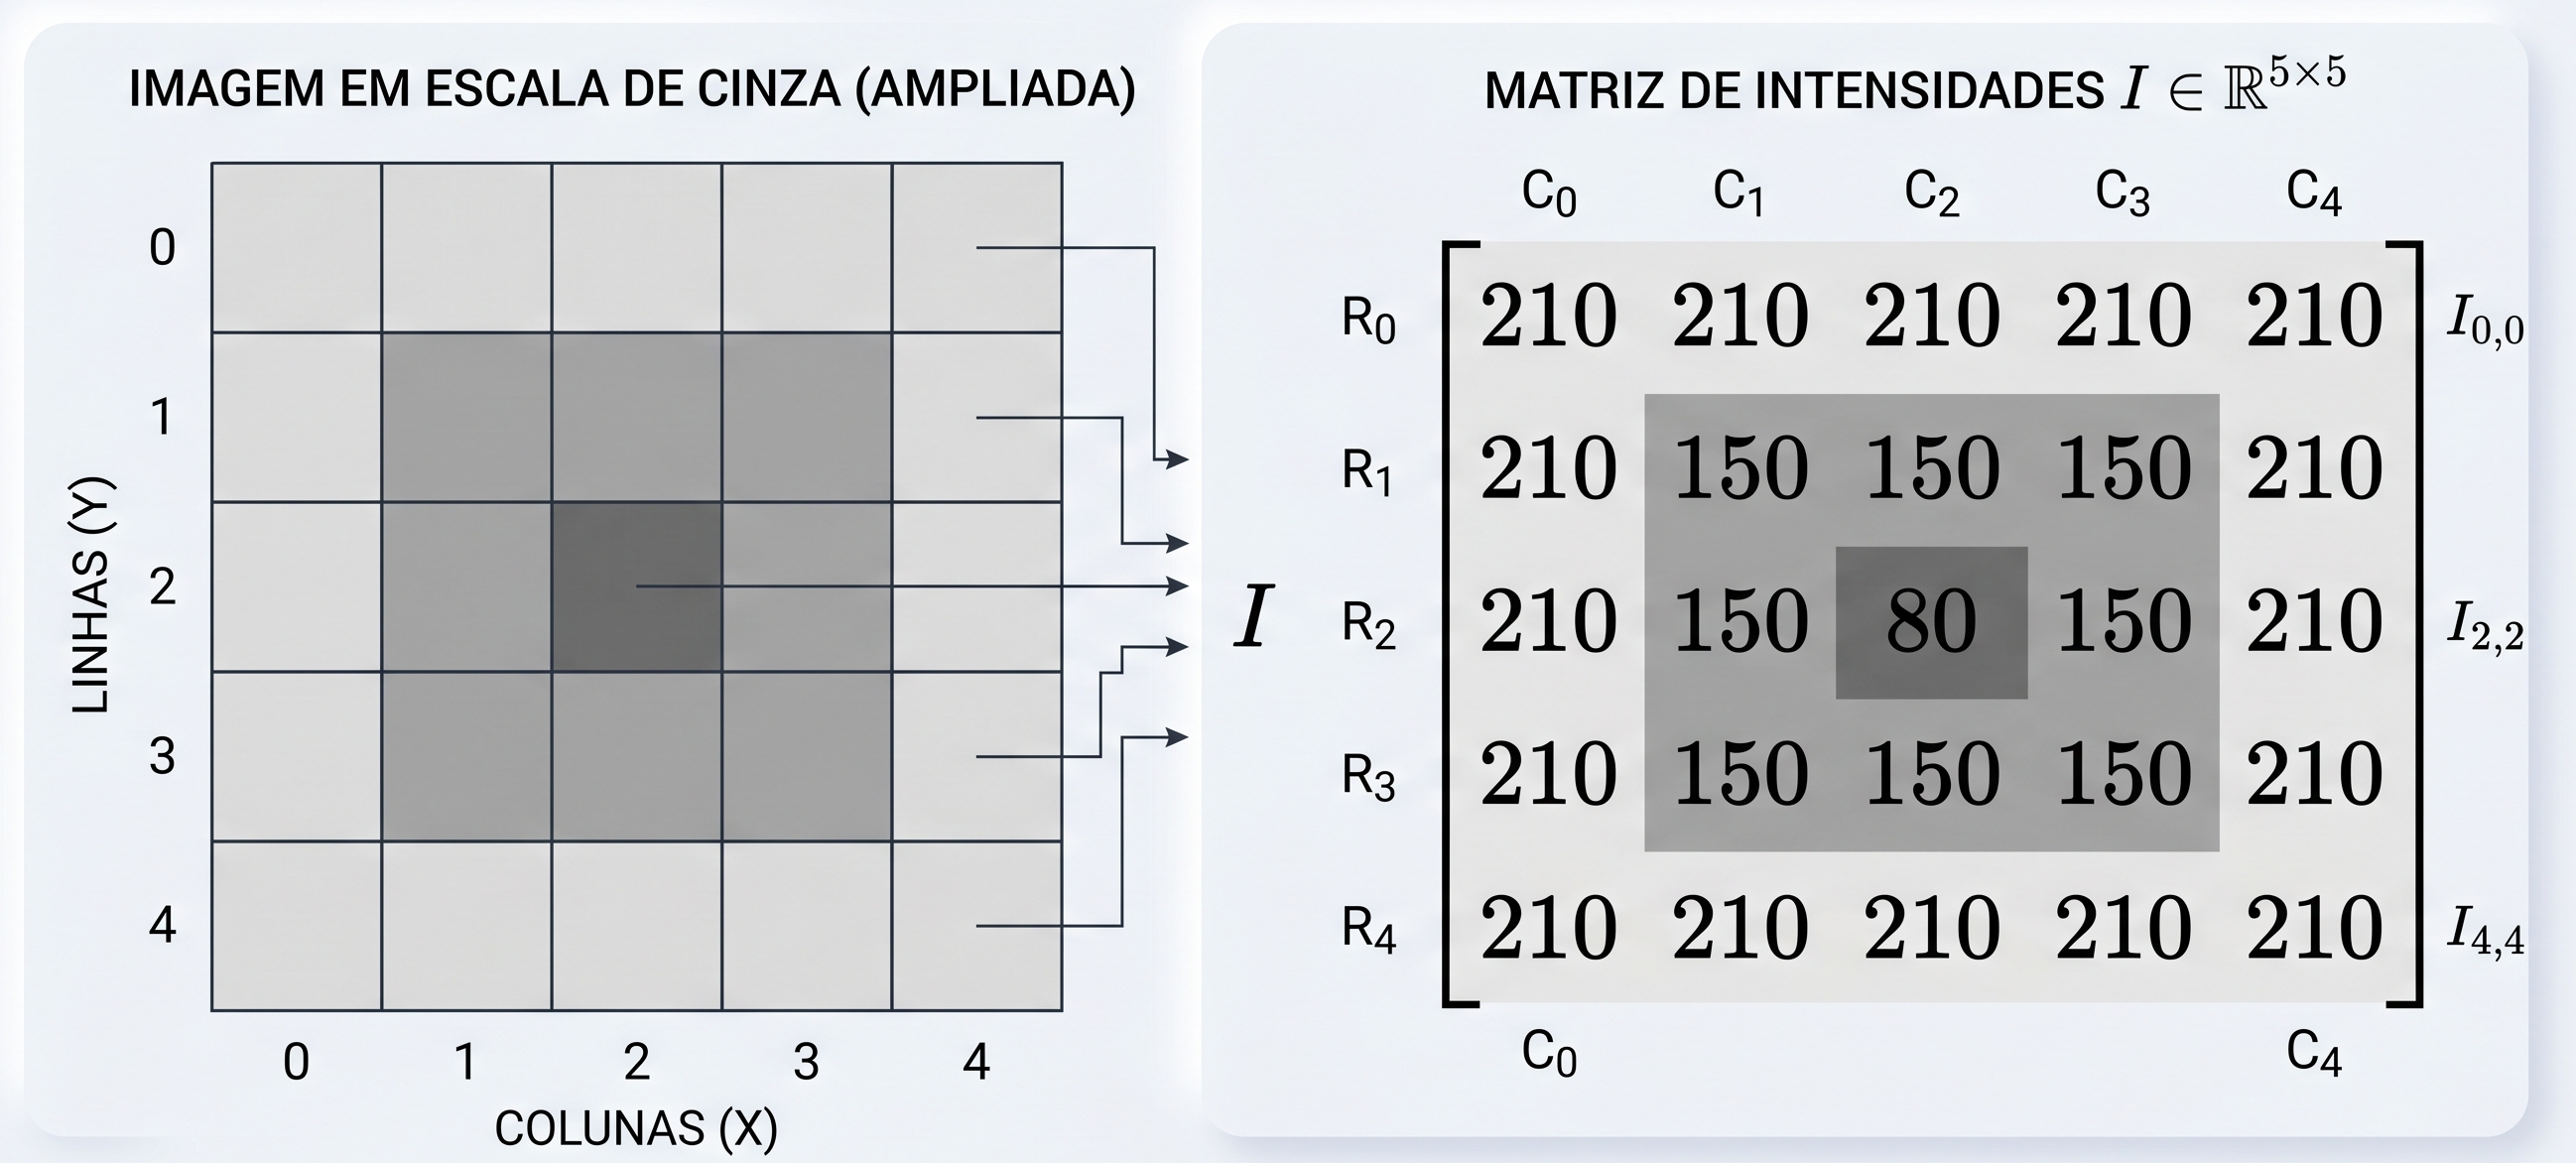
\includegraphics[width=0.72\textwidth,height=0.46\textheight,keepaspectratio]{imagem_matriz_5x5.png}
  \vspace{0.2cm}
  \begin{itemize}\small
    \item Escala de cinza: matriz 2D de intensidades; imagem RGB: tensor com 3 canais de cor
    \item As 9 bases variam de $28\times 28$ a $48\times 48$ pixels (variável no GTSRB), com 1 ou 3 canais
  \end{itemize}
  \fonte{Elaborado pelo autor (2026).}
\end{frame}

% 8 - MÉTRICAS
\begin{frame}{Métricas: por que o Macro-F1?}
  \begin{columns}[T,onlytextwidth]
    \begin{column}{0.60\textwidth}
      \centering
      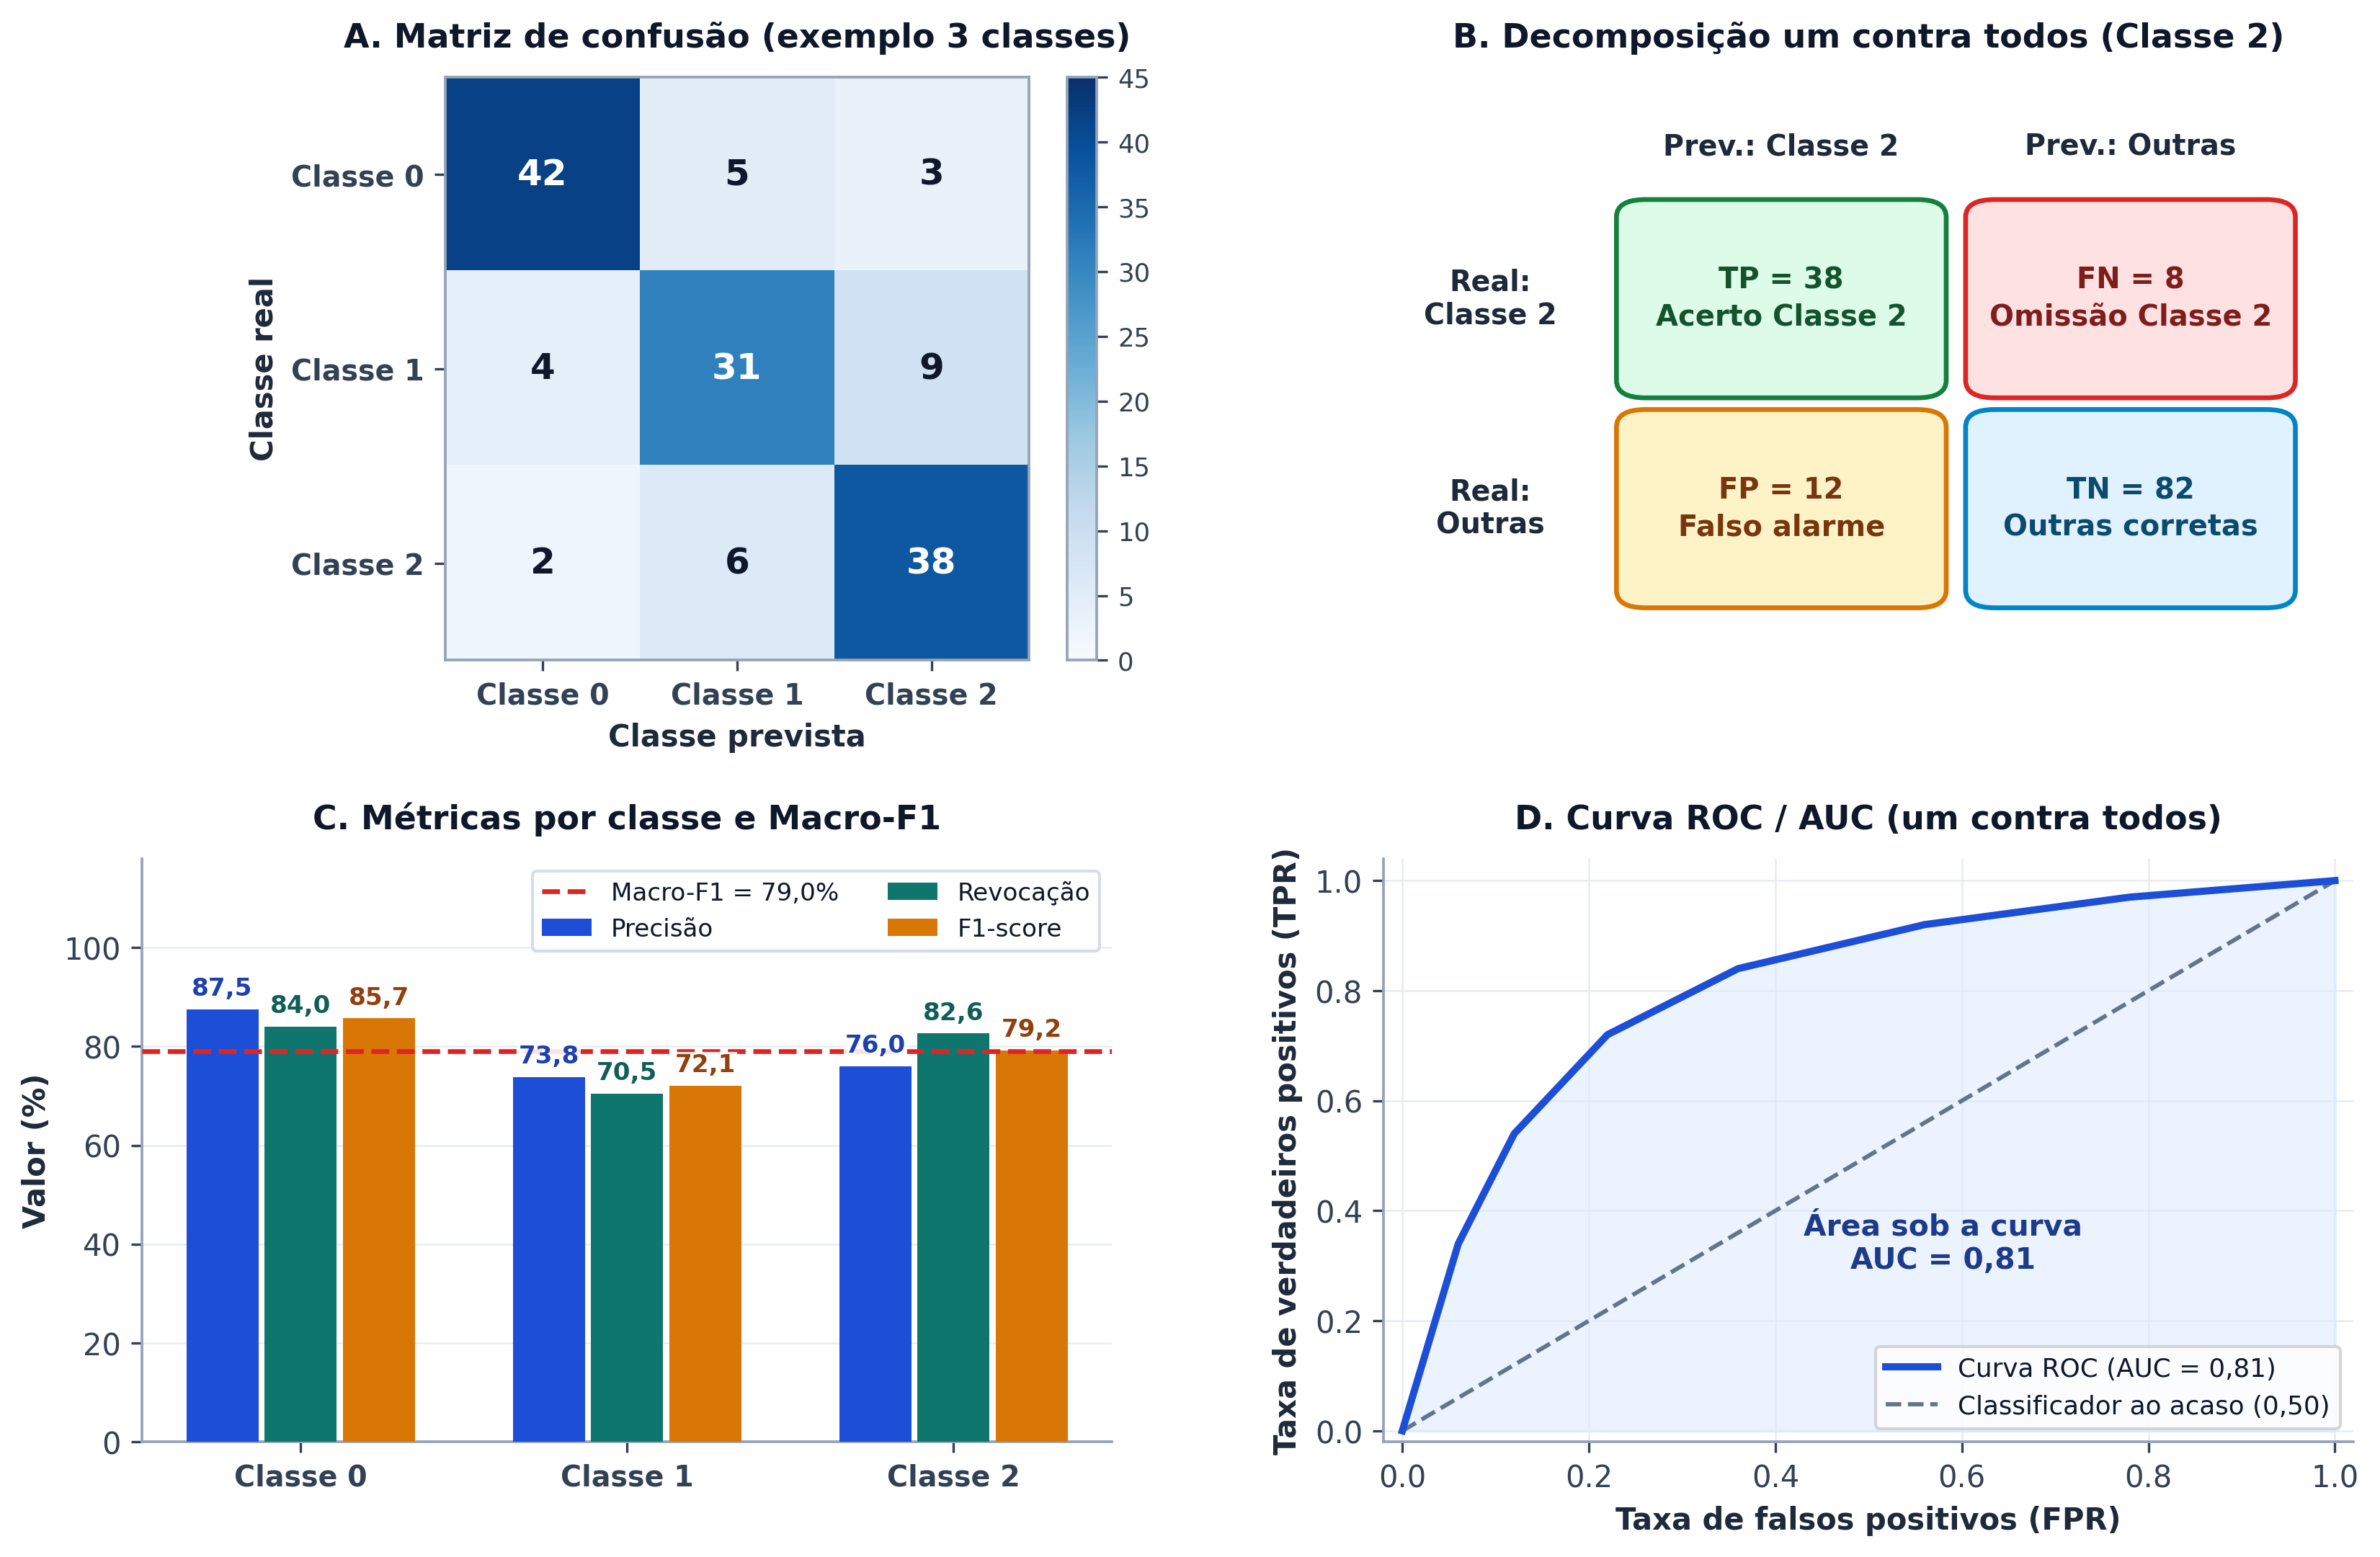
\includegraphics[width=\textwidth,height=0.70\textheight,keepaspectratio]{metricas_classificacao_exemplos.png}
    \end{column}
    \begin{column}{0.38\textwidth}
      \begin{block}{Avaliação multiclasse}
        \begin{itemize}\setlength{\itemsep}{6pt}
          \item Matriz de confusão, decomposição um-contra-todos (TP, FP, FN, TN) e curvas ROC/AUC
          \item \textbf{Macro-F1:} média não ponderada do F1 entre classes --- dá peso igual às minoritárias (SVHN, GTSRB, FER2013)
        \end{itemize}
      \end{block}
    \end{column}
  \end{columns}
  \fonte{Elaborado pelo autor (2026).}
\end{frame}

% 9 - CONVOLUÇÃO E POOLING
\begin{frame}{CNN: convolução e \textit{pooling}}
  \begin{columns}[T,onlytextwidth]
    \begin{column}{0.60\textwidth}
      \centering
      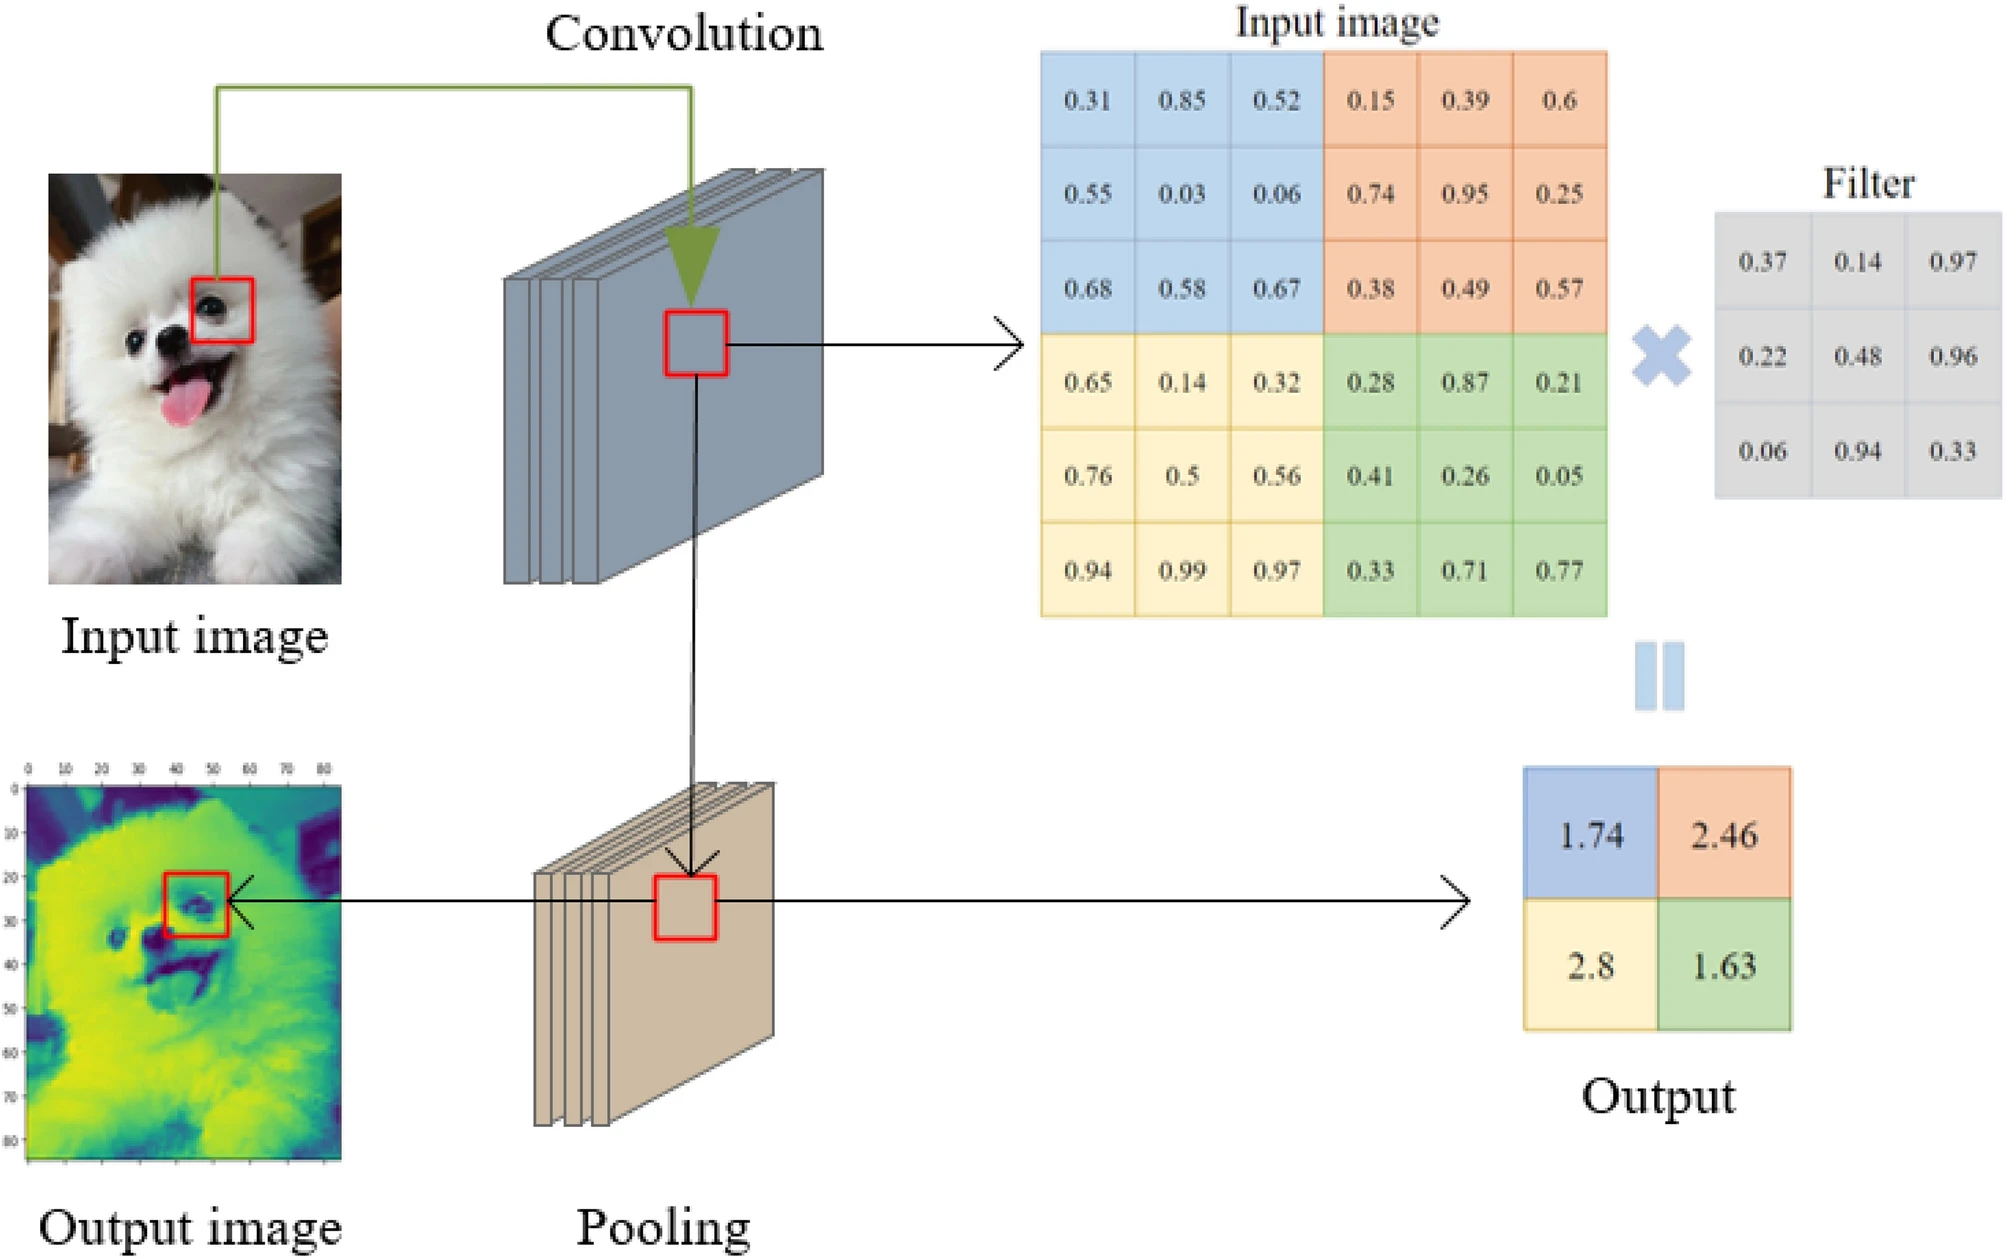
\includegraphics[width=\textwidth,height=0.70\textheight,keepaspectratio]{convolutional-pooling.png}
    \end{column}
    \begin{column}{0.38\textwidth}
      \begin{block}{Extração hierárquica}
        \begin{itemize}\setlength{\itemsep}{6pt}
          \item Filtros treináveis percorrem a imagem e detectam padrões espaciais locais
          \item \textit{Pooling} reduz a resolução espacial progressivamente e preserva atributos discriminativos
        \end{itemize}
      \end{block}
    \end{column}
  \end{columns}
  \fonte{adaptado de Zhao e Zhang (2024).}
\end{frame}

% 9b - SEPARABLECONV2D ETAPA 1 (DEPTHWISE)
\begin{frame}{Convolução separável: Etapa 1 --- \textit{Depthwise} $3\times 3$}
  \centering
  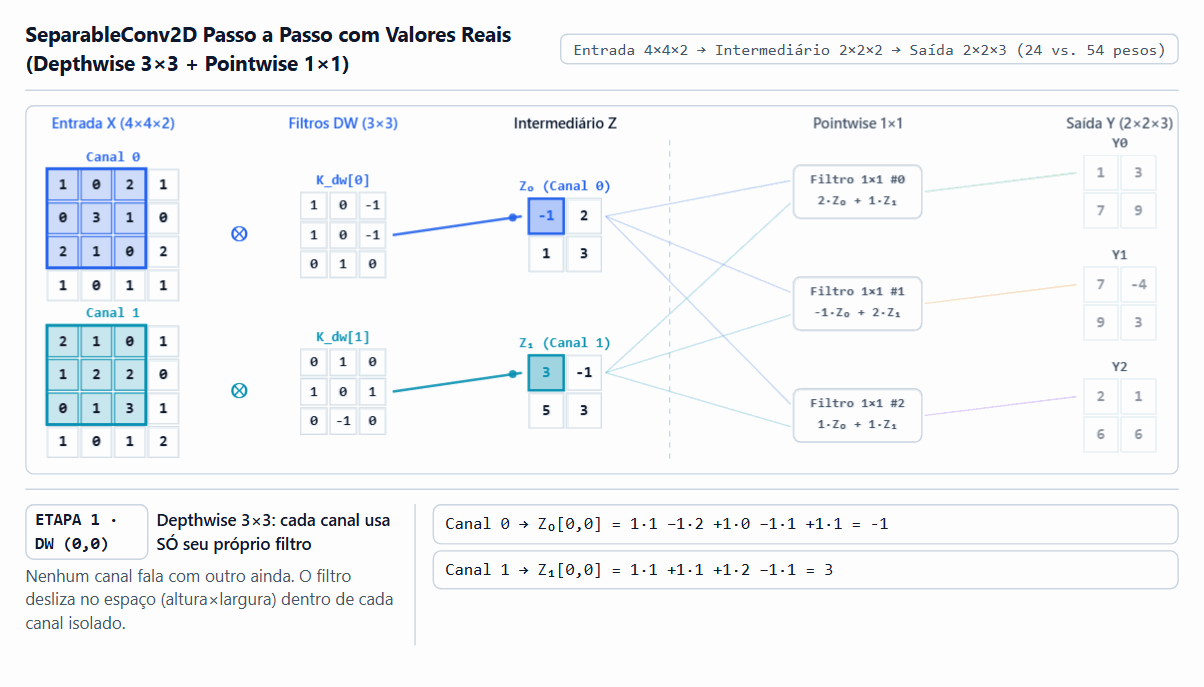
\includegraphics[width=0.98\textwidth,height=0.56\textheight,keepaspectratio]{fig_sepconv2d_etapa1_depthwise.png}
  \vspace{0.10cm}
  \begin{itemize}\footnotesize
    \item Cada canal de entrada ($4\times 4\times 2$) aplica isoladamente seu próprio filtro espacial $3\times 3$ (18 pesos na etapa DW)
    \item Produz o tensor intermediário $Z$ ($2\times 2\times 2$) antes de qualquer combinação entre canais
  \end{itemize}
  \fonte{Elaborado pelo autor (2026).}
\end{frame}

% 9c - SEPARABLECONV2D ETAPA 2 (POINTWISE)
\begin{frame}{Convolução separável: Etapa 2 --- \textit{Pointwise} $1\times 1$}
  \centering
  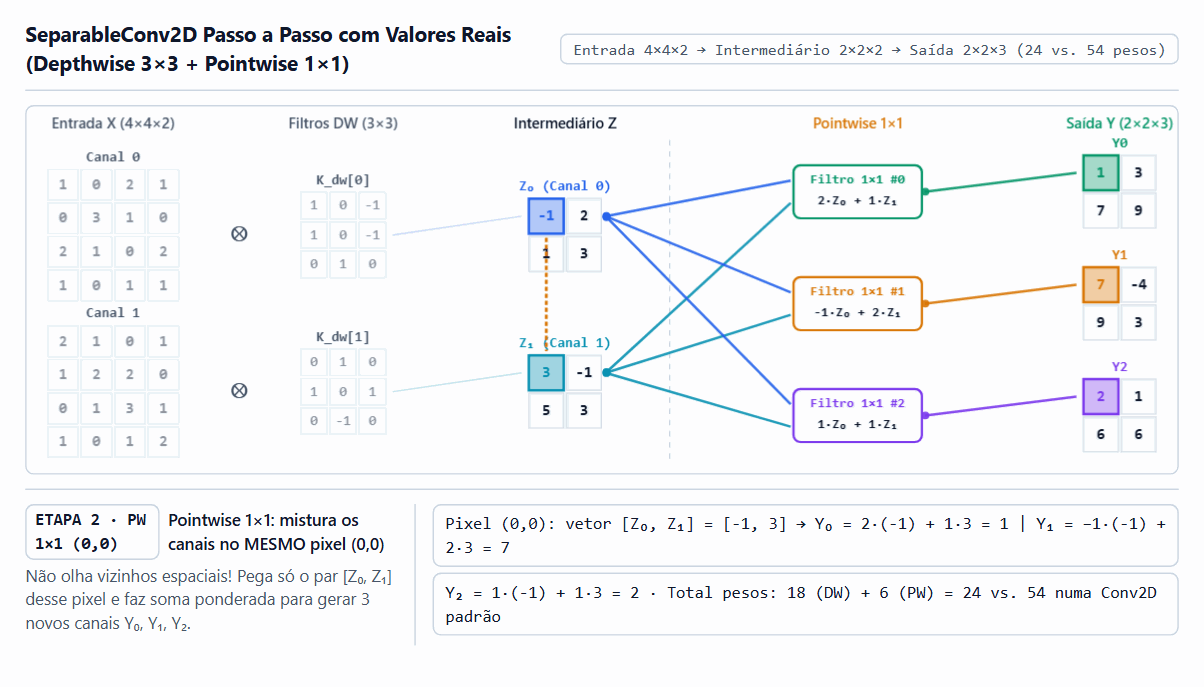
\includegraphics[width=0.98\textwidth,height=0.56\textheight,keepaspectratio]{fig_sepconv2d_etapa2_pointwise.png}
  \vspace{0.10cm}
  \begin{itemize}\footnotesize
    \item Três filtros $1\times 1$ combinam linearmente o par $[Z_0, Z_1]$ em cada posição espacial (6 pesos na etapa PW)
    \item Gera a saída $2\times 2\times 3$ usando \textbf{24 pesos totais} frente a 54 pesos em uma \texttt{Conv2D} padrão equivalente
  \end{itemize}
  \fonte{Elaborado pelo autor (2026).}
\end{frame}

% 10 - MAPAS DE CARACTERÍSTICAS
\begin{frame}{Mapas de características em entradas $64\times 64\times 1$}
  \begin{columns}[T,onlytextwidth]
    \begin{column}{0.315\textwidth}
      \centering
      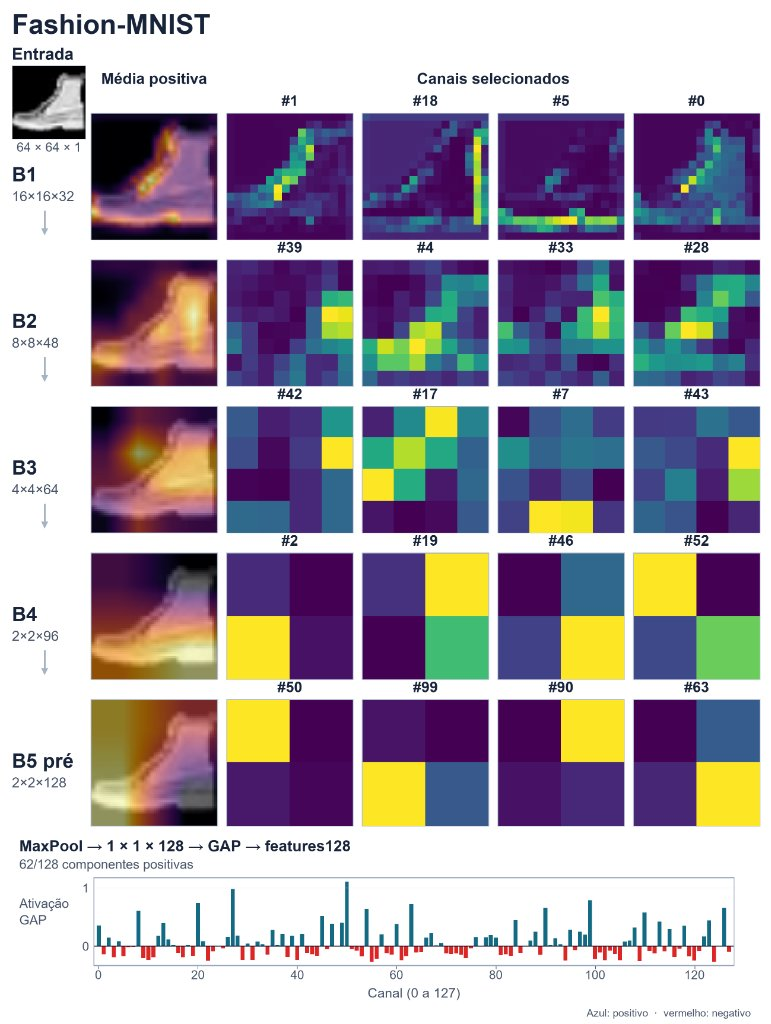
\includegraphics[width=\textwidth,height=0.72\textheight,keepaspectratio]{fmap_03a_piramide_blocos_fashion_mnist.png}
    \end{column}
    \begin{column}{0.315\textwidth}
      \centering
      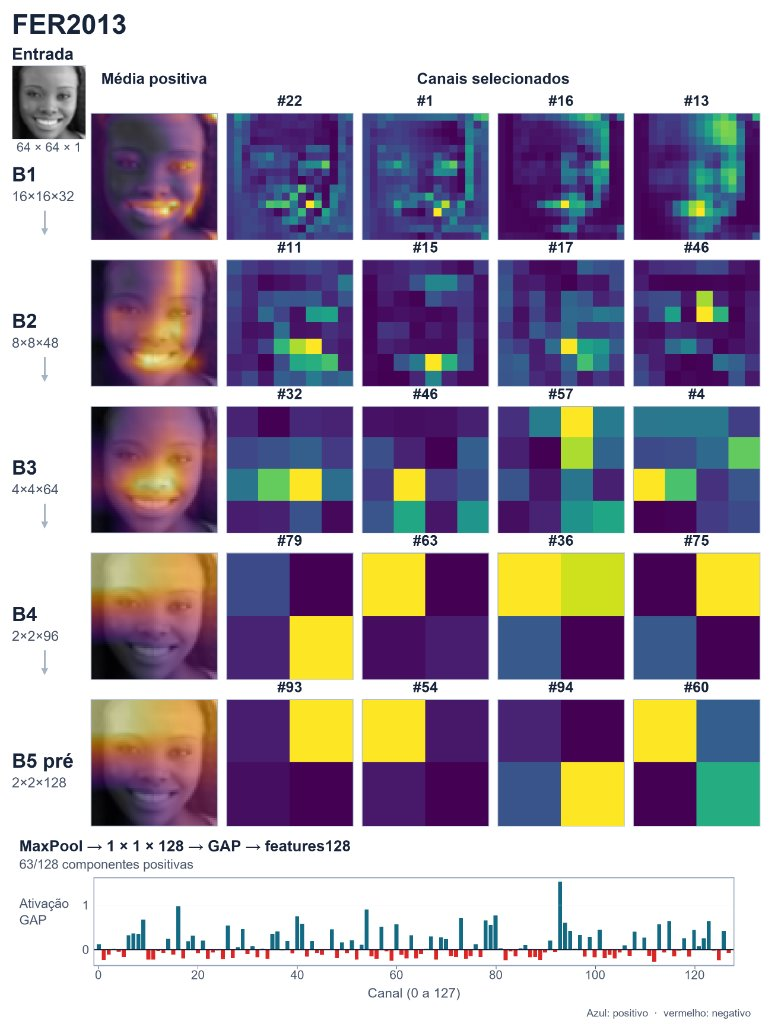
\includegraphics[width=\textwidth,height=0.72\textheight,keepaspectratio]{fmap_03b_piramide_blocos_fer2013.png}
    \end{column}
    \begin{column}{0.34\textwidth}
      \begin{block}{Hierarquia de ativações}
        \begin{itemize}\setlength{\itemsep}{4pt}
          \item \textbf{B1--B2:} bordas e contornos locais (bota; olhos e sorriso)
          \item \textbf{B3--B5:} foco crescente na região semântica do objeto
          \item \textbf{GAP $\to$ \texttt{features128}:} 62/128 positivos (Fashion) e 63/128 (FER2013)
          \item Mínimo negativo em $-0{,}2785$ (curva SiLU)
        \end{itemize}
      \end{block}
    \end{column}
  \end{columns}
  \fonte{Elaborado pelo autor (2026).}
\end{frame}

% 11 - AUMENTO DE DADOS: PIPELINE COMPOSTO
\begin{frame}{Aumento de dados: pipeline composto em 6 etapas}
  \centering
  {\footnotesize\bfseries\color{senacblue}(a) GTSRB ($128\times 128\times 3$ --- placa PARE) \;|\; RMS = 0,2967}\\[-1pt]
  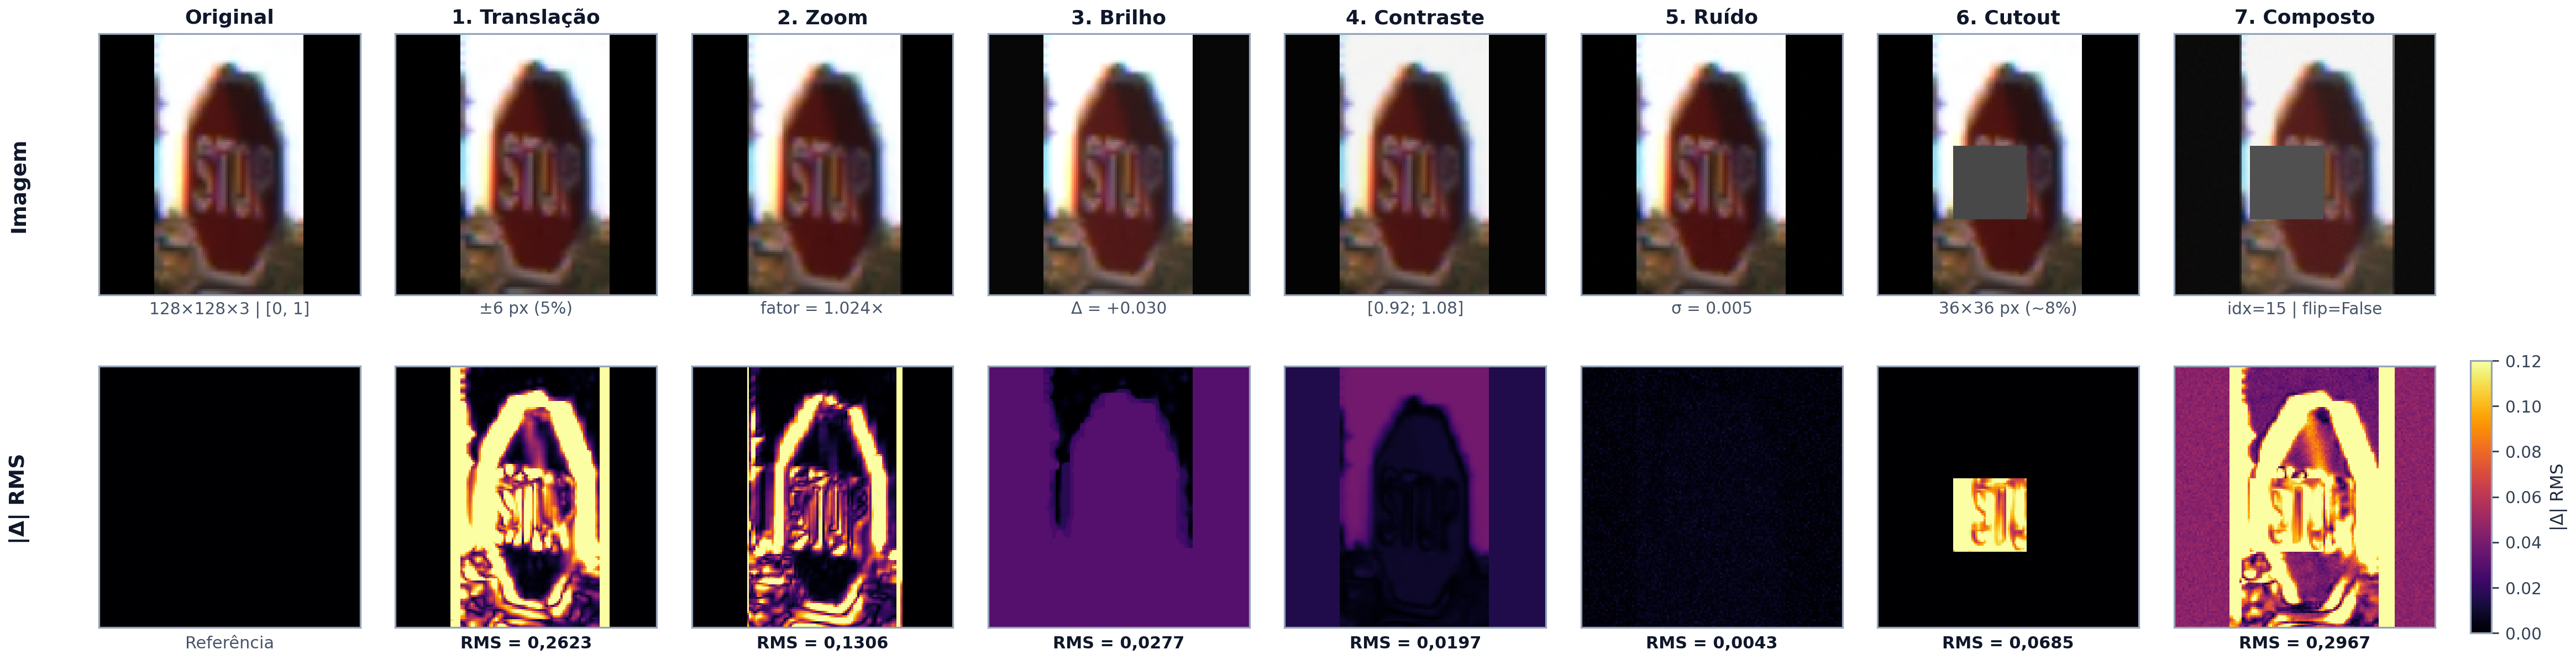
\includegraphics[width=0.95\textwidth,height=0.23\textheight,keepaspectratio]{aug_01_pipeline_etapas_gtsrb.png}
  \vspace{0.04cm}

  {\footnotesize\bfseries\color{senacblue}(b) CIFAR-10 ($64\times 64\times 3$ --- navio) \;|\; RMS = 0,1084}\\[-1pt]
  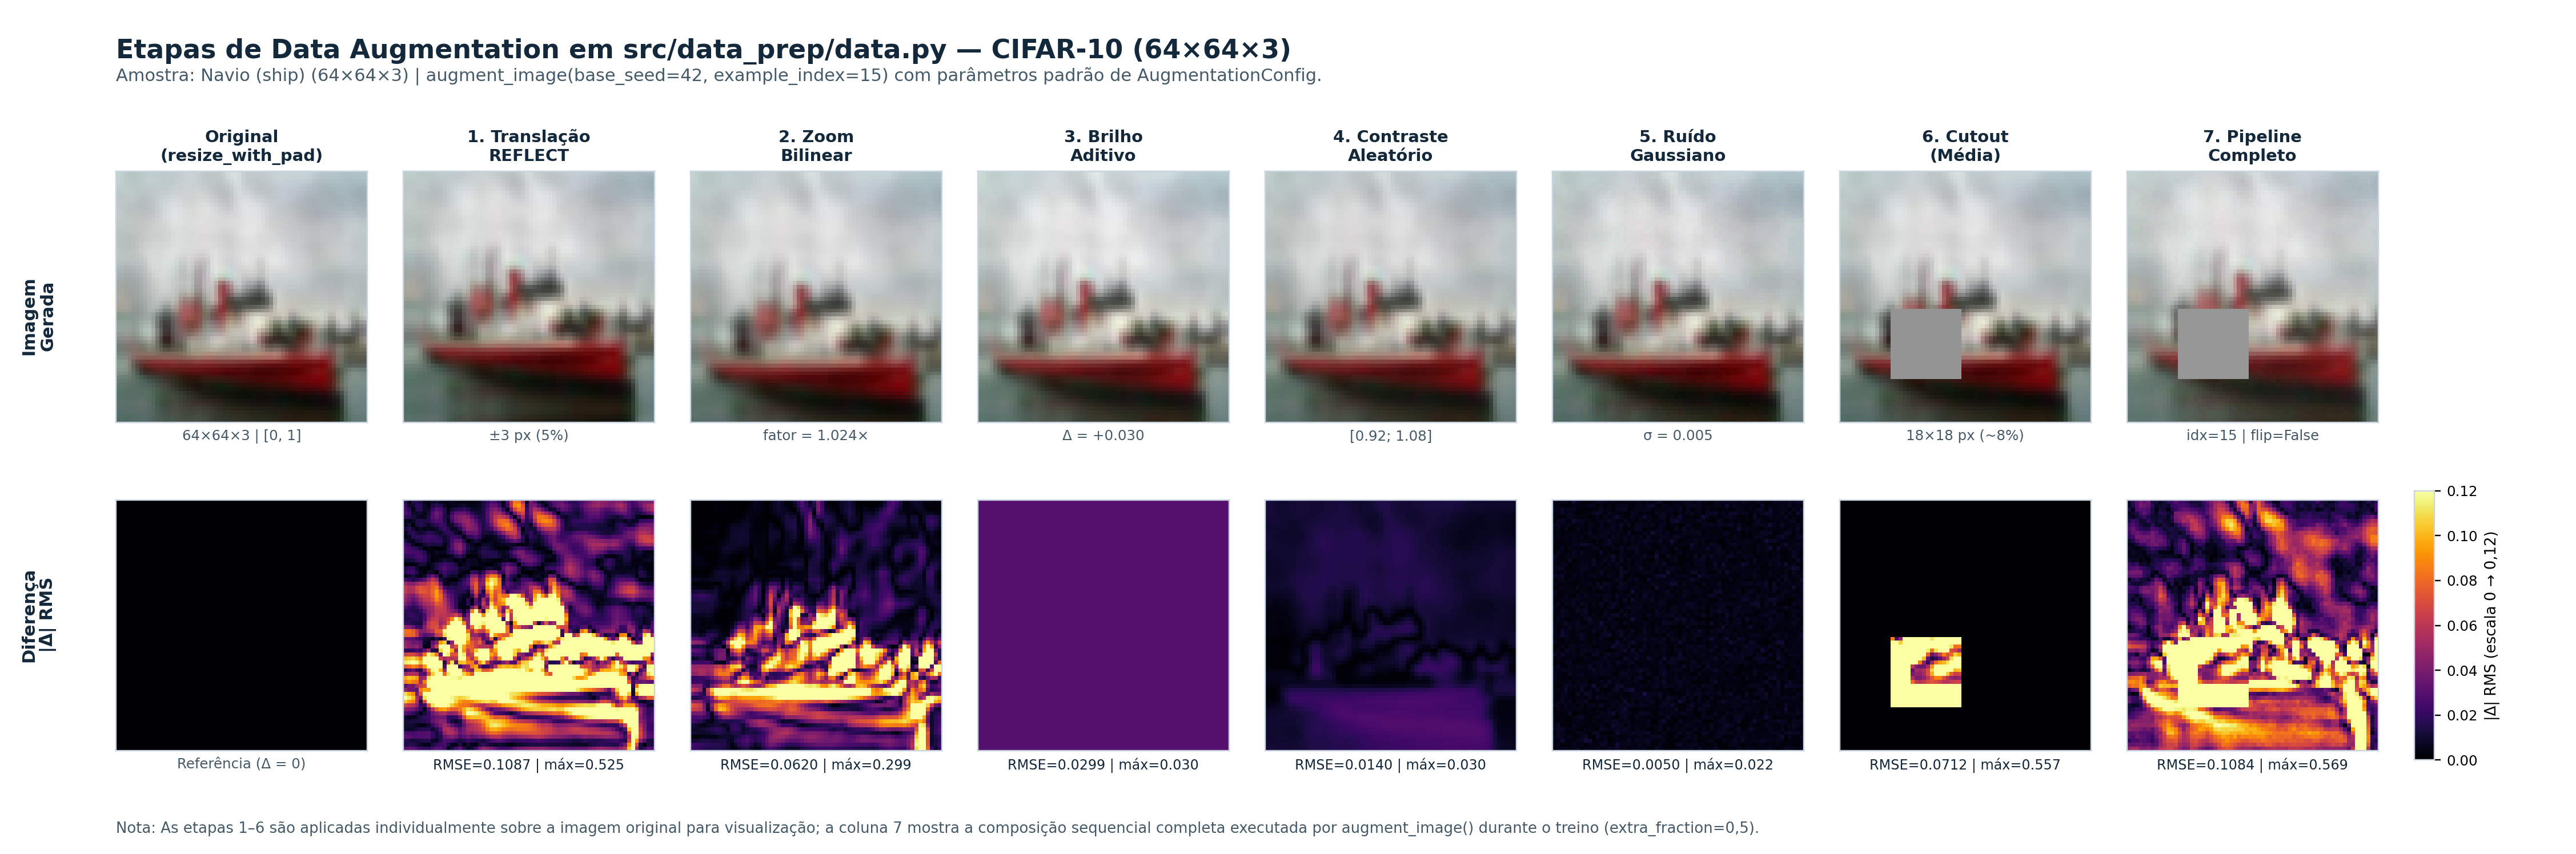
\includegraphics[width=0.95\textwidth,height=0.23\textheight,keepaspectratio]{aug_02_pipeline_etapas_cifar10.png}
  \vspace{0.04cm}

  {\footnotesize Etapas: translação $\pm 5\%$, zoom $[0{,}96;1{,}04]$, brilho $\pm 0{,}03$, contraste $[0{,}92;1{,}08]$, ruído $\sigma=0{,}005$ e \textit{cutout} $\sim 8\%$.}
  \fonte{Elaborado pelo autor (2026).}
\end{frame}

% 12 - PRESERVAÇÃO SEMÂNTICA E flip_lr=False
\begin{frame}{Preservação semântica e \texttt{flip\_lr=False}}
  \begin{columns}[T,onlytextwidth]
    \begin{column}{0.60\textwidth}
      \centering
      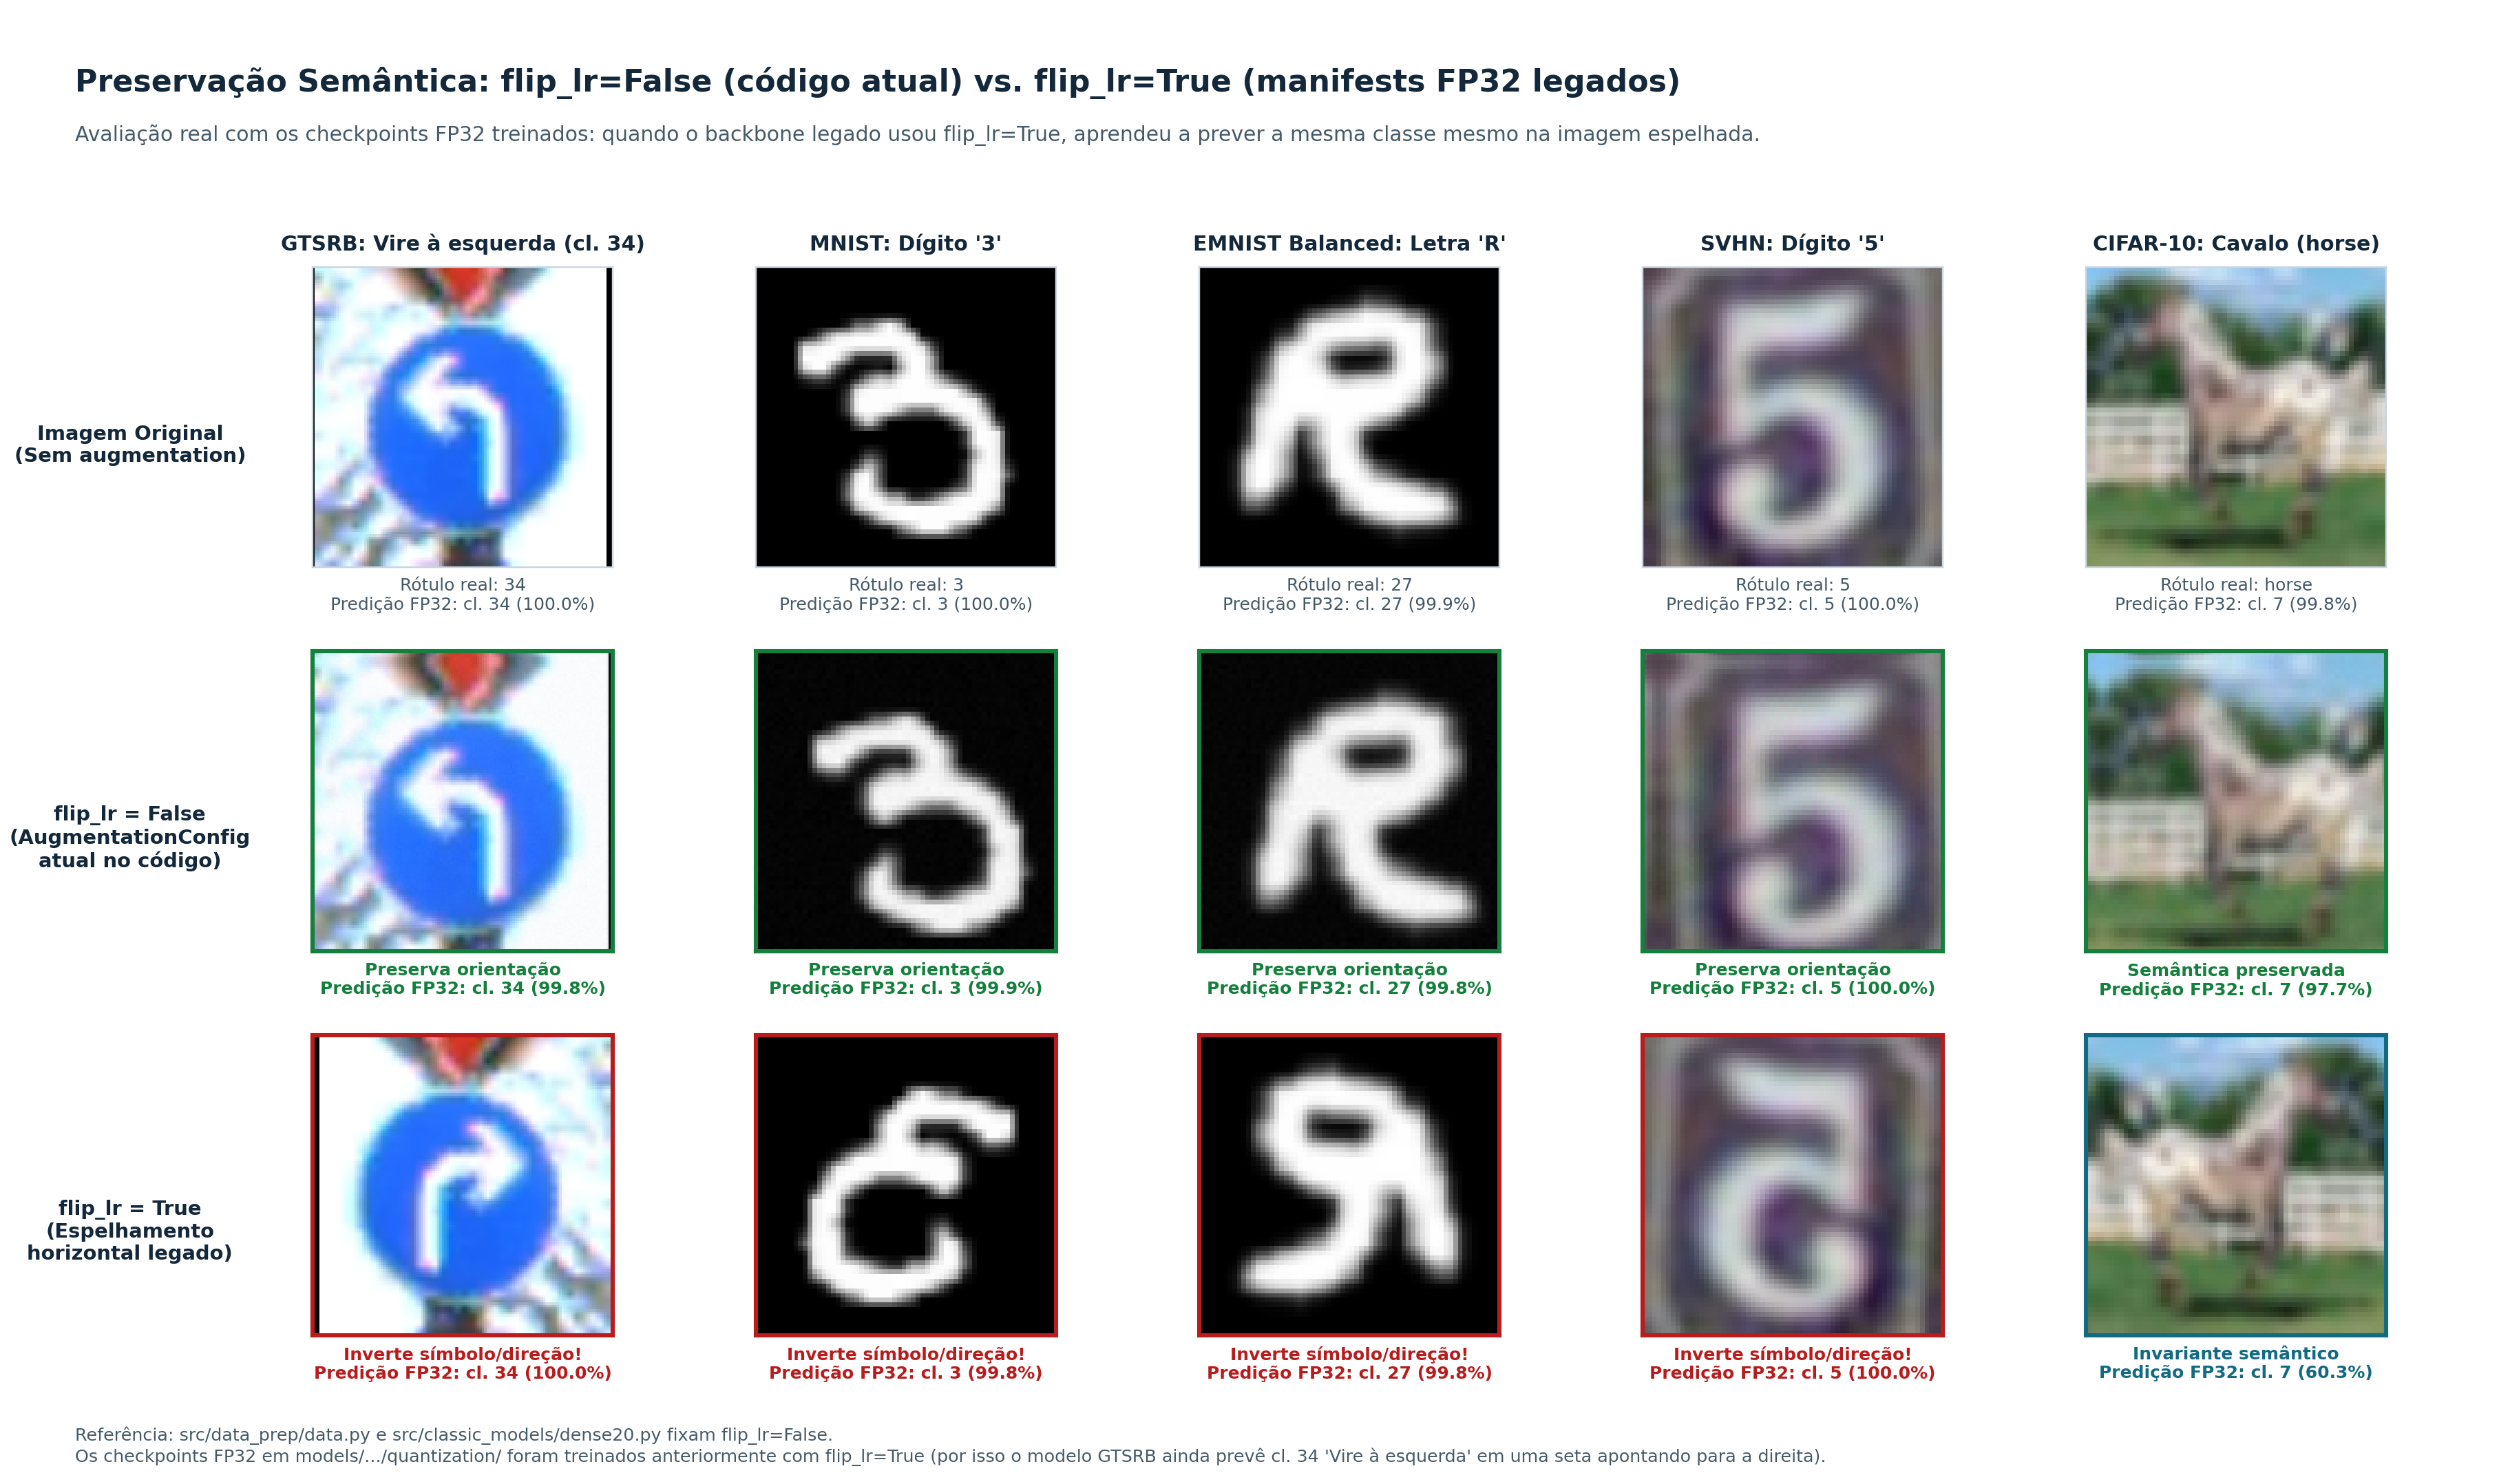
\includegraphics[width=\textwidth,height=0.68\textheight,keepaspectratio]{aug_03_comparacao_flip_lr_semantico.png}
    \end{column}
    \begin{column}{0.38\textwidth}
      \begin{block}{Por que remover o \textit{flip}?}
        \begin{itemize}\setlength{\itemsep}{5pt}
          \item \textcolor{badred}{\textbf{Inversão de classe:}} espelhar altera GTSRB (``vire à esquerda''), MNIST (``3''), EMNIST (``R'') e SVHN (``5'')
          \item \textcolor{okgreen}{\textbf{Invariância restrita:}} válido só em objetos naturais (ex.: cavalo no CIFAR-10)
          \item \textbf{Correção:} fixado \texttt{flip\_lr=False} em \texttt{src/data\_prep/data.py}
        \end{itemize}
      \end{block}
    \end{column}
  \end{columns}
  \fonte{Elaborado pelo autor (2026).}
\end{frame}

% 13 - QUBITS, SUPERPOSIÇÃO E EMARANHAMENTO
\begin{frame}{Qubits, superposição, emaranhamento e medição}
  \begin{columns}[T,onlytextwidth]
    \begin{column}{0.48\textwidth}
      \centering
      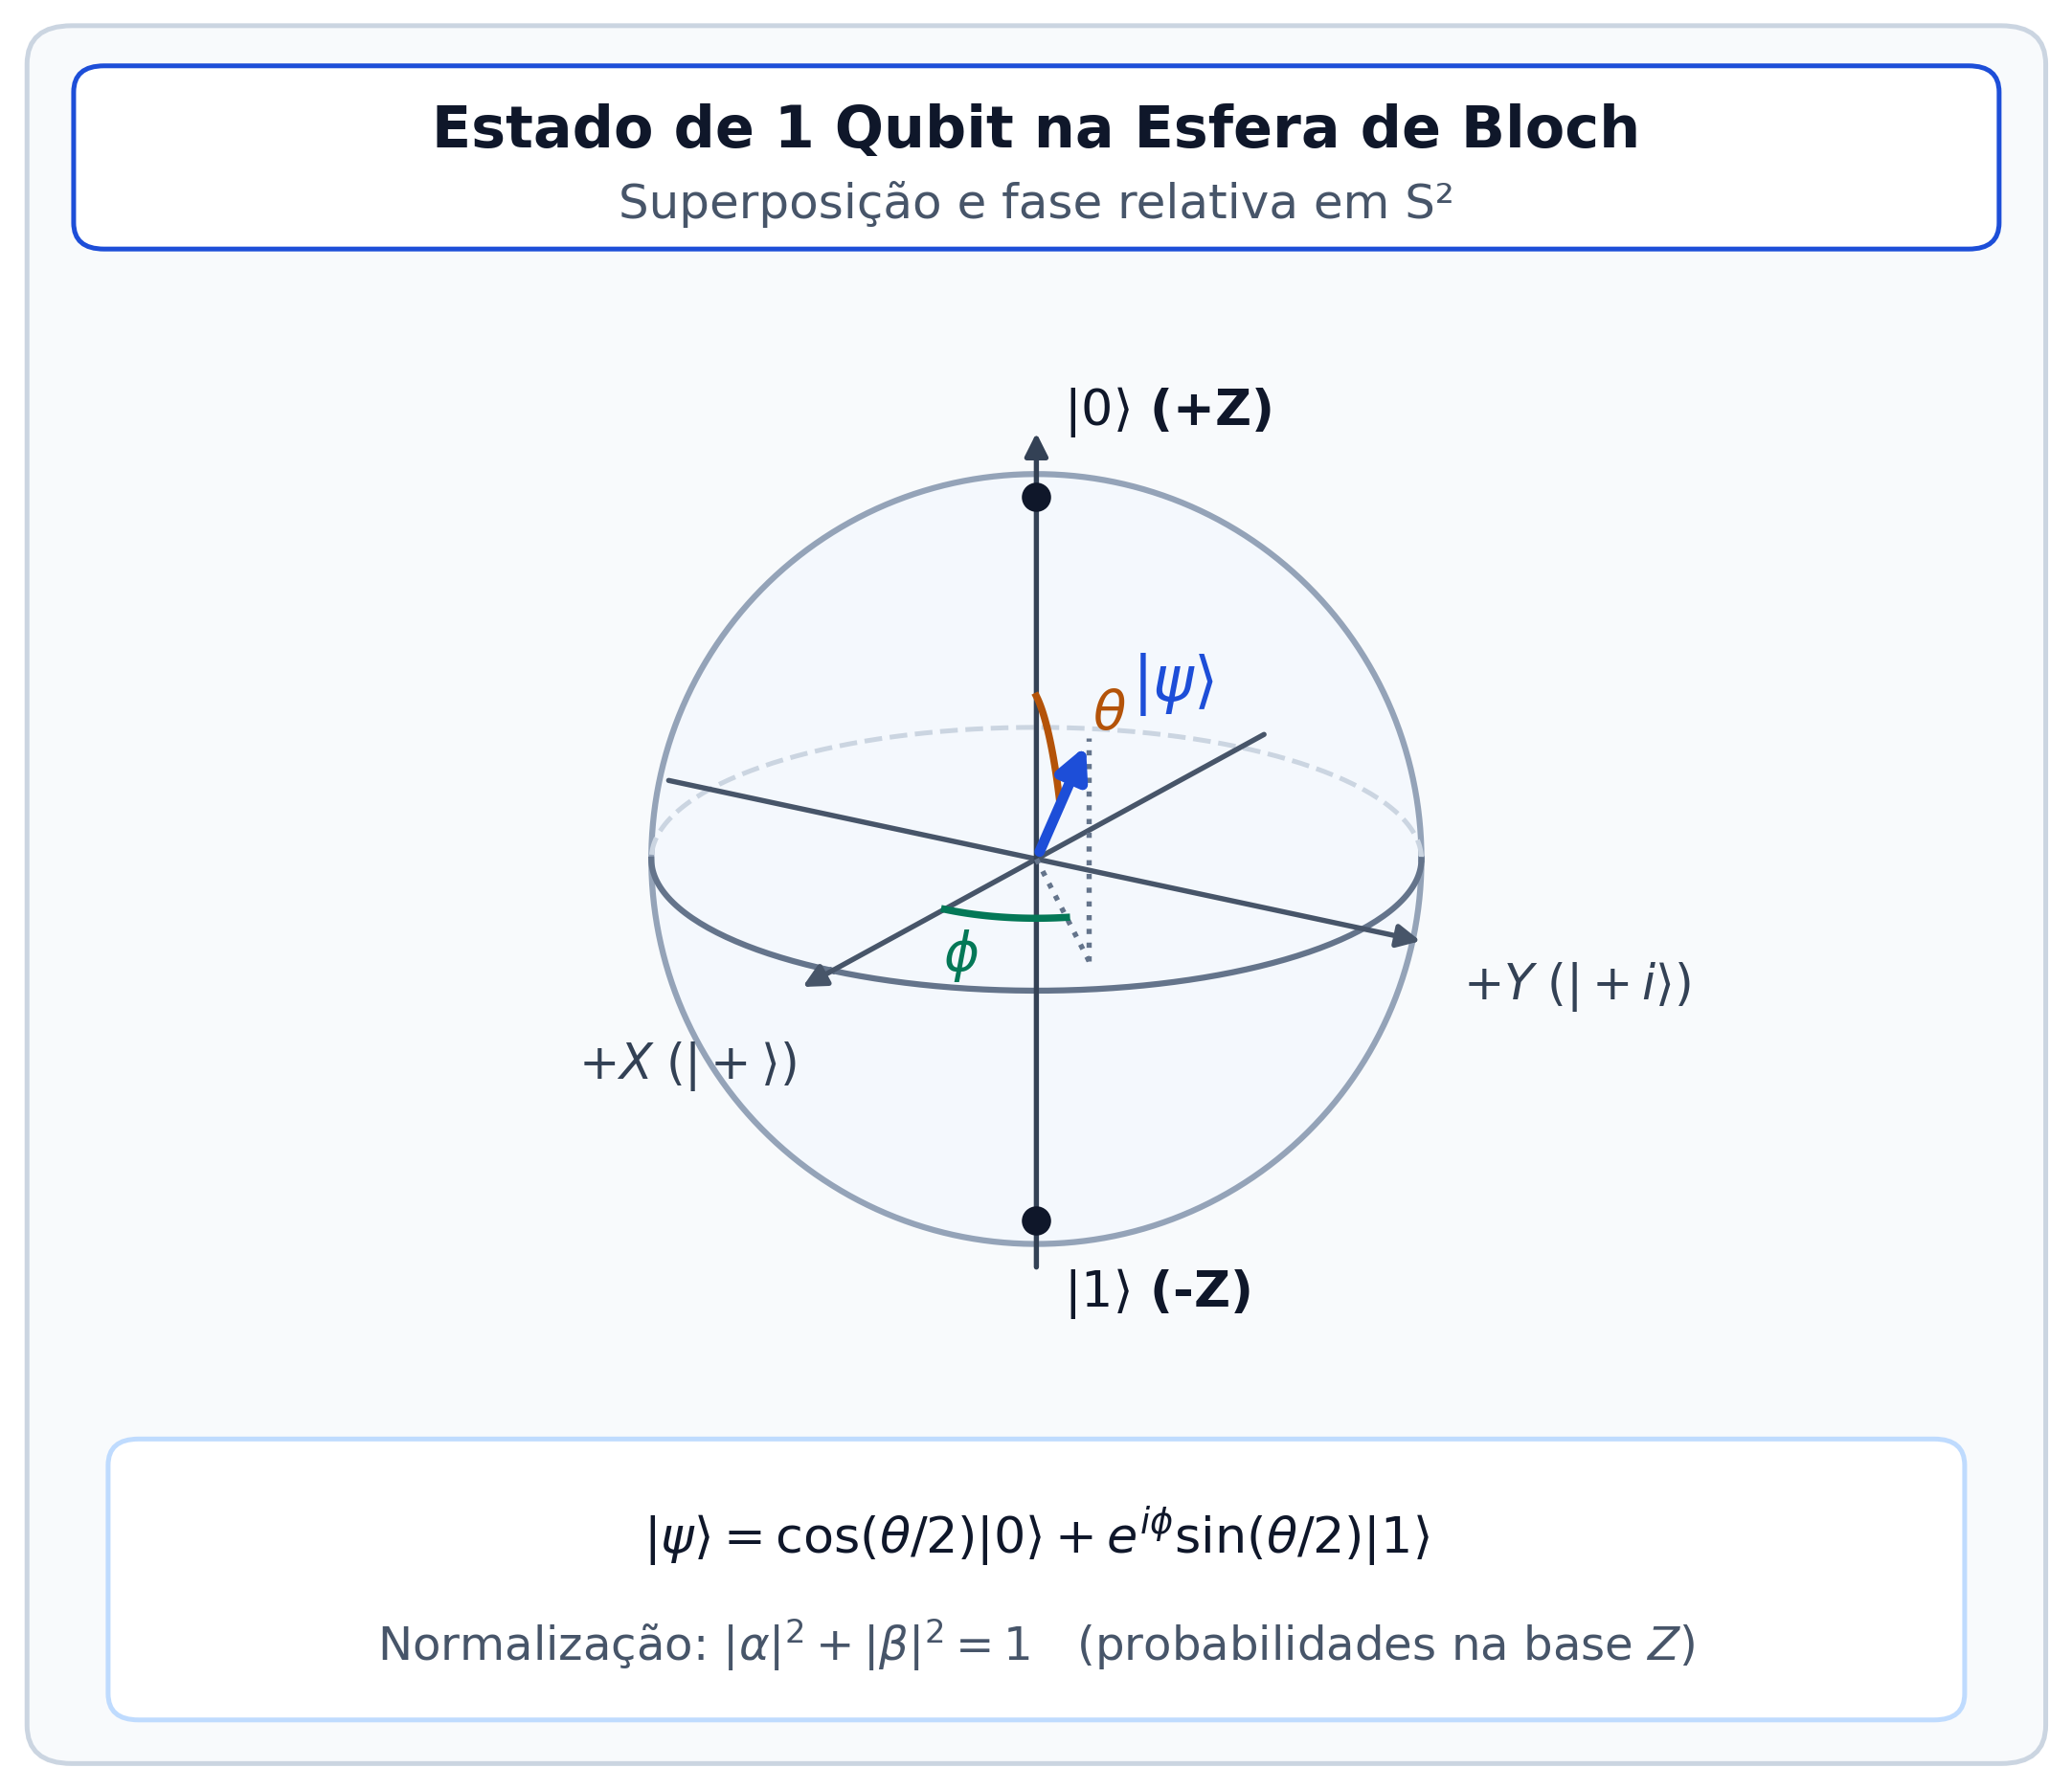
\includegraphics[width=\textwidth,height=0.48\textheight,keepaspectratio]{fig_261_esfera_bloch.png}
    \end{column}
    \begin{column}{0.48\textwidth}
      \centering
      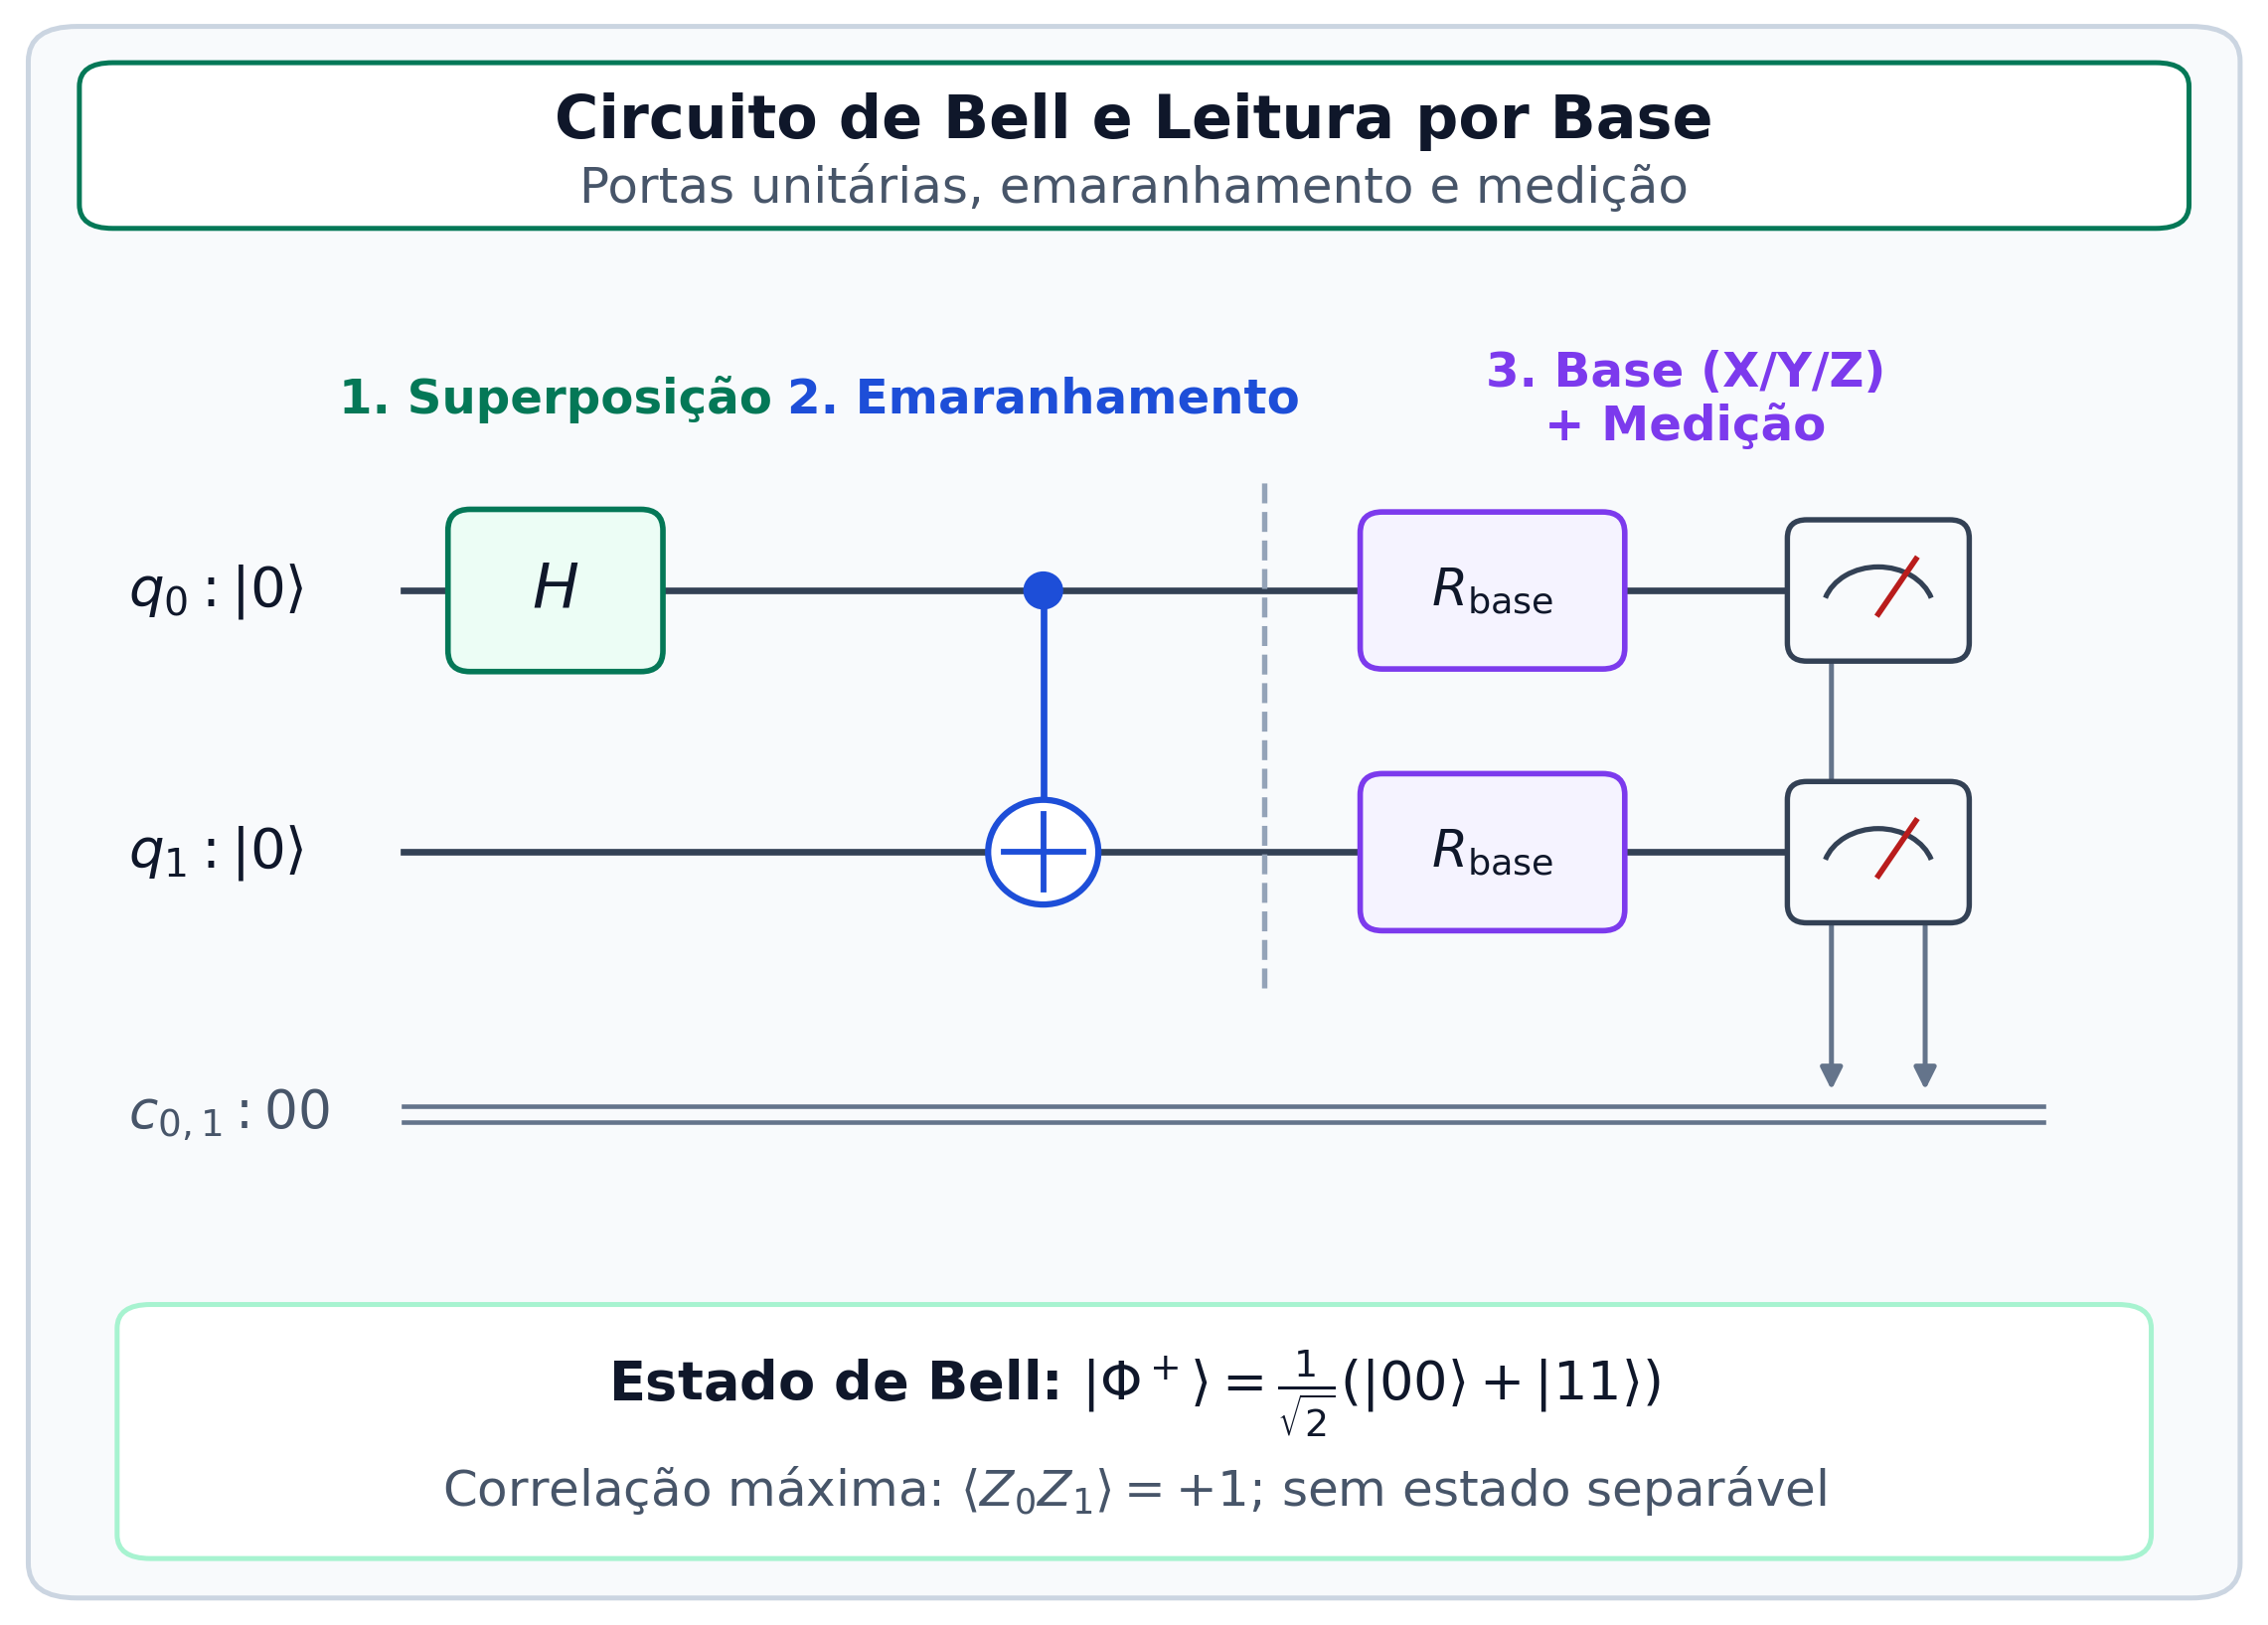
\includegraphics[width=\textwidth,height=0.48\textheight,keepaspectratio]{fig_261_circuito_bell.png}
    \end{column}
  \end{columns}
  \vspace{0.15cm}
  \begin{itemize}\footnotesize
    \item Qubit na esfera de Bloch: superposição de $\ket{0}$ e $\ket{1}$ manipulada por rotações unitárias
    \item Portas $H$ e CNOT geram emaranhamento (estado de Bell); medição extrai valores esperados reais
  \end{itemize}
  \fonte{Elaborado pelo autor (2026), com base em Nielsen e Chuang (2010) e IBM Quantum (2026).}
\end{frame}

% 14 - CODIFICAÇÃO DE DADOS E LAÇO VQA
\begin{frame}{Codificação de dados e laço variacional (VQA)}
  \begin{columns}[T,onlytextwidth]
    \begin{column}{0.48\textwidth}
      \centering
      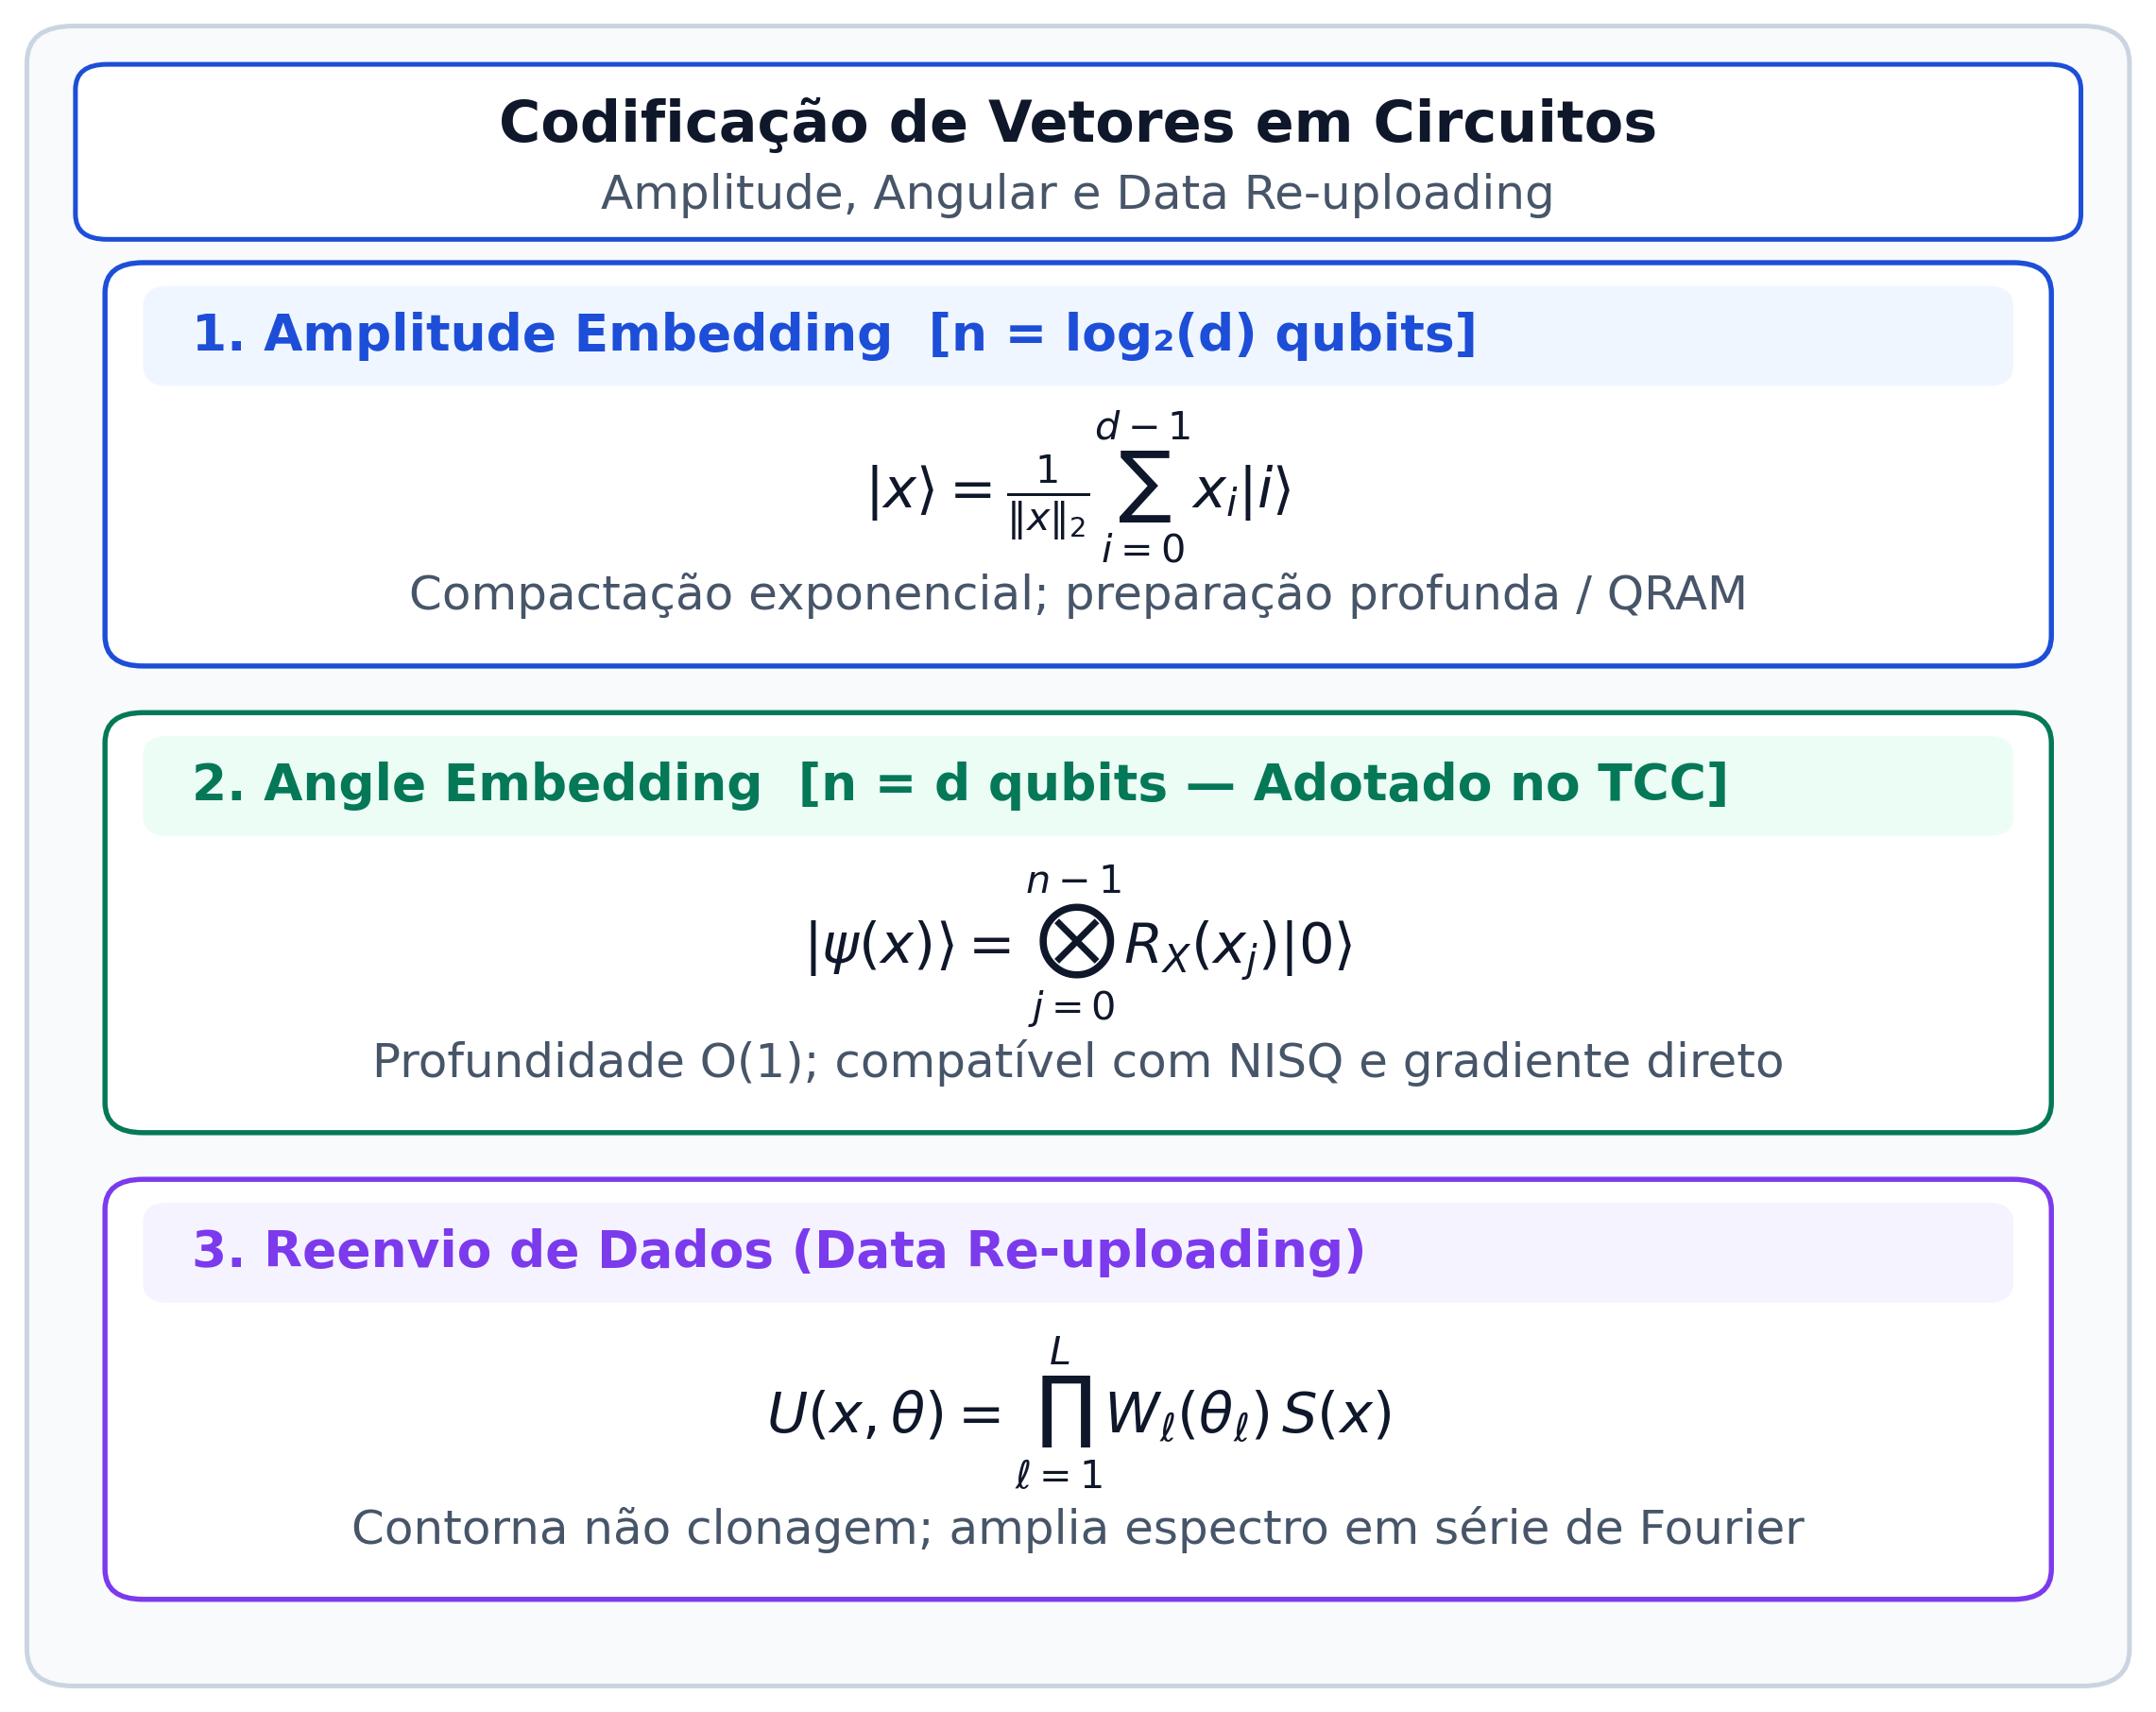
\includegraphics[width=\textwidth,height=0.46\textheight,keepaspectratio]{fig_263_codificacoes_vetoriais.png}
    \end{column}
    \begin{column}{0.48\textwidth}
      \centering
      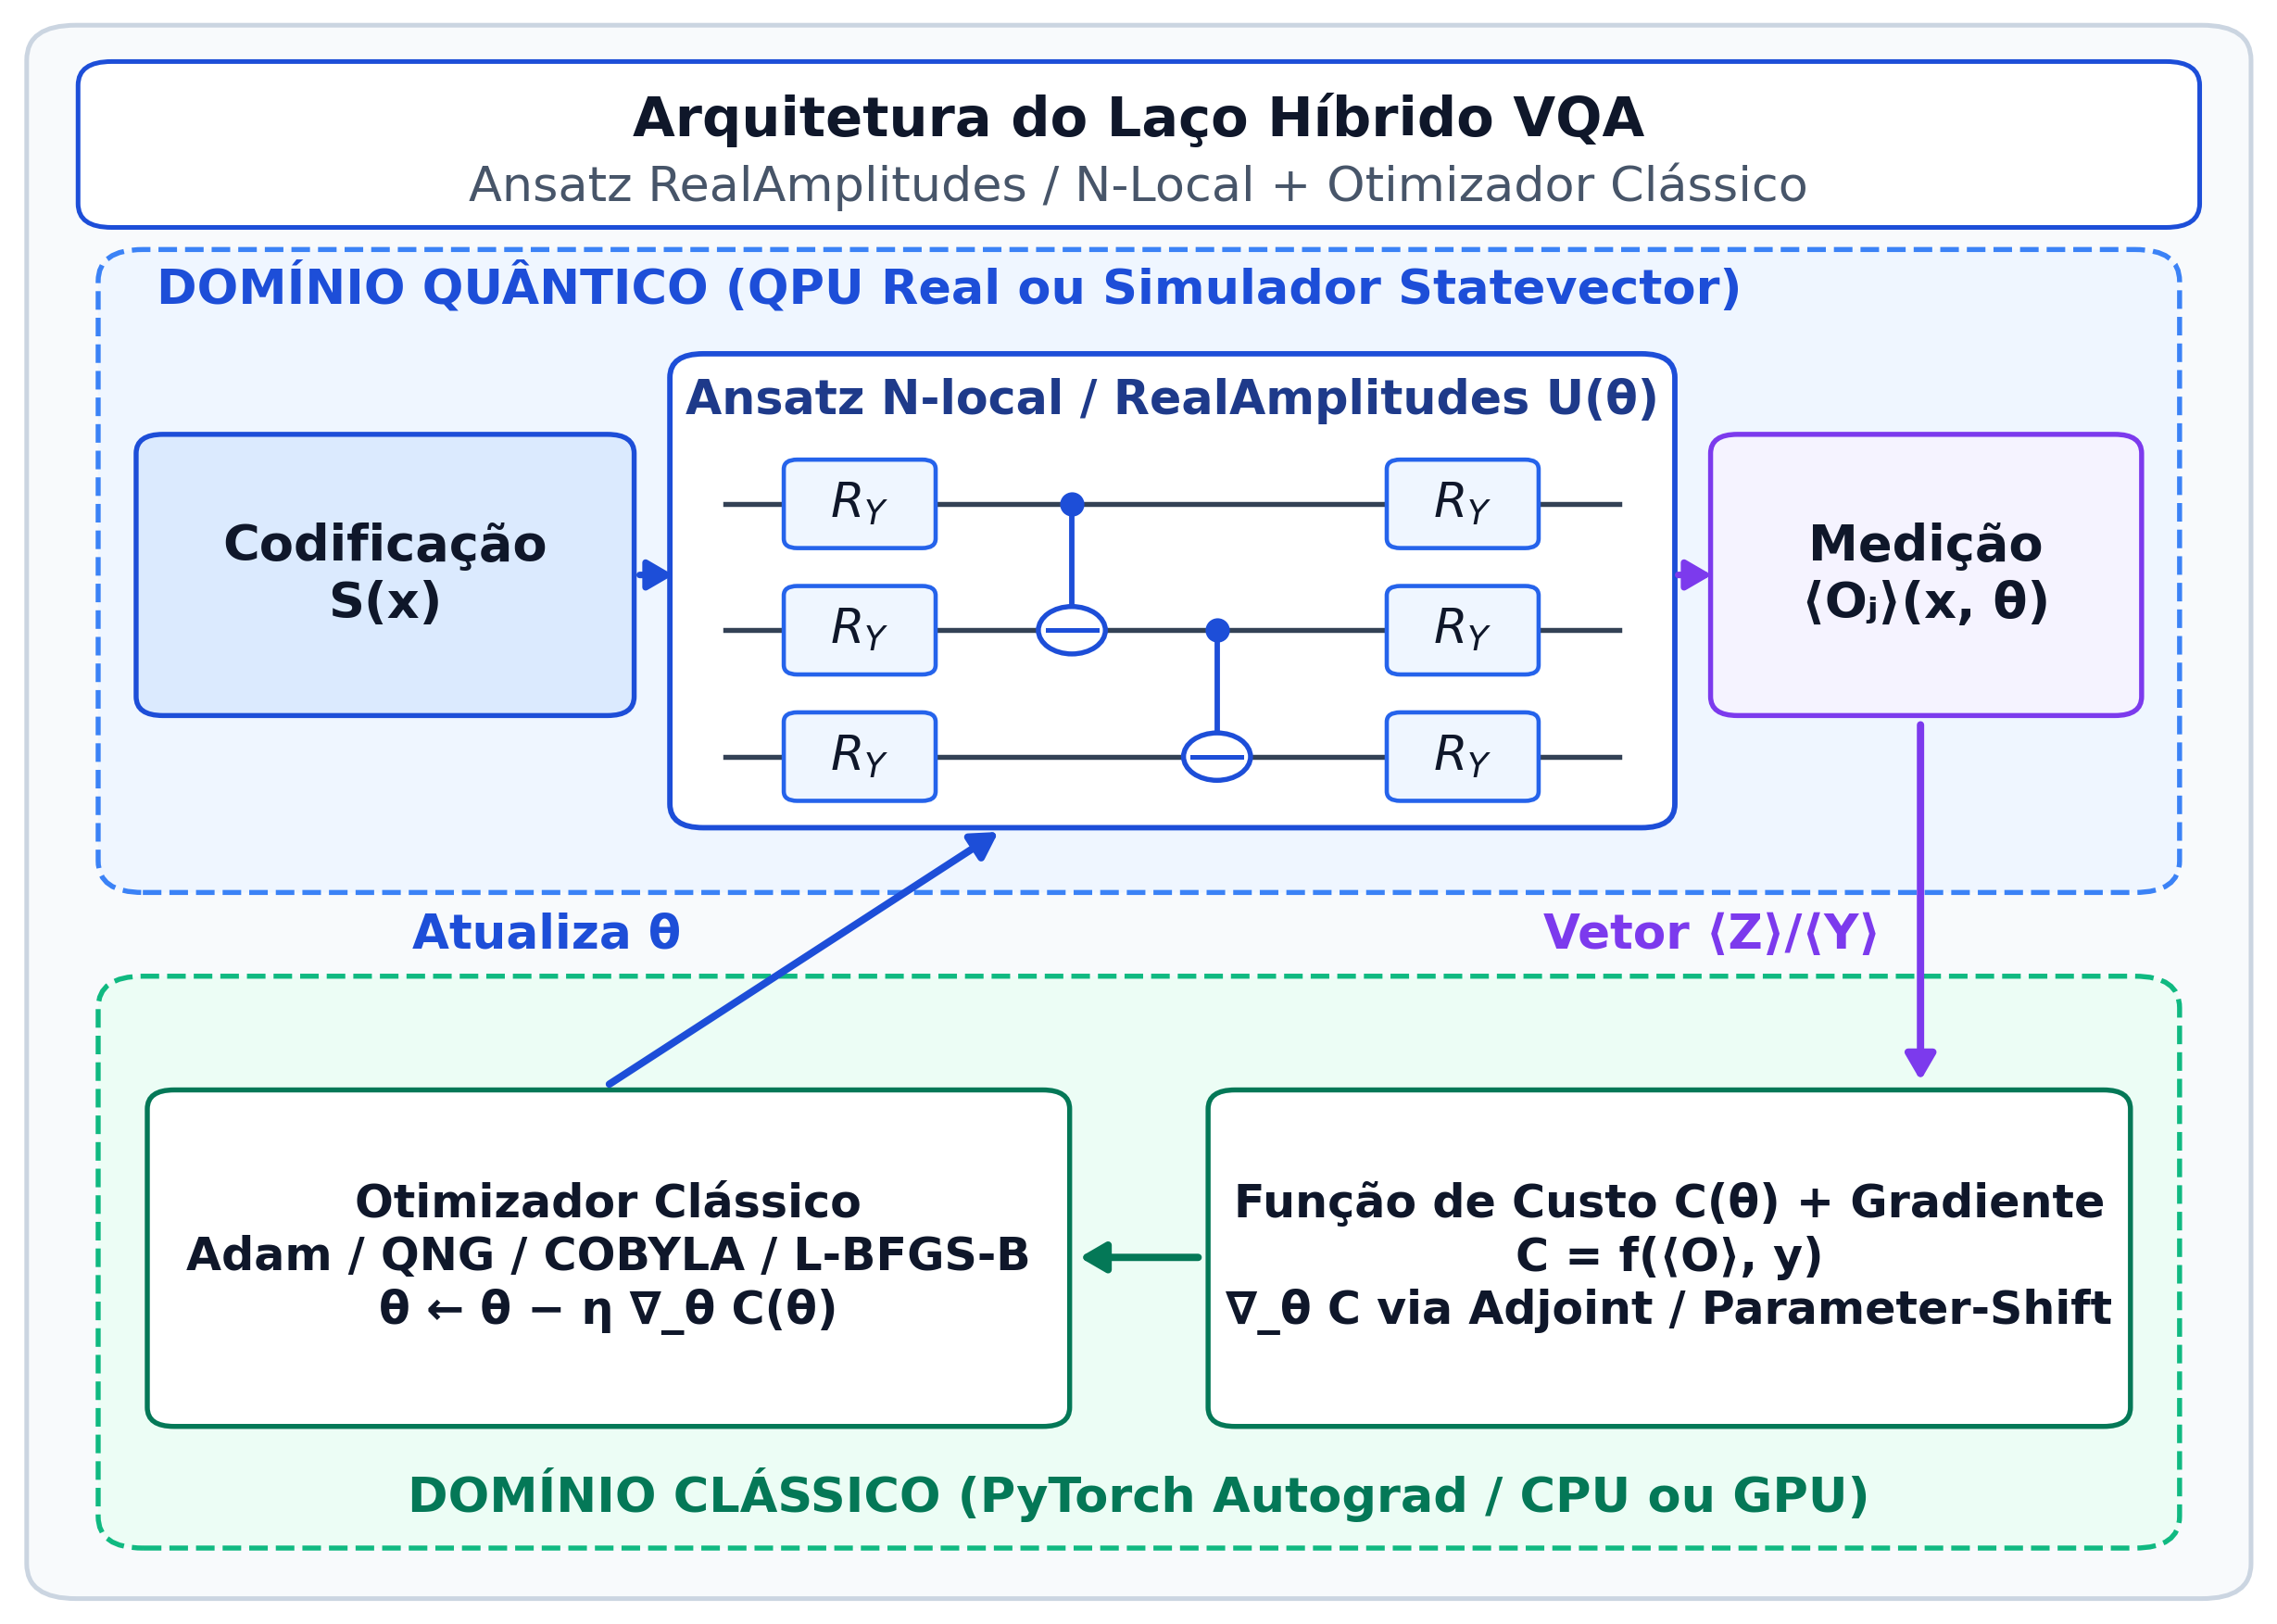
\includegraphics[width=\textwidth,height=0.46\textheight,keepaspectratio]{fig_264_laco_vqa.png}
    \end{column}
  \end{columns}
  \vspace{0.12cm}
  \begin{itemize}\footnotesize
    \item \textbf{Codificação angular:} vetor clássico vira ângulos de rotação $R_X$ nos qubits em profundidade $\mathcal{O}(1)$
    \item \textbf{Laço VQA:} \textit{ansatz} parametrizado atualizado por gradientes (\textit{parameter-shift}) acoplado ao otimizador clássico
  \end{itemize}
  \fonte{Elaborado pelo autor (2026), com base em Schuld, Sweke e Meyer (2021), Pérez-Salinas et al.\ (2020), Cerezo et al.\ (2021) e IBM Quantum (2026).}
\end{frame}

% 15 - SIMULAÇÃO, BARREN PLATEAUS E ESCALABILIDADE
\begin{frame}{Simulação, \textit{barren plateaus} e escalabilidade}
  \begin{columns}[T,onlytextwidth]
    \begin{column}{0.48\textwidth}
      \centering
      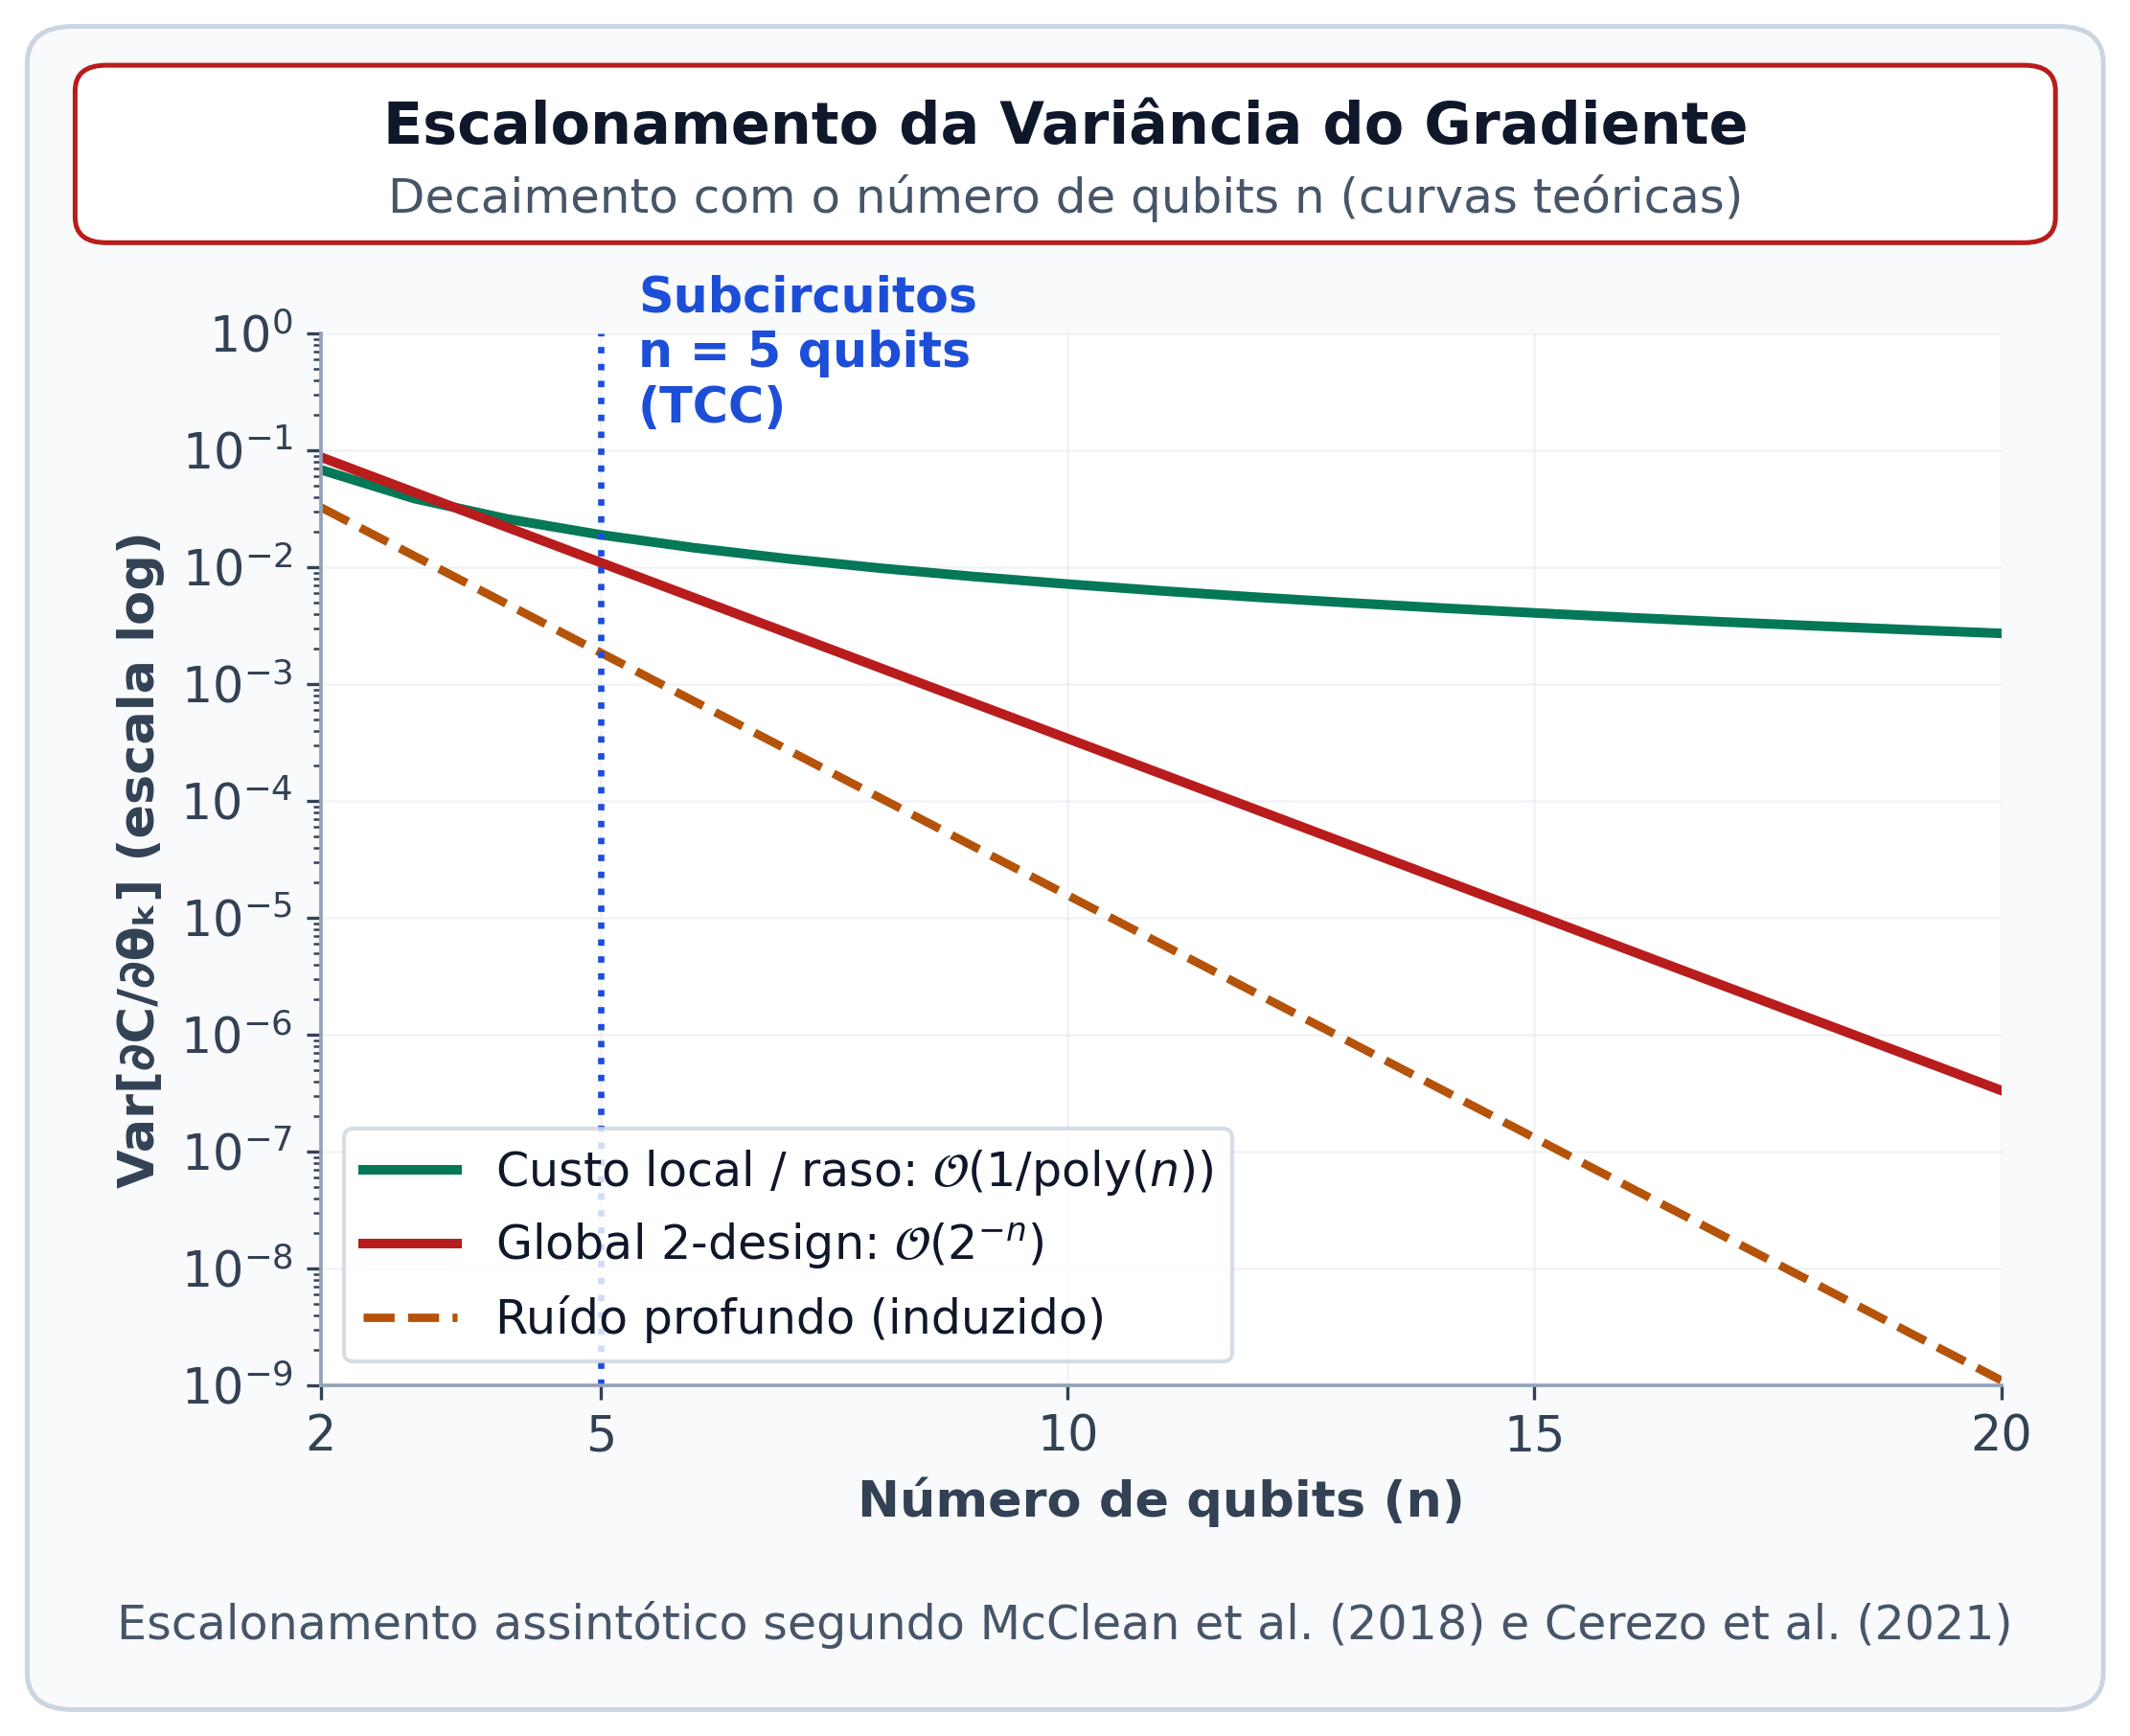
\includegraphics[width=\textwidth,height=0.46\textheight,keepaspectratio]{fig_265_variancia_gradiente.png}
    \end{column}
    \begin{column}{0.48\textwidth}
      \centering
      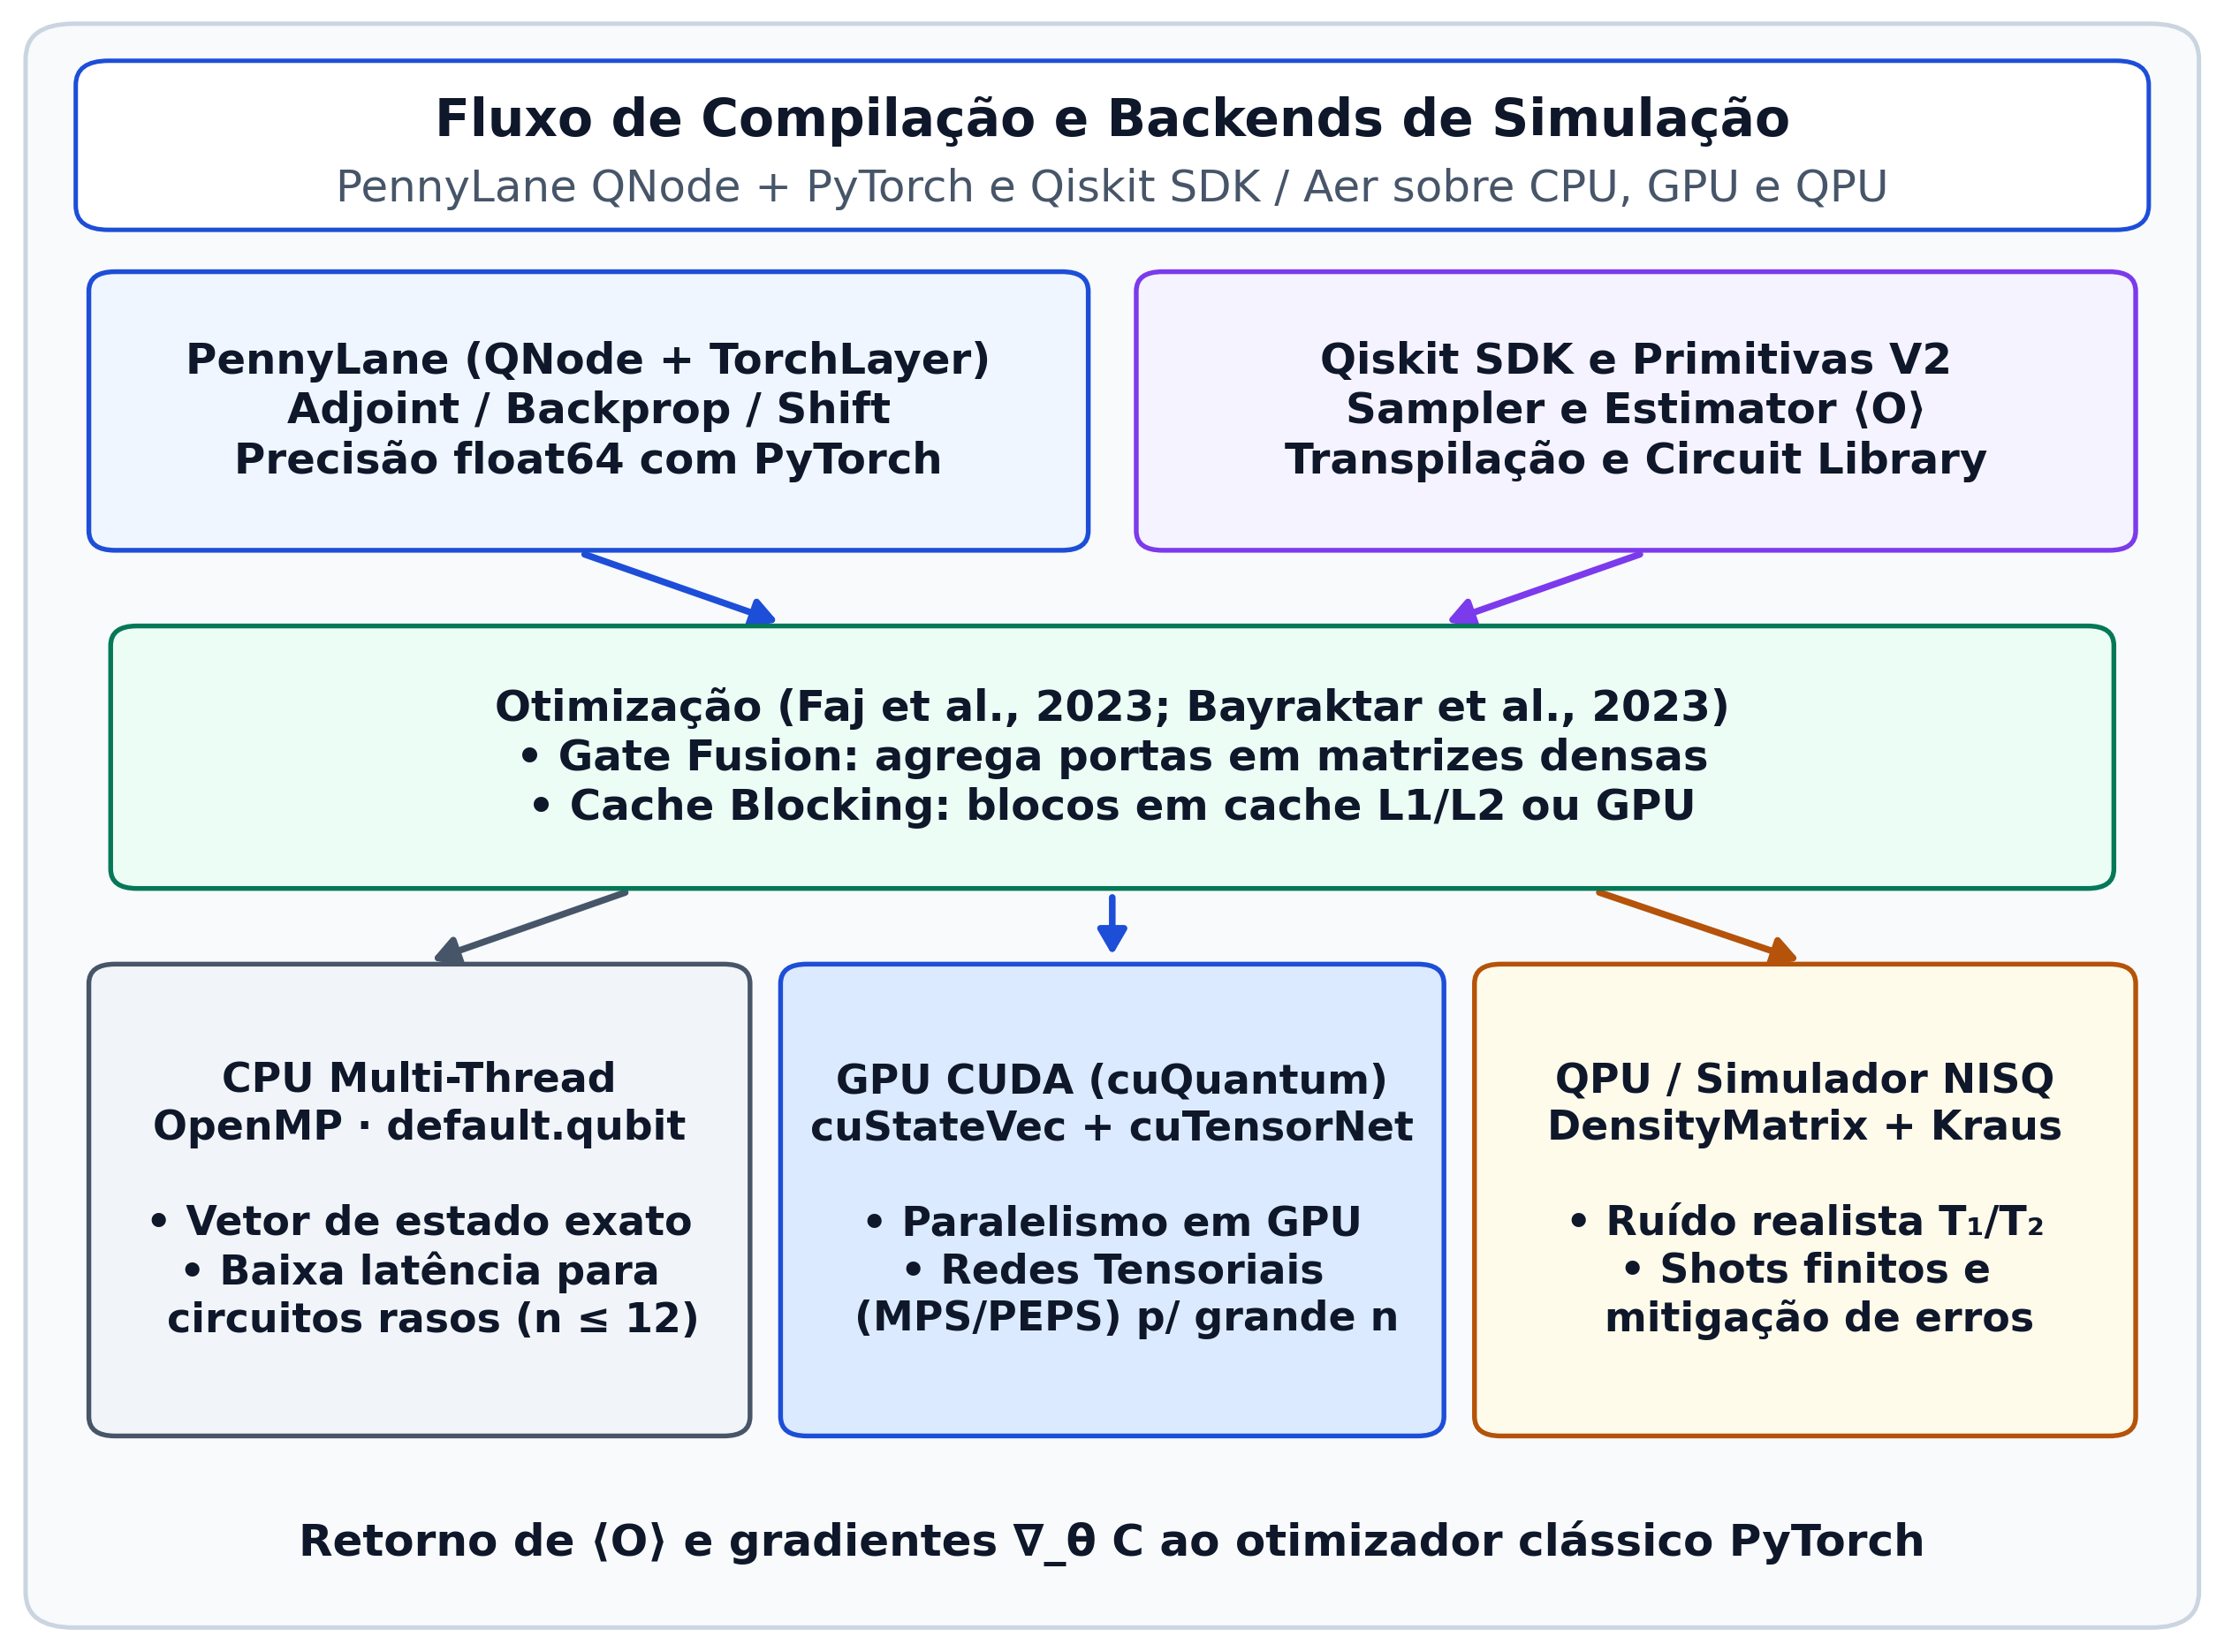
\includegraphics[width=\textwidth,height=0.46\textheight,keepaspectratio]{fig_266_fluxo_backends_simulacao.png}
    \end{column}
  \end{columns}
  \vspace{0.12cm}
  \begin{itemize}\footnotesize
    \item Simular 20 qubits em vetor de estado exige $2^{20}$ (1.048.576) amplitudes e sofre com \textit{barren plateaus}
    \item \textbf{Decisão arquitetural:} decompor em 4 circuitos paralelos de 5 qubits ($2^5 = 32$ estados cada)
  \end{itemize}
  \fonte{Elaborado pelo autor (2026), com base em McClean et al.\ (2018), Cerezo et al.\ (2021), Faj et al.\ (2023) e Bayraktar et al.\ (2023).}
\end{frame}

% 16 - MODELO DE REFERÊNCIA: HQNN-PARALLEL
\begin{frame}{Modelo de referência: HQNN-Parallel (Senokosov et al., 2024)}
  \centering
  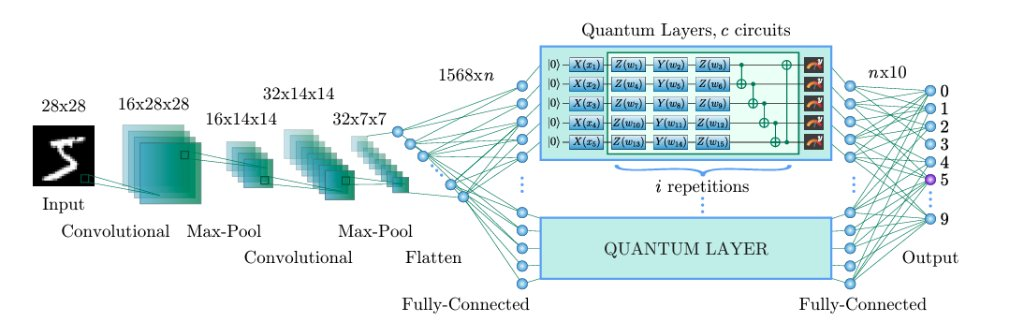
\includegraphics[width=0.90\textwidth,height=0.25\textheight,keepaspectratio]{fig_arxiv2304_hqnn_parallel_arquitetura.jpg}
  \vspace{0.04cm}
  \begin{columns}[T,onlytextwidth]
    \begin{column}{0.48\textwidth}
      \begin{block}{Circuito preservado ($4\times 5$ qubits)}
        \begin{itemize}\setlength{\itemsep}{2pt}
          \item Codificação $R_X$ + 3 camadas $R_Z$--$R_Y$--$R_Z$ com CNOT cíclico
          \item Medição Pauli-$Y$: 45 pesos/ramo = 180 quânticos
          \item MNIST: 99,21\% (45k pesos) vs.\ 98,71\% CNN (372k)
        \end{itemize}
      \end{block}
    \end{column}
    \begin{column}{0.48\textwidth}
      \begin{block}{Adaptações neste TCC}
        \begin{itemize}\setlength{\itemsep}{2pt}
          \item Extrator padronizado de 5 blocos congelado (\texttt{features128})
          \item Projeção clássica $128\to 20$ comum ao controle \texttt{Dense20}
          \item Execução cruzada: 9 bases, Macro-F1, PennyLane e Qiskit
        \end{itemize}
      \end{block}
    \end{column}
  \end{columns}
  \fonte{Extraído de Senokosov et al.\ (2024) (\texttt{arXiv:2304.09224}, Figura 4).}
\end{frame}

% 17 - REVISÃO DA LITERATURA (FUNIL)
\begin{frame}{Como foi a revisão da literatura}
  \begin{columns}[T,onlytextwidth]
    \begin{column}{0.52\textwidth}
      \centering
      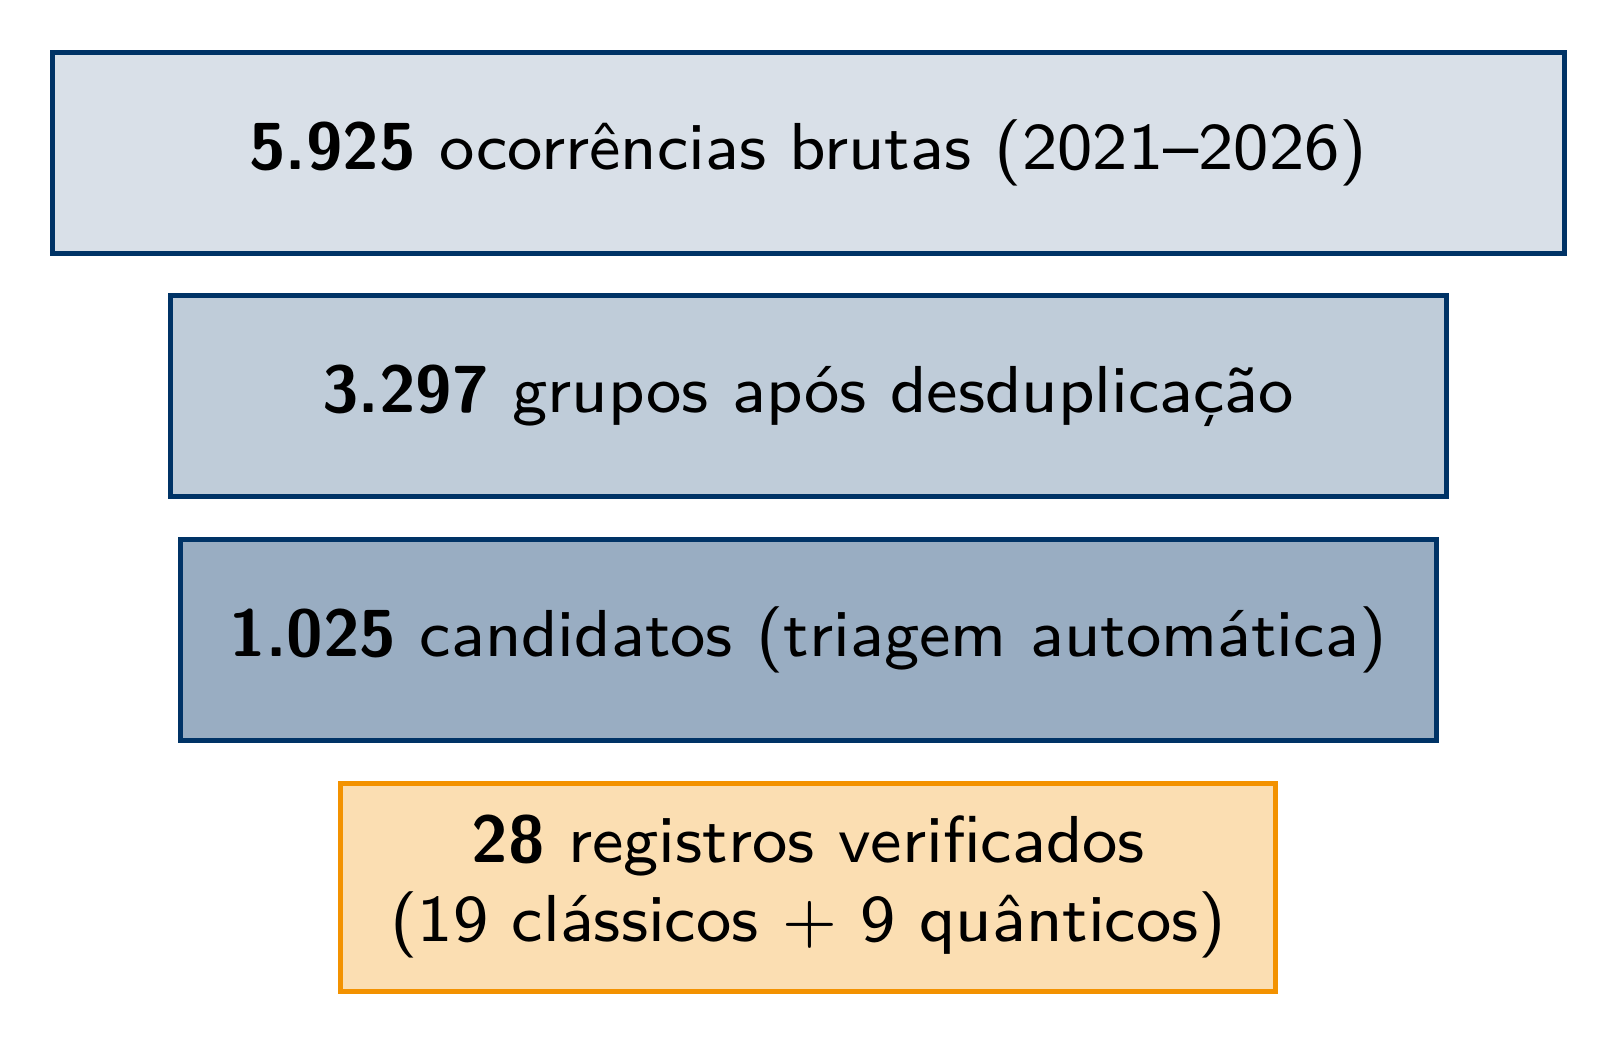
\includegraphics[width=\textwidth,height=0.66\textheight,keepaspectratio]{fig_funil_pesquisa.png}
    \end{column}
    \begin{column}{0.45\textwidth}
      \begin{block}{Diretrizes da auditoria bibliográfica}
        \begin{itemize}\setlength{\itemsep}{4pt}
          \item \textbf{Frente 1:} fundamentação teórica e artigos originais das 9 bases
          \item \textbf{Frente 2:} estudos empíricos por base (recorte 2021--2026)
          \item Conferência manual na fonte primária: variante, classes, partição e métrica
          \item 28 registros verificados (19 clássicos + 9 quânticos/híbridos)
        \end{itemize}
      \end{block}
    \end{column}
  \end{columns}
  \fonte{Elaborado pelo autor (2026).}
\end{frame}

% 18 - CORRELATOS CLÁSSICOS
\begin{frame}{Estudos clássicos nas nove bases}
  \centering
  {\footnotesize
  \begin{tabular}{@{}llr@{}}
    \toprule
    \textbf{Base} & \textbf{Estudo e arquitetura} & \textbf{Acurácia} \\
    \midrule
    MNIST & Kabir et al.\ (2023) --- VGG-5 + Spinal FC & 99,69\% \\
    Fashion-MNIST & Khanday et al.\ (2021) --- CNN rasa (filtro $3\times 3$) & 92,68\% \\
    KMNIST & Kabir et al.\ (2023) --- VGG-5 + Spinal FC & 99,05\% \\
    EMNIST Balanced & Kabir et al.\ (2023) --- VGG-5 + Spinal FC (47 cl.) & 90,73\% \\
    CIFAR-10 & Khanday et al.\ (2021) --- CNN $3\times 3$ (50 épocas) & 73,04\% \\
    CIFAR-100 Coarse & Guo et al.\ (2018) --- CNN-RNN (tarefa conjunta) & 88,23\% \\
    SVHN & Huang et al.\ (2017) --- DenseNet (c/ conj.\ extra) & 98,41\% \\
    GTSRB & An et al.\ (2024) --- LeNet-5 mod.\ (Tab.\ 8: \texttt{val\_acc}) & 97,53\% \\
    FER2013 & Li et al.\ (2021) --- Auto-FERNet (re-rotulagem) & 73,78\% \\
    \bottomrule
  \end{tabular}}
  \vspace{0.15cm}
  {\footnotesize\bfseries\color{senacblue}Acurácias dos artigos originais: não equivalem diretamente ao Macro-F1 deste TCC (protocolos distintos).}
  \fonte{Elaborado pelo autor (2026), a partir da auditoria das publicações originais.}
\end{frame}

% 19 - CORRELATOS QUÂNTICOS E HÍBRIDOS
\begin{frame}{Estudos quânticos e híbridos na literatura}
  \centering
  {\footnotesize
  \begin{tabular}{@{}lR{10.5cm}@{}}
    \toprule
    \textbf{Base} & \textbf{Recorte e resultado reportado na literatura} \\
    \midrule
    MNIST & Binário 3 vs.\ 5: 98,85\% (Long, 2025); 10 cl.\ NNQE: 93,8\% (Riaz, 2023) \\
    Fashion-MNIST & 4 classes: 85,9--93,6\% vs.\ 89,7--97,4\% CNN (Bokhan, 2022) \\
    KMNIST & Apenas experimento binário confirmado (Dong, 2025) \\
    EMNIST & 75,9\% com filtro quântico fixo de 4 qubits (Riaz, 2026) \\
    CIFAR-10 & NNQE cinza: 36,0\% teste (Riaz, 2023); HQNN: 82,78\% (Senokosov, 2024) \\
    \textbf{CIFAR-100 Coarse} & \textbf{Nenhum estudo quântico/híbrido confirmado nas 20 superclasses} \\
    GTSRB & NNQE: 73,4\% vs.\ 82,2\% na rede densa clássica (Riaz, 2023) \\
    \bottomrule
  \end{tabular}}
  \vspace{0.18cm}
  {\footnotesize\bfseries\color{senacorange}Predominam recortes binários/4 classes e filtros fixos; no GTSRB, NNQE perde em 8,8 p.p.\ para a rede clássica.}
  \fonte{Elaborado pelo autor (2026), a partir da auditoria das publicações originais.}
\end{frame}

% 20 - LACUNA DE PESQUISA
\begin{frame}{Lacuna de pesquisa}
  \small
  \begin{enumerate}\setlength{\itemsep}{6pt}
    \item \textbf{Protocolos fragmentados:} poucas classes ou domínios; lacuna aberta nas 20 superclasses do CIFAR-100 Coarse
    \item \textbf{Omissão do Macro-F1:} literatura reporta quase só acurácia global, mascarando minoritárias (GTSRB, FER2013, SVHN)
    \item \textbf{Variáveis de confusão:} lotes assimétricos (ex.: 1 vs.\ 4) e falta de controle clássico com gargalo de mesma dimensão
  \end{enumerate}
  \vspace{0.25cm}
  \begin{block}{Contribuição proposta}
    Campanha padronizada nas 9 bases completas (72 modelos), avaliada por Macro-F1 com controle vetorial \texttt{Dense20}, calibração, oclusão $8\times 8$ e telemetria multiplataforma.
  \end{block}
\end{frame}

% 21 - TIPO DE PESQUISA E PERGUNTA
\begin{frame}{Tipo de pesquisa e pergunta norteadora}
  \small
  \begin{itemize}\setlength{\itemsep}{6pt}
    \item \textbf{Natureza aplicada}, abordagem \textbf{quantitativa} e protocolo estritamente auditável
    \item Objetivos \textbf{exploratórios} (CIFAR-100 Coarse e EMNIST), \textbf{descritivos} (72 modelos + 36 balanceamento + 27 telemetria M4) e \textbf{comparativos}
  \end{itemize}
  \vspace{0.25cm}
  \begin{block}{Pergunta de pesquisa}
    Em que medida uma representação convolucional congelada (\texttt{features128}) sustenta cabeças reduzidas nas nove bases, e como a cabeça híbrida ($4\times 5$ qubits) se compara em Macro-F1, calibração, explicabilidade e custo frente à CNN original e ao controle \texttt{Dense20}?
  \end{block}
\end{frame}

% 22 - PIPELINE EXPERIMENTAL
\begin{frame}{Pipeline experimental em seis etapas}
  \centering
  \vspace{0.15cm}
  \begin{tikzpicture}[node distance=0.55cm and 0.45cm,>=Stealth]
    \node[stagebox] (e1) {\textbf{1. Inventário e dados}\\9 bases 70/15/15\\Hashes SHA-256};
    \node[stagebox,right=of e1] (e2) {\textbf{2. Extrator FP32}\\CNN $64\times 64$ ($128\times 128$)\\Exporta \texttt{features128}};
    \node[stagebox,right=of e2] (e3) {\textbf{3. Cabeças Dense20}\\D20 imagem e vetorial\\(Linux e macOS)};
    \node[stagebox,below=1.0cm of e1] (e4) {\textbf{4. Híbrido $4\times 5$ qubits}\\36 treinos em CPU\\Win/Mac $\times$ PL/Qiskit};
    \node[stagebox,right=of e4] (e5) {\textbf{5. Auditoria completa}\\Macro-F1, Bayes, ECE\\Grad-CAM e oclusão};
    \node[stagebox,right=of e5] (e6) {\textbf{6. Telemetria}\\Tempos lote 128, CPU\\RSS, GPU, I/O e \texttt{macmon}};
    \draw[->,thick,senacorange] (e1)--(e2);
    \draw[->,thick,senacorange] (e2)--(e3);
    \draw[->,thick,senacorange] (e3.south)--++(0,-0.48)-|(e4.north);
    \draw[->,thick,senacorange] (e4)--(e5);
    \draw[->,thick,senacorange] (e5)--(e6);
  \end{tikzpicture}
  \fonte{Elaborado pelo autor (2026).}
\end{frame}

% 23 - AS NOVE BASES DE DADOS
\begin{frame}{As nove bases de dados}
  \centering
  {\footnotesize
  \begin{tabular}{@{}lllrr@{}}
    \toprule
    \textbf{Base} & \textbf{Domínio} & \textbf{Entrada} & \textbf{K} & \textbf{Treino / Val.\ / Teste} \\
    \midrule
    MNIST & Dígitos manuscritos & $28\times 28$, cinza & 10 & 48.999 / 10.503 / 10.498 \\
    Fashion-MNIST & Vestuário & $28\times 28$, cinza & 10 & 49.000 / 10.500 / 10.500 \\
    KMNIST & Caracteres Kuzushiji & $28\times 28$, cinza & 10 & 49.000 / 10.500 / 10.500 \\
    EMNIST Balanced & Alfanumérico & $28\times 28$, cinza & 47 & 92.120 / 19.740 / 19.740 \\
    CIFAR-10 & Objetos e animais & $32\times 32$, RGB & 10 & 42.000 / 9.000 / 9.000 \\
    CIFAR-100 Coarse & Superclasses & $32\times 32$, RGB & 20 & 42.000 / 9.000 / 9.000 \\
    SVHN & Dígitos de fachadas & $32\times 32$, RGB & 10 & 69.502 / 14.894 / 14.893 \\
    GTSRB & Placas de trânsito & Variável, RGB & 43 & 27.489 / 5.905 / 5.876 \\
    FER2013 & Expressões faciais & $48\times 48$, cinza & 7 & 25.121 / 5.384 / 5.382 \\
    \bottomrule
  \end{tabular}}
  \vspace{0.15cm}
  {\footnotesize\color{textmuted}Partições estratificadas fixas (70/15/15) compartilhadas pelos 8 modelos em cada base.}
  \fonte{Elaborado pelo autor (2026).}
\end{frame}

% 24 - EQUILÍBRIO DE CLASSES
\begin{frame}{Equilíbrio de classes: três regimes}
  \begin{columns}[T,onlytextwidth]
    \begin{column}{0.49\textwidth}
      \centering
      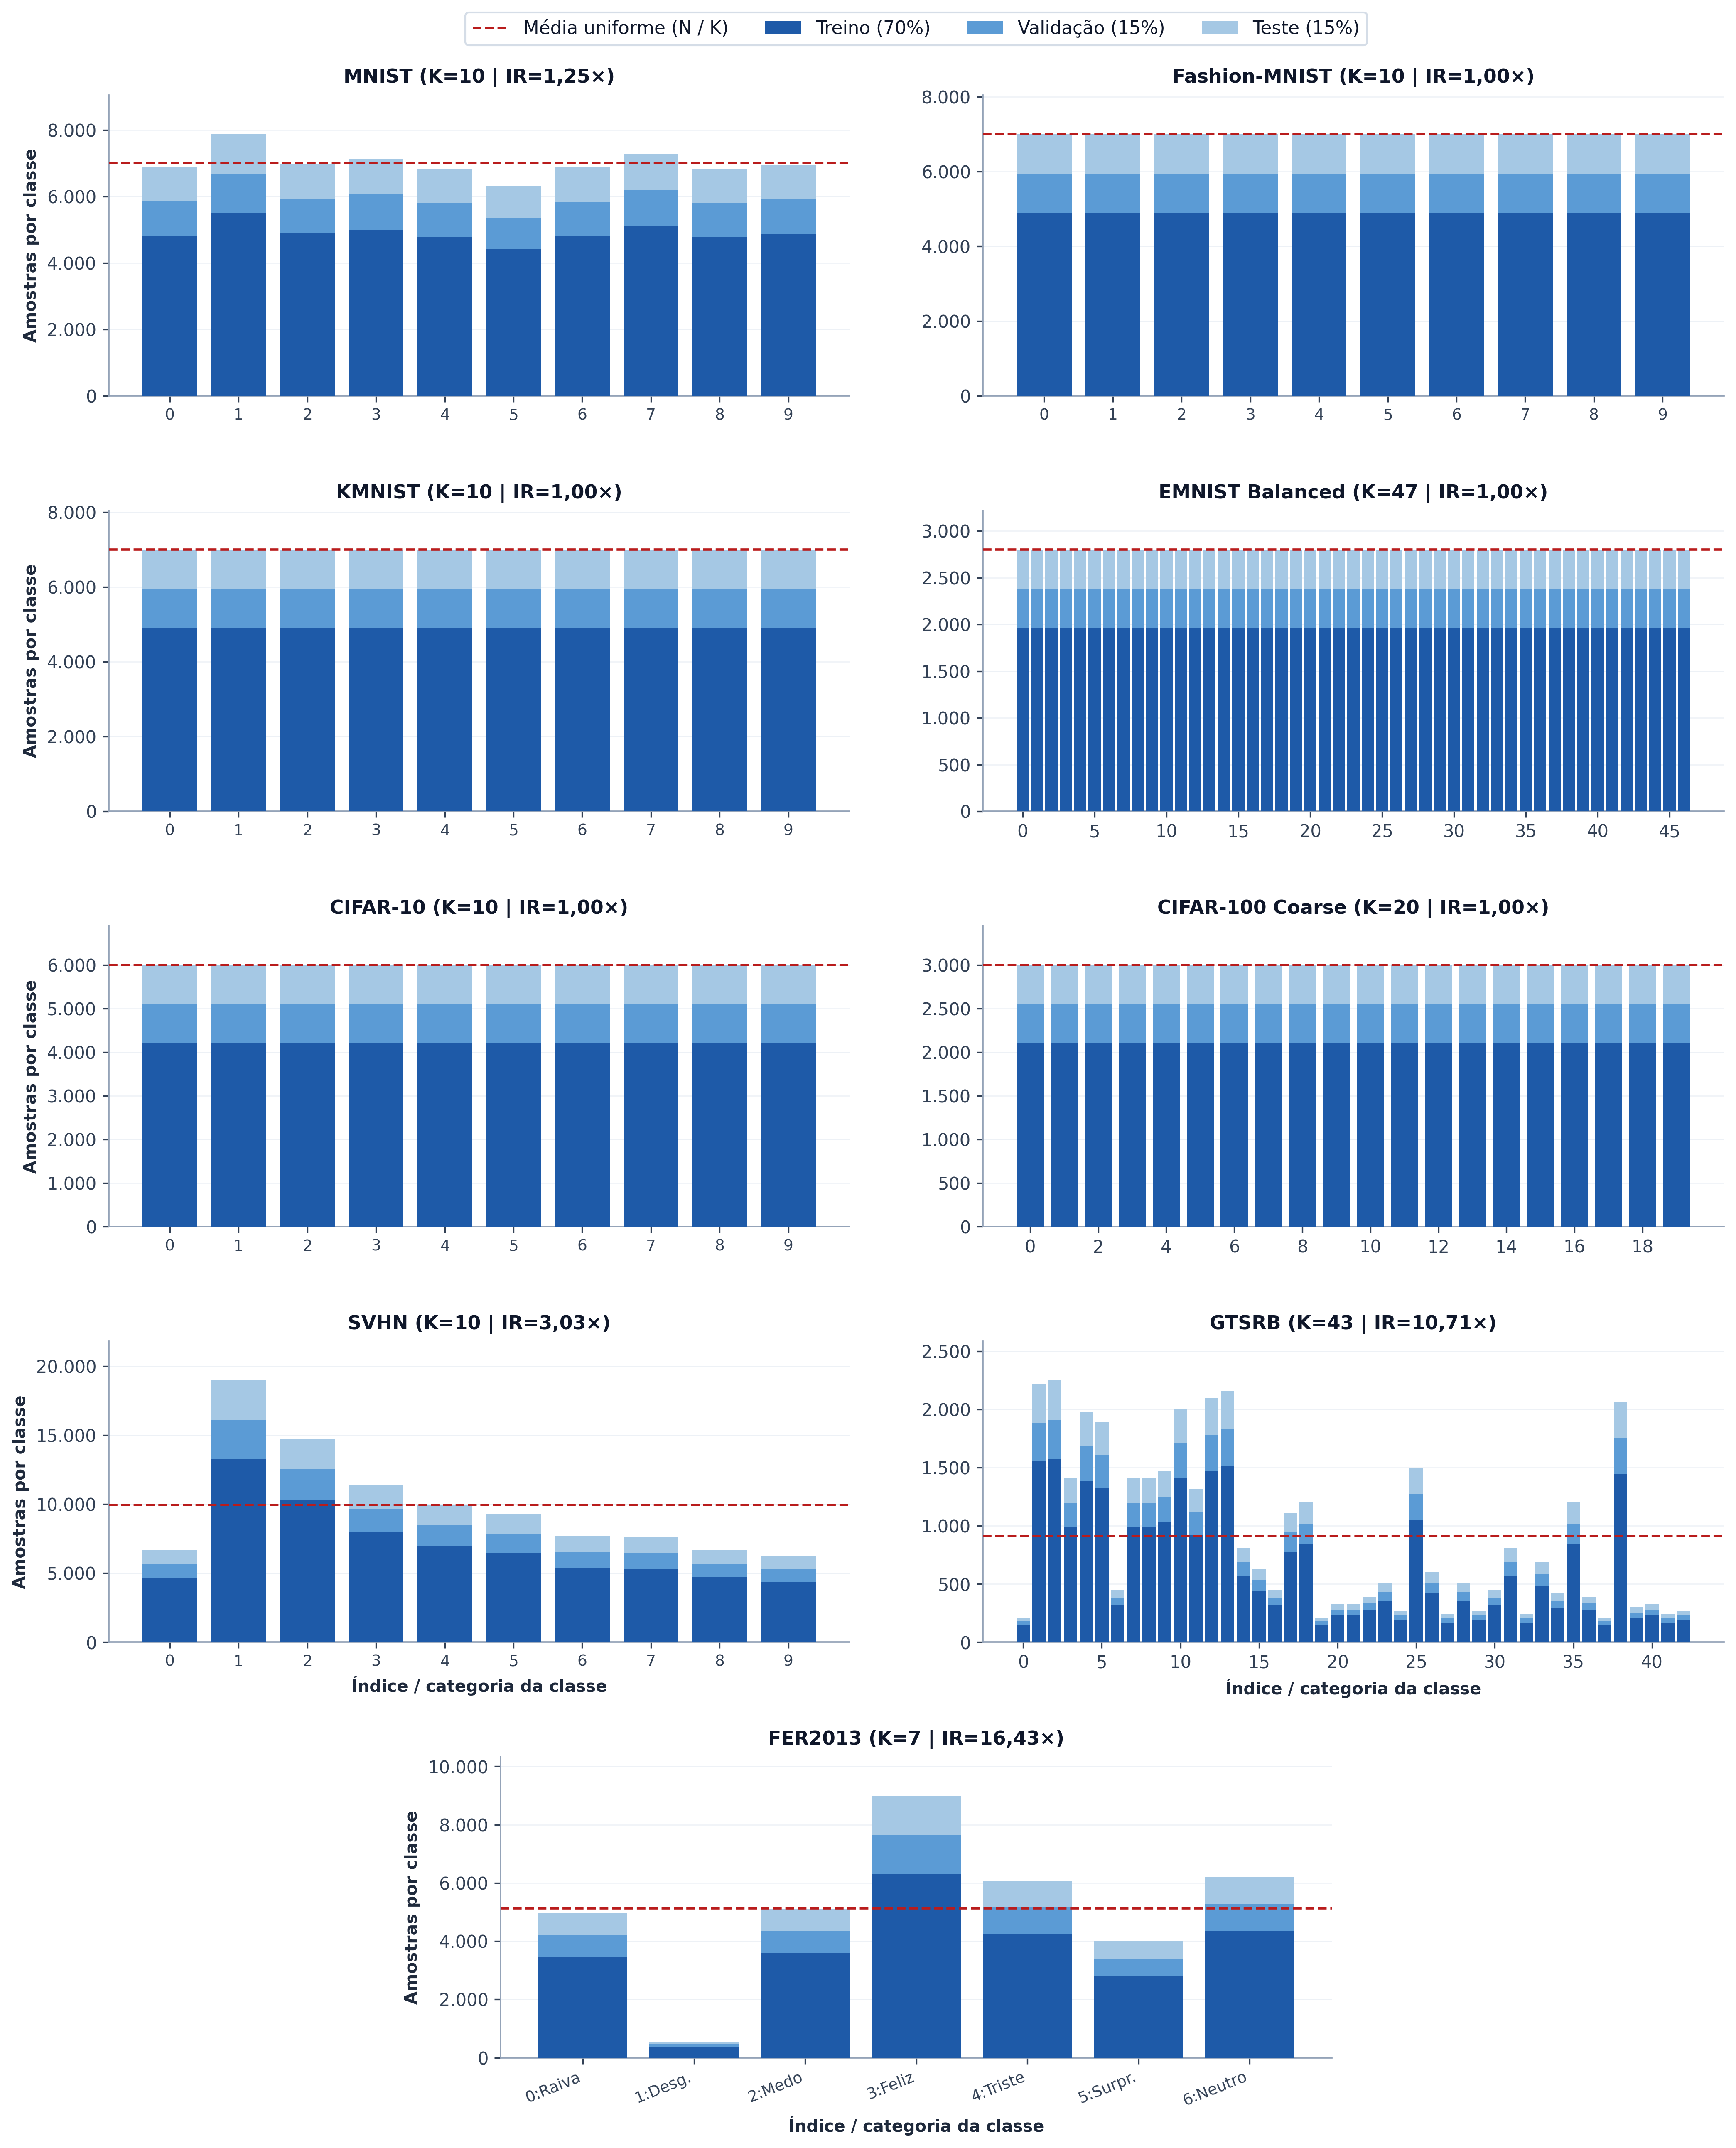
\includegraphics[trim=0pt 498bp 0pt 0pt,clip,width=\textwidth,height=0.69\textheight,keepaspectratio]{equilibrio_classes_9_datasets.png}
    \end{column}
    \begin{column}{0.49\textwidth}
      \centering
      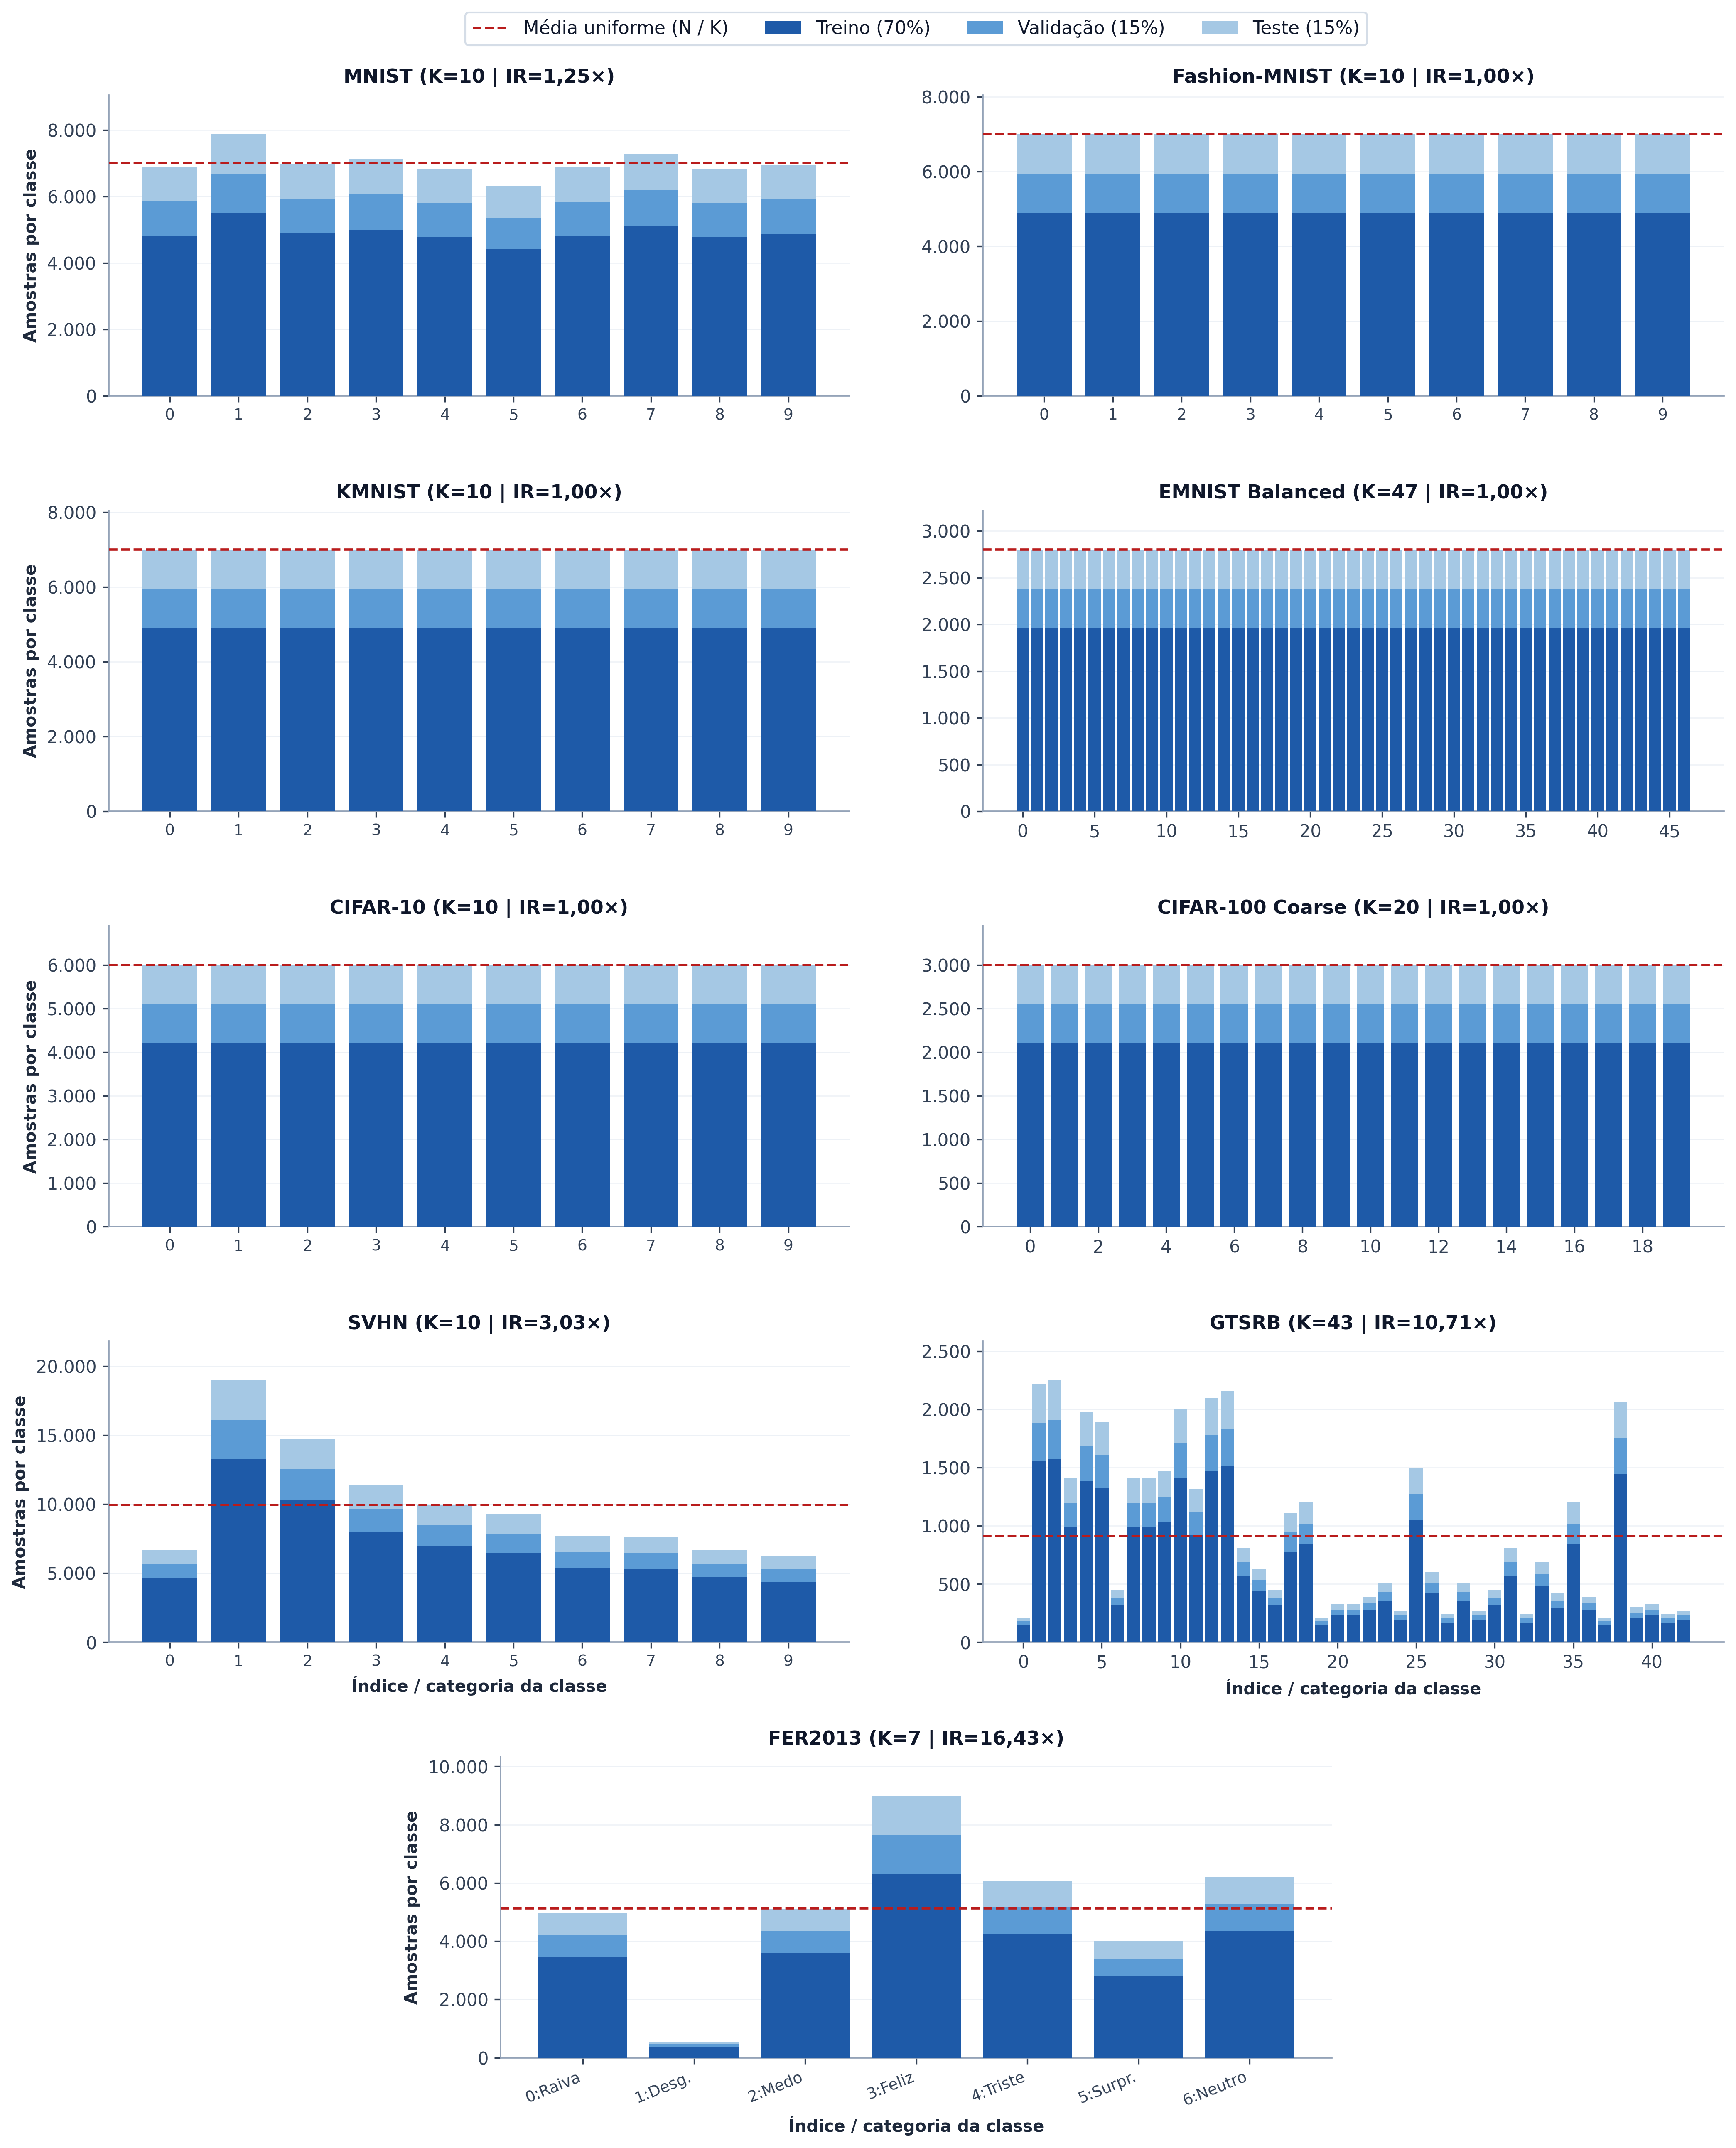
\includegraphics[trim=0pt 0pt 0pt 743bp,clip,width=\textwidth,height=0.29\textheight,keepaspectratio]{equilibrio_classes_9_datasets.png}\par\vspace{0.04cm}
      \begin{block}{Regimes ($\text{IR} = n_{\max}/n_{\min}$)}
        {\scriptsize
        \begin{itemize}\setlength{\itemsep}{1pt}
          \item \textbf{IR $= 1{,}00\times$ (CV $= 0\%$):} Fashion, KMNIST, EMNIST, CIFAR-10 e CIFAR-100 Coarse
          \item \textbf{IR $= 1{,}25\times$:} MNIST (assimetria branda)
          \item \textcolor{badred}{\textbf{IR $= 3{,}03\times$ a $16{,}43\times$:}} SVHN ($3{,}03\times$), GTSRB ($10{,}71\times$) e FER2013 ($16{,}43\times$; 547 desgosto)
          \item Validação e teste mantêm distribuição natural
        \end{itemize}}
      \end{block}
    \end{column}
  \end{columns}
  \fonte{Elaborado pelo autor (2026).}
\end{frame}

% 25 - MODOS DE BALANCEAMENTO: GRÁFICOS
\begin{frame}{Modos de balanceamento: Macro-F1 e tempo (36 execuções)}
  \begin{columns}[T,onlytextwidth]
    \begin{column}{0.53\textwidth}
      \centering
      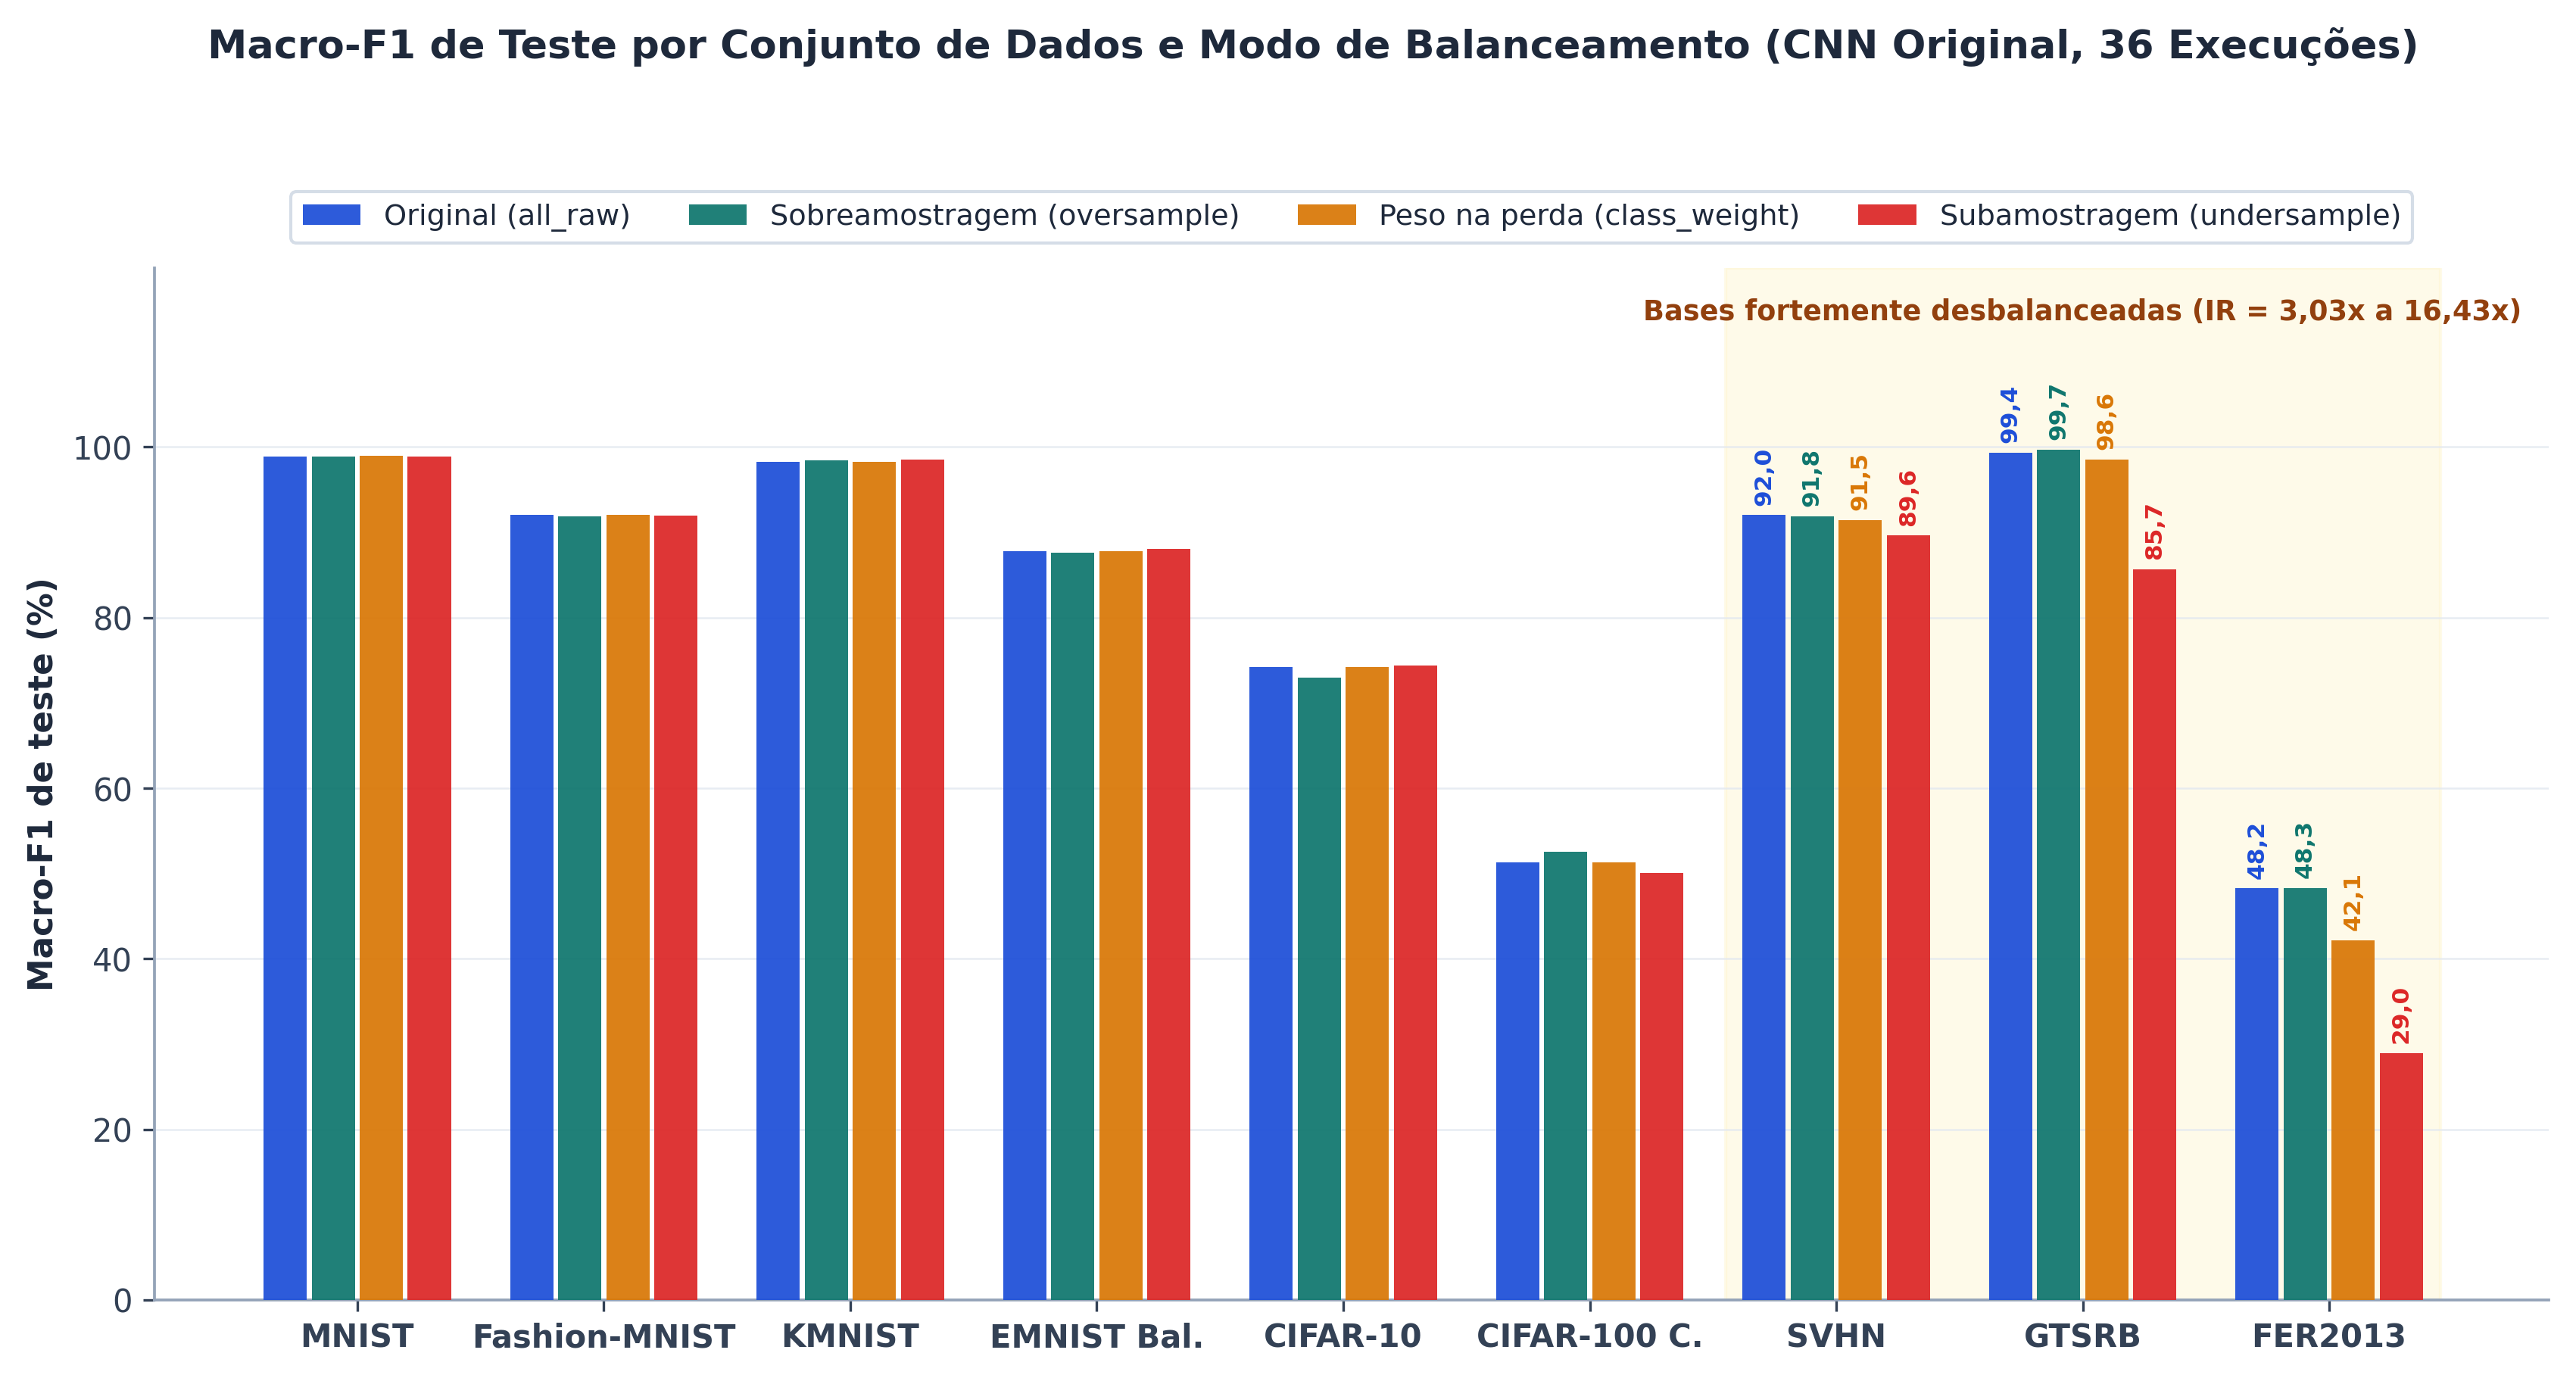
\includegraphics[width=\textwidth,height=0.56\textheight,keepaspectratio]{fig_balanceamento_macro_f1.png}
    \end{column}
    \begin{column}{0.45\textwidth}
      \centering
      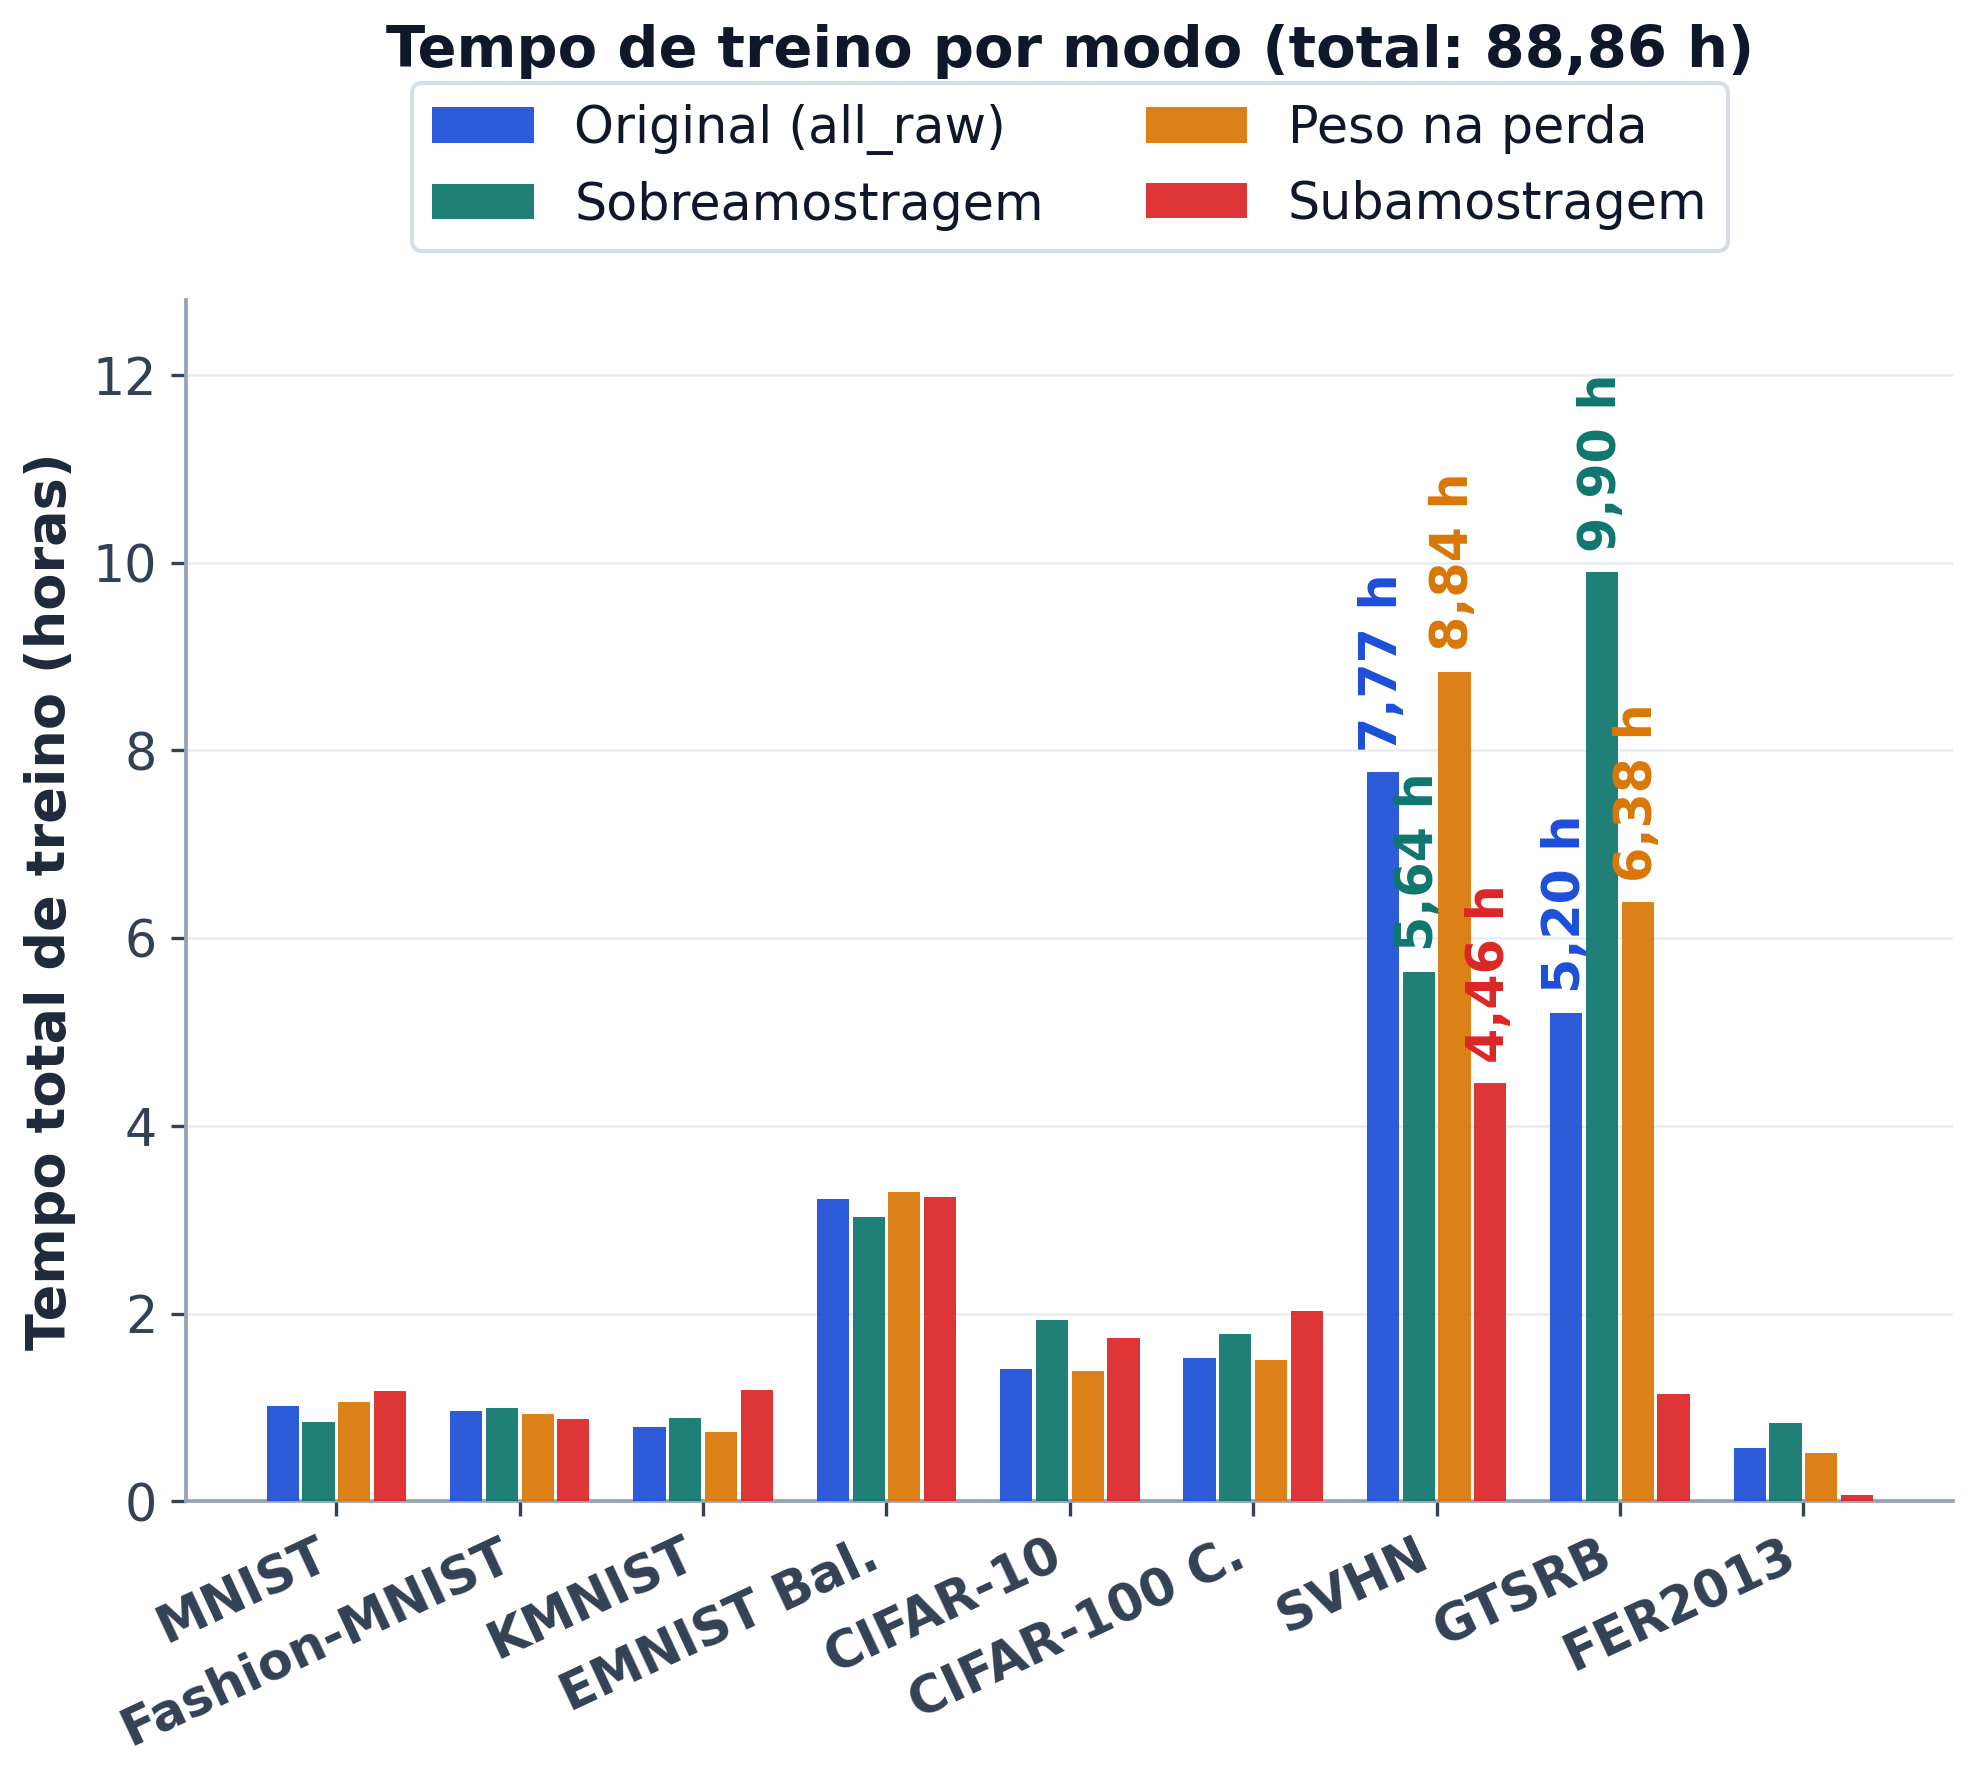
\includegraphics[width=\textwidth,height=0.56\textheight,keepaspectratio]{fig_342_balanceamento_tempo_treino.png}
    \end{column}
  \end{columns}
  \vspace{0.15cm}
  \centering
  {\footnotesize\bfseries\color{senacblue}Triagem preliminar na CNN original (\texttt{mixed\_float16}, lote 512, 2.486 épocas, 88,86 h acumuladas).}
  \fonte{Elaborado pelo autor (2026).}
\end{frame}

% 26 - JUSTIFICATIVA OBJETIVA DE all_raw
\begin{frame}{Por que adotar a distribuição natural (\texttt{all\_raw})?}
  \centering
  {\footnotesize
  \begin{tabular}{@{}lrrrr@{}}
    \toprule
    \textbf{Modo} & \textbf{Média Macro-F1} & \textbf{Mediana} & \textbf{$\Delta$ vs.\ \texttt{all\_raw}} & \textbf{Tempo total} \\
    \midrule
    \textbf{\texttt{all\_raw}} & \textbf{82,464\%} & \textbf{92,010\%} & \textbf{0,000 p.p.} & \textbf{22,46 h} \\
    \texttt{oversample} & 82,455\% & 91,851\% & $-0{,}009$ p.p. & 25,85 h \\
    \texttt{class\_weight} & 81,646\% & 91,467\% & $-0{,}819$ p.p. & 24,64 h \\
    \texttt{undersample} & 78,469\% & 88,057\% & $-3{,}995$ p.p. & 15,90 h \\
    \bottomrule
  \end{tabular}}
  \vspace{0.18cm}
  \begin{block}{Conclusão da triagem de 36 execuções}
    \begin{itemize}\setlength{\itemsep}{2pt}
      \item \textcolor{okgreen}{\textbf{\texttt{all\_raw}:}} maior média e mediana sem distorcer frequências nem custos quânticos
      \item \textcolor{badred}{\textbf{\texttt{undersample}:}} colapso severo em FER2013 ($-19{,}28$ p.p.) e GTSRB ($-13{,}69$ p.p.)
      \item \textcolor{badred}{\textbf{\texttt{class\_weight}:}} $-6{,}12$ p.p.\ no FER2013; idêntico a \texttt{all\_raw} nas 5 bases equilibradas
      \item \destaque{\texttt{oversample}:} $+15{,}1\%$ de tempo (GTSRB 9,90 h vs.\ 5,20 h) e $-1{,}26$ p.p.\ no CIFAR-10
    \end{itemize}
  \end{block}
  \fonte{Elaborado pelo autor (2026).}
\end{frame}

% 27 - PRÉ-PROCESSAMENTO E AUDITORIA DE INTEGRIDADE
\begin{frame}{Pré-processamento e auditoria de integridade}
  \begin{columns}[T,onlytextwidth]
    \begin{column}{0.48\textwidth}
      \begin{block}{Padronização idêntica}
        \begin{itemize}\setlength{\itemsep}{4pt}
          \item Tensores em ponto flutuante, normalização por canal e política \texttt{all\_raw}
          \item Redimensionamento proporcional (\texttt{resize\_with\_pad}) para $64\times 64$ ($128\times 128$ no GTSRB)
          \item Partição estratificada fixa (70/15/15) compartilhada pelos 8 modelos
          \item Rastreabilidade por hashes SHA-256
        \end{itemize}
      \end{block}
    \end{column}
    \begin{column}{0.48\textwidth}
      \begin{alertblock}{Limitações auditadas nos dados}
        \begin{itemize}\setlength{\itemsep}{5pt}
          \item \textcolor{badred}{\textbf{GTSRB:}} 3.990 de 5.876 imagens de teste (67,9\%) compartilham \textit{tracks} físicos com o treino
          \item \textcolor{badred}{\textbf{FER2013:}} 378 duplicatas exatas no teste (7,02\%), 403 na validação e 57 conflitos de rótulo
          \item EMNIST (1) e CIFAR-100 Coarse (7): cópias pontuais; 5 bases restantes livres de duplicatas
        \end{itemize}
      \end{alertblock}
    \end{column}
  \end{columns}
\end{frame}

% 28 - TRÊS FAMÍLIAS DE MODELOS
\begin{frame}{Três famílias de modelos comparadas}
  \begin{columns}[T,onlytextwidth]
    \begin{column}{0.32\textwidth}
      \begin{block}{CNN original (FP32)}
        5 blocos \texttt{SeparableConv2D} ($32\to 128$), GroupNorm(16), SiLU e MaxPool. Cabeça GAP+GMP $\to 256\to 256\to K$.\par\vspace{4pt}
        \textbf{Extrator:} 66.905 ($C=1$) ou 67.019 ($C=3$) pesos.
      \end{block}
    \end{column}
    \begin{column}{0.32\textwidth}
      \begin{block}{\texttt{Dense20} (controle)}
        Extrator congelado (\texttt{features128}): D20 imagem (LayerNorm+ReLU) e \texttt{Dense20} vetorial ($128\to 20\,\tanh\to K$).\par\vspace{4pt}
        \textbf{Função:} isolar o efeito do gargalo de 20 dimensões.
      \end{block}
    \end{column}
    \begin{column}{0.32\textwidth}
      \begin{block}{Híbrido $4\times 5$ qubits}
        Mesma projeção $128\to 20$ sobre \texttt{features128}; troca apenas $\tanh$ por 4 PQCs de 5 qubits.\par\vspace{4pt}
        Simulação exata em CPU: PennyLane e Qiskit Aer (Win e Mac).
      \end{block}
    \end{column}
  \end{columns}
  \vspace{0.35cm}
  \centering
  {\normalsize\bfseries\color{senacblue}Campanha principal auditada: 72 checkpoints = 9 bases $\times$ 8 configurações}
\end{frame}

% 29 - ETAPA 1: CNN ORIGINAL
\begin{frame}{Etapa 1: CNN clássica de origem (FP32)}
  \centering
  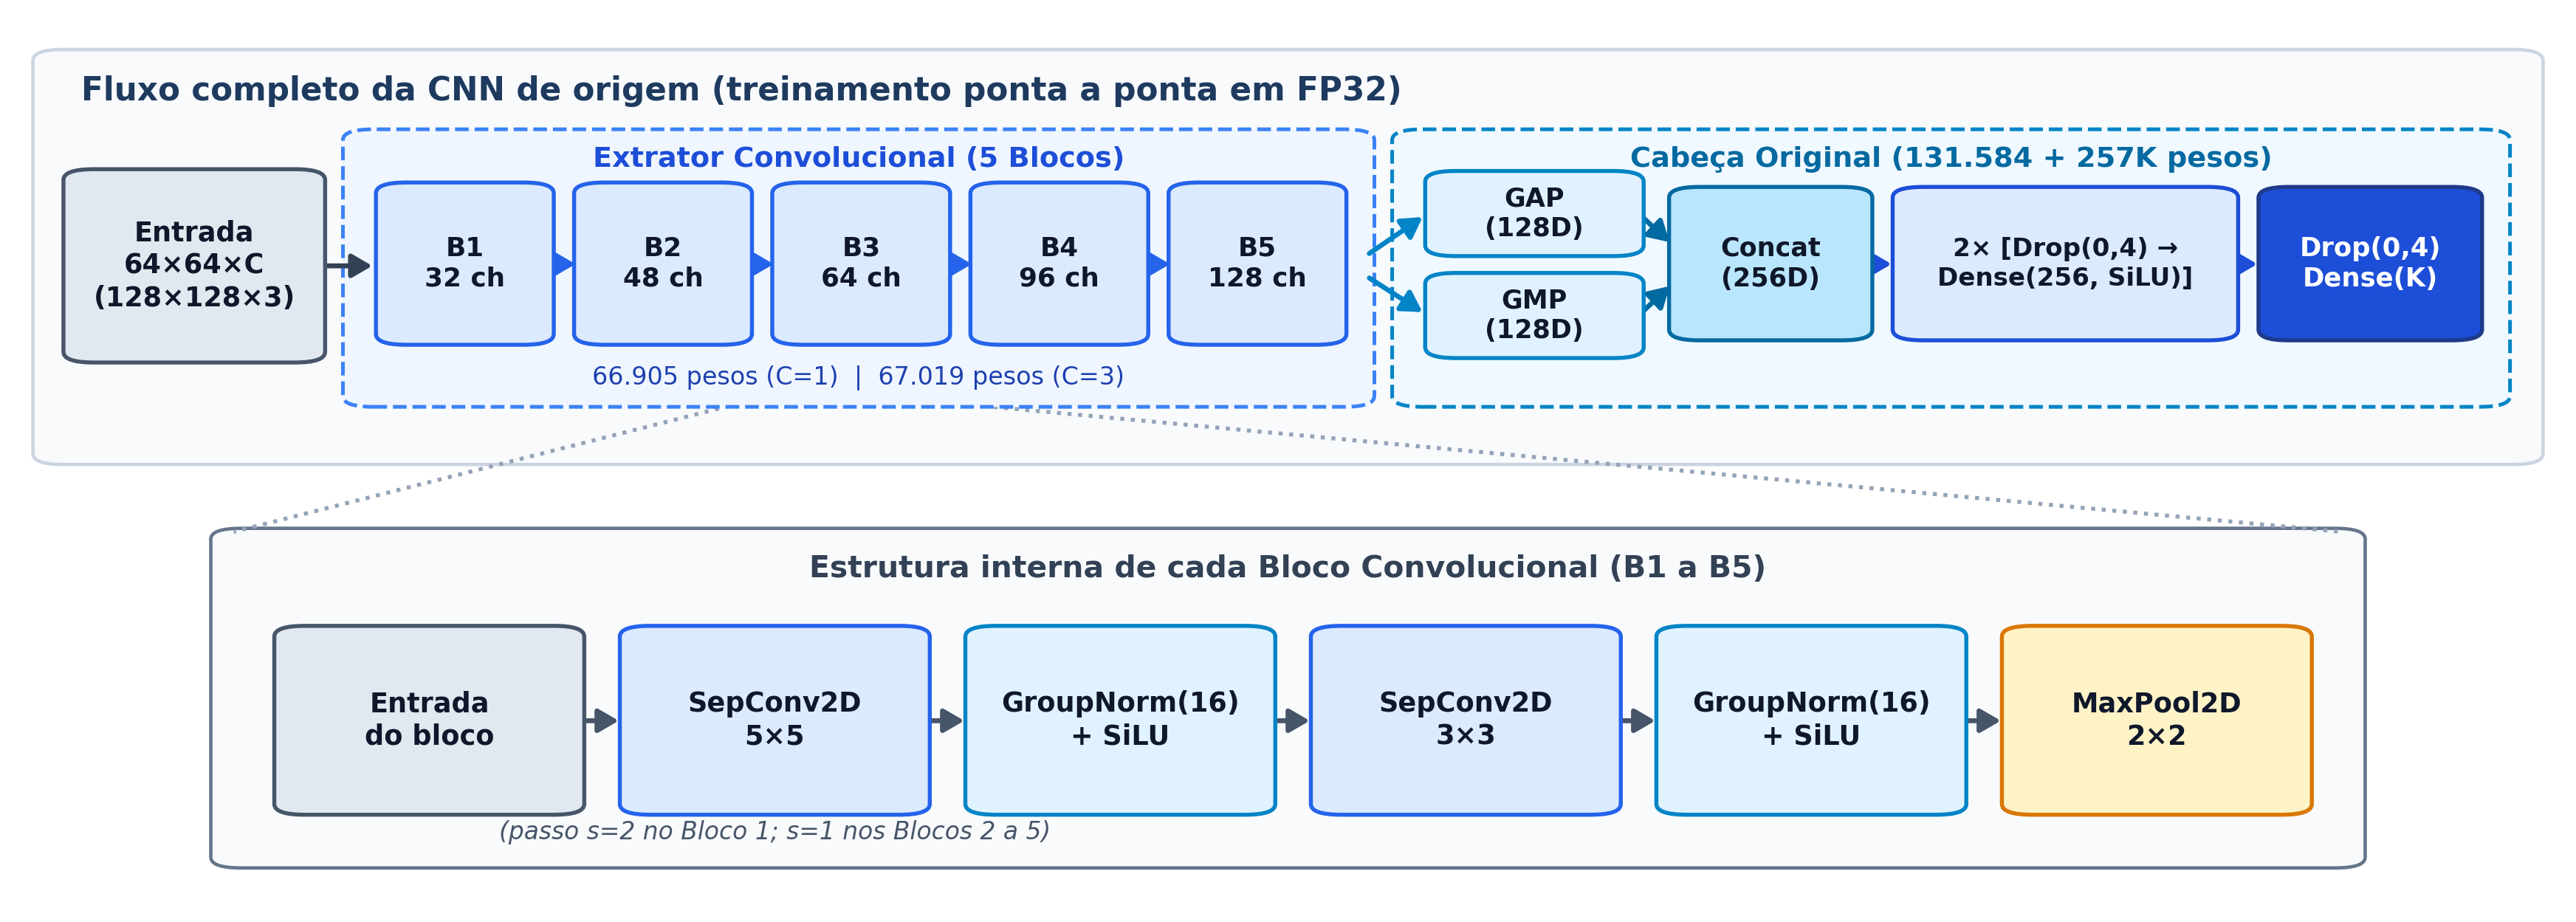
\includegraphics[width=0.98\textwidth,height=0.52\textheight,keepaspectratio]{fig_arq_etapa1_cnn_original.png}
  \vspace{0.12cm}
  \begin{itemize}\footnotesize
    \item Treinada do zero em Linux (FP32, aumento de 50\%, \textit{label smoothing} 0,05); 201.059 pesos ($C=1, K=10$)
    \item Congelada em \texttt{block5\_pool} + GAP para exportar \texttt{features128} determinísticas (\texttt{.npy}) em $\sim 3$ min nas 9 bases
  \end{itemize}
  \fonte{Elaborado pelo autor (2026).}
\end{frame}

% 29b - ANATOMIA INTERNA DE UM BLOCO CNN
\begin{frame}{Anatomia interna de um bloco CNN (Bloco B3)}
  \centering
  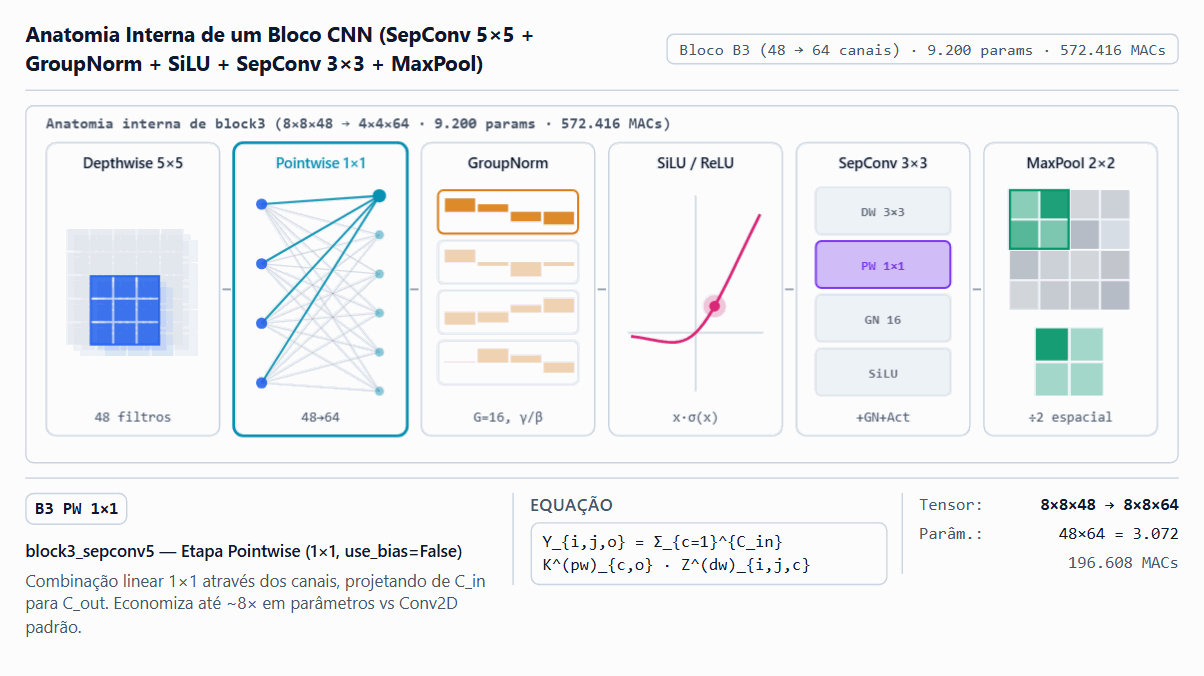
\includegraphics[width=0.98\textwidth,height=0.56\textheight,keepaspectratio]{fig_arq_bloco_cnn_anatomia.png}
  \vspace{0.10cm}
  \begin{itemize}\footnotesize
    \item Sequência por bloco: \texttt{SepConv 5×5 + GroupNorm(16) + SiLU + SepConv 3×3 + MaxPool 2×2}
    \item Exemplo no Bloco B3 ($8\times 8\times 48 \to 4\times 4\times 64$): \textbf{9.200 parâmetros} e 572.416 MACs, com normalização independente de lote
  \end{itemize}
  \fonte{Elaborado pelo autor (2026).}
\end{frame}

% 30a - ETAPA 2A: Dense20 SOBRE IMAGENS
\begin{frame}{Etapa 2A: cabeça \texttt{Dense20} sobre imagens}
  \centering
  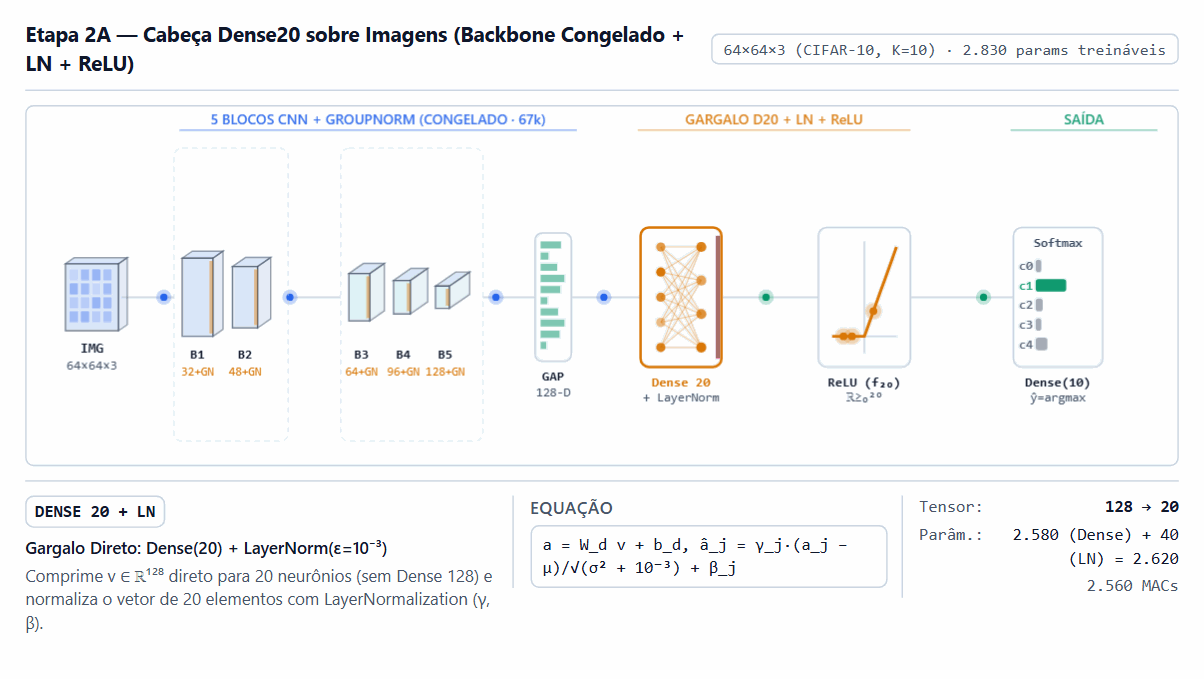
\includegraphics[width=0.98\textwidth,height=0.56\textheight,keepaspectratio]{fig_arq_etapa2a_dense20_imagem.png}
  \vspace{0.10cm}
  \begin{itemize}\footnotesize
    \item Mantém os 5 blocos convolucionais congelados processando imagens com aumento de dados de 50\% em Linux
    \item Gargalo direto \texttt{GAP(128) $\to$ Dense(20) + LayerNorm + ReLU $\to$ Dense(K)} com \textbf{2.830 pesos treináveis} ($K=10$)
  \end{itemize}
  \fonte{Elaborado pelo autor (2026).}
\end{frame}

% 30b - ETAPA 2B: CABEÇA CLÁSSICA VETORIAL
\begin{frame}{Etapa 2B: cabeça clássica vetorial (\texttt{Dense20})}
  \centering
  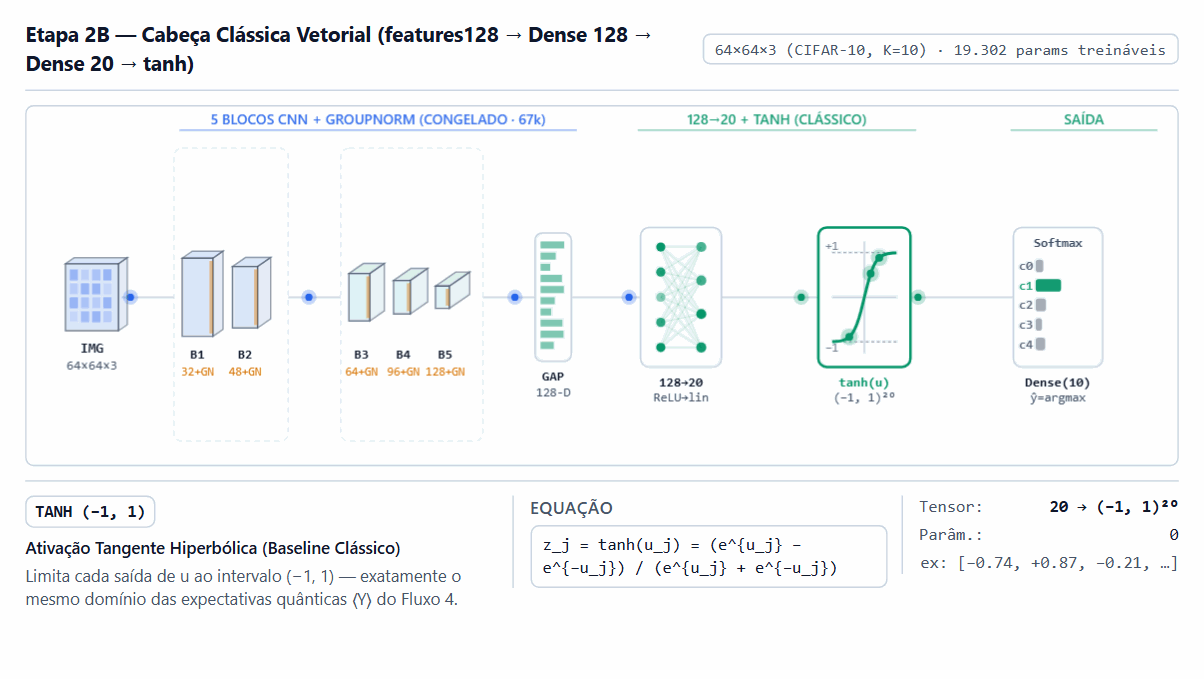
\includegraphics[width=0.98\textwidth,height=0.56\textheight,keepaspectratio]{fig_arq_etapa2b_dense20_vetorial.png}
  \vspace{0.10cm}
  \begin{itemize}\footnotesize
    \item Atua diretamente sobre \texttt{features128} congelados em \texttt{.npy}: \texttt{Dense(128, ReLU) $\to$ Dense(20) $\to$ tanh $\to$ Dense(K)}
    \item Soma \textbf{19.302 pesos treináveis} ($K=10$); constitui o controle clássico 1:1 da camada quântica em Linux e Mac
  \end{itemize}
  \fonte{Elaborado pelo autor (2026).}
\end{frame}

% 31 - ETAPA 3: CABEÇA HÍBRIDA
\begin{frame}{Etapa 3: cabeça híbrida paralela ($4\times 5$ qubits)}
  \centering
  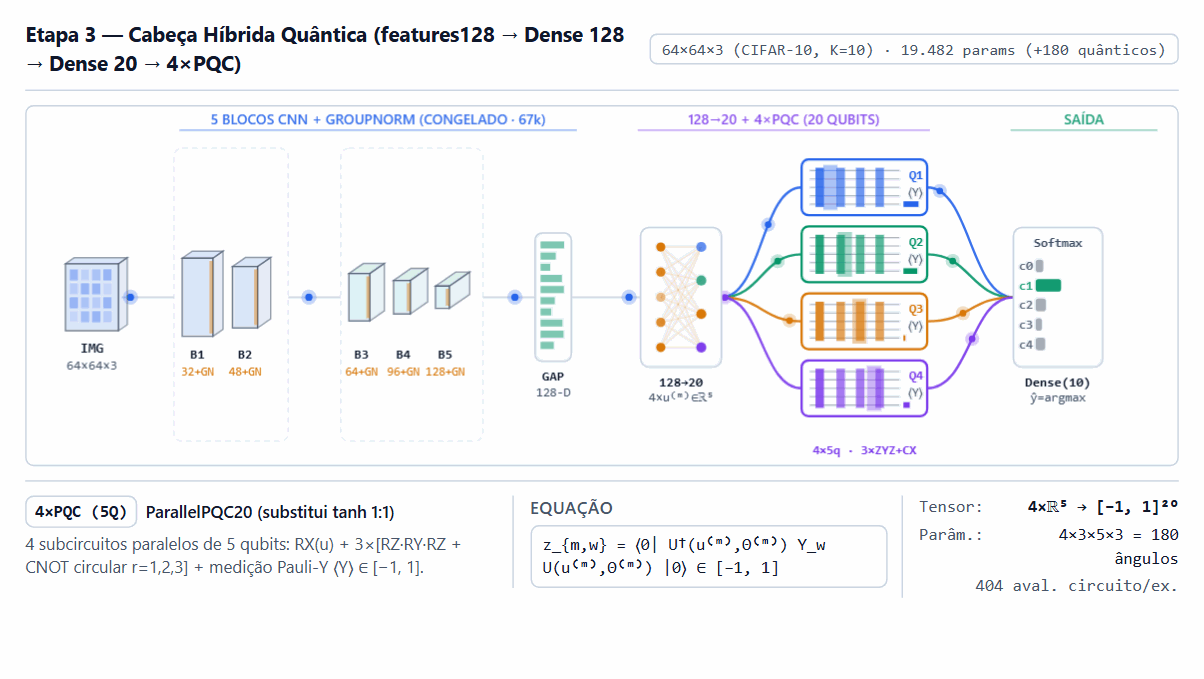
\includegraphics[width=0.98\textwidth,height=0.52\textheight,keepaspectratio]{fig_arq_etapa3_hibrida_4x5.png}
  \vspace{0.12cm}
  \begin{itemize}\footnotesize
    \item Recebe exatamente as mesmas \texttt{features128} e projeção $128\to 20$ da cabeça vetorial clássica
    \item Vetor $u\in\mathbb{R}^{20}$ dividido em 4 ramos disjuntos de 5 qubits sem emaranhamento cruzado (19.482 pesos, $K=10$)
  \end{itemize}
  \fonte{Elaborado pelo autor (2026), com base em Senokosov et al.\ (2024).}
\end{frame}

% 32 - CIRCUITO VARIACIONAL DE 5 QUBITS
\begin{frame}{Circuito variacional de 5 qubits por ramo}
  \centering
  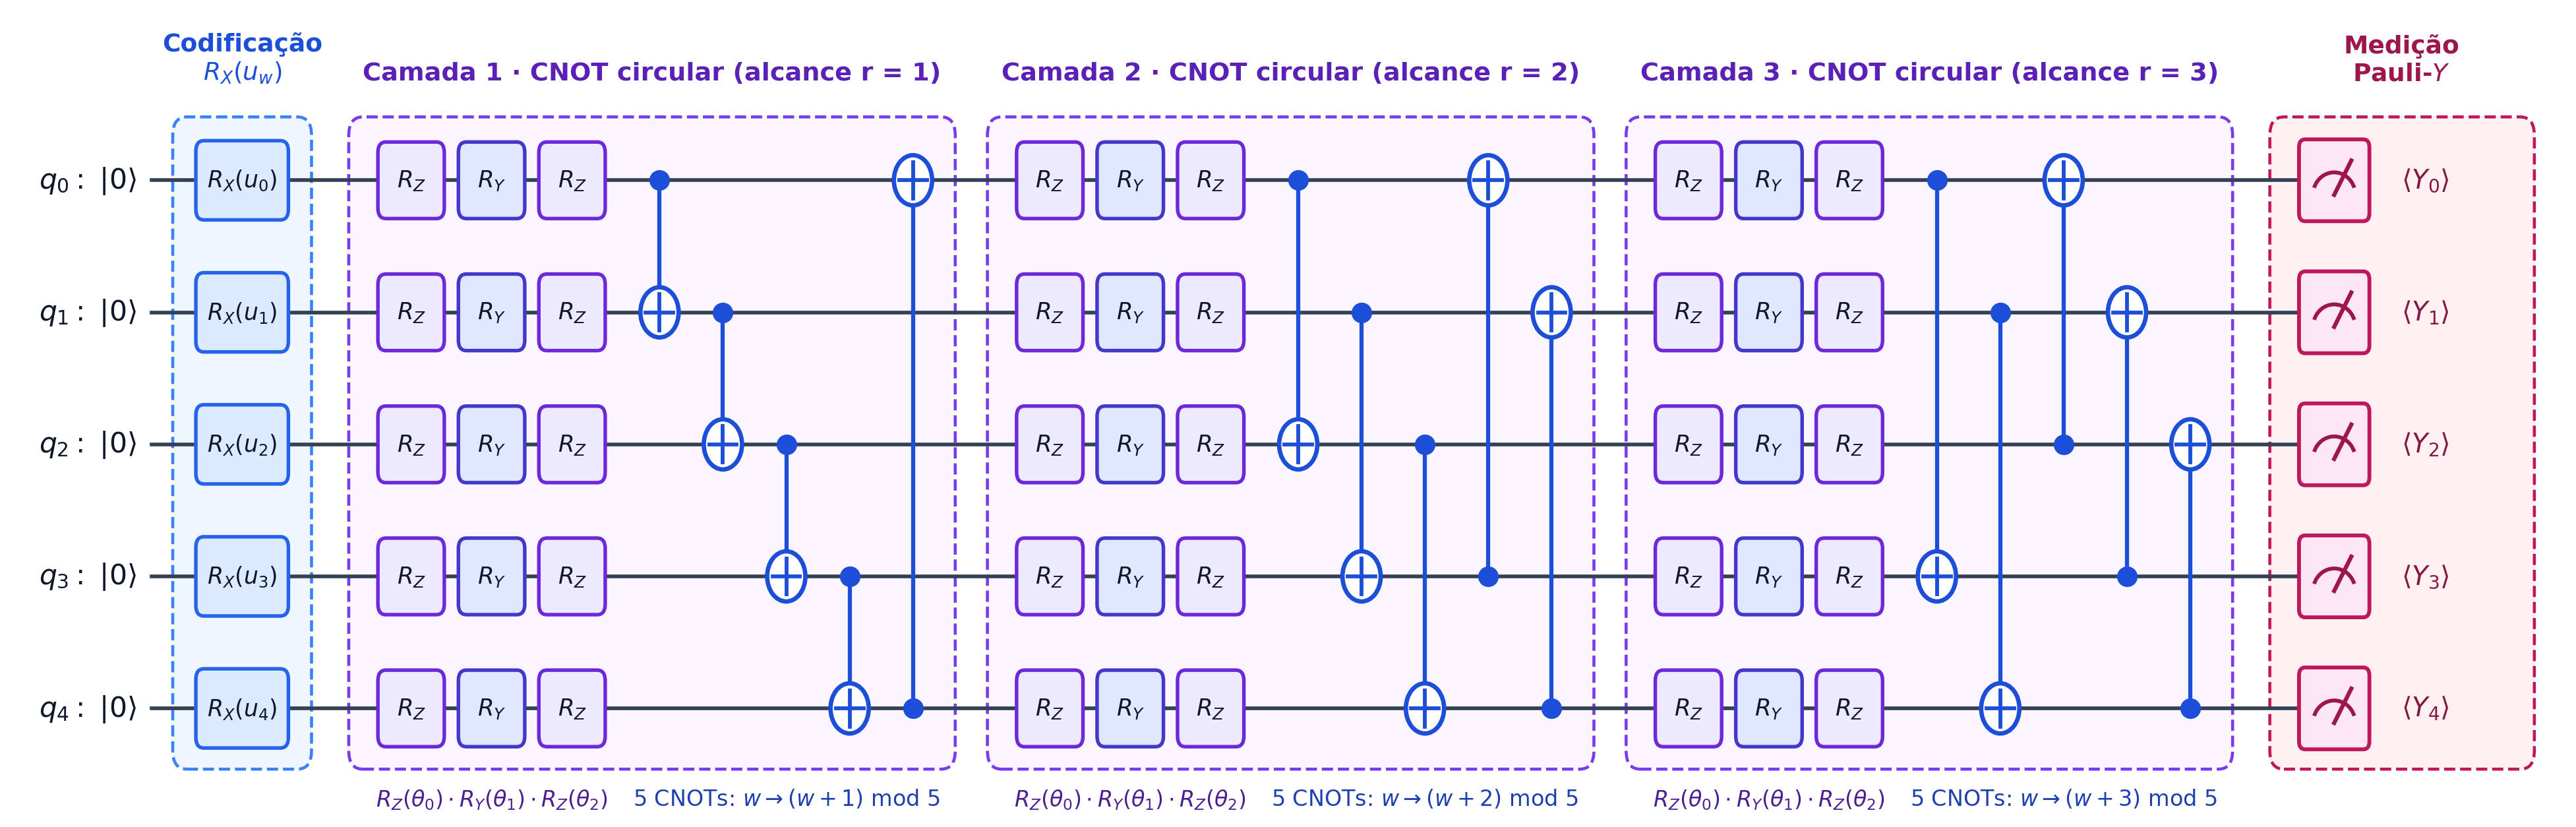
\includegraphics[width=0.98\textwidth,height=0.48\textheight,keepaspectratio]{fig_circuito_quantico_5qubits.png}
  \vspace{0.14cm}
  \begin{itemize}\footnotesize
    \item Codificação angular $R_X$ + 3 camadas $R_Z$--$R_Y$--$R_Z$ com CNOT circular (alcances $r=1,2,3$) + medição Pauli-$Y$
    \item \textbf{Custo do \textit{parameter-shift}:} 45 pesos/ramo (180 quânticos) $\Rightarrow$ 404 avaliações lógicas/amostra no treino e 4 na inferência
  \end{itemize}
  \fonte{Elaborado pelo autor (2026), reproduzindo Senokosov et al.\ (2024).}
\end{frame}

% 33 - COMPARATIVO ESTRUTURAL
\begin{frame}{Comparativo estrutural: o que mudou entre as etapas}
  \centering
  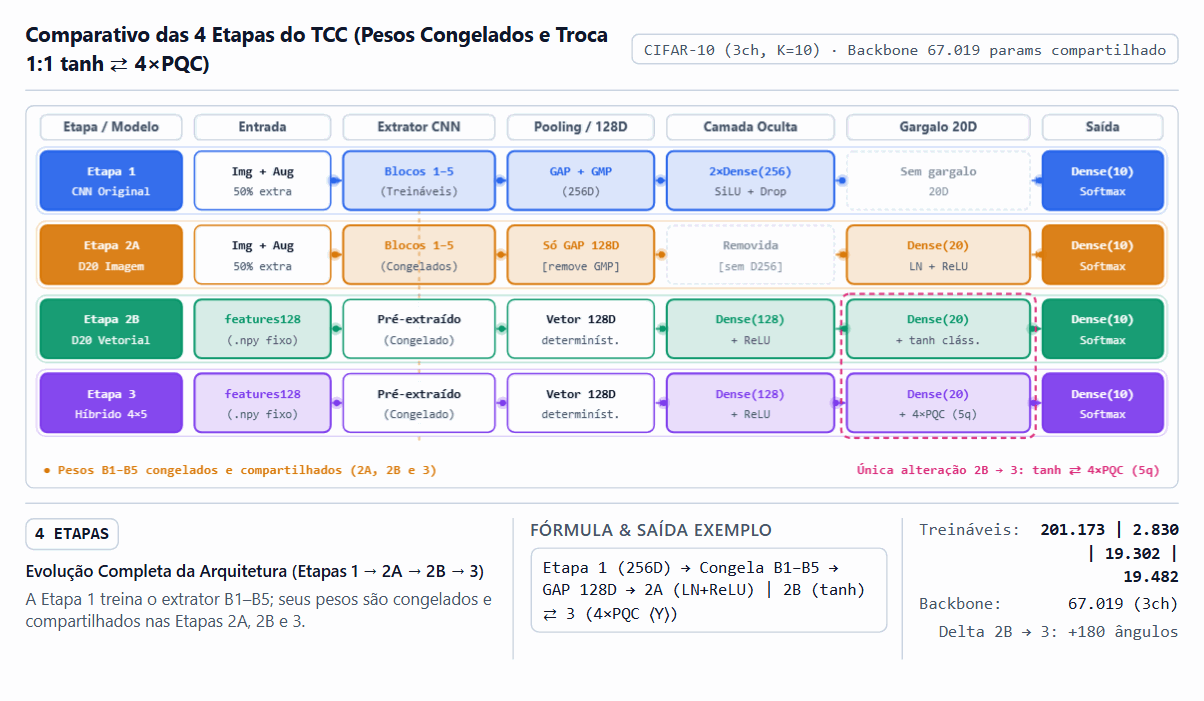
\includegraphics[width=0.98\textwidth,height=0.56\textheight,keepaspectratio]{fig_arq_comparativo_mudancas.png}\par\vspace{0.12cm}
  {\footnotesize\bfseries\color{senacblue}Da Etapa 2B (\texttt{Dense20} vetorial) para a Etapa 3 (Híbrido), altera-se apenas a não linearidade de 20 dimensões: $\tanh \leftrightarrow 4\times 5$ qubits.}
  \fonte{Elaborado pelo autor (2026).}
\end{frame}

% 34 - PROTOCOLO EXPERIMENTAL
\begin{frame}{Protocolo experimental e critérios de avaliação}
  \begin{columns}[T,onlytextwidth]
    \begin{column}{0.48\textwidth}
      \begin{block}{Regime de treinamento (\texttt{seed=42})}
        \begin{itemize}\setlength{\itemsep}{4pt}
          \item 72 checkpoints (9 bases $\times$ 8 configurações), 100 épocas completas
          \item Otimizador Adam ($\eta = 3\times 10^{-4}$, cosseno + aquecimento)
          \item Seleção pelo melhor Macro-F1 de validação; teste final em \texttt{all\_raw}
          \item Imagens: \textit{label smoothing} 0,05; \texttt{features128}: entropia cruzada padrão, lote 128
        \end{itemize}
      \end{block}
    \end{column}
    \begin{column}{0.48\textwidth}
      \begin{block}{Métrica primária}
        Macro-F1 de teste (\%) e $\Delta$ pareado em pontos percentuais (p.p.).
      \end{block}
      \vspace{0.12cm}
      \begin{block}{Critérios de auditoria}
        \begin{itemize}\setlength{\itemsep}{3pt}
          \item Convergência estável acima do acaso ($1/K$)
          \item 1.336 posteriores bayesianas (Jeffreys) e calibração (ECE, NLL, Brier)
          \item 576 Grad-CAM, 73.728 oclusões $8\times 8$, gradientes, ruído/shots e telemetria
        \end{itemize}
      \end{block}
    \end{column}
  \end{columns}
\end{frame}

% 35 - DOIS AMBIENTES COMPUTACIONAIS
\begin{frame}{Dois ambientes computacionais e versões auditadas}
  \centering
  {\footnotesize
  \begin{tabular}{@{}lR{5.2cm}R{5.2cm}@{}}
    \toprule
    \textbf{Componente} & \textbf{Ambiente 1: Win / WSL2} & \textbf{Ambiente 2: iMac M4} \\
    \midrule
    SO / Arq. & Ubuntu 22.04.5 (WSL2) + Win nativo (x86-64) & macOS 15.5 (ARM64, Metal) \\
    CPU & Intel Core i7-14700K (28 lógicos) & Apple Silicon M4 (P/E-cores) \\
    Memória & $\approx 15$ GiB (WSL) + 4 GiB swap & 16 GB de memória unificada \\
    GPU & NVIDIA RTX A2000 12GB (CUDA 13.2) & GPU Apple M4 10 núcleos (AGX) \\
    Deep Learning & TensorFlow 2.21.0; Keras 3.12.4 & TF 2.18.1; Metal 1.2; PyTorch 2.8.0 \\
    Simulação / Tel. & PennyLane \& Qiskit Aer (Win); psutil, NVML & PennyLane 0.44.1; Qiskit 2.3.0; Aer 0.17.2; \texttt{macmon} \\
    \bottomrule
  \end{tabular}}
  \fonte{Elaborado pelo autor (2026).}
\end{frame}

% 36 - TABELA MACRO-F1
\begin{frame}{Macro-F1 de teste (\%) nas nove bases}
  \centering
  {\footnotesize
  \begin{tabular}{@{}lrrrrr@{}}
    \toprule
    \textbf{Base} & \textbf{CNN orig.} & \textbf{Dense20} & \textbf{Híbrido} & \textbf{$\Delta$ Híb$-$CNN} & \textbf{$\Delta$ Híb$-$D20} \\
    \midrule
    MNIST & 98,984 & 99,225 & 99,305 & +0,321 & +0,080 \\
    Fashion-MNIST & 91,915 & 92,050 & 91,894 & $-0{,}021$ & $-0{,}156$ \\
    KMNIST & 98,649 & 98,648 & 98,648 & $-0{,}001$ & 0,000 \\
    EMNIST Balanced & 87,719 & 88,642 & 88,474 & +0,755 & $-0{,}168$ \\
    CIFAR-10 & 73,117 & 73,389 & 73,320 & +0,203 & $-0{,}069$ \\
    CIFAR-100 Coarse & 47,458 & 47,559 & 47,117 & $-0{,}341$ & $-0{,}442$ \\
    SVHN & 92,088 & 92,567 & 92,634 & +0,546 & +0,067 \\
    GTSRB* & 99,365 & 99,633 & 99,590 & +0,225 & $-0{,}043$ \\
    FER2013 & 48,158 & 47,899 & 48,519 & +0,361 & +0,620 \\
    \bottomrule
  \end{tabular}}
  \vspace{0.15cm}
  {\footnotesize\color{textmuted}*GTSRB: 67,9\% do teste em \textit{tracks} do treino. Dense20 e Híbrido: Mac/PennyLane (desvio PL vs.\ QK $< 0{,}05$ p.p.).}
  \fonte{Elaborado pelo autor (2026).}
\end{frame}

% 37 - GRÁFICO DOS DELTAS
\begin{frame}{Quanto o híbrido difere? ($\Delta$ em pontos percentuais)}
  \centering
  \begin{tikzpicture}
    \begin{axis}[
      ybar, bar width=6.5pt, width=0.96\textwidth, height=0.58\textheight,
      ymin=-0.55, ymax=0.90, ylabel={$\Delta$ Macro-F1 (p.p.)},
      symbolic x coords={MNIST,F-MN,KMN,EMNIST,CIF10,C100C,SVHN,GTSRB,FER13},
      xtick=data, tick label style={font=\footnotesize}, label style={font=\footnotesize},
      ymajorgrids=true, grid style={dashed,gray!40},
      legend style={at={(0.5,1.03)},anchor=south,legend columns=-1,draw=none,font=\footnotesize}
    ]
      \addplot[fill=senacblue,draw=senacblue] coordinates {
        (MNIST,0.321)(F-MN,-0.021)(KMN,-0.001)(EMNIST,0.755)(CIF10,0.203)(C100C,-0.341)(SVHN,0.546)(GTSRB,0.225)(FER13,0.361)
      };
      \addplot[fill=senacorange,draw=senacorange] coordinates {
        (MNIST,0.080)(F-MN,-0.156)(KMN,0.000)(EMNIST,-0.168)(CIF10,-0.069)(C100C,-0.442)(SVHN,0.067)(GTSRB,-0.043)(FER13,0.620)
      };
      \legend{Híbrido $-$ CNN original, Híbrido $-$ Dense20}
    \end{axis}
  \end{tikzpicture}
  \vspace{0.05cm}
  {\footnotesize\bfseries\color{senacblue}Frente à CNN: média +0,23 p.p.\ \;|\; Frente ao Dense20: média $-0{,}01$ p.p.\ (16/36 positivos e 20/36 negativos nos pares).}
  \fonte{Elaborado pelo autor (2026).}
\end{frame}

% 38 - PAPEL DO CONTROLE Dense20
\begin{frame}{O papel do controle \texttt{Dense20} e eficiência paramétrica}
  \begin{columns}[T,onlytextwidth]
    \begin{column}{0.48\textwidth}
      \begin{alertblock}{Sem o controle, haveria ``ganhos''}
        Híbrido $-$ CNN: EMNIST +0,755 p.p., SVHN +0,546 p.p., FER2013 +0,361 p.p., MNIST +0,321 p.p., GTSRB +0,225 p.p.
      \end{alertblock}
    \end{column}
    \begin{column}{0.48\textwidth}
      \begin{block}{Com o controle, o ganho some}
        \texttt{Dense20} já explica a maior parte: EMNIST 88,642 (vs.\ 88,474), CIFAR-10 73,389 (vs.\ 73,320), GTSRB 99,633 (vs.\ 99,590), KMNIST 98,648.
      \end{block}
    \end{column}
  \end{columns}
  \vspace{0.25cm}
  \begin{itemize}\footnotesize\setlength{\itemsep}{6pt}
    \item \textbf{Gargalo clássico:} o ganho frente à CNN vem da regularização em 20 dimensões, não de vantagem quântica
    \item \textbf{Parâmetros ($C=1, K=10$):} CNN 201,1k $\to$ inferência completa usa 69,7k (D20 img), 86,2k (Vet) e 86,4k (Híb) --- redução real de 57\%--65\%, mantendo os 66,9k pesos do extrator
  \end{itemize}
\end{frame}

% 39 - COMPLEXIDADE DO DOMÍNIO
\begin{frame}{Complexidade do domínio governa o desempenho}
  \centering
  \begin{tikzpicture}
    \begin{axis}[
      xbar, bar width=7pt, width=0.88\textwidth, height=0.52\textheight,
      xmin=0, xmax=112, xlabel={Macro-F1 do híbrido (\%)},
      symbolic y coords={CIFAR-100C,FER2013,CIFAR-10,EMNIST,F-MNIST,SVHN,KMNIST,MNIST},
      ytick=data, tick label style={font=\footnotesize}, label style={font=\footnotesize},
      nodes near coords, every node near coord/.append style={font=\footnotesize},
      xmajorgrids=true, grid style={dashed,gray!40}
    ]
      \addplot[fill=senacblue,draw=senacblue] coordinates {
        (47.1,CIFAR-100C)(48.5,FER2013)(73.3,CIFAR-10)(88.5,EMNIST)(91.9,F-MNIST)(92.6,SVHN)(98.6,KMNIST)(99.3,MNIST)
      };
    \end{axis}
  \end{tikzpicture}
  \vspace{0.05cm}
  \begin{itemize}\footnotesize
    \item \textbf{Amplitude estreita por base:} 0,085 p.p.\ (KMNIST) a 1,124 p.p.\ (EMNIST) --- \texttt{features128} governam o teto preditivo
    \item \textbf{Domínios difíceis:} CIFAR-100 Coarse (5 classes finas/superclasse) e FER2013 (desgosto com 82 amostras no teste)
  \end{itemize}
  \fonte{Elaborado pelo autor (2026).}
\end{frame}

% 40 - GTSRB: INTERPRETAÇÃO CAUTELOSA
\begin{frame}{GTSRB: números altos, interpretação cautelosa}
  \begin{columns}[T,onlytextwidth]
    \begin{column}{0.38\textwidth}
      \begin{block}{Macro-F1 observado}
        \centering\vspace{0.35cm}
        {\large\bfseries\color{senacblue}99,365\% \; CNN}\\[10pt]
        {\large\bfseries\color{senacblue}99,633\% \; Dense20}\\[10pt]
        {\large\bfseries\color{senacblue}99,590\% \; Híbrido}
        \vspace{0.35cm}
      \end{block}
    \end{column}
    \begin{column}{0.58\textwidth}
      \begin{alertblock}{Por que exigir cautela?}
        3.990 de 5.876 imagens de teste (67,9\%) pertencem a \textit{tracks} físicos já presentes no treino (quadros correlacionados da mesma placa).
      \end{alertblock}
      \vspace{0.15cm}
      \begin{block}{Incerteza bayesiana (classe 0, $N=31$)}
        Mesmo com F1 observado de 100\%, o IC 95\% de Jeffreys vai de 94,15\% a 99,96\% ($\mathbb{P}(F_1>99\%)=46{,}74\%$).
      \end{block}
    \end{column}
  \end{columns}
\end{frame}

% 41 - EXPLICABILIDADE ESPACIAL
\begin{frame}{Explicabilidade espacial: Grad-CAM vs.\ oclusão $8\times 8$}
  \begin{columns}[T,onlytextwidth]
    \begin{column}{0.48\textwidth}
      \begin{block}{Escala da auditoria espacial}
        \begin{itemize}\setlength{\itemsep}{2pt}
          \item \textbf{72 imagens curadas:} 8 por base (4 consensos e 4 divergências, sem duplicatas ou \textit{tracks})
          \item \textbf{576 mapas Grad-CAM:} validados em \texttt{block4\_activation2} ($10^{-4}$) e testes de sanidade
          \item \textbf{73.728 oclusões $8\times 8$:} borramento gaussiano e preenchimento pela média
        \end{itemize}
      \end{block}
    \end{column}
    \begin{column}{0.48\textwidth}
      \begin{alertblock}{Achado central: Spearman $\rho = 0{,}002$}
        \begin{itemize}\setlength{\itemsep}{2pt}
          \item \textcolor{badred}{\textbf{1.152 pares auditados:}} mediana global $\rho = 0{,}002$ ($-0{,}002$ borramento; $+0{,}008$ média)
          \item Grad-CAM em baixa resolução ($4\times 4$/$8\times 8$) não equivale à sensibilidade causal da entrada
          \item Painéis $8\times 8$ revelam divergências de fronteira entre CNN, \texttt{Dense20} e $4\times 5$ qubits
        \end{itemize}
      \end{alertblock}
    \end{column}
  \end{columns}
  \fonte{Elaborado pelo autor (2026), com base em Selvaraju et al.\ (2020), Zeiler e Fergus (2014) e Adebayo et al.\ (2018).}
\end{frame}

% 42 - PAINÉIS CAUSAIS RGB
\begin{frame}{Painéis causais de oclusão: domínios RGB}
  \begin{columns}[T,onlytextwidth]
    \begin{column}{0.48\textwidth}
      \centering
      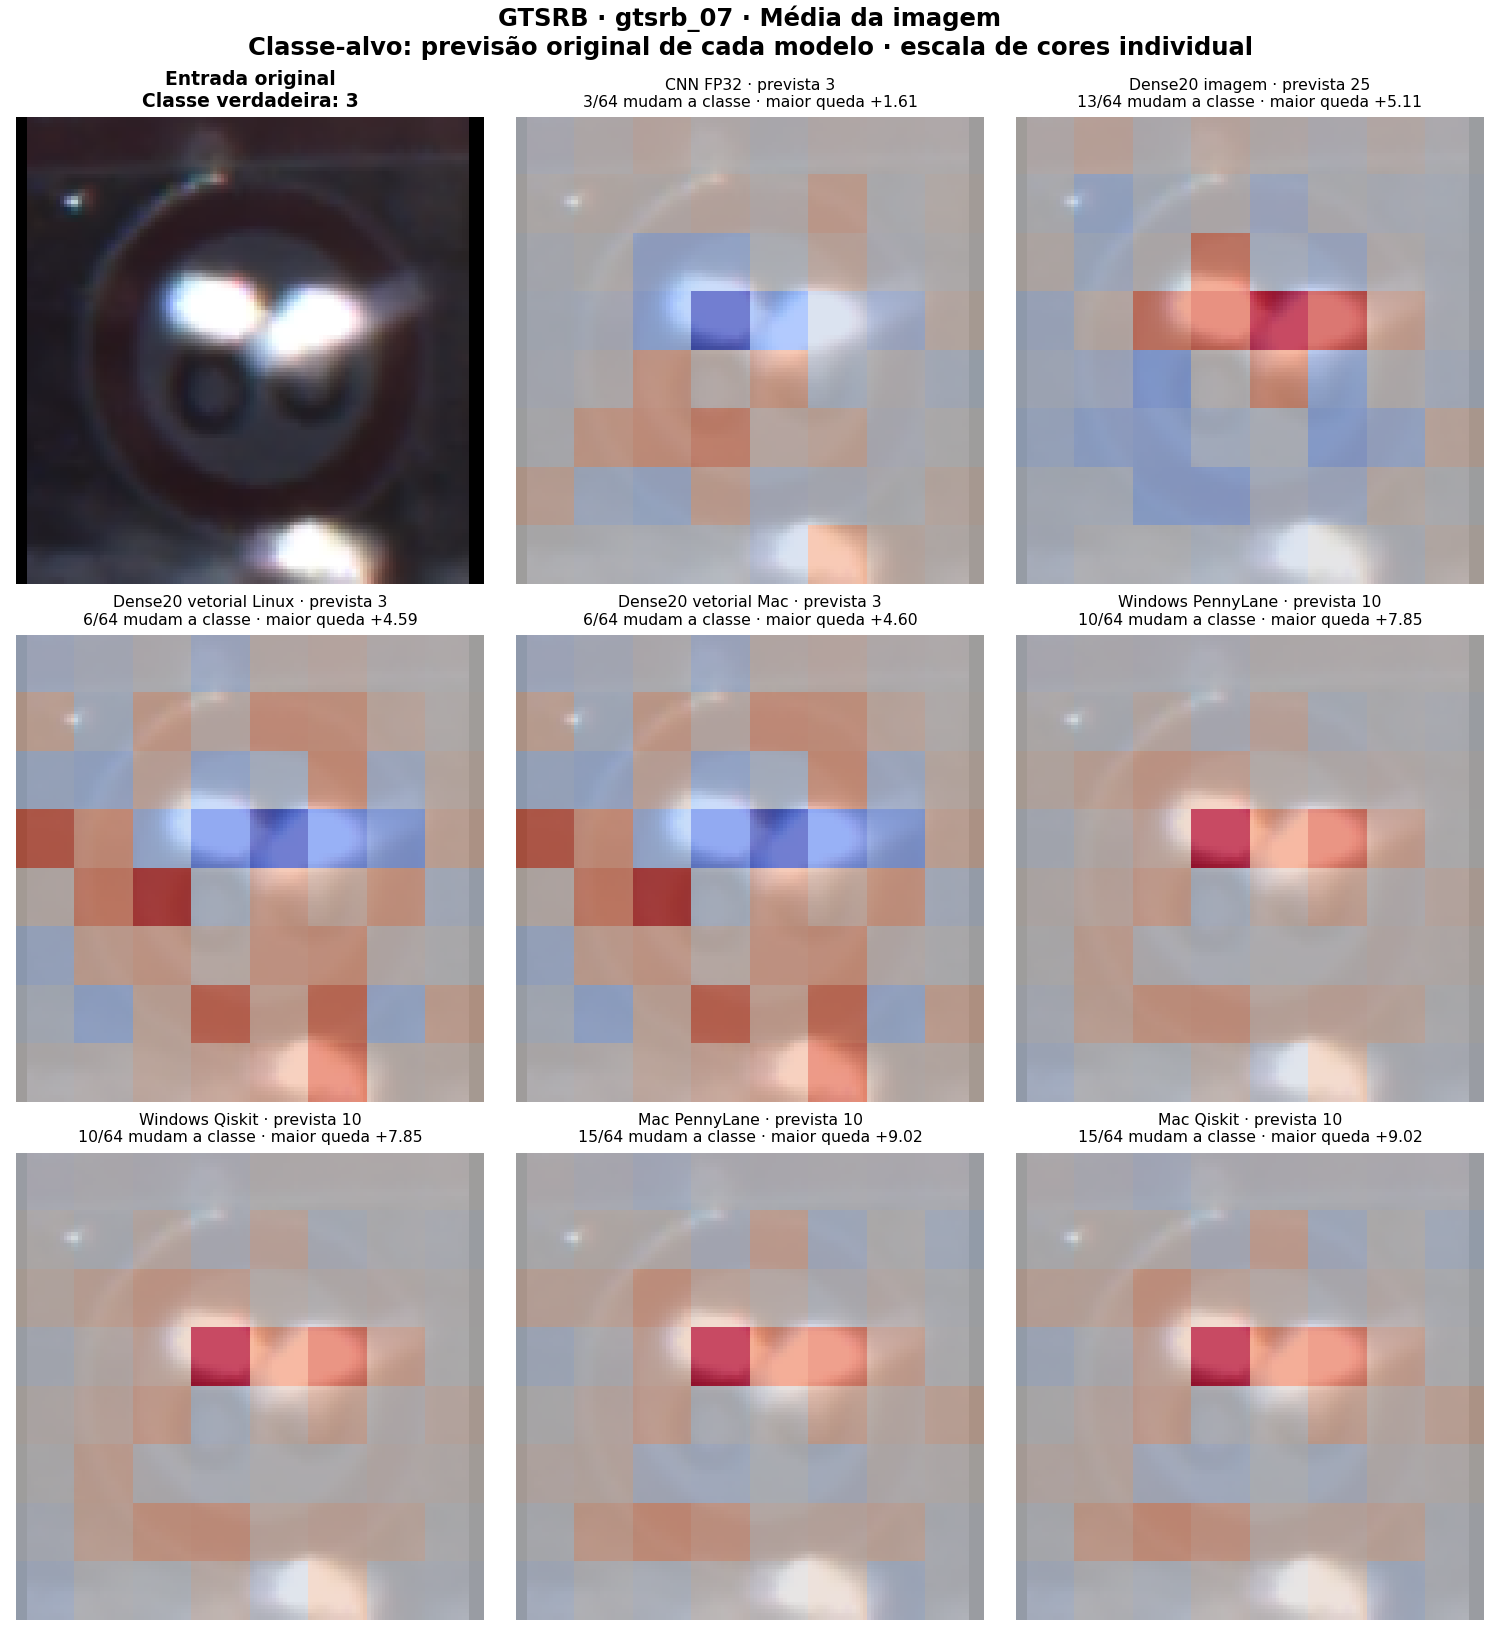
\includegraphics[width=\textwidth,height=0.52\textheight,keepaspectratio]{painel_oclusao_gtsrb_07_media.png}\\[4pt]
      {\footnotesize \texttt{gtsrb\_07} (cl.\ 3, média): CNN/Vet acertam (3--6/64); D20 prevê cl.\ 25; Híbridos cl.\ 10 (10--15/64, até $+9{,}02$).}
    \end{column}
    \begin{column}{0.48\textwidth}
      \centering
      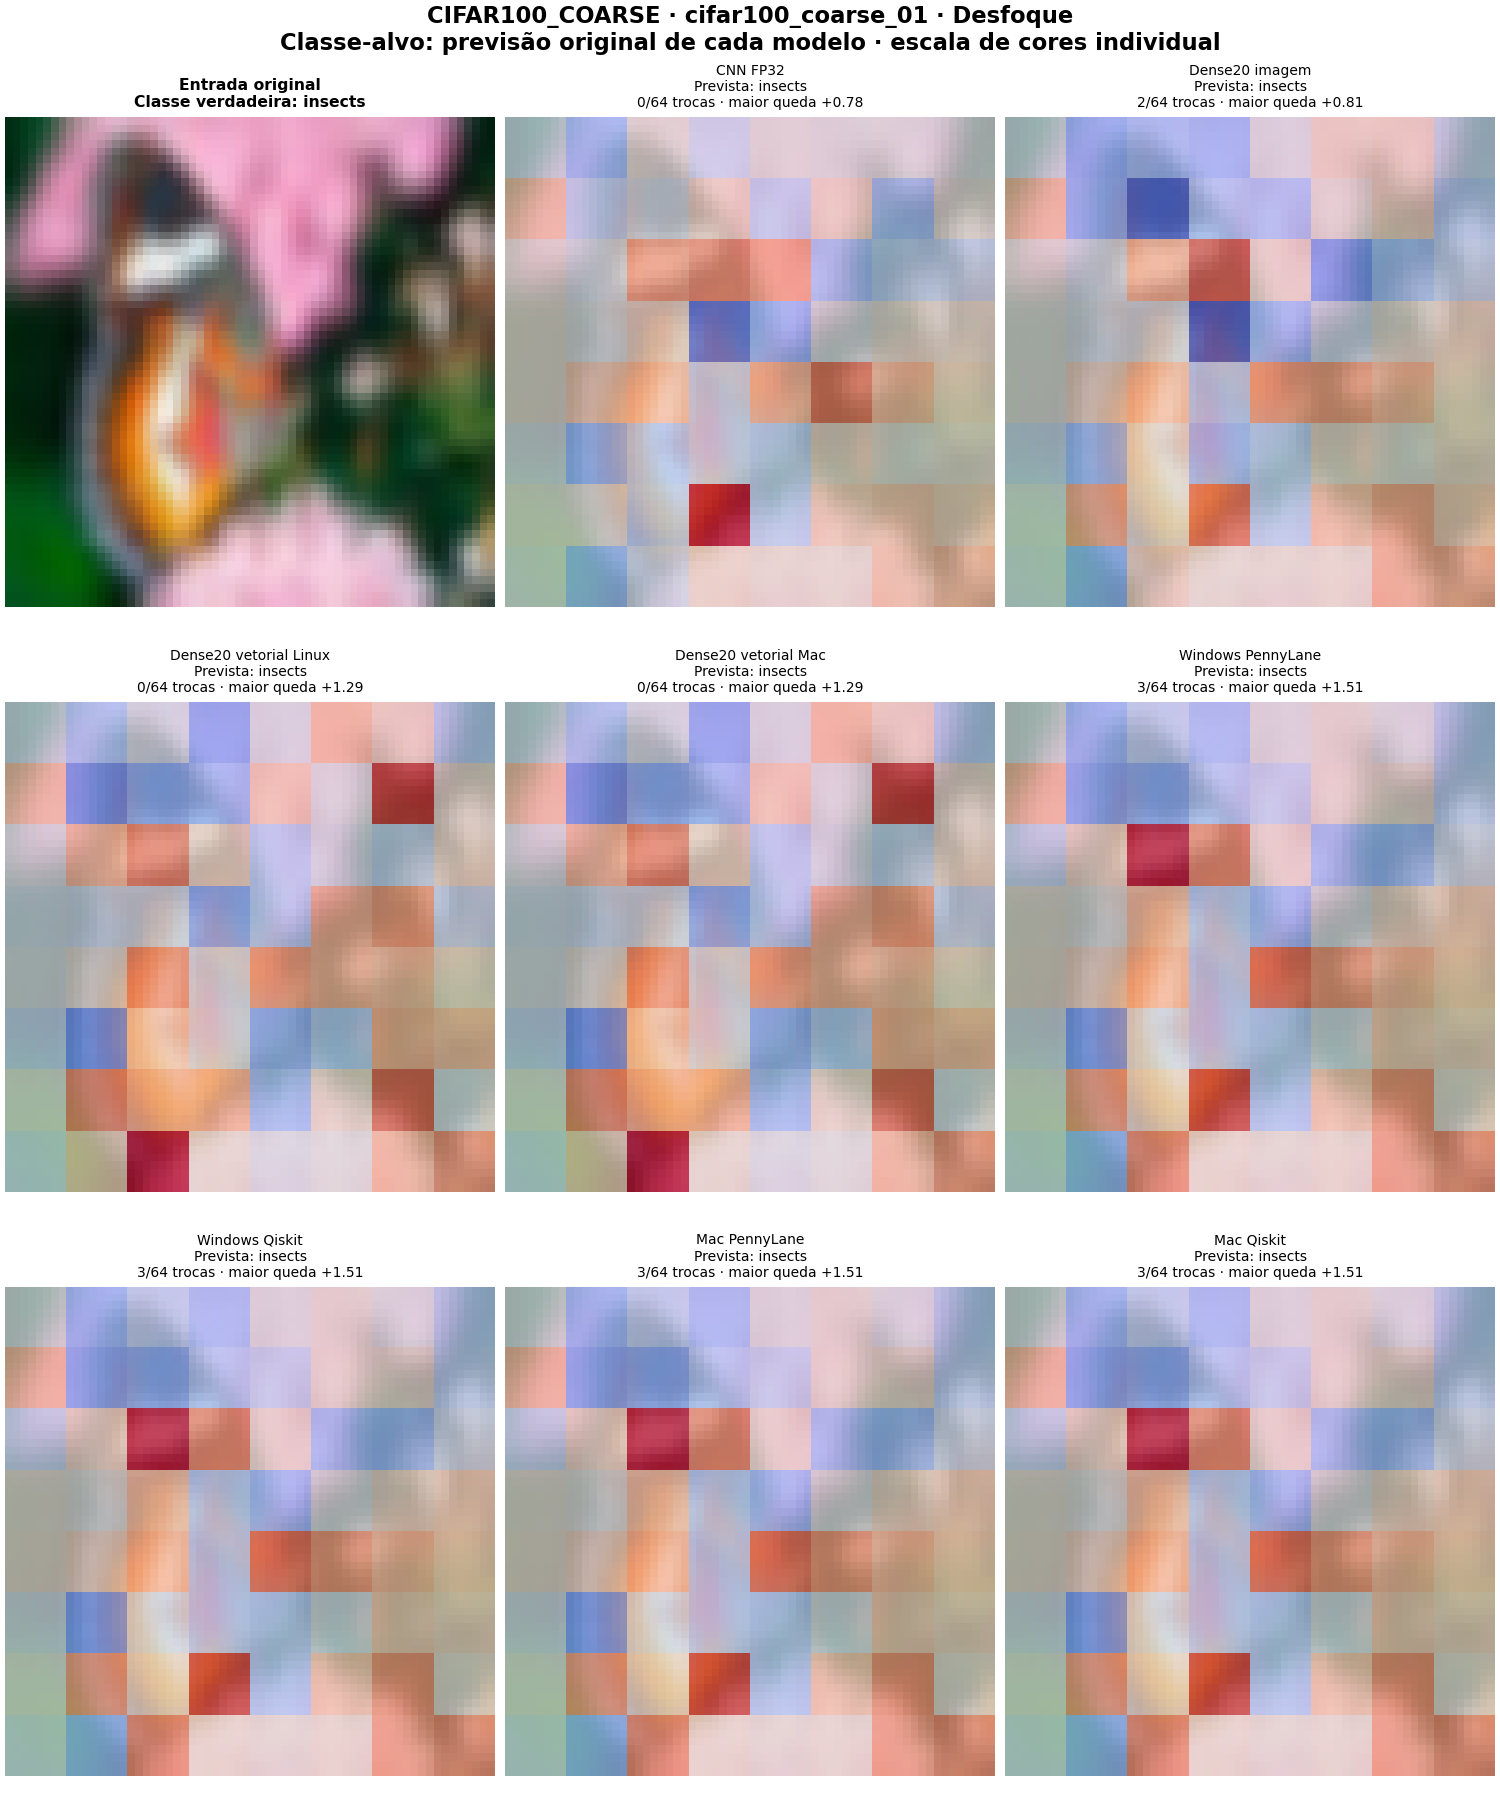
\includegraphics[width=\textwidth,height=0.52\textheight,keepaspectratio]{painel_oclusao_cifar100_coarse_01_desfoque.png}\\[4pt]
      {\footnotesize \texttt{cifar100\_01} (\textit{insects}, desfoque): 8 acertam; CNN/Vet 0/64; D20 2/64; Híbridos 3/64 p/ \textit{flowers} ($+1{,}51$).}
    \end{column}
  \end{columns}
  \fonte{Elaborado pelo autor (2026).}
\end{frame}

% 43 - PAINÉIS CAUSAIS MONOCROMÁTICOS
\begin{frame}{Painéis causais de oclusão: monocromáticos}
  \begin{columns}[T,onlytextwidth]
    \begin{column}{0.48\textwidth}
      \centering
      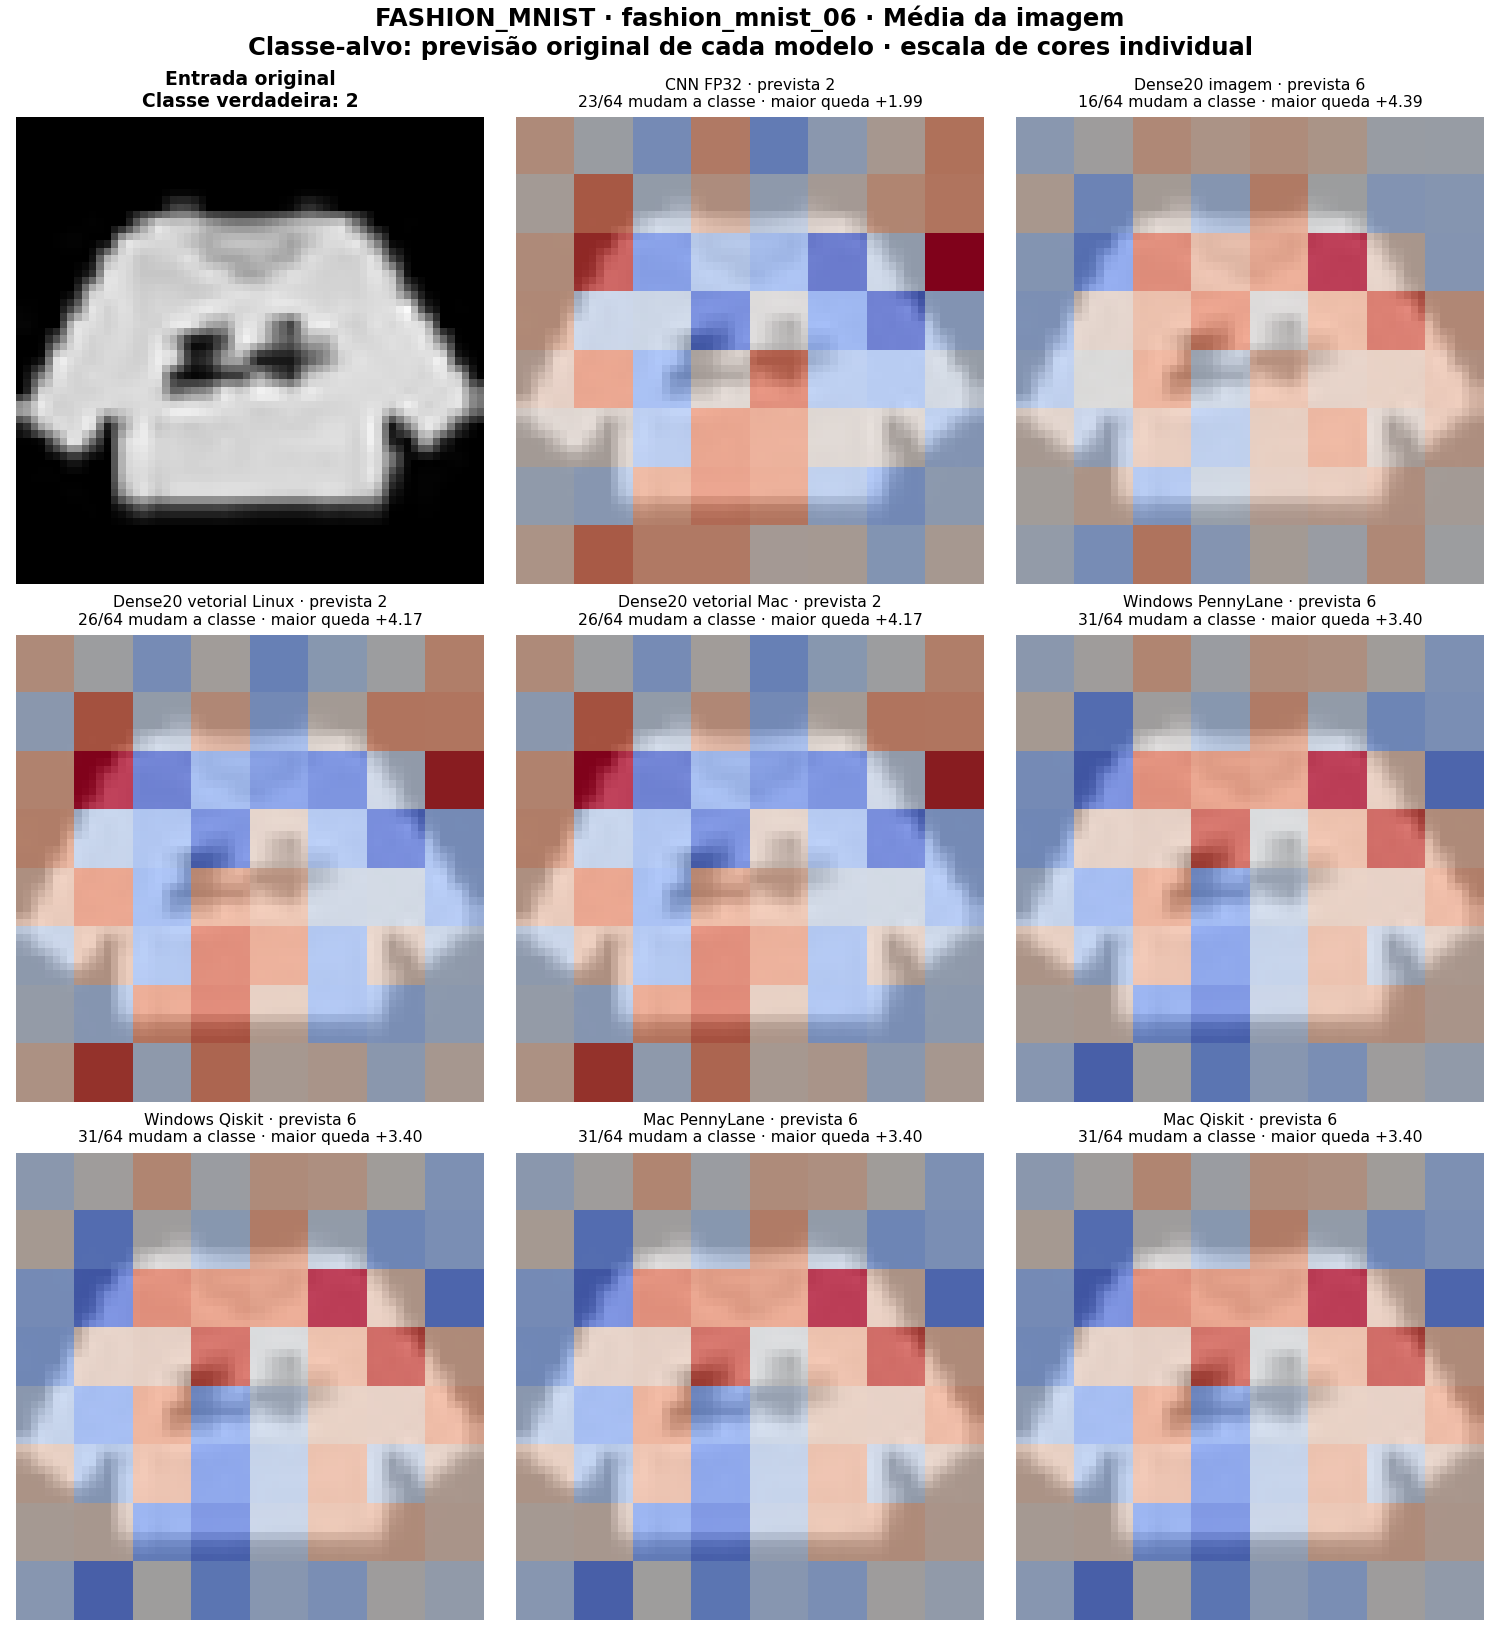
\includegraphics[width=\textwidth,height=0.52\textheight,keepaspectratio]{painel_oclusao_fashion_mnist_06_media.png}\\[4pt]
      {\footnotesize \texttt{fashion\_06} (pulôver, média): CNN/Vet acertam cl.\ 2 (23--26/64); D20 e Híbridos partem da cl.\ 6 (16 e 31/64).}
    \end{column}
    \begin{column}{0.48\textwidth}
      \centering
      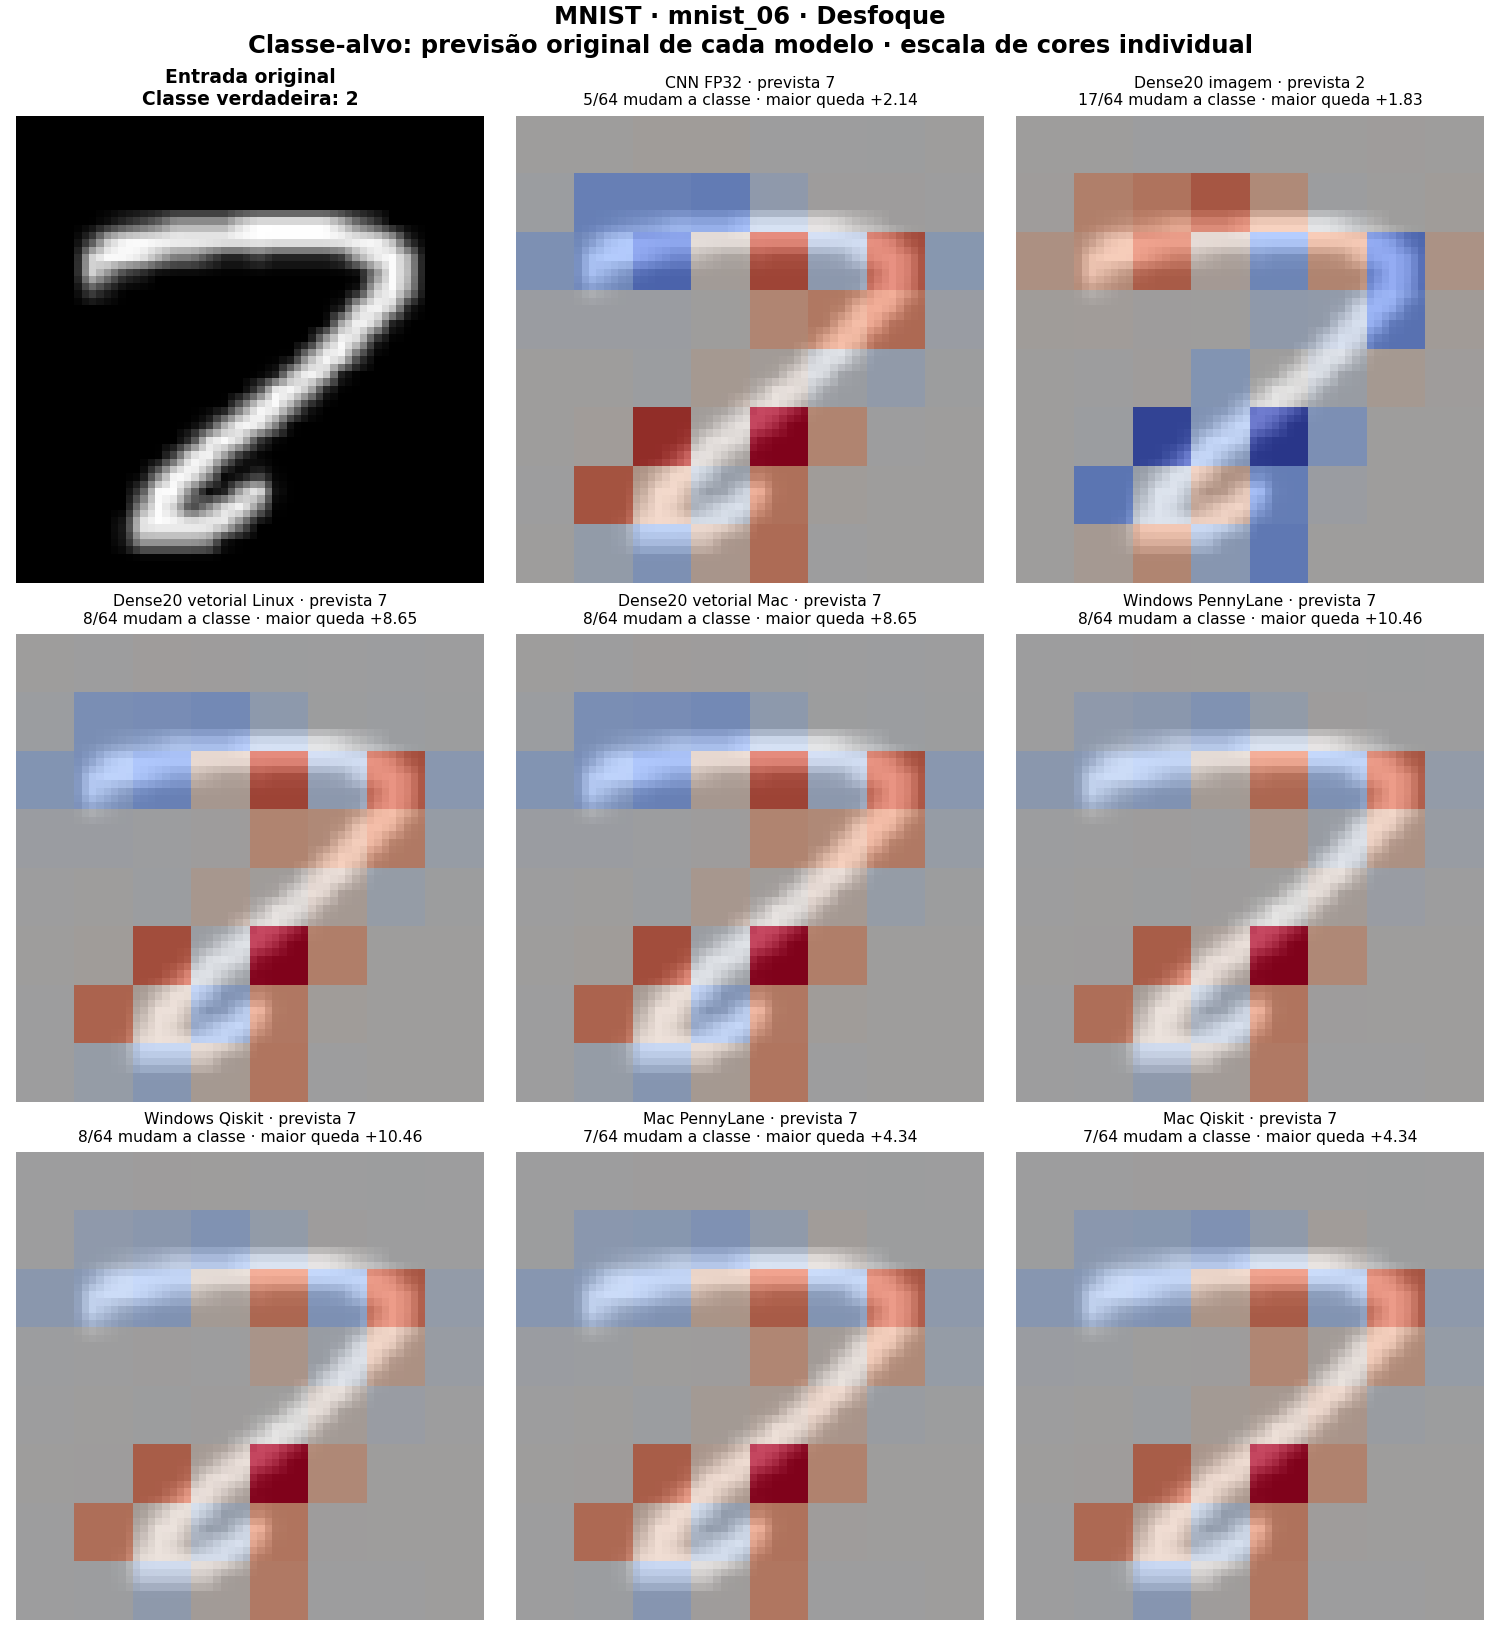
\includegraphics[width=\textwidth,height=0.52\textheight,keepaspectratio]{painel_oclusao_mnist_06_desfoque.png}\\[4pt]
      {\footnotesize \texttt{mnist\_06} (dígito ``2'', desfoque): só D20 img.\ acerta (17/64); CNN, Vet e Híbridos preveem ``7'' (até $+10{,}46$).}
    \end{column}
  \end{columns}
  \fonte{Elaborado pelo autor (2026).}
\end{frame}

% 44 - CUSTO COMPUTACIONAL POR ETAPA (SEÇÃO 4.8 ATUALIZADA)
\begin{frame}{Custo computacional por etapa (100 épocas, lote 128)}
  \begin{columns}[T,onlytextwidth]
    \begin{column}{0.63\textwidth}
      \centering
      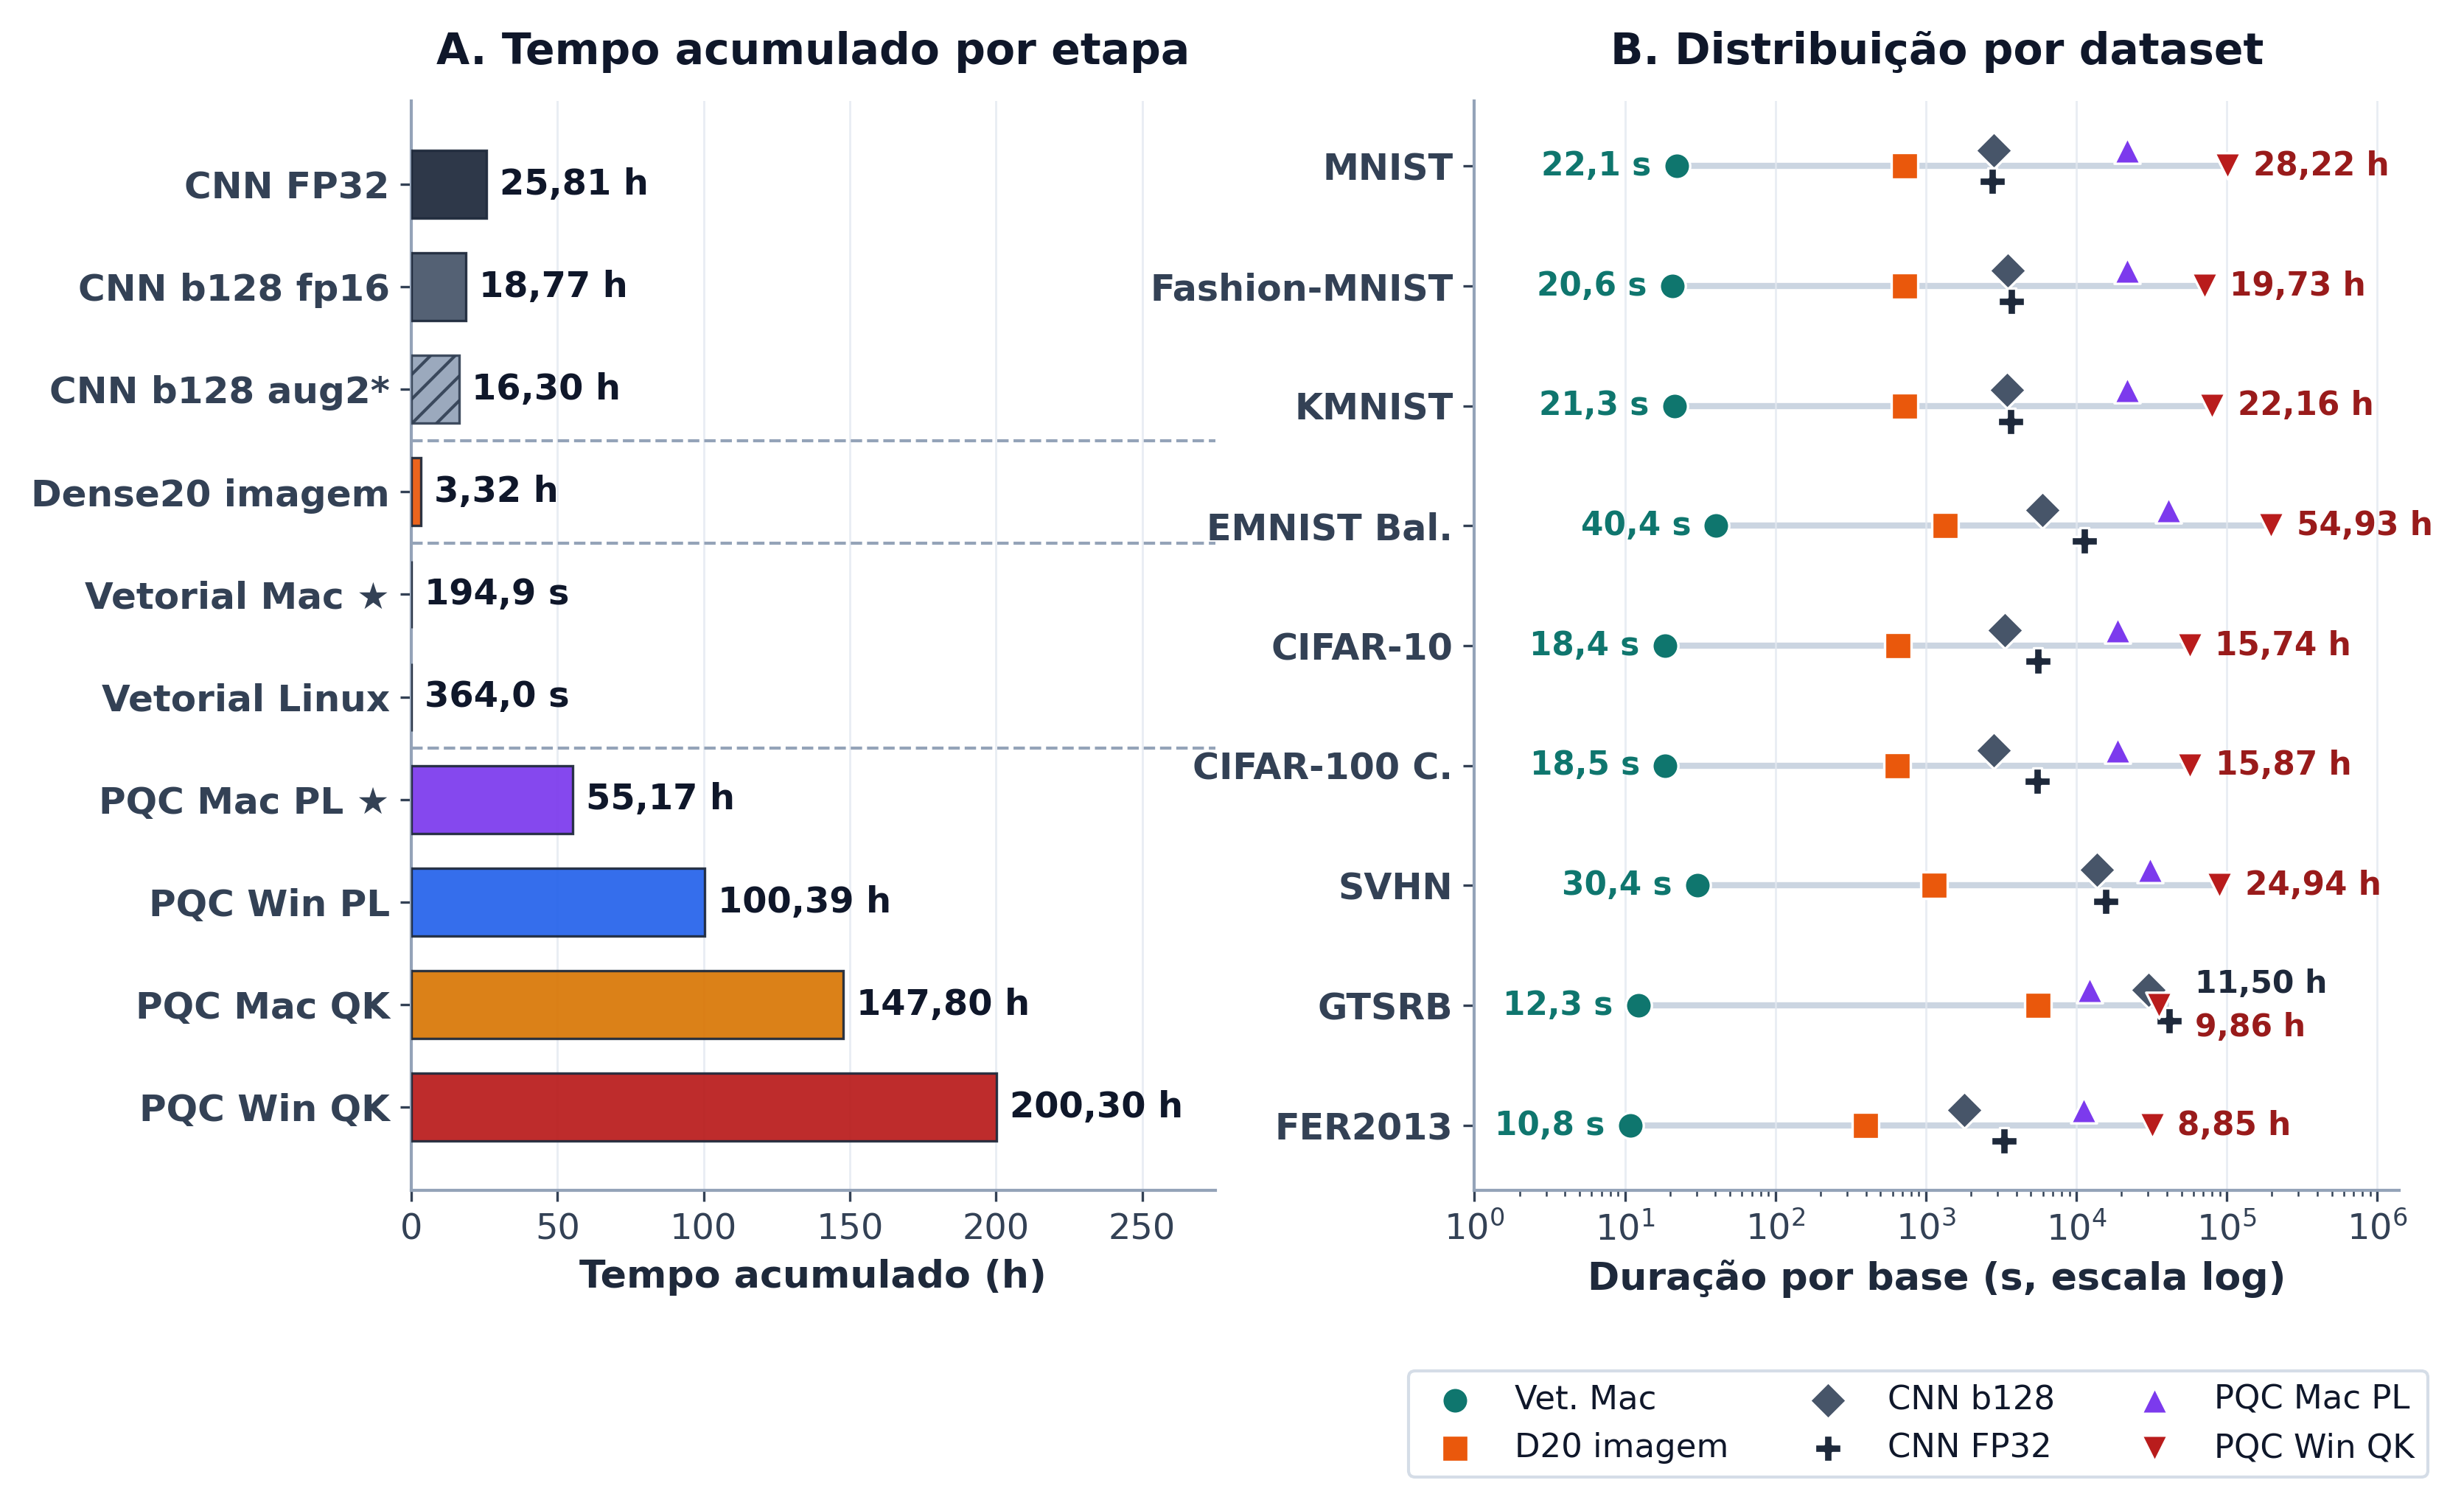
\includegraphics[width=\textwidth,height=0.70\textheight,keepaspectratio]{fig_48_tempos_etapas_consolidado.png}
    \end{column}
    \begin{column}{0.35\textwidth}
      \begin{block}{Gargalo da simulação}
        \begin{itemize}\setlength{\itemsep}{4pt}
          \item \textcolor{badred}{\textbf{36 híbridos:}} 503,66 h (21 dias) vs.\ 18 vetoriais: 558,88 s (9,3 min) --- 778$\times$ a 2.854$\times$
          \item \textcolor{okgreen}{\textbf{Mais rápido:}} \texttt{Dense20} vet.\ Mac (194,86 s; 1.019$\times$ vs.\ Mac PL)
          \item \textbf{Melhor híbrido:} PQC Mac PL (55,17 h) vs.\ Win QK (200,30 h)
          \item CNN FP32: 25,81 h | b128: 18,77 h | D20 img: 3,32 h
        \end{itemize}
      \end{block}
    \end{column}
  \end{columns}
  \fonte{Elaborado pelo autor (2026).}
\end{frame}

% 45 - ACELERAÇÃO ENTRE AMBIENTES E SIMULADORES
\begin{frame}{Aceleração entre ambientes e simuladores}
  \begin{columns}[T,onlytextwidth]
    \begin{column}{0.63\textwidth}
      \centering
      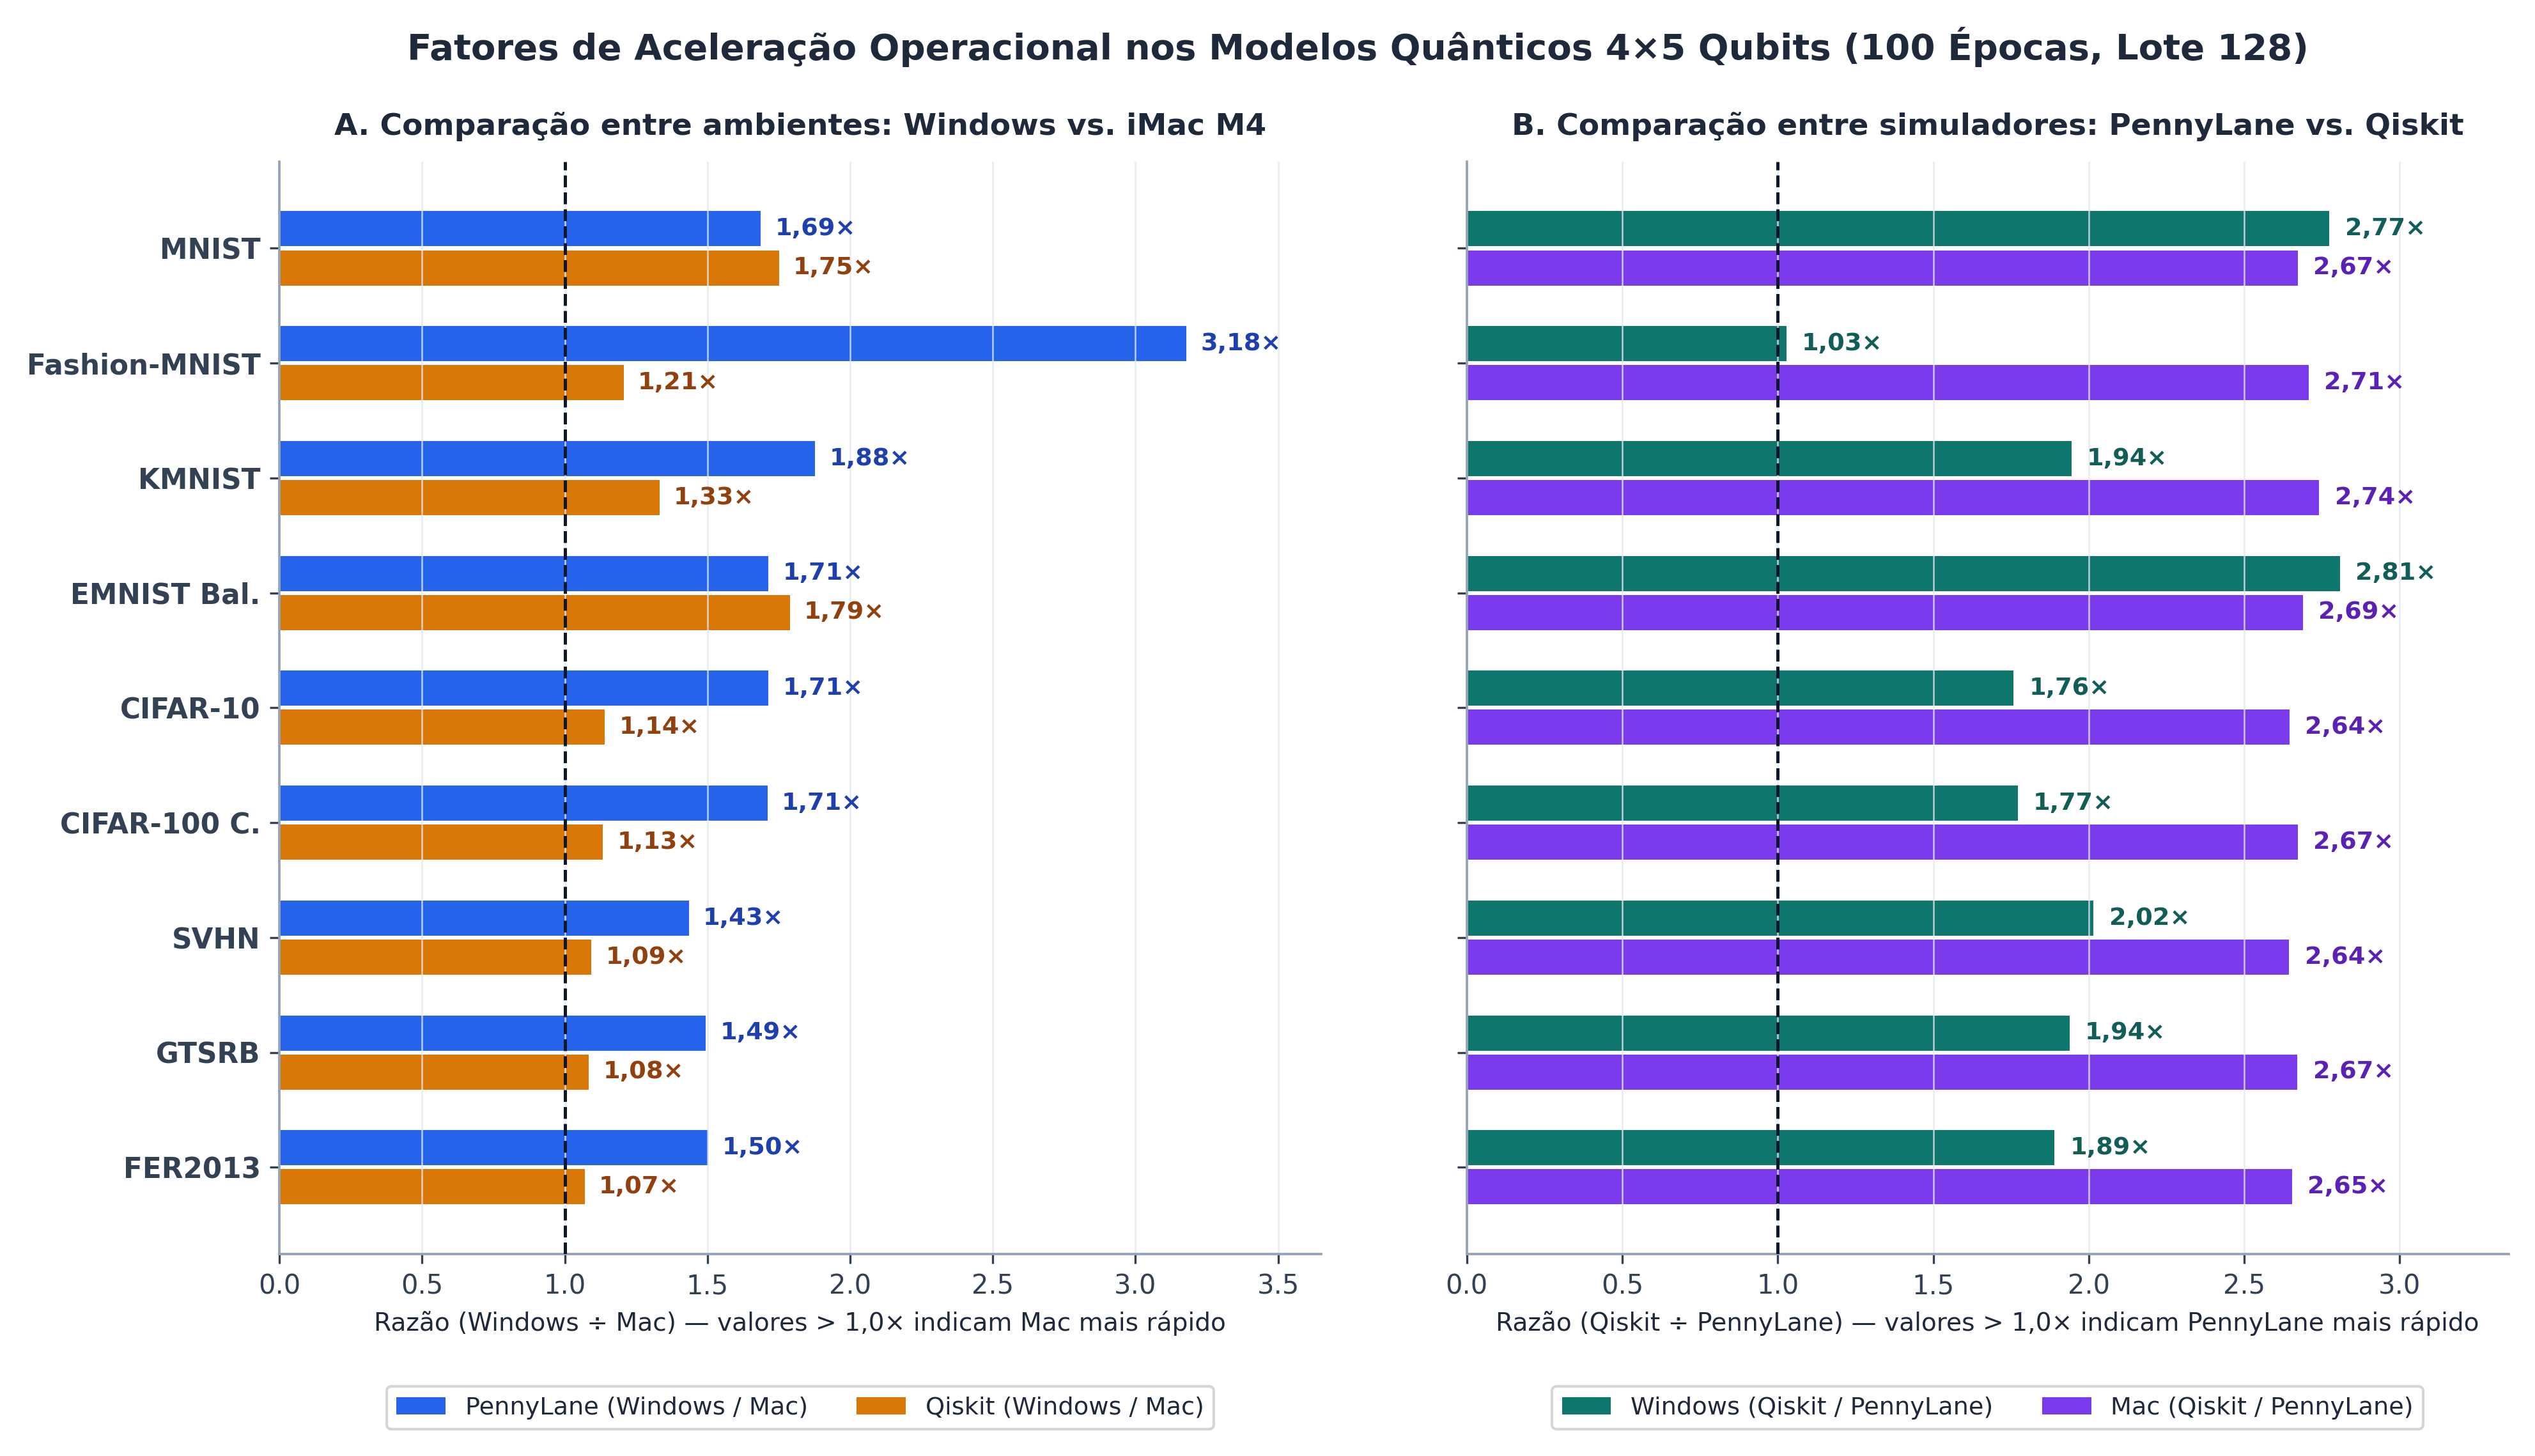
\includegraphics[width=\textwidth,height=0.70\textheight,keepaspectratio]{fig_fatores_aceleracao_ambientes_simuladores.png}
    \end{column}
    \begin{column}{0.35\textwidth}
      \begin{block}{Razões exatas (18/18 pares)}
        \begin{itemize}\setlength{\itemsep}{5pt}
          \item \textcolor{okgreen}{\textbf{iMac M4 vs.\ Windows:}} 1,82$\times$ no PennyLane e 1,36$\times$ no Qiskit (1,87$\times$ vs.\ Linux no vetorial)
          \item \textcolor{okgreen}{\textbf{PennyLane vs.\ Qiskit:}} 2,68$\times$ no Mac e 2,00$\times$ no Windows
          \item \textbf{PQC Mac PennyLane:} 3,63$\times$ mais rápido que Win Qiskit com mesmo Macro-F1 (82,17\%; $\Delta < 0{,}05$ p.p.)
        \end{itemize}
      \end{block}
    \end{column}
  \end{columns}
  \fonte{Elaborado pelo autor (2026).}
\end{frame}

% 46 - TELEMETRIA DE HARDWARE E I/O (100 ÉPOCAS)
\begin{frame}{Telemetria de hardware e I/O (campanha 100 épocas)}
  \begin{columns}[T,onlytextwidth]
    \begin{column}{0.63\textwidth}
      \centering
      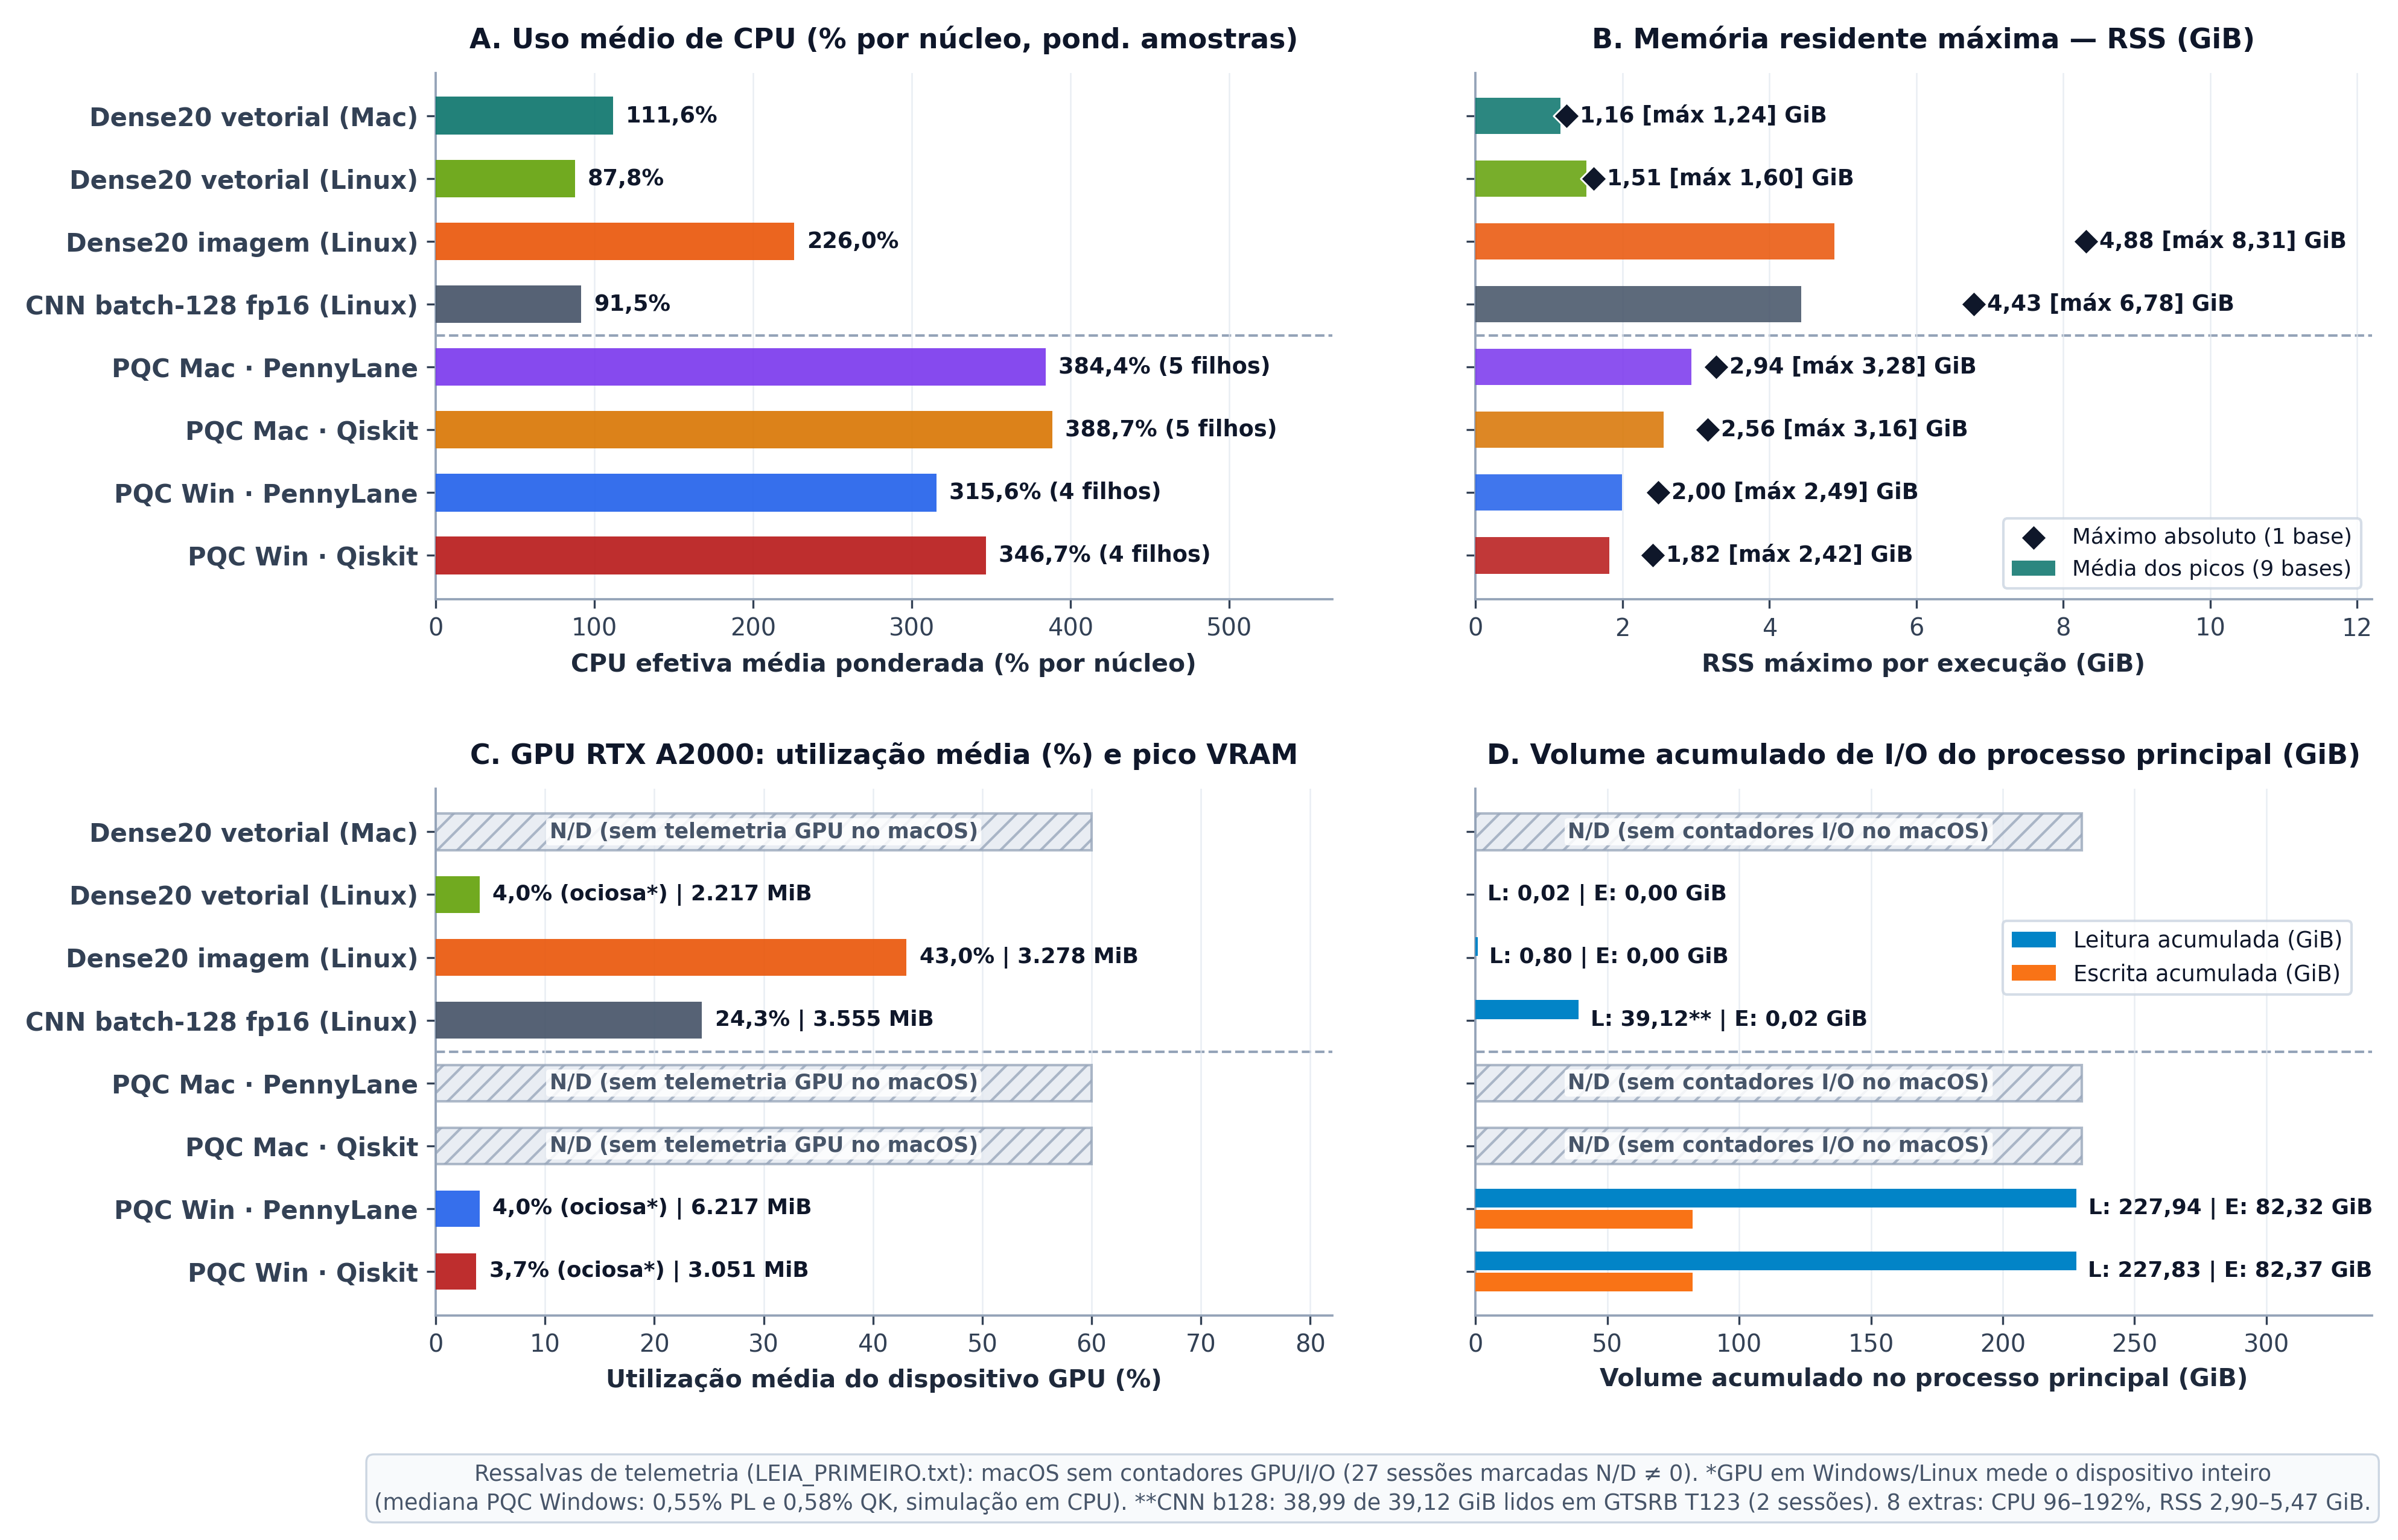
\includegraphics[width=\textwidth,height=0.70\textheight,keepaspectratio]{fig_48_telemetria_hardware_io.png}
    \end{column}
    \begin{column}{0.35\textwidth}
      \begin{block}{Assinaturas de hardware}
        \begin{itemize}\setlength{\itemsep}{5pt}
          \item \textbf{Mac (M4):} 384--389\% CPU ($\approx 4$ núcleos), 2,56--2,94 GiB RSS; GPU AGX 0,00--0,51\%* e I/O proj.\ 3,2--8,5* GiB
          \item \textcolor{badred}{\textbf{Windows (PQC):}} 316--347\% CPU, GPU ociosa (3,7--4,0\%) e 456 GiB leitura / 165 GiB escrita
          \item \textcolor{okgreen}{\textbf{Linux/WSL2:}} GPU RTX A2000 ativa (24--43\%, 3,0--3,6 GiB VRAM) e baixo I/O
        \end{itemize}
      \end{block}
    \end{column}
  \end{columns}
  \fonte{Elaborado pelo autor (2026).}
\end{frame}

% 46b - SENSORES MACMON E ENERGIA NO iMac M4 (PROMOVIDO AO PRINCIPAL)
\begin{frame}{Sensores \texttt{macmon} e energia no iMac M4}
  \begin{columns}[T,onlytextwidth]
    \begin{column}{0.59\textwidth}
      \centering
      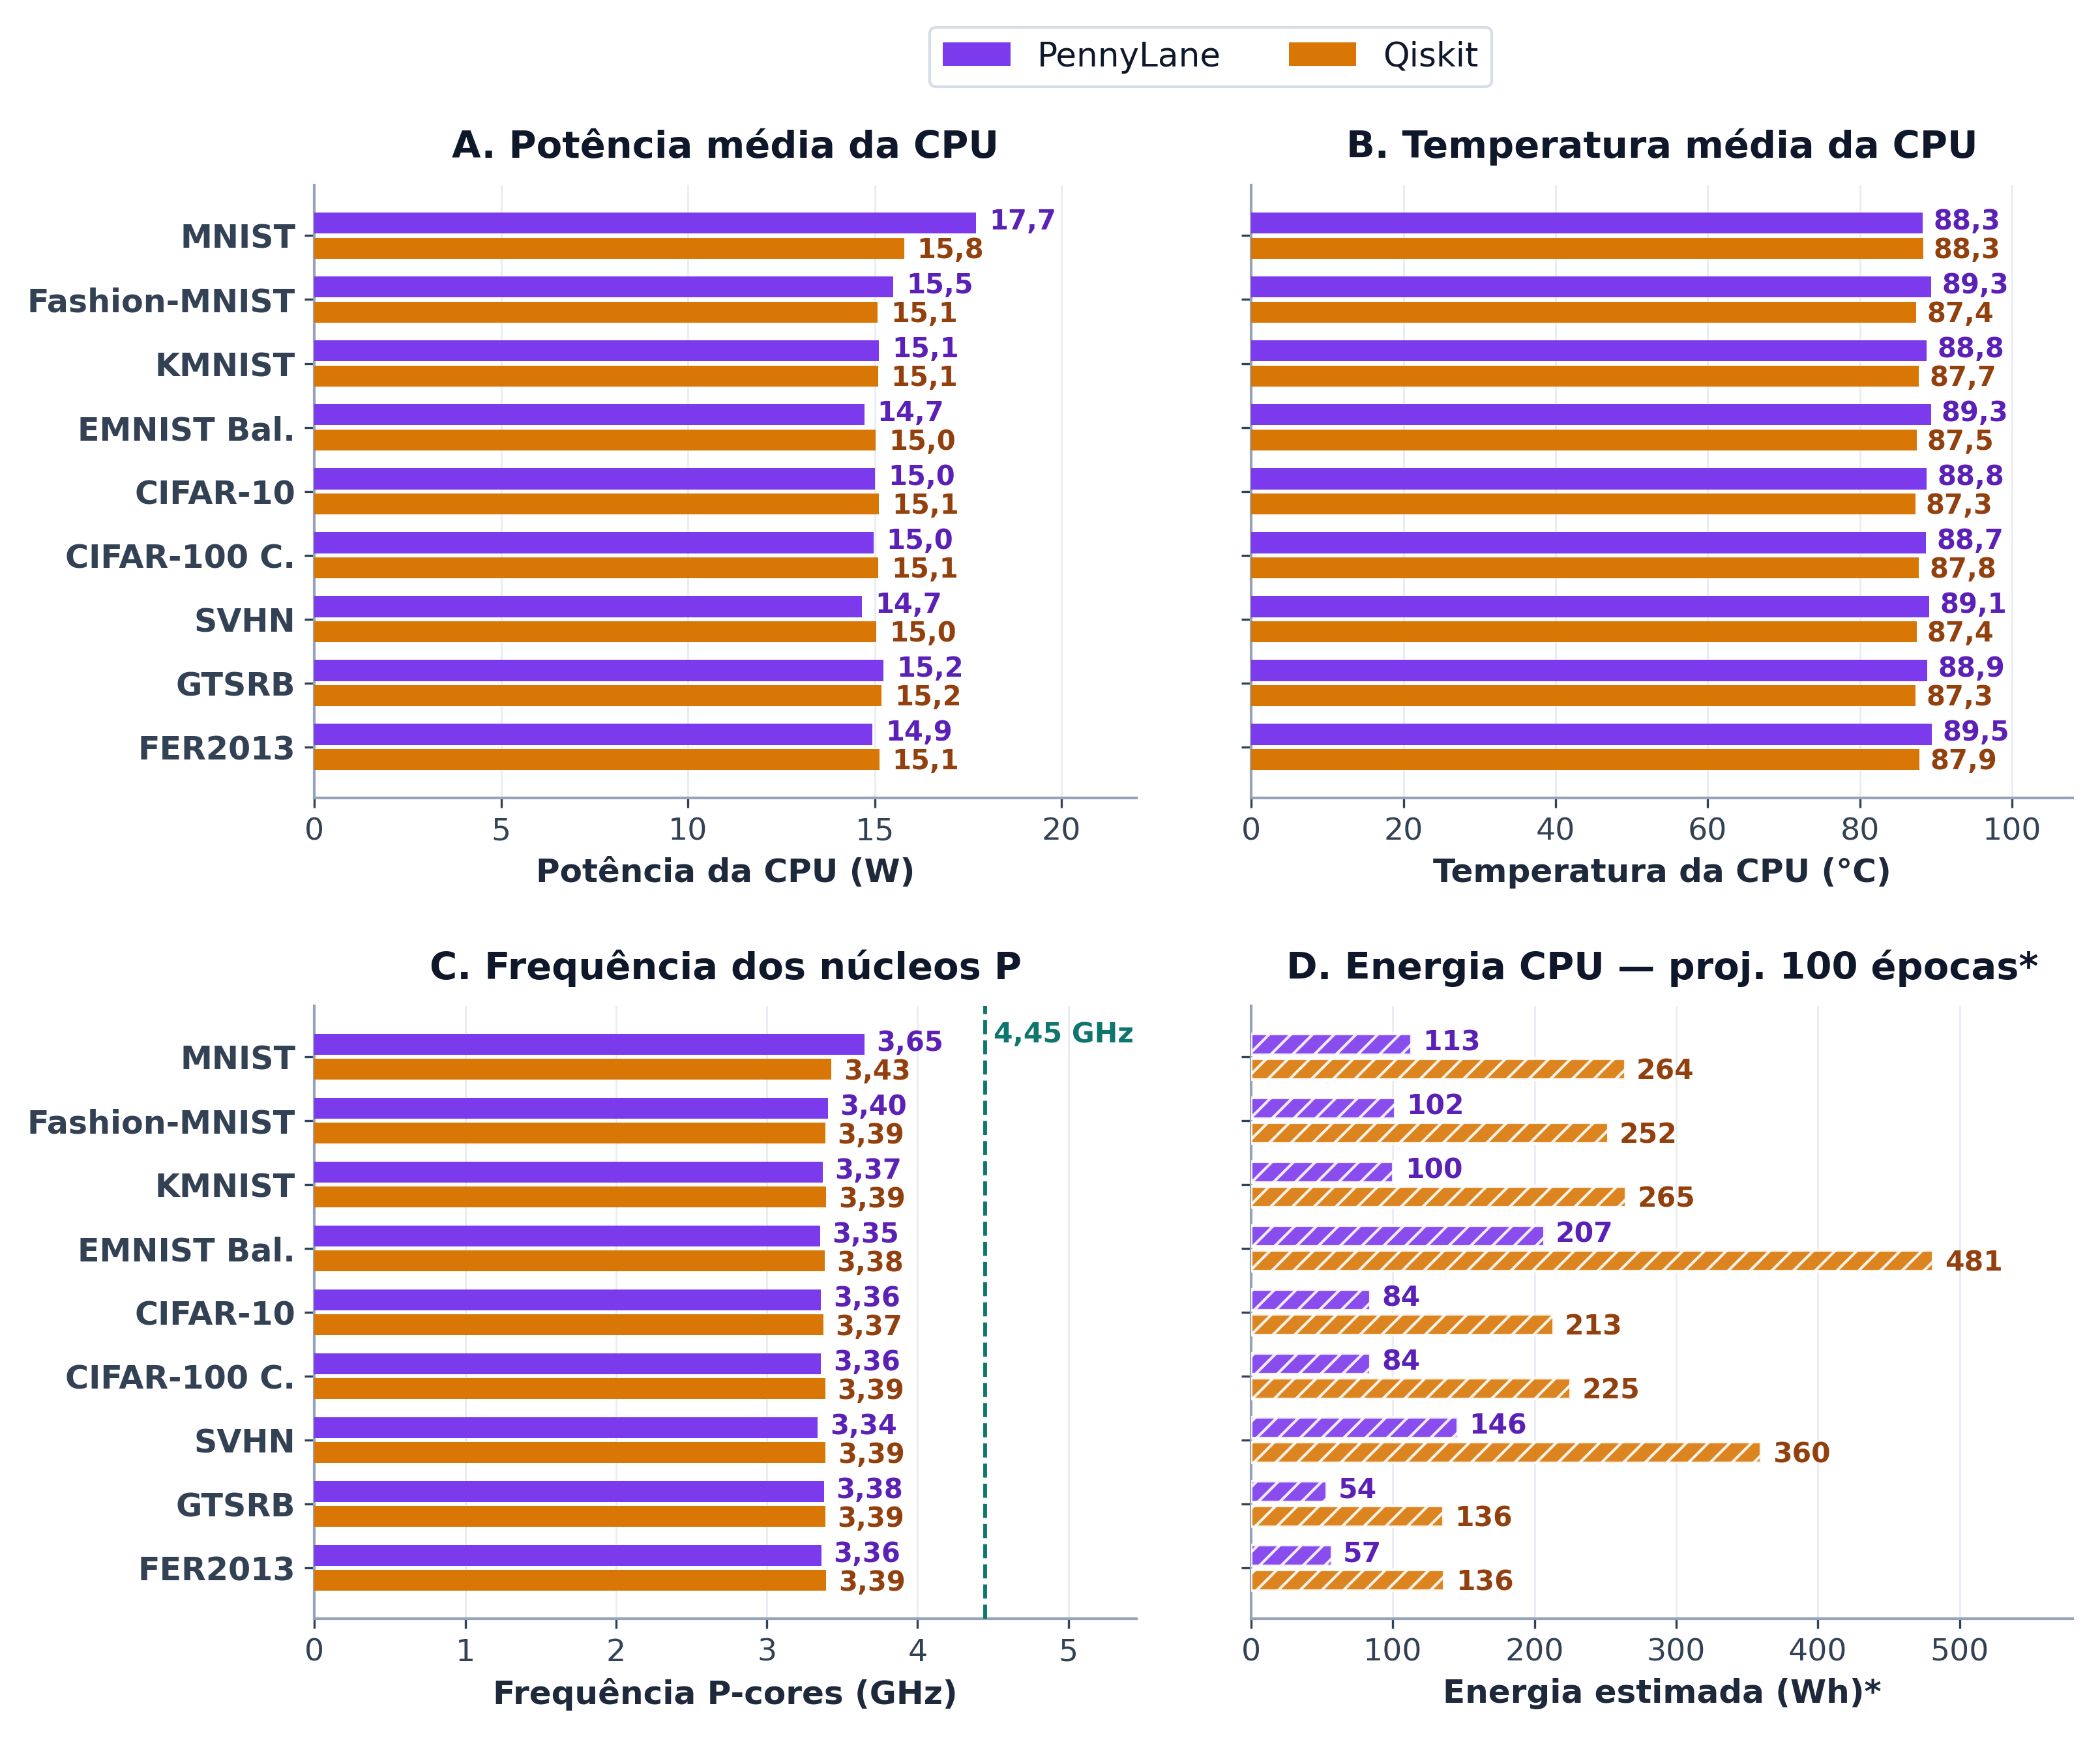
\includegraphics[width=\textwidth,height=0.70\textheight,keepaspectratio]{fig_48_mac_hardware_sensores_macmon.png}
    \end{column}
    \begin{column}{0.39\textwidth}
      \begin{block}{Perfil eletrotérmico (M4)}
        \begin{itemize}\setlength{\itemsep}{5pt}
          \item \textbf{Potência CPU:} 15,22 W (PL) vs.\ 15,15 W (QK); GPU $\approx 0{,}00$ W
          \item \textbf{Térmica / clock:} 89,0~$^\circ$C / 87,6~$^\circ$C; P-cores estáveis em 3,39 GHz (vs.\ 4,45 GHz clássico)
          \item \textcolor{okgreen}{\textbf{Energia (100 ép.*):}} 946,7 Wh (PL) vs.\ 2.332,7 Wh (QK) --- economia projetada de 2,46$\times$
        \end{itemize}
      \end{block}
    \end{column}
  \end{columns}
  \fonte{Elaborado pelo autor (2026).}
\end{frame}

% 47 - TELEMETRIA COMPLEMENTAR NO iMac M4
\begin{frame}{Telemetria complementar no iMac M4 (27 sessões, 1 ép.)}
  \begin{columns}[T,onlytextwidth]
    \begin{column}{0.63\textwidth}
      \centering
      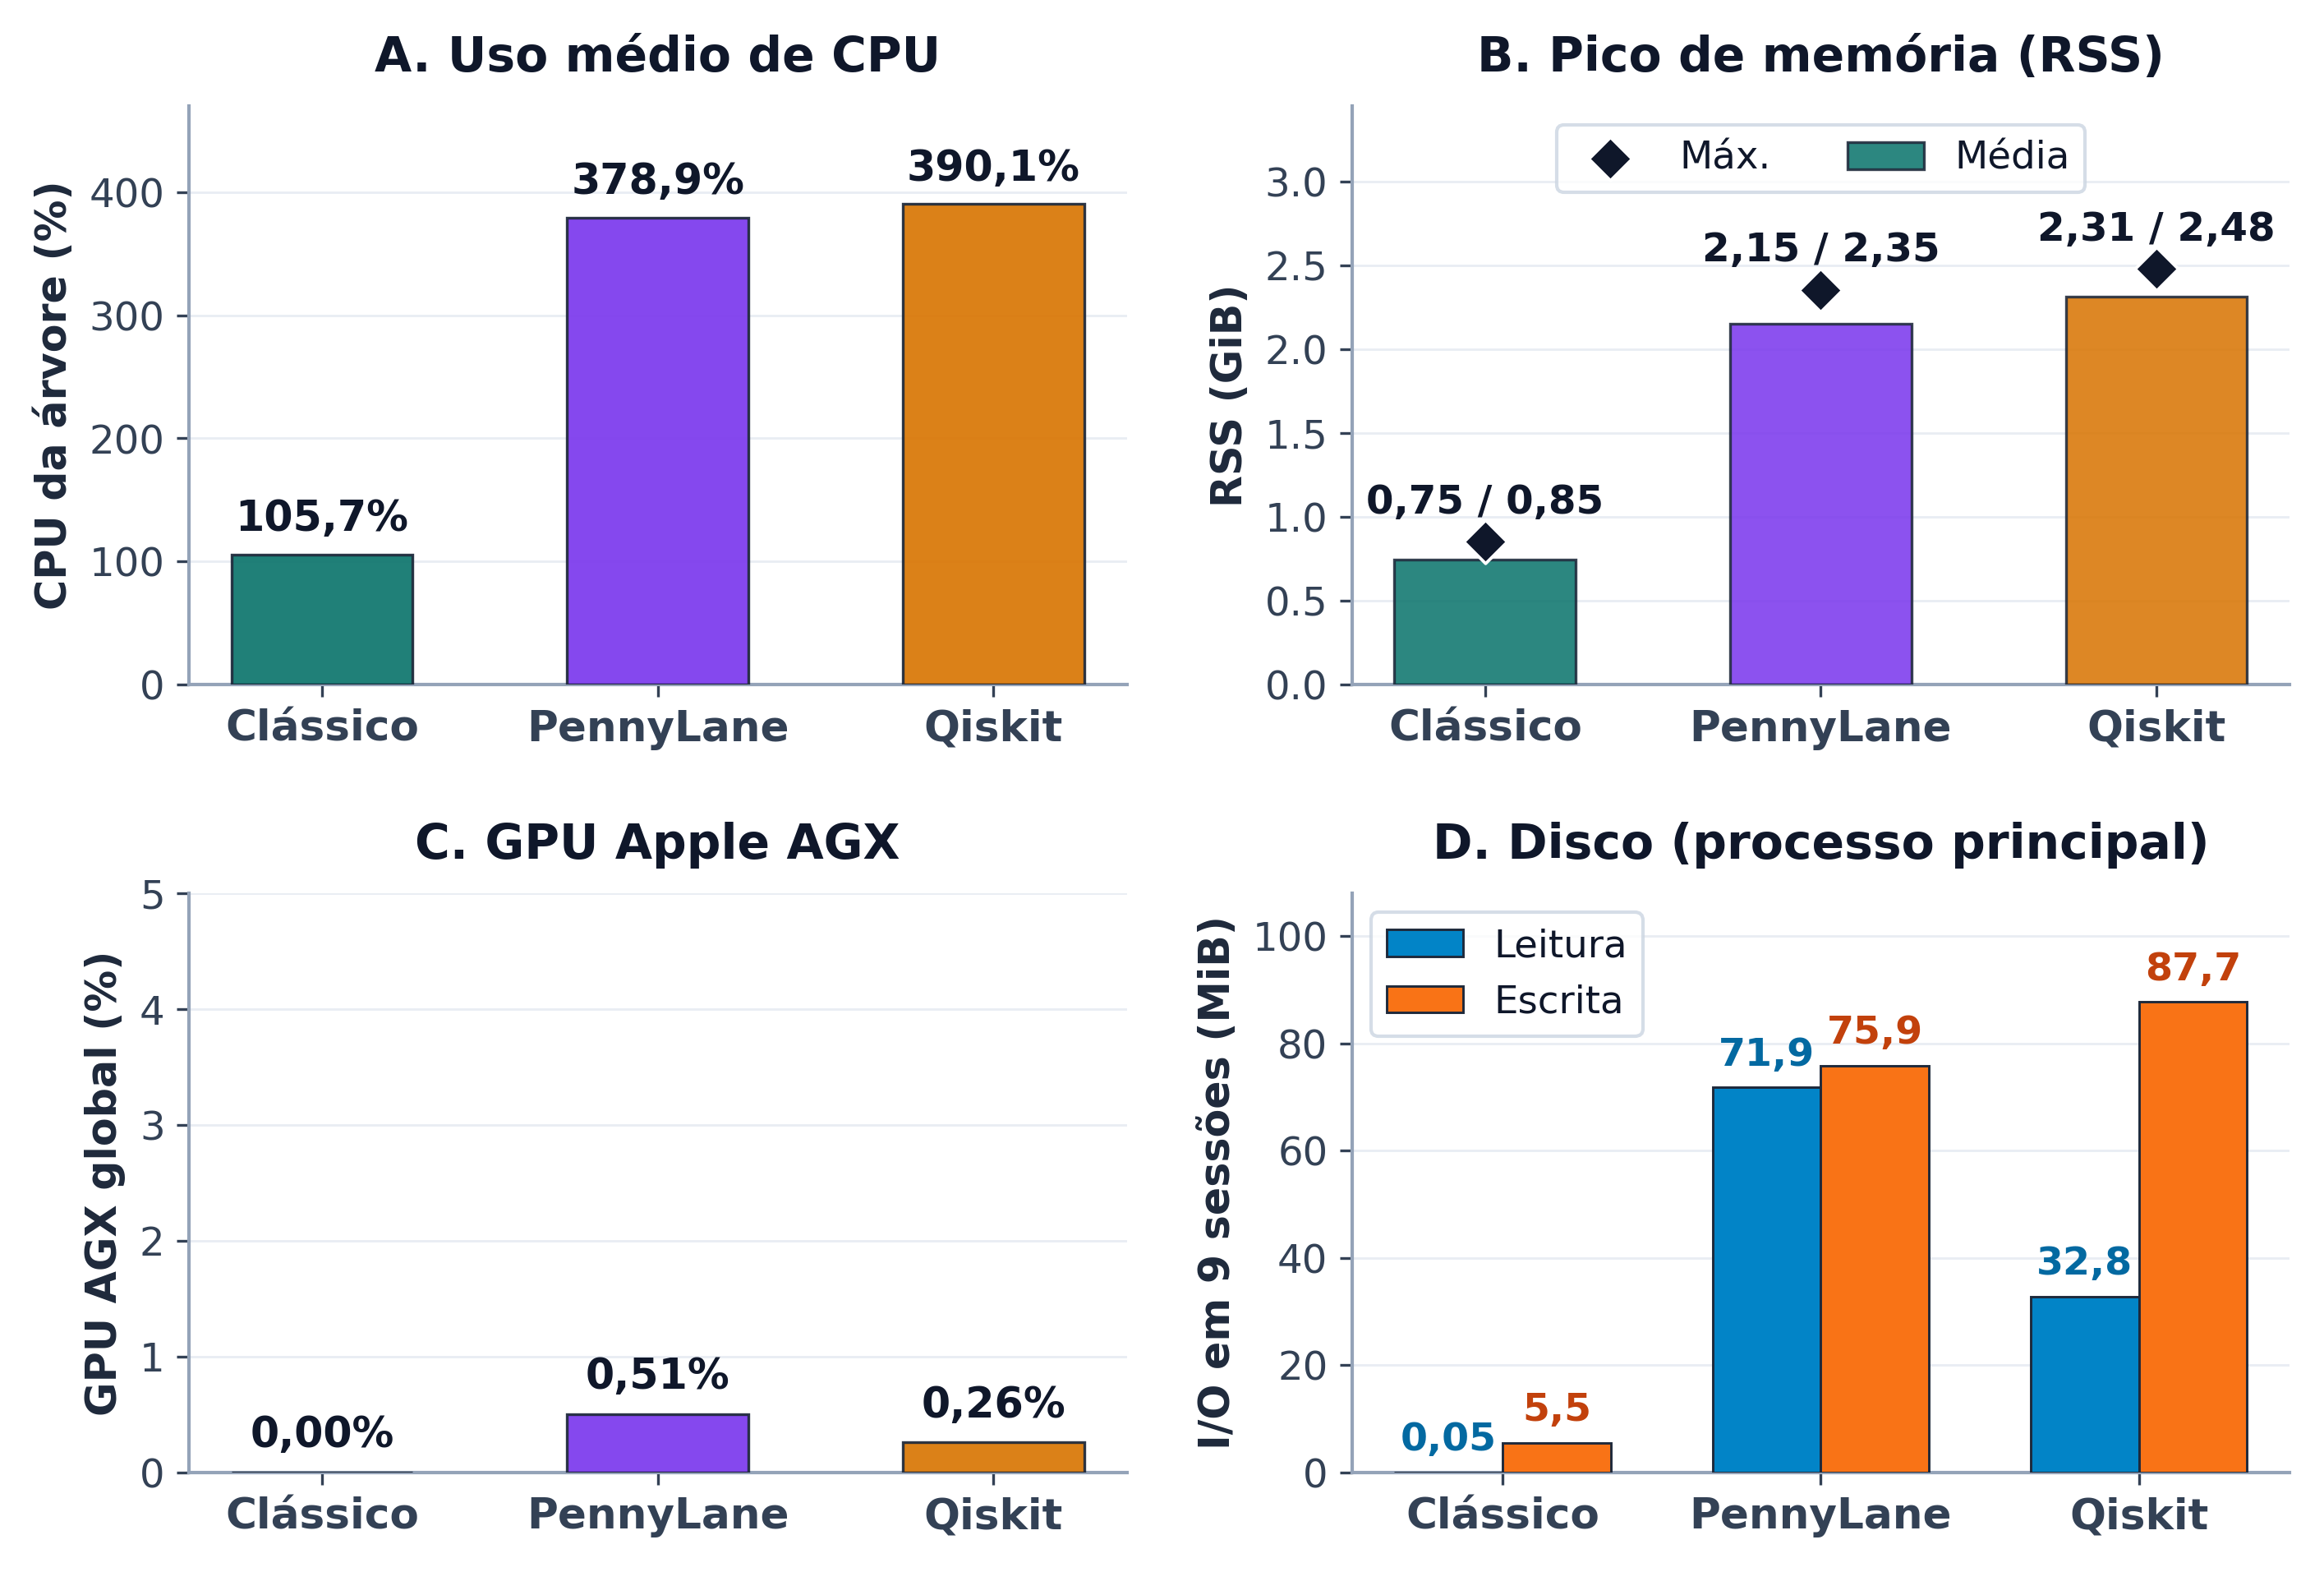
\includegraphics[width=\textwidth,height=0.70\textheight,keepaspectratio]{fig_48_mac_hardware_io_complementar.png}
    \end{column}
    \begin{column}{0.35\textwidth}
      \begin{block}{Confirmado no Apple M4}
        \begin{itemize}\setlength{\itemsep}{4pt}
          \item \textbf{100\% em CPU:} GPU Apple AGX em 0,00\%--0,51\% (potência $\le 0{,}03$ W)
          \item \textbf{Regime \texttt{macmon}:} $\sim 15{,}2$ W CPU, 87,6--89,0~$^\circ$C, P-cores em 3,39 GHz
          \item \textcolor{okgreen}{\textbf{I/O baixo:}} 32$\times$--71$\times$ menos leitura projetada que Windows
          \item \textcolor{okgreen}{\textbf{Energia (100 ép.*):}} PL 0,95 kWh vs.\ QK 2,33 kWh (2,46$\times$ economia)
        \end{itemize}
      \end{block}
    \end{column}
  \end{columns}
  \fonte{Elaborado pelo autor (2026).}
\end{frame}

% 47a - TEMPO ATÉ best.keras VS. 100 ÉPOCAS E MELHOR ÉPOCA (72 MODELOS)
\begin{frame}{Tempo até \texttt{best.keras} vs.\ 100 épocas e melhor época}
  \centering
  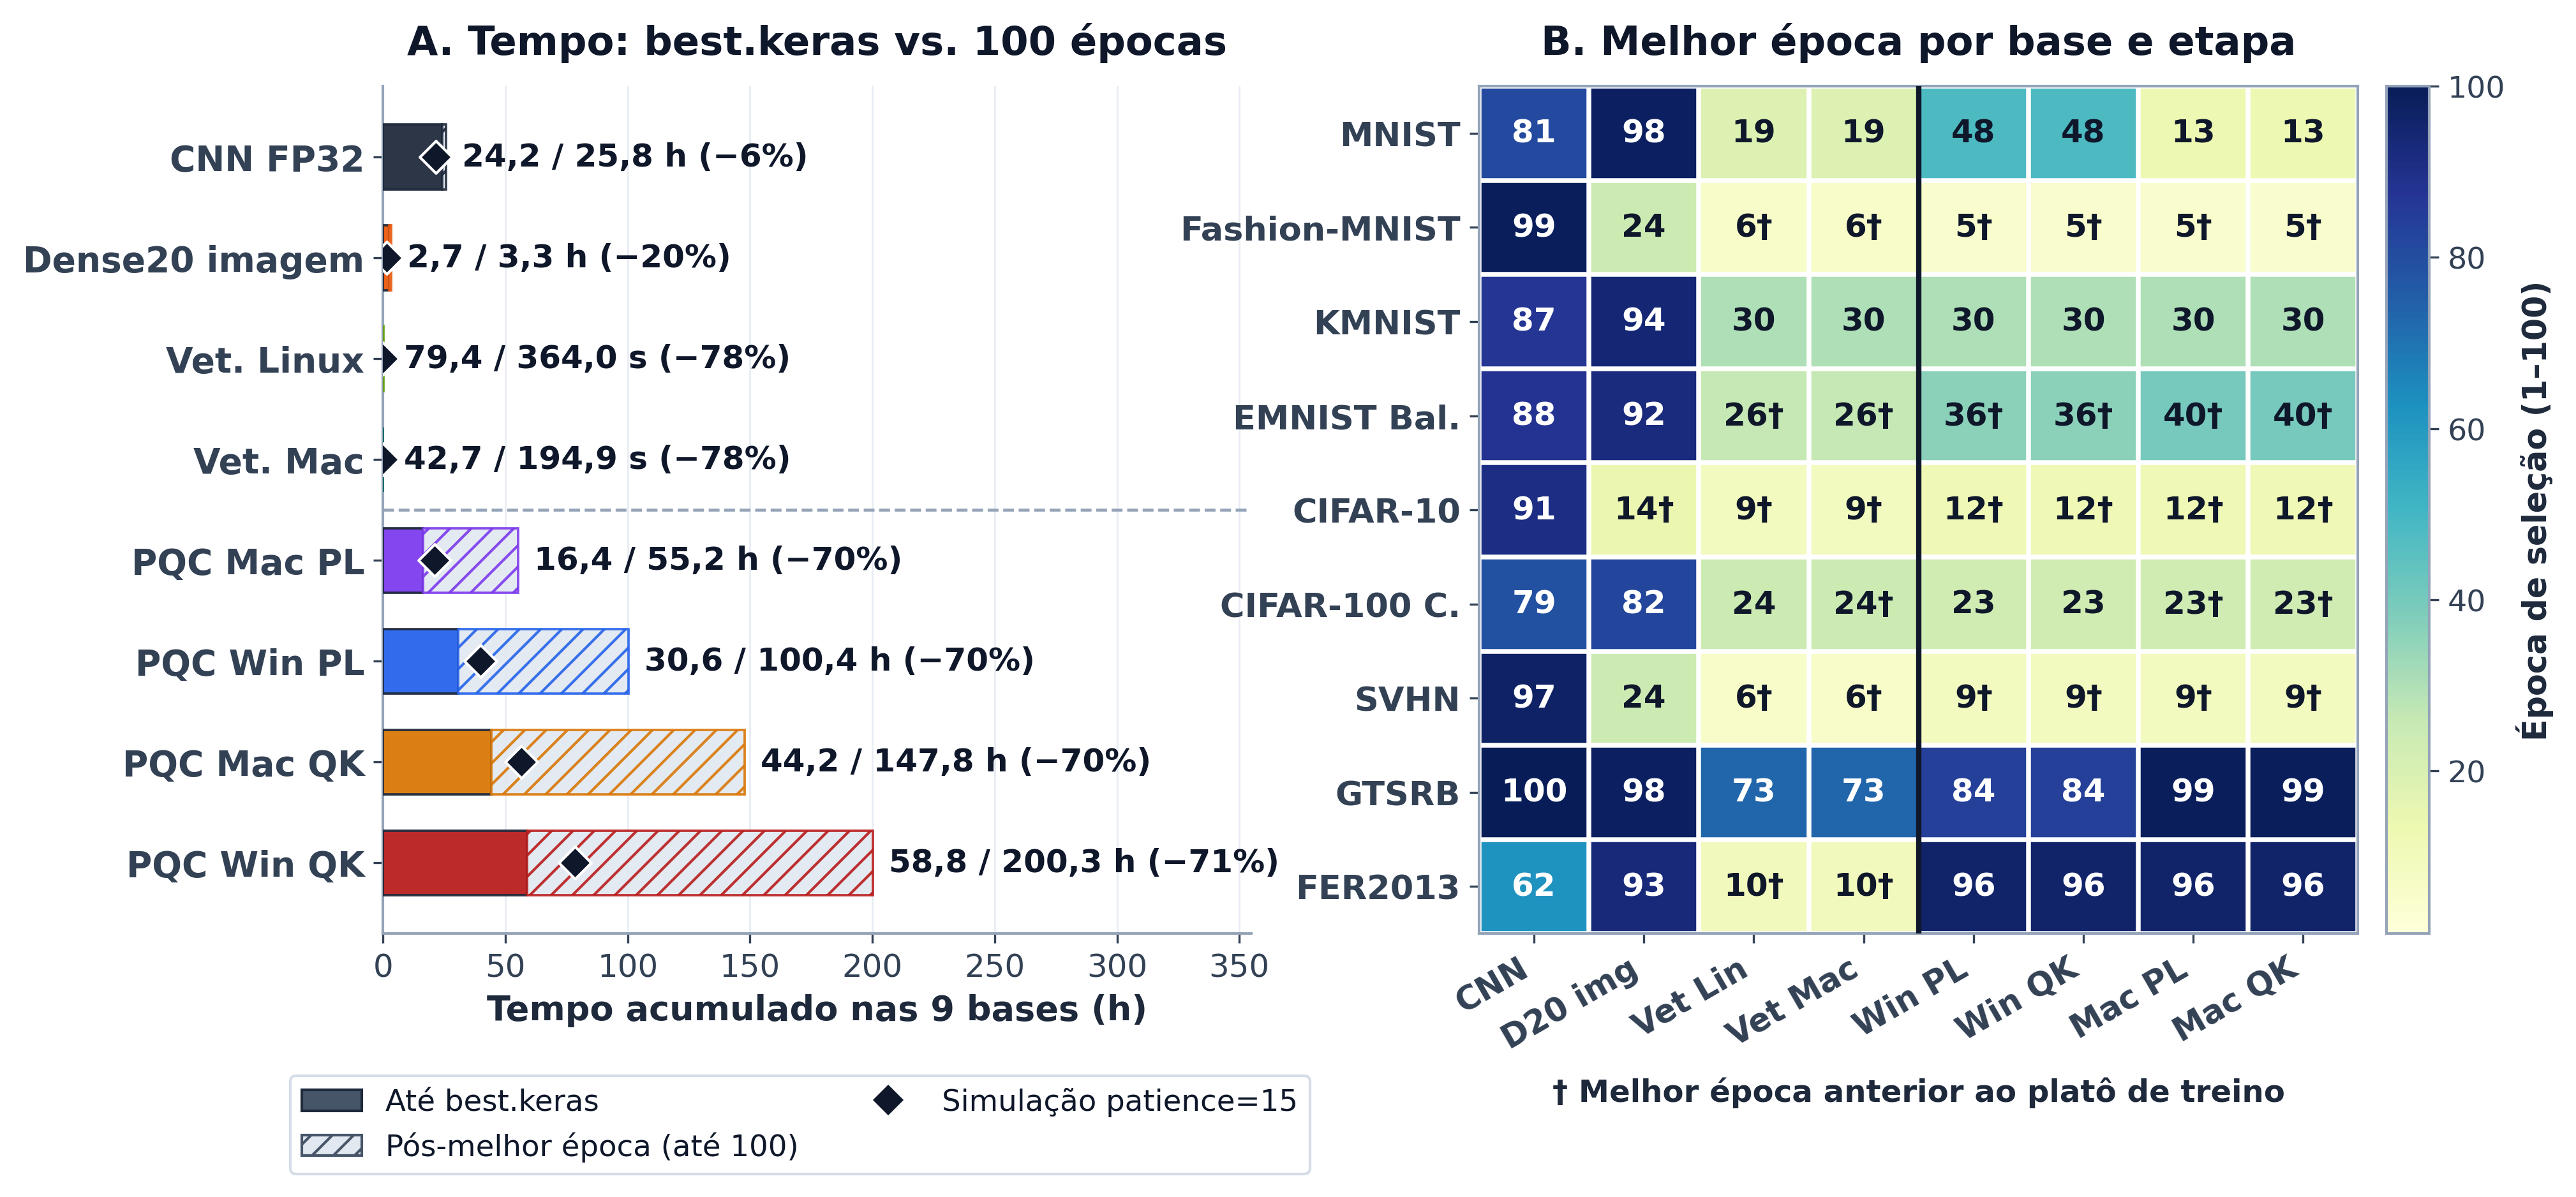
\includegraphics[width=\textwidth,height=0.65\textheight,keepaspectratio]{slides/fig_48_tempo_100ep_vs_melhor_epoca_slide.png}
  \vspace{0.04cm}

  {\footnotesize\color{senacblue}\textbf{72 modelos:} 532,9$\to$177,0~h até \texttt{best.keras} ($-66{,}8\%$; med.\ $e^*=30$) \,|\, \textbf{36 híbridos:} 503,7$\to$150,0~h ($-70{,}2\%$) vs.\ CNN 24,2/25,8~h ($-6\%$).}
  \fonte{Elaborado pelo autor (2026).}
\end{frame}

% 47b - TRAJETÓRIAS TEMPORAIS DE MACRO-F1 (CNN FP32 VS. PQCS - ZOOM)
\begin{frame}{Trajetórias temporais de Macro-F1: CNN FP32 vs.\ PQCs}
  \centering
  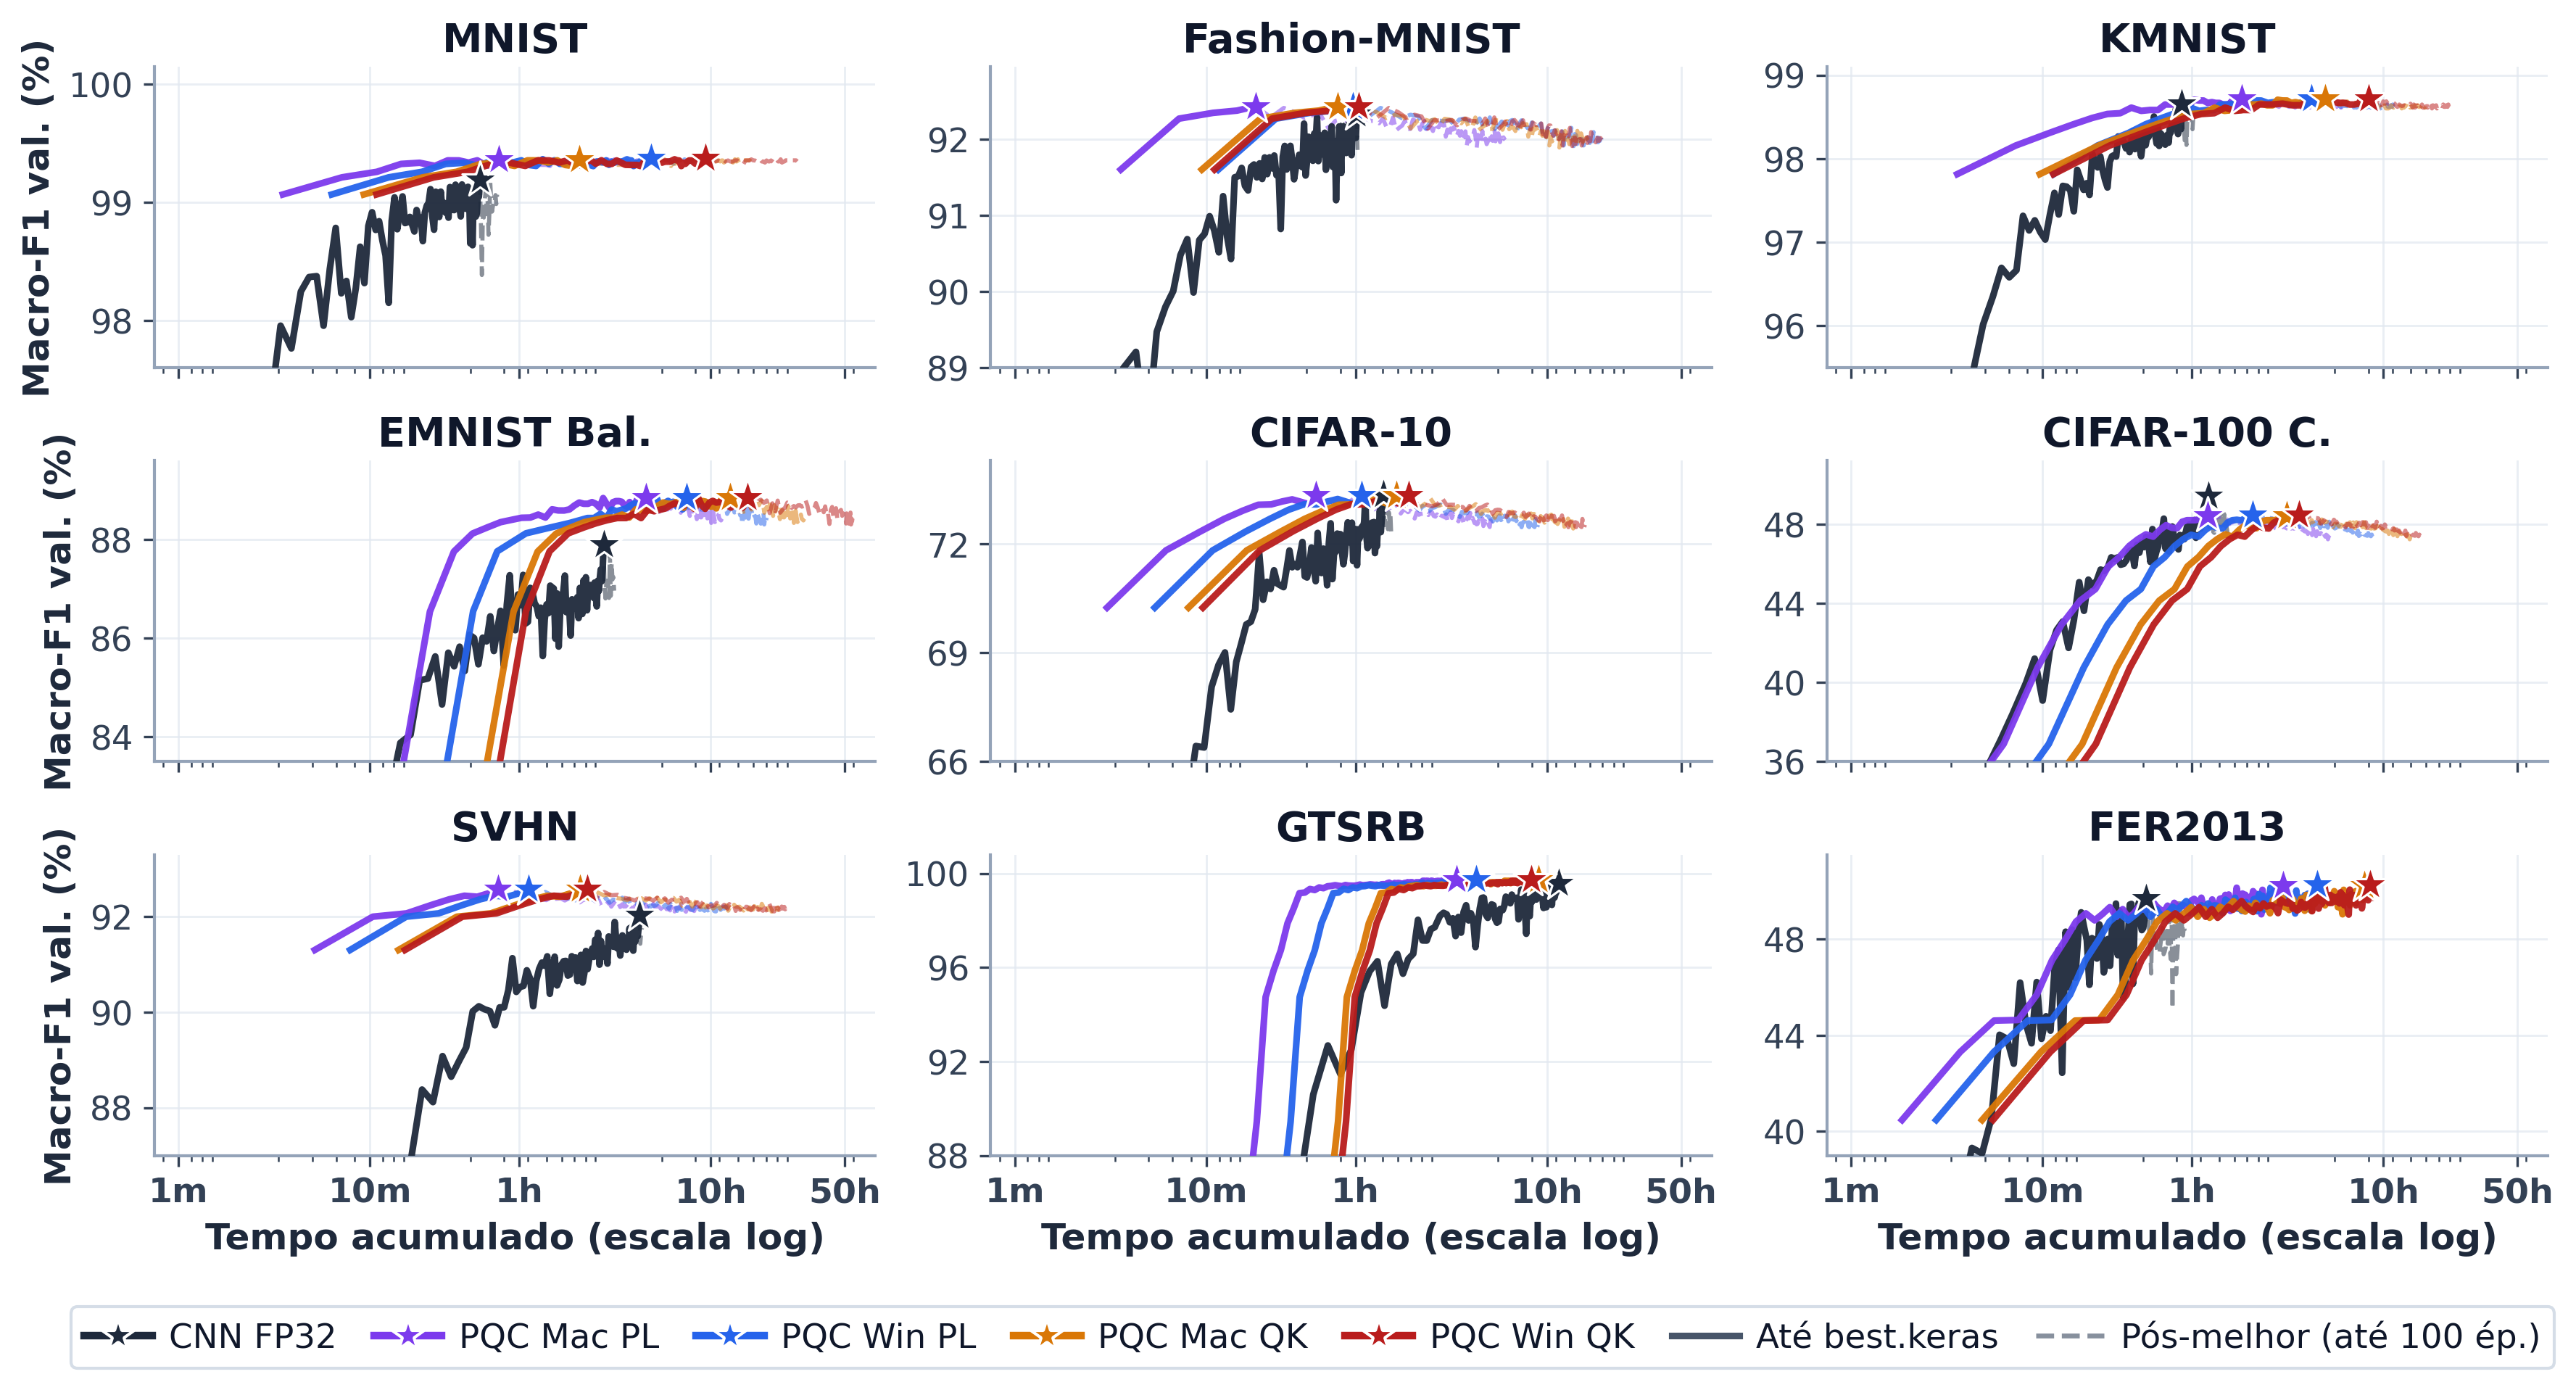
\includegraphics[width=\textwidth,height=0.76\textheight,keepaspectratio]{fig_48_metricas_por_tempo_cnn_pqc.png}
  \fonte{Elaborado pelo autor (2026). Recorte ampliado no platô superior de convergência.}
\end{frame}

% 47c - CUSTO ATÉ best.keras E PARADA ANTECIPADA (CNN FP32 VS. PQCS - ZOOM)
\begin{frame}{Custo até \texttt{best.keras} e \textit{patience}=15: CNN FP32 vs.\ PQCs}
  \centering
  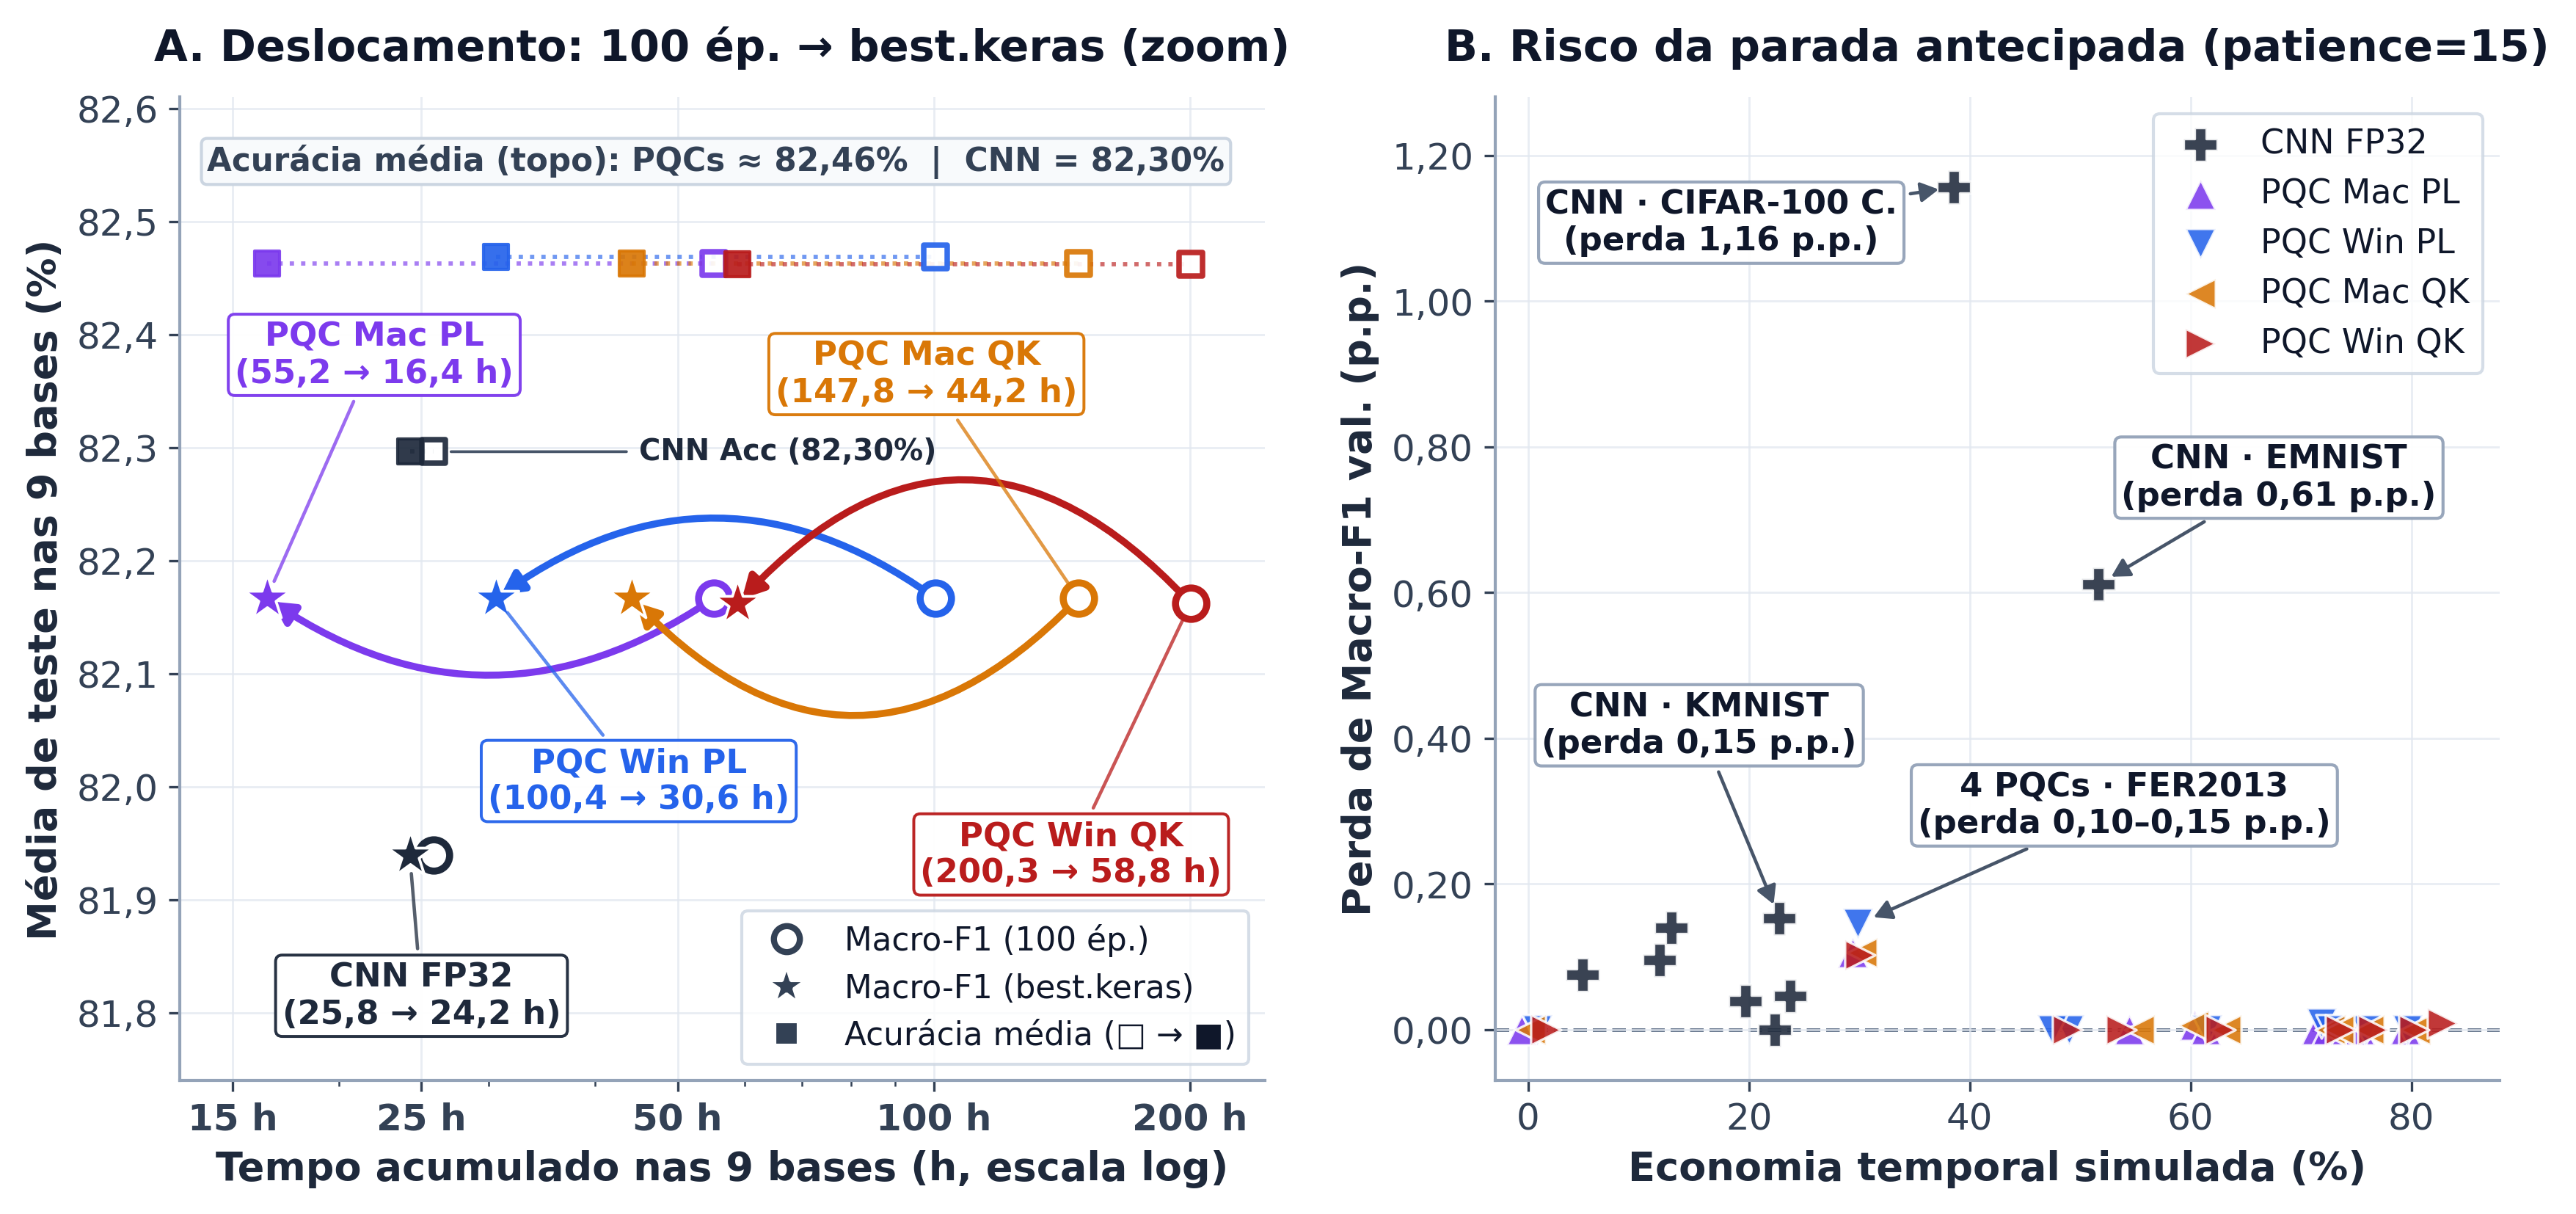
\includegraphics[width=\textwidth,height=0.65\textheight,keepaspectratio]{fig_48_eficiencia_melhor_epoca_patience15_cnn_pqc.png}
  \vspace{0.04cm}

  {\footnotesize\color{senacblue}\textbf{Até \texttt{best.keras}:} PQCs caem $\sim 70\%$ (16,4--58,8~h) vs.\ CNN 24,2~h ($-6\%$); \textit{patience}=15 preserva 28/36 PQCs (máx.\ 0,15~p.p.\ FER2013) frente a 8/9 CNN (até 1,16~p.p.).}
  \fonte{Elaborado pelo autor (2026).}
\end{frame}

% 48 - SÍNTESE
\begin{frame}{Síntese: o que a hipótese e os dados dizem}
  \footnotesize
  \begin{itemize}\setlength{\itemsep}{6pt}
    \item[\ok] Estabilidade nas 9 bases (7 a 47 classes): médias globais entre 81,94\% e 82,23\%
    \item[\ok] Paridade preditiva: $\Delta$ Híb.\ $-$ \texttt{Dense20} de $-0{,}449$ a $+0{,}620$ p.p.; PL vs.\ QK $< 0{,}05$ p.p.
    \item[\ok] Sem vantagem quântica: ganho sobre a CNN vem do gargalo \texttt{Dense20}
    \item[\nok] Trade-offs críticos: custo 778$\times$--2.854$\times$ maior, ECE 36,62\% no FER2013 e $\rho = 0{,}002$
  \end{itemize}
  \vspace{0.2cm}
  \begin{block}{Comparação operacional e literatura}
    Com \texttt{features128}, o híbrido mantém alta separabilidade onde NNQE (filtro fixo) caiu para 36,0\% (CIFAR-10) e 73,4\% (GTSRB). Entre híbridos, PQC Mac PennyLane (55,17 h) lidera; no geral, \texttt{Dense20} vetorial Mac entrega paridade em 194,86 s.
  \end{block}
\end{frame}

% 49 - CONCLUSÃO: RETOMADA
\begin{frame}{Conclusão: retomada do problema e objetivos}
  \footnotesize
  \begin{itemize}\setlength{\itemsep}{8pt}
    \item \textbf{Campanha integralmente auditada:} 9 bases, 72 checkpoints (mais 36 de balanceamento e 27 de telemetria no iMac M4), avaliados por Macro-F1
    \item \textbf{Circuito de Senokosov et al.\ (2024):} convergência estável e paridade com CNN e \texttt{Dense20}, com gradientes ativos nos 4 ramos de 5 qubits
    \item \textbf{Sem superioridade quântica irrestrita:} sem o controle \texttt{Dense20}, ganhos sobre a CNN seriam falsos positivos
    \item \textbf{Eficiência operacional:} iMac M4 + PennyLane é 3,63$\times$ mais rápido e 2,46$\times$ mais econômico em energia que Win/Mac Qiskit, mas 1.019$\times$ mais lento que \texttt{Dense20} vetorial Mac
  \end{itemize}
\end{frame}

% 50 - CONTRIBUIÇÕES
\begin{frame}{Contribuições para a Computação}
  \footnotesize
  \begin{enumerate}\setlength{\itemsep}{6pt}
    \item \textbf{Benchmark padronizado em 9 bases (72 modelos):} supera recortes binários e cobre as 20 superclasses do CIFAR-100 Coarse em Macro-F1
    \item \textbf{Controle \texttt{Dense20} e contabilidade paramétrica:} evita falsos positivos arquiteturais e separa pesos da cabeça vs.\ inferência completa
    \item \textbf{Auditoria de calibração, Bayes e explicabilidade:} ECE/NLL/Brier, 1.336 posteriores, 576 Grad-CAM e 73.728 oclusões ($\rho = 0{,}002$)
    \item \textbf{Telemetria multiplataforma de hardware e energia:} \textit{speedups} exatos, CPU, RSS, GPU RTX/AGX, I/O e sensores \texttt{macmon} no Apple M4
    \item \textbf{Auditoria crítica de dados e literatura:} \textit{tracks} no GTSRB (67,9\%), duplicatas/conflitos no FER2013 e divergências em artigos
  \end{enumerate}
\end{frame}

% 51 - LIMITAÇÕES E TRABALHOS FUTUROS
\begin{frame}{Limitações e trabalhos futuros}
  \centering
  {\footnotesize
  \begin{tabular}{@{}R{6.2cm}R{7.4cm}@{}}
    \toprule
    \textbf{Limitação auditada} & \textbf{Trabalho futuro prioritário} \\
    \midrule
    Semente única; \textit{tracks} (GTSRB) e duplicatas (FER2013) & Split \textit{track-aware}, deduplicação e múltiplas sementes com IC \\
    Descalibração sobre \textit{features} congeladas (ECE 36,6\%) & Recalibração pós-treino (\textit{temperature scaling}) e \textit{label smoothing} \\
    4 ramos sem emaranhamento; \textit{parameter-shift} em CPU & Emaranhamento cruzado, \textit{data re-uploading}, adjunto e GPU/\textit{cuQuantum} \\
    Capacidade distinta entre \texttt{Dense20} e cabeça híbrida & Ablação de largura do gargalo e pareamento estrito de parâmetros \\
    Apenas simulação ideal local (sem QPU física) & Execução com mitigação de erros em processadores quânticos reais \\
    \bottomrule
  \end{tabular}}
\end{frame}

% 52 - OBRIGADO
{
\setbeamertemplate{footline}{}
\begin{frame}[plain]
  \centering
  \vspace{0.5cm}
  \logosenacgrande
  \vspace{0.6cm}

  {\Huge\bfseries\color{senacblue}Obrigado!\par}
  \vspace{0.3cm}
  {\Large\bfseries\color{senacorange}Perguntas?\par}
  \vspace{0.6cm}
  {\normalsize\bfseries Matheus Sanchez Duda\par}
  \vspace{0.15cm}
  {\footnotesize\color{textmuted}Orientador: Prof. Samuel Mendes Sanches Junior\\
  Coorientador: Prof. Thyago Conchado Quintas\par}
\end{frame}
}

% ===============================================================
% APÊNDICE (A1..A6)
% ===============================================================
\appendix

% A1
\begin{frame}{Apoio A1: sobreamostragem e subamostragem}
  \begin{columns}[T,onlytextwidth]
    \begin{column}{0.48\textwidth}
      \centering
      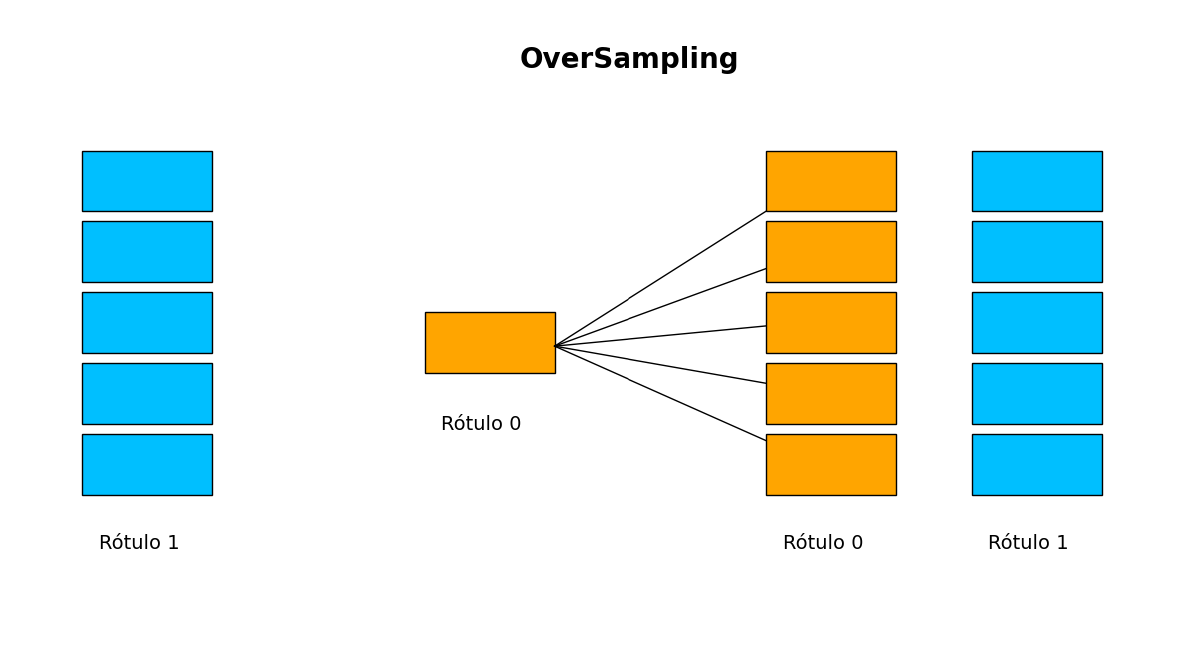
\includegraphics[width=\textwidth,height=0.40\textheight,keepaspectratio]{balanceamento_oversampling_silva2025.png}\\[4pt]
      {\footnotesize\bfseries\color{senacblue}Sobreamostragem (\textit{oversampling})}
    \end{column}
    \begin{column}{0.48\textwidth}
      \centering
      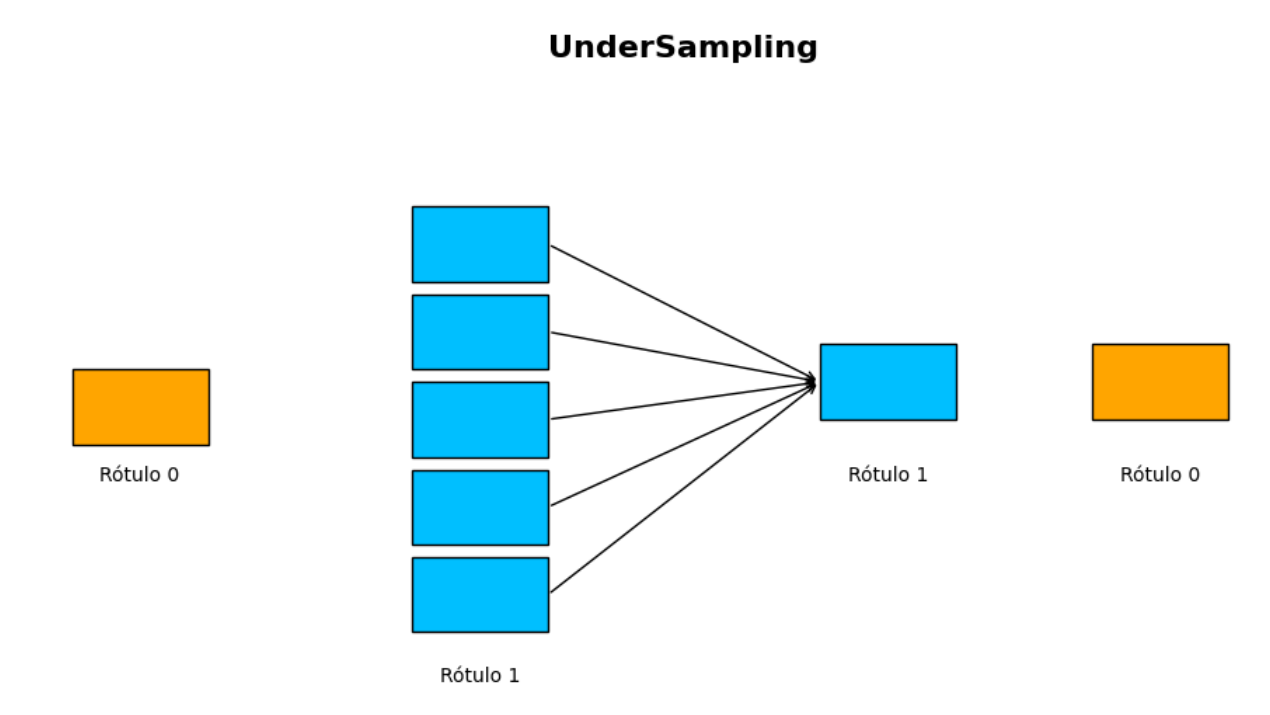
\includegraphics[width=\textwidth,height=0.40\textheight,keepaspectratio]{balanceamento_undersampling_silva2025.png}\\[4pt]
      {\footnotesize\bfseries\color{senacblue}Subamostragem (\textit{undersampling})}
    \end{column}
  \end{columns}
  \vspace{0.2cm}
  \begin{itemize}\footnotesize
    \item Estratégias de dados e de algoritmo (\texttt{class\_weight}) testadas em 36 execuções preliminares
    \item Validação e teste mantêm sempre a distribuição original; avaliação primária em Macro-F1
  \end{itemize}
  \fonte{adaptado de Silva (2025).}
\end{frame}

% A2
\begin{frame}{Apoio A2: calibração probabilística no FER2013}
  \begin{columns}[T,onlytextwidth]
    \begin{column}{0.56\textwidth}
      \centering
      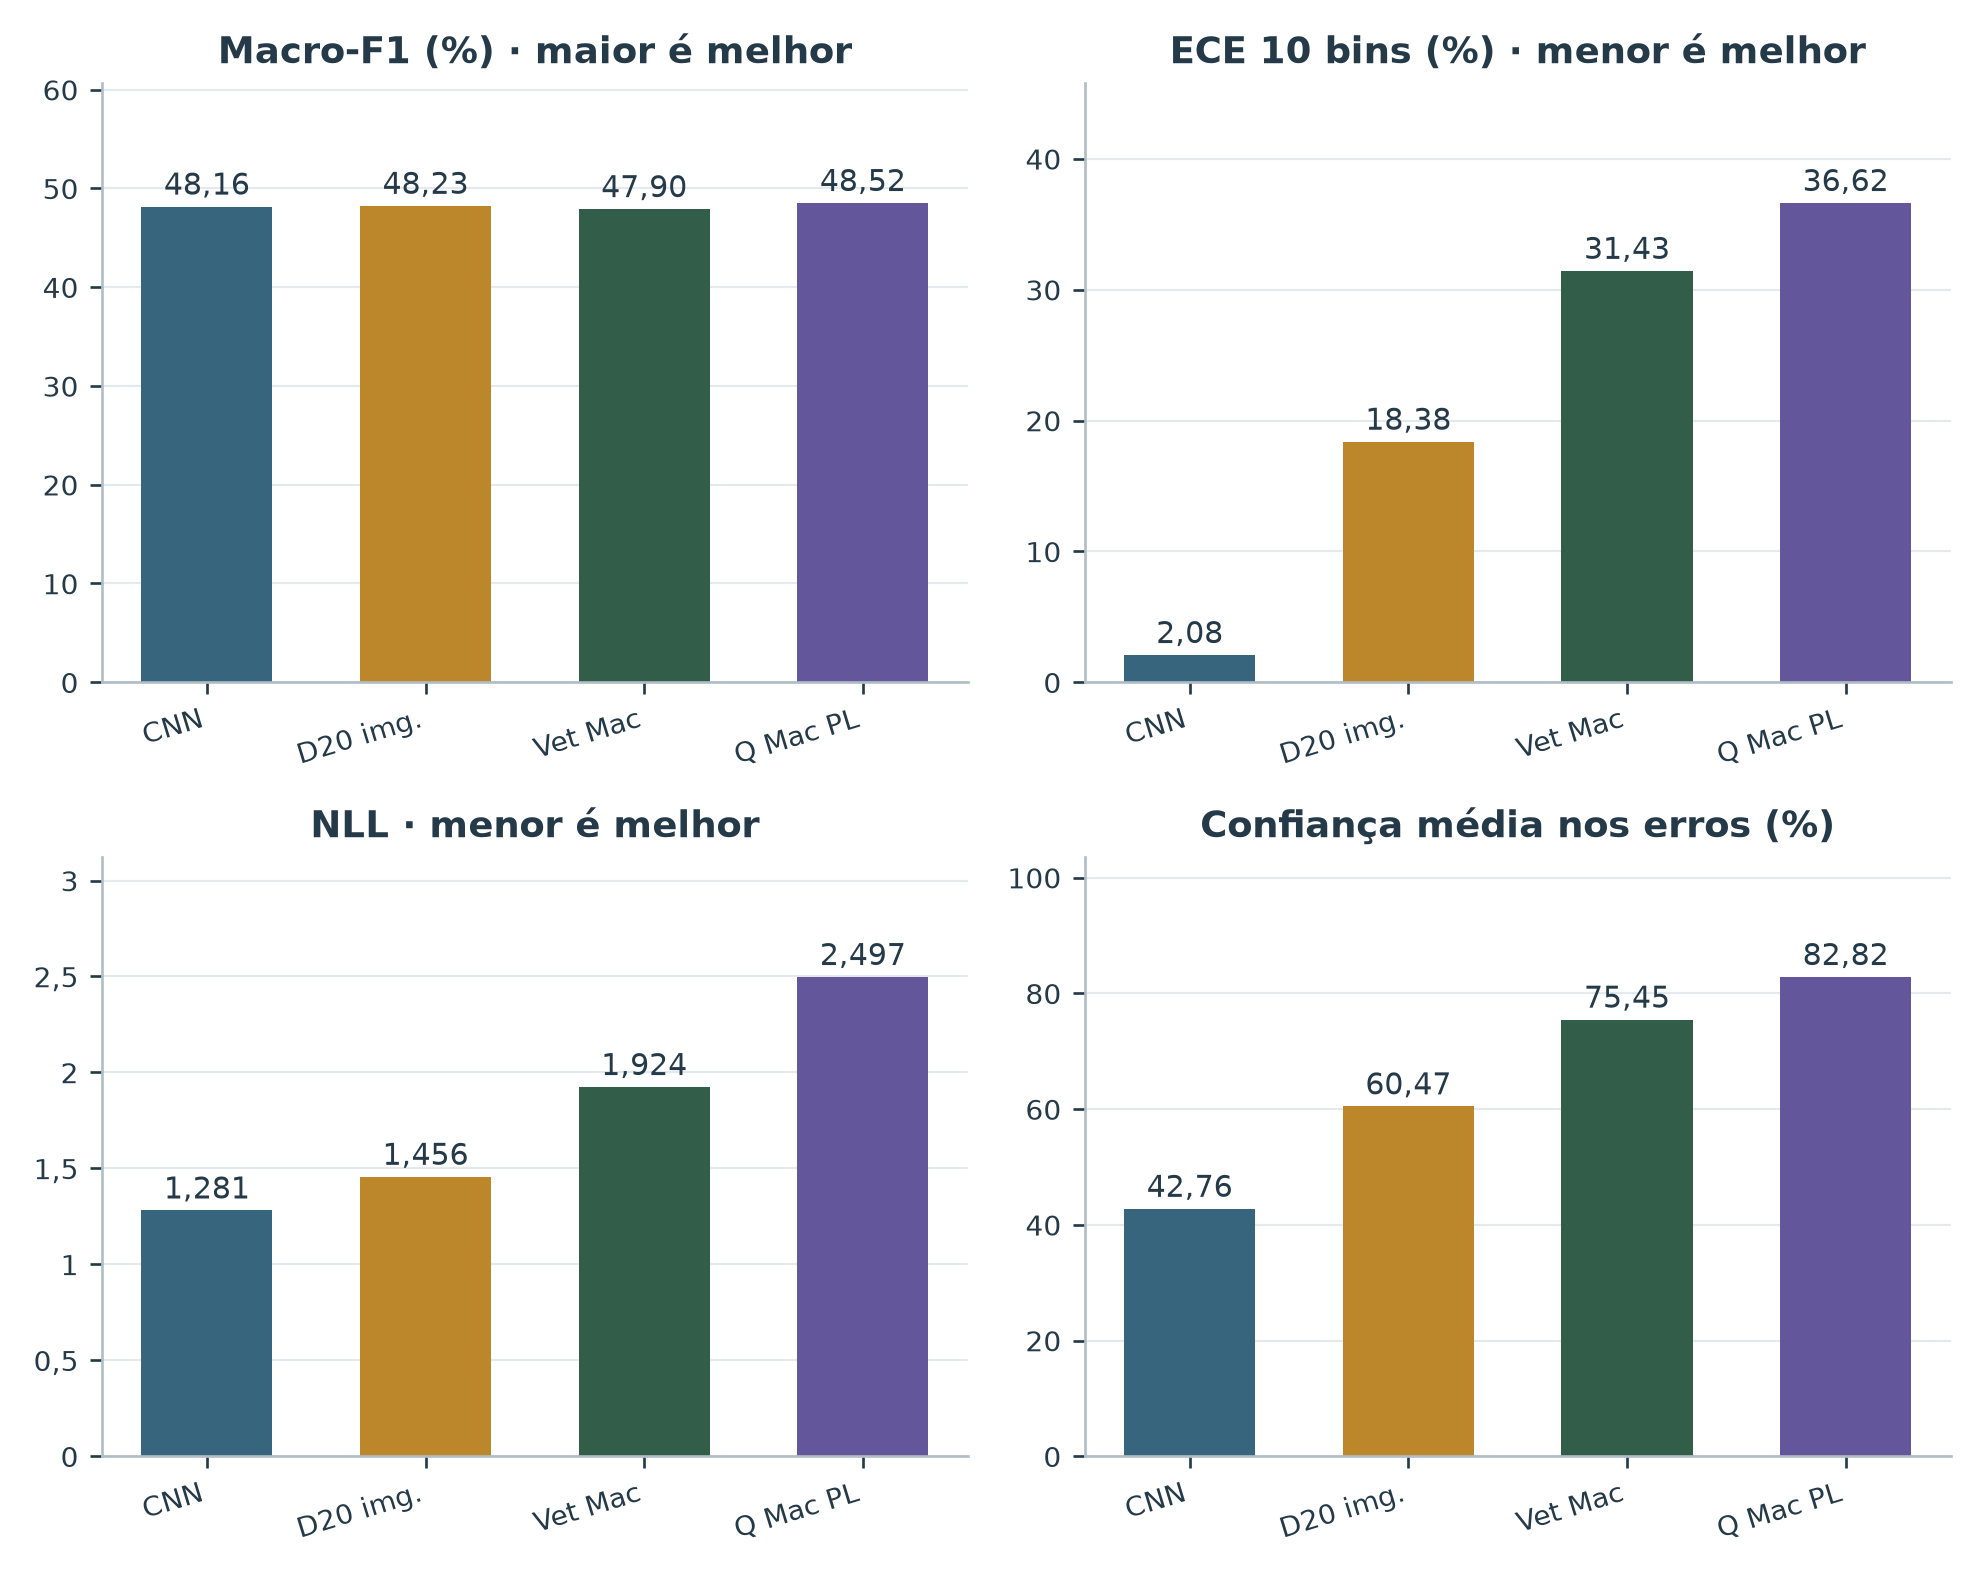
\includegraphics[width=\textwidth,height=0.68\textheight,keepaspectratio]{figura_28_calibracao_fer.png}
    \end{column}
    \begin{column}{0.42\textwidth}
      \begin{block}{Confiança excessiva nos erros}
        \begin{itemize}\setlength{\itemsep}{4pt}
          \item \textcolor{okgreen}{\textbf{CNN FP32 (LS 0,05):}} ECE = 2,08\%, NLL = 1,281, conf.\ nos erros = 42,76\%
          \item \textbf{D20 imagem:} ECE = 18,38\%, erros = 60,47\%
          \item \textbf{Vetorial Mac:} ECE = 31,43\%, erros = 75,45\%
          \item \textcolor{badred}{\textbf{PQC Mac PL:}} ECE = 36,62\%, NLL = 2,497, conf.\ nos erros = 82,82\% (requer \textit{temperature scaling})
        \end{itemize}
      \end{block}
    \end{column}
  \end{columns}
  \fonte{Elaborado pelo autor (2026).}
\end{frame}

% A3
\begin{frame}{Apoio A3: gradientes por ramo e ruído/\textit{shots}}
  \begin{columns}[T,onlytextwidth]
    \begin{column}{0.48\textwidth}
      \centering
      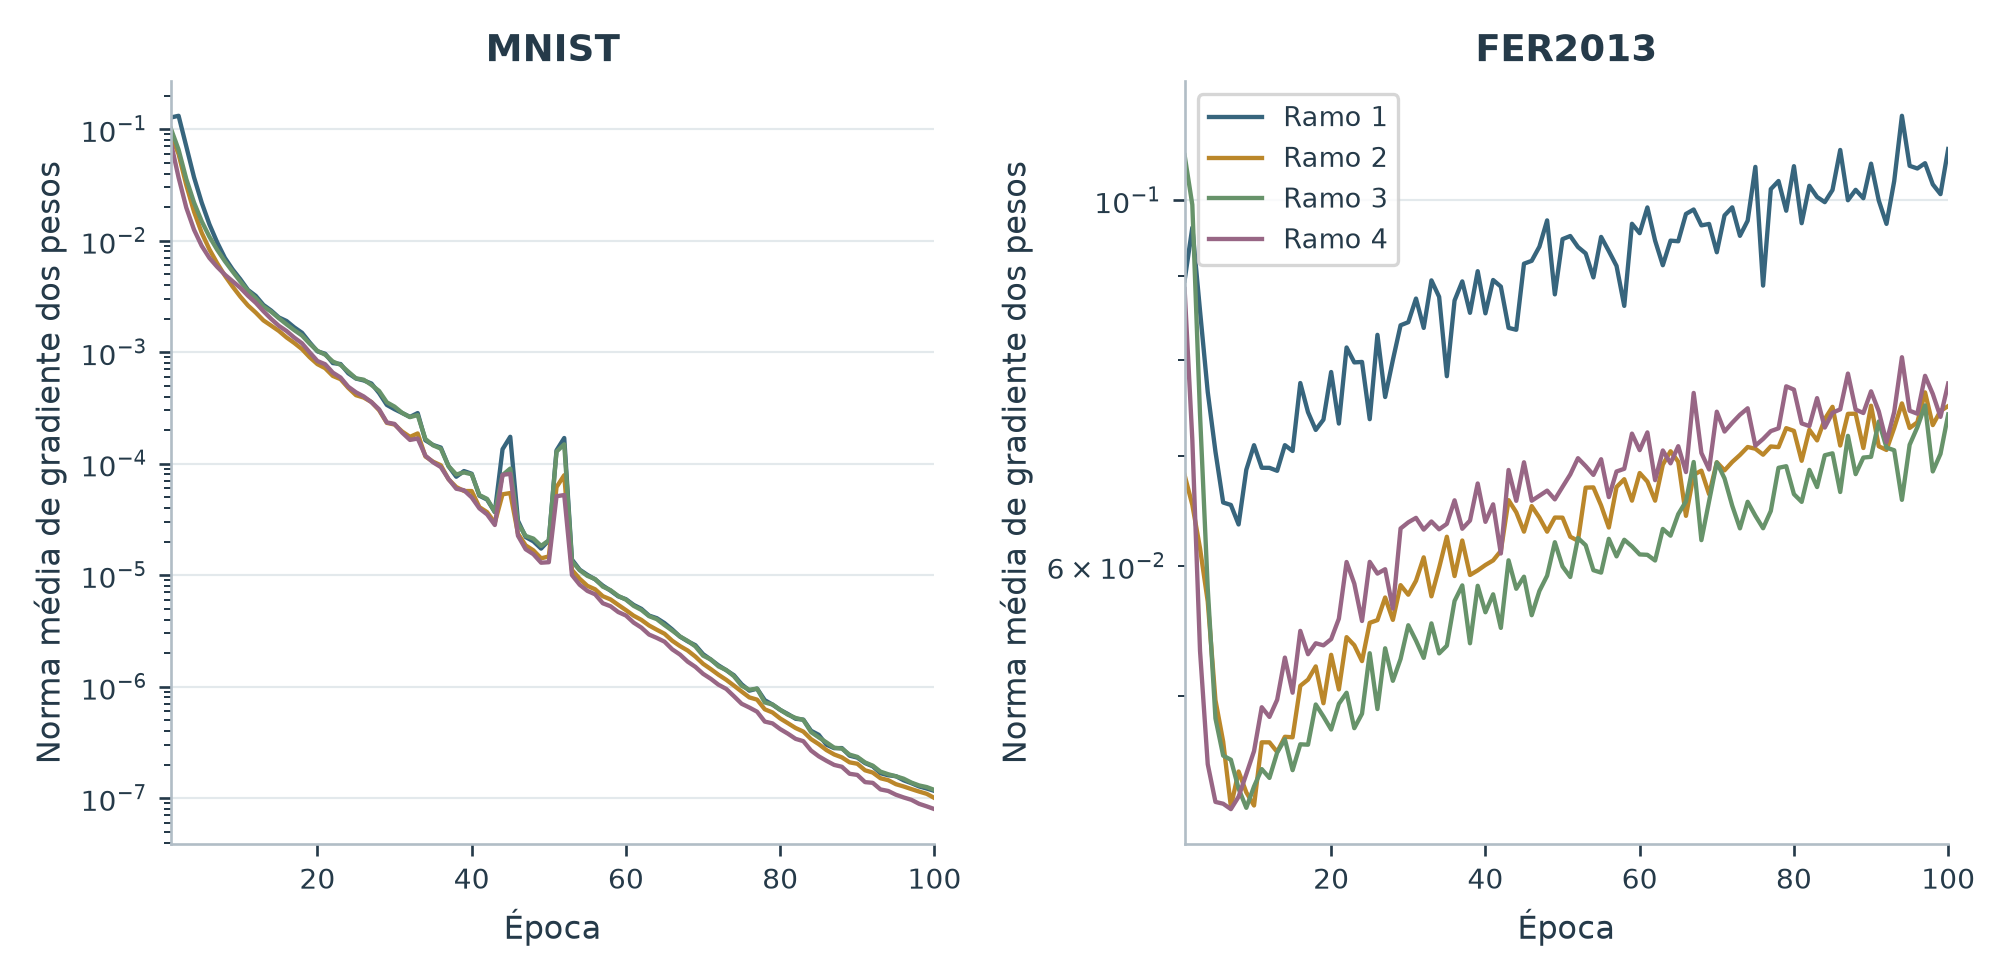
\includegraphics[width=\textwidth,height=0.46\textheight,keepaspectratio]{figura_19_gradientes.png}\\[4pt]
      {\footnotesize Gradientes (Ramos 1--4): MNIST decai ($0{,}13\to 10^{-7}$); FER2013 segue ativo ($4{,}3\times 10^{-2}$ a $1{,}1\times 10^{-1}$) até a época 100.}
    \end{column}
    \begin{column}{0.48\textwidth}
      \centering
      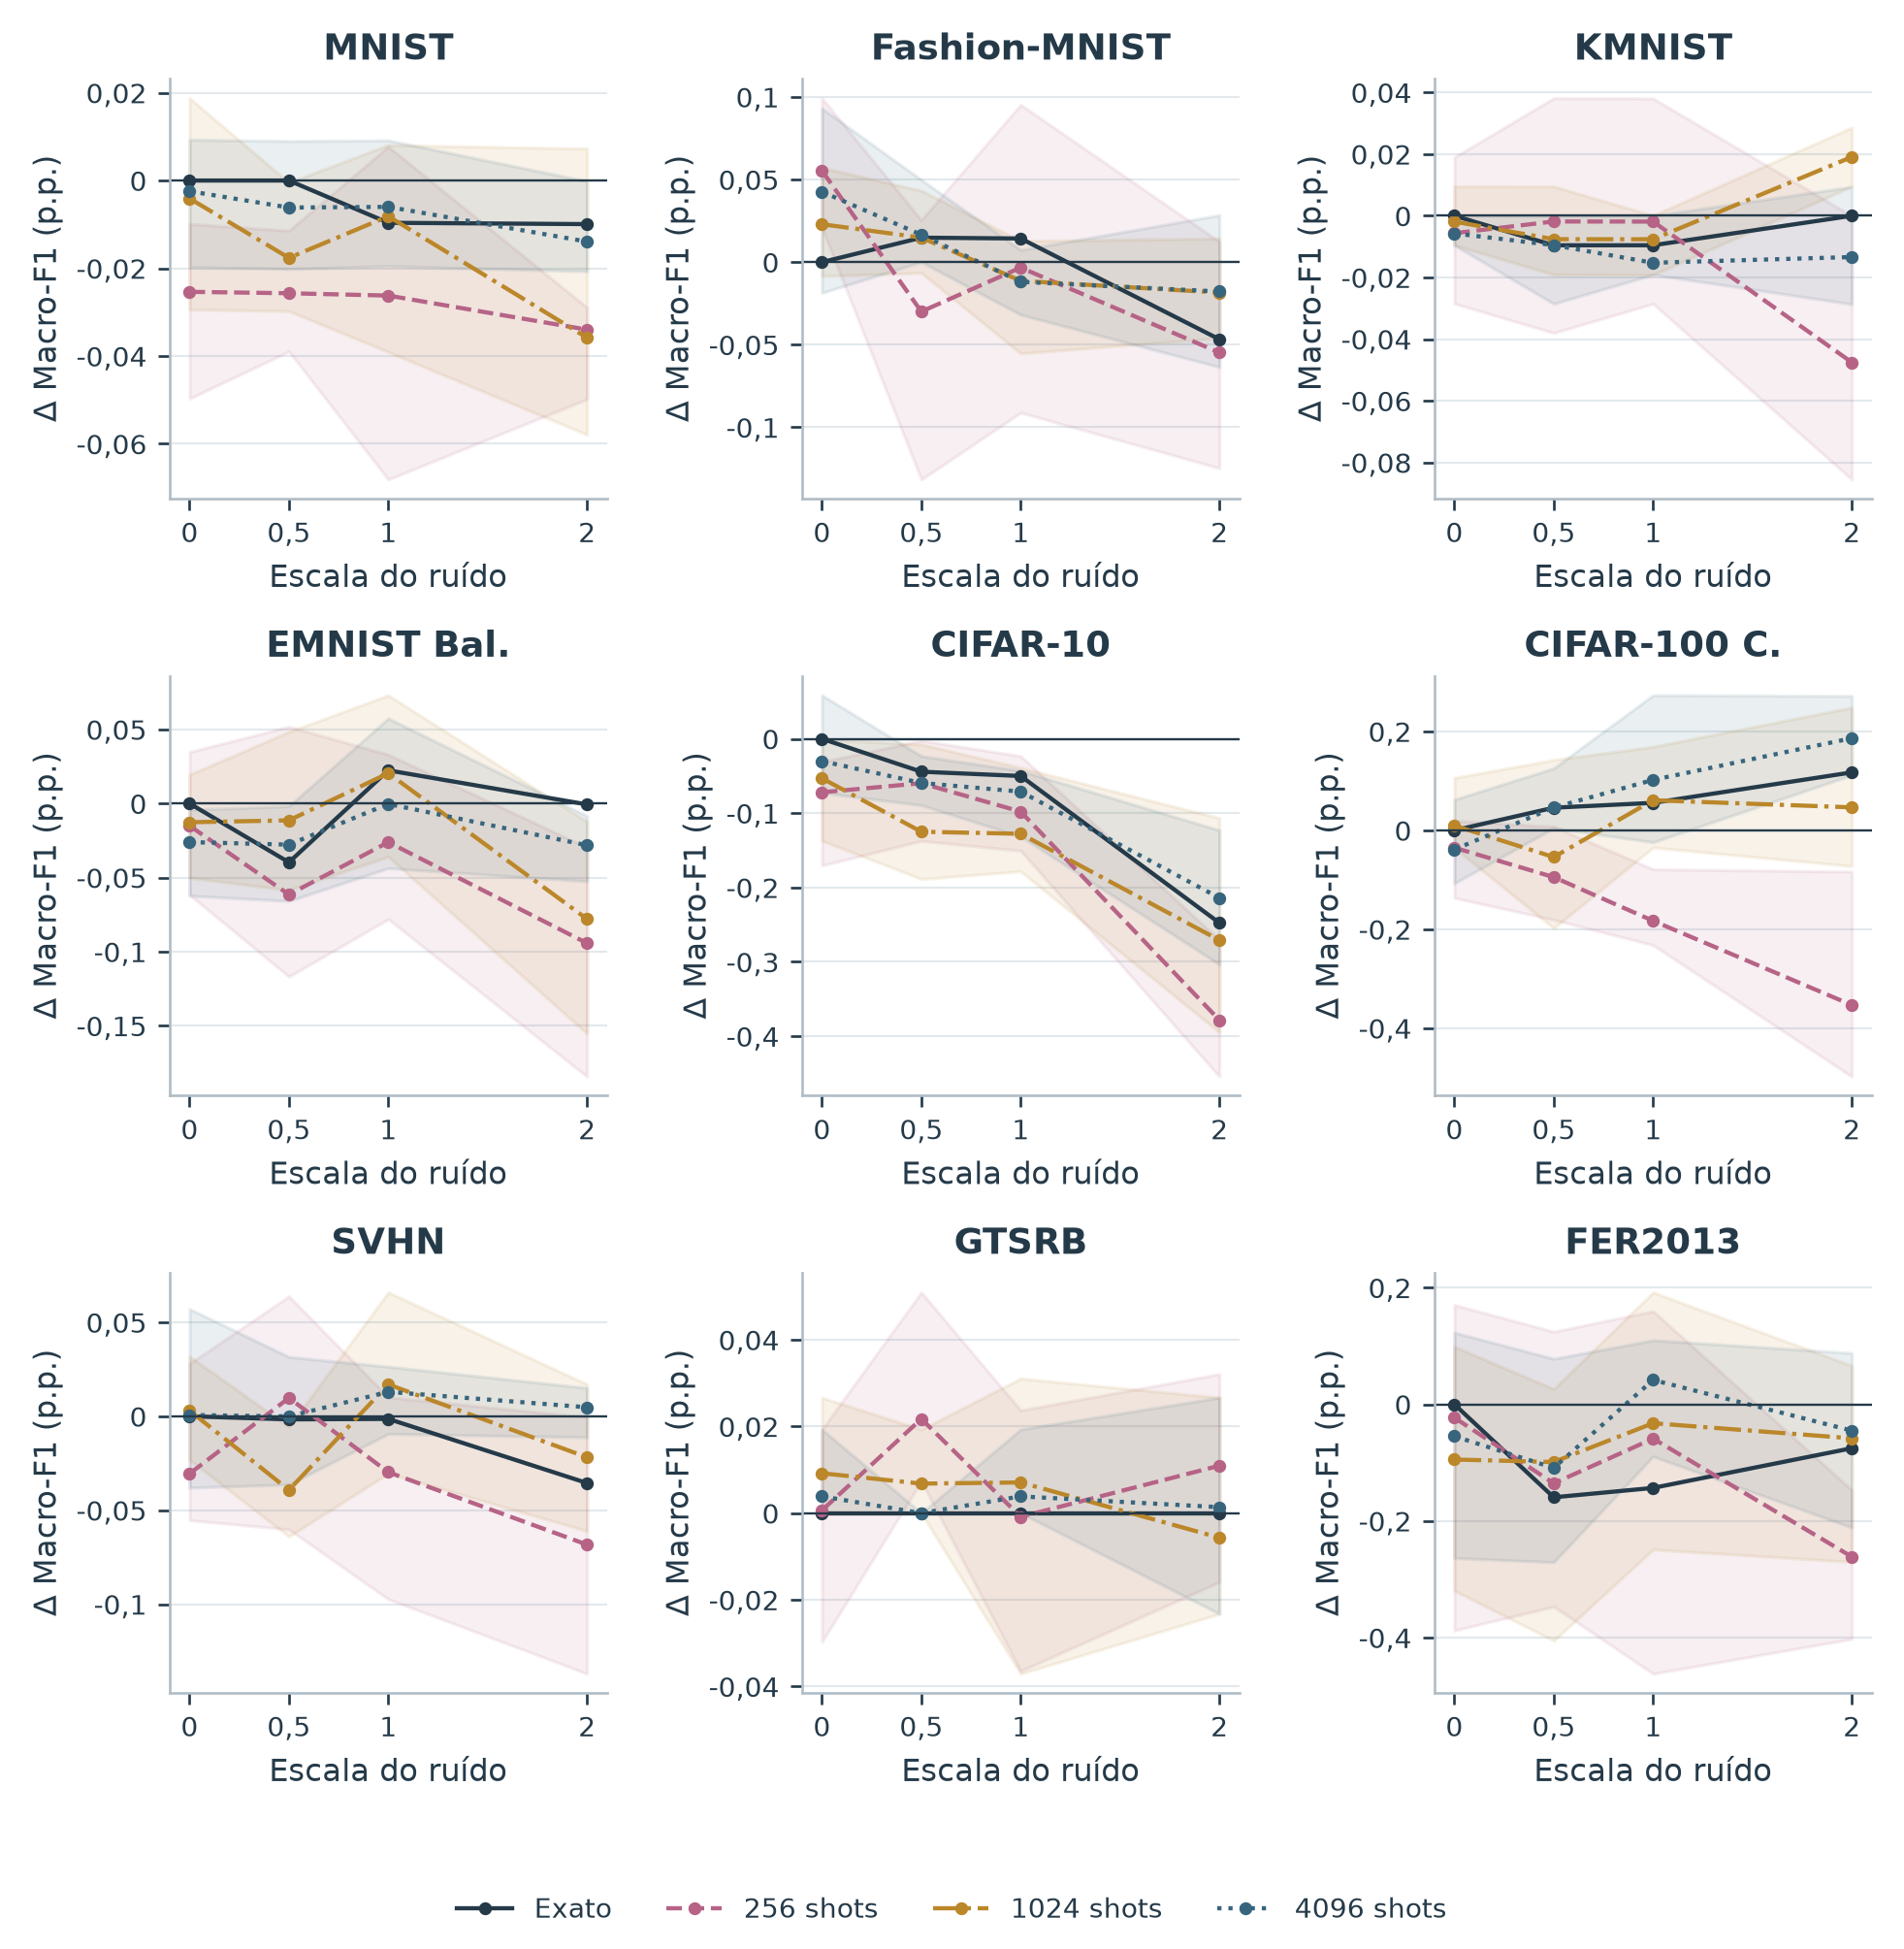
\includegraphics[width=\textwidth,height=0.46\textheight,keepaspectratio]{figura_22_ruido_shots.png}\\[4pt]
      {\footnotesize Ruído e \textit{shots} (Mac/PL): fidelidade cai a 0,51 (ruído 2,0), mas $\Delta$ Macro-F1 típico $< 0{,}10$ p.p.\ (máx.\ $-0{,}38$ p.p.\ CIFAR-10).}
    \end{column}
  \end{columns}
  \fonte{Elaborado pelo autor (2026).}
\end{frame}

% A4
\begin{frame}{Apoio A4: resultados originais de Senokosov et al.\ (2024)}
  \centering
  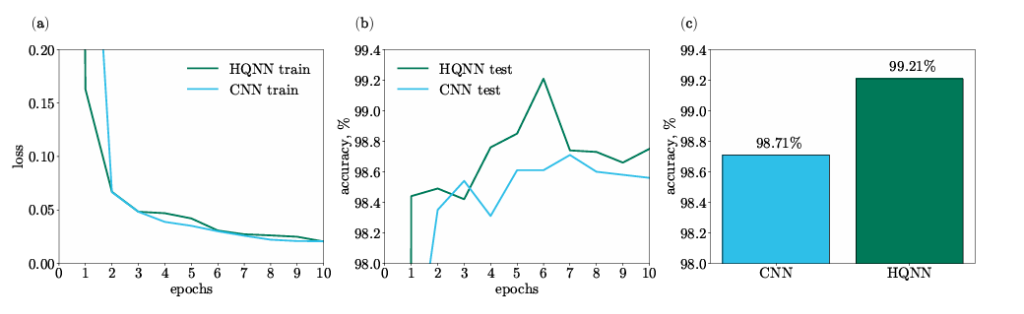
\includegraphics[width=0.95\textwidth,height=0.46\textheight,keepaspectratio]{fig_arxiv2304_mnist_loss_acc.png}
  \vspace{0.15cm}
  \begin{itemize}\footnotesize
    \item MNIST (10 épocas, lote 16, SGD): HQNN-Parallel atingiu 99,21\% (45.194 pesos) vs.\ CNN 98,71\% (372.234 pesos)
    \item No artigo original: Medical MNIST 99,97\% (vs.\ 99,96\%) e CIFAR-10 82,78\% (vs.\ 82,64\%) com $6\times 5$ qubits
  \end{itemize}
  \fonte{Extraído de Senokosov et al.\ (2024) (\texttt{arXiv:2304.09224}, Figura 5).}
\end{frame}

% A5
\begin{frame}{Apoio A5: riscos e limitações metodológicas}
  \footnotesize
  \begin{enumerate}\setlength{\itemsep}{8pt}
    \item Sem emaranhamento cruzado entre os quatro subcircuitos independentes de 5 qubits
    \item Uma semente por configuração (\texttt{seed=42}): sem estimativa de variância inter-sementes
    \item \texttt{Dense20} imagem, vetorial e híbrido diferem em camadas e aumento: sem fator causal único
    \item Dependências auditadas: 67,9\% de \textit{tracks} no GTSRB e 7,02\% de duplicatas + 57 conflitos no FER2013
    \item Restrição integral à simulação clássica local em CPU, sem execução em QPU física
  \end{enumerate}
\end{frame}

% A6
\begin{frame}{Apoio A6: siglas principais}
  \begin{columns}[T,onlytextwidth]
    \begin{column}{0.48\textwidth}
      {\footnotesize
      \begin{tabular}{@{}lR{4.8cm}@{}}
        \toprule
        \textbf{Sigla} & \textbf{Significado} \\
        \midrule
        CNN & Rede Neural Convolucional \\
        PQC & Circuito Quântico Parametrizado \\
        QML & Aprendizado de Máquina Quântico \\
        NISQ & Era Quântica Ruidosa Intermediária \\
        QPU & Unidade de Processamento Quântico \\
        \bottomrule
      \end{tabular}}
    \end{column}
    \begin{column}{0.48\textwidth}
      {\footnotesize
      \begin{tabular}{@{}lR{4.6cm}@{}}
        \toprule
        \textbf{Sigla} & \textbf{Significado} \\
        \midrule
        IR / CV & Razão de Desbal.\ / Coef.\ Variação \\
        ECE / NLL & Erro Calibração / Log-Veross.\ Neg. \\
        RSS & Memória Residente (RAM) \\
        VQA & Algoritmo Quântico Variacional \\
        Grad-CAM & Ativação de Classe por Gradiente \\
        \bottomrule
      \end{tabular}}
    \end{column}
  \end{columns}
\end{frame}

\end{document}
